\documentclass[twoside]{book}

% Packages required by doxygen
\usepackage{calc}
\usepackage{doxygen}
\usepackage{graphicx}
\usepackage[utf8]{inputenc}
\usepackage{makeidx}
\usepackage{multicol}
\usepackage{multirow}
\usepackage{textcomp}
\usepackage[table]{xcolor}

% Font selection
\usepackage[T1]{fontenc}
\usepackage{mathptmx}
\usepackage[scaled=.90]{helvet}
\usepackage{courier}
\usepackage{amssymb}
\usepackage{sectsty}
\renewcommand{\familydefault}{\sfdefault}
\allsectionsfont{%
  \fontseries{bc}\selectfont%
  \color{darkgray}%
}
\renewcommand{\DoxyLabelFont}{%
  \fontseries{bc}\selectfont%
  \color{darkgray}%
}

% Page & text layout
\usepackage{geometry}
\geometry{%
  a4paper,%
  top=2.5cm,%
  bottom=2.5cm,%
  left=2.5cm,%
  right=2.5cm%
}
\tolerance=750
\hfuzz=15pt
\hbadness=750
\setlength{\emergencystretch}{15pt}
\setlength{\parindent}{0cm}
\setlength{\parskip}{0.2cm}
\makeatletter
\renewcommand{\paragraph}{%
  \@startsection{paragraph}{4}{0ex}{-1.0ex}{1.0ex}{%
    \normalfont\normalsize\bfseries\SS@parafont%
  }%
}
\renewcommand{\subparagraph}{%
  \@startsection{subparagraph}{5}{0ex}{-1.0ex}{1.0ex}{%
    \normalfont\normalsize\bfseries\SS@subparafont%
  }%
}
\makeatother

% Headers & footers
\usepackage{fancyhdr}
\pagestyle{fancyplain}
\fancyhead[LE]{\fancyplain{}{\bfseries\thepage}}
\fancyhead[CE]{\fancyplain{}{}}
\fancyhead[RE]{\fancyplain{}{\bfseries\leftmark}}
\fancyhead[LO]{\fancyplain{}{\bfseries\rightmark}}
\fancyhead[CO]{\fancyplain{}{}}
\fancyhead[RO]{\fancyplain{}{\bfseries\thepage}}
\fancyfoot[LE]{\fancyplain{}{}}
\fancyfoot[CE]{\fancyplain{}{}}
\fancyfoot[RE]{\fancyplain{}{\bfseries\scriptsize Generated on Wed Jul 15 2015 21\-:07\-:52 for My Project by Doxygen }}
\fancyfoot[LO]{\fancyplain{}{\bfseries\scriptsize Generated on Wed Jul 15 2015 21\-:07\-:52 for My Project by Doxygen }}
\fancyfoot[CO]{\fancyplain{}{}}
\fancyfoot[RO]{\fancyplain{}{}}
\renewcommand{\footrulewidth}{0.4pt}
\renewcommand{\chaptermark}[1]{%
  \markboth{#1}{}%
}
\renewcommand{\sectionmark}[1]{%
  \markright{\thesection\ #1}%
}

% Indices & bibliography
\usepackage{natbib}
\usepackage[titles]{tocloft}
\setcounter{tocdepth}{3}
\setcounter{secnumdepth}{5}
\makeindex

% Hyperlinks (required, but should be loaded last)
\usepackage{ifpdf}
\ifpdf
  \usepackage[pdftex,pagebackref=true]{hyperref}
\else
  \usepackage[ps2pdf,pagebackref=true]{hyperref}
\fi
\hypersetup{%
  colorlinks=true,%
  linkcolor=blue,%
  citecolor=blue,%
  unicode%
}

% Custom commands
\newcommand{\clearemptydoublepage}{%
  \newpage{\pagestyle{empty}\cleardoublepage}%
}


%===== C O N T E N T S =====

\begin{document}

% Titlepage & ToC
\hypersetup{pageanchor=false}
\pagenumbering{roman}
\begin{titlepage}
\vspace*{7cm}
\begin{center}%
{\Large My Project }\\
\vspace*{1cm}
{\large Generated by Doxygen 1.8.6}\\
\vspace*{0.5cm}
{\small Wed Jul 15 2015 21:07:52}\\
\end{center}
\end{titlepage}
\clearemptydoublepage
\tableofcontents
\clearemptydoublepage
\pagenumbering{arabic}
\hypersetup{pageanchor=true}

%--- Begin generated contents ---
\chapter{Hierarchical Index}
\section{Class Hierarchy}
This inheritance list is sorted roughly, but not completely, alphabetically\-:\begin{DoxyCompactList}
\item \contentsline{section}{my\-\_\-deque$<$ T, A $>$\-:\-:const\-\_\-iterator}{\pageref{classmy__deque_1_1const__iterator}}{}
\item \contentsline{section}{my\-\_\-deque$<$ T, A $>$\-:\-:iterator}{\pageref{classmy__deque_1_1iterator}}{}
\item \contentsline{section}{my\-\_\-deque$<$ T, A $>$}{\pageref{classmy__deque}}{}
\item Test\begin{DoxyCompactList}
\item \contentsline{section}{Deque\-\_\-\-Fixture$<$ T $>$}{\pageref{structDeque__Fixture}}{}
\end{DoxyCompactList}
\end{DoxyCompactList}

\chapter{Class Index}
\section{Class List}
Here are the classes, structs, unions and interfaces with brief descriptions\-:\begin{DoxyCompactList}
\item\contentsline{section}{\hyperlink{classmy__deque_1_1const__iterator}{my\-\_\-deque$<$ T, A $>$\-::const\-\_\-iterator} }{\pageref{classmy__deque_1_1const__iterator}}{}
\item\contentsline{section}{\hyperlink{structDeque__Fixture}{Deque\-\_\-\-Fixture$<$ T $>$} }{\pageref{structDeque__Fixture}}{}
\item\contentsline{section}{\hyperlink{classmy__deque_1_1iterator}{my\-\_\-deque$<$ T, A $>$\-::iterator} }{\pageref{classmy__deque_1_1iterator}}{}
\item\contentsline{section}{\hyperlink{classmy__deque}{my\-\_\-deque$<$ T, A $>$} }{\pageref{classmy__deque}}{}
\end{DoxyCompactList}

\chapter{File Index}
\section{File List}
Here is a list of all files with brief descriptions\-:\begin{DoxyCompactList}
\item\contentsline{section}{\hyperlink{Deque_8h}{Deque.\-h} }{\pageref{Deque_8h}}{}
\item\contentsline{section}{\hyperlink{TestDeque_8c_09_09}{Test\-Deque.\-c++} }{\pageref{TestDeque_8c_09_09}}{}
\end{DoxyCompactList}

\chapter{Class Documentation}
\hypertarget{classmy__deque_1_1const__iterator}{\section{my\-\_\-deque$<$ T, A $>$\-:\-:const\-\_\-iterator Class Reference}
\label{classmy__deque_1_1const__iterator}\index{my\-\_\-deque$<$ T, A $>$\-::const\-\_\-iterator@{my\-\_\-deque$<$ T, A $>$\-::const\-\_\-iterator}}
}


{\ttfamily \#include $<$Deque.\-h$>$}

\subsection*{Public Types}
\begin{DoxyCompactItemize}
\item 
typedef \\*
std\-::bidirectional\-\_\-iterator\-\_\-tag \hyperlink{classmy__deque_1_1const__iterator_a1a84b424e091e49a4af1c13a38621252}{iterator\-\_\-category}
\item 
typedef \hyperlink{classmy__deque_ae9c156c405acc57623a4601ce755596f}{my\-\_\-deque\-::value\-\_\-type} \hyperlink{classmy__deque_1_1const__iterator_adc8d08cb0b0a1dcb50323ba5ab8fdecb}{value\-\_\-type}
\item 
typedef \hyperlink{classmy__deque_ac85676cb2492fbc9bbc6f1a30e9d3c73}{my\-\_\-deque\-::difference\-\_\-type} \hyperlink{classmy__deque_1_1const__iterator_abe3b655aa980c8a12ba486058464c91d}{difference\-\_\-type}
\item 
typedef \hyperlink{classmy__deque_a8fea5edeb2b2cf3dd1246dc3abf9b71b}{my\-\_\-deque\-::const\-\_\-pointer} \hyperlink{classmy__deque_1_1const__iterator_a6a7d42610f3b7e55f38897c151862071}{pointer}
\item 
typedef \hyperlink{classmy__deque_ad50d8b378580088cf77fa43f0640e49c}{my\-\_\-deque\-::const\-\_\-reference} \hyperlink{classmy__deque_1_1const__iterator_a37cd7eef8e73e5a65d7a9d16ba6d3ed2}{reference}
\end{DoxyCompactItemize}
\subsection*{Public Member Functions}
\begin{DoxyCompactItemize}
\item 
\hyperlink{classmy__deque_1_1const__iterator_a119d25762ab3d52a3a81d30870bd9c02}{const\-\_\-iterator} (const \hyperlink{classmy__deque}{my\-\_\-deque} \&q, \hyperlink{classmy__deque_a61e5e5317fe72a381ce4d45f09544b02}{size\-\_\-type} n)
\item 
\hyperlink{classmy__deque_1_1const__iterator_a37cd7eef8e73e5a65d7a9d16ba6d3ed2}{reference} \hyperlink{classmy__deque_1_1const__iterator_a14715989004b54dc6a1bcd3d2ac78a20}{operator$\ast$} () const 
\item 
\hyperlink{classmy__deque_1_1const__iterator_a6a7d42610f3b7e55f38897c151862071}{pointer} \hyperlink{classmy__deque_1_1const__iterator_aef7e08cfcebb0c0932422f420645e1ce}{operator-\/$>$} () const 
\item 
\hyperlink{classmy__deque_1_1const__iterator}{const\-\_\-iterator} \& \hyperlink{classmy__deque_1_1const__iterator_a8bc45a394bb73728fca1ebf90755d662}{operator++} ()
\item 
\hyperlink{classmy__deque_1_1const__iterator}{const\-\_\-iterator} \hyperlink{classmy__deque_1_1const__iterator_adf9ea902391ac993088e7c969c64e4de}{operator++} (int)
\item 
\hyperlink{classmy__deque_1_1const__iterator}{const\-\_\-iterator} \& \hyperlink{classmy__deque_1_1const__iterator_ae5dffda4ac0a8ad59a4954dcdeeb5f98}{operator-\/-\/} ()
\item 
\hyperlink{classmy__deque_1_1const__iterator}{const\-\_\-iterator} \hyperlink{classmy__deque_1_1const__iterator_a83c405a1e0b9672c074aaa933a7127df}{operator-\/-\/} (int)
\item 
\hyperlink{classmy__deque_1_1const__iterator}{const\-\_\-iterator} \& \hyperlink{classmy__deque_1_1const__iterator_a2bbc121cc446855edcb9d20451cae024}{operator+=} (\hyperlink{classmy__deque_1_1const__iterator_abe3b655aa980c8a12ba486058464c91d}{difference\-\_\-type} d)
\item 
\hyperlink{classmy__deque_1_1const__iterator}{const\-\_\-iterator} \& \hyperlink{classmy__deque_1_1const__iterator_ab51576a76fd33fd55be87ca4c467dc96}{operator-\/=} (\hyperlink{classmy__deque_1_1const__iterator_abe3b655aa980c8a12ba486058464c91d}{difference\-\_\-type} d)
\end{DoxyCompactItemize}
\subsection*{Private Member Functions}
\begin{DoxyCompactItemize}
\item 
bool \hyperlink{classmy__deque_1_1const__iterator_ab233485f07a0be8dbc1b41987cc1af42}{valid} () const 
\end{DoxyCompactItemize}
\subsection*{Private Attributes}
\begin{DoxyCompactItemize}
\item 
const \hyperlink{classmy__deque}{my\-\_\-deque} $\ast$ \hyperlink{classmy__deque_1_1const__iterator_a9bb01f756f5c5e283d8d83d3fcae876a}{\-\_\-q}
\item 
\hyperlink{classmy__deque_a61e5e5317fe72a381ce4d45f09544b02}{size\-\_\-type} \hyperlink{classmy__deque_1_1const__iterator_a96e9c925cd20cfbbd18b9f5891bee5ff}{\-\_\-i}
\end{DoxyCompactItemize}
\subsection*{Friends}
\begin{DoxyCompactItemize}
\item 
bool \hyperlink{classmy__deque_1_1const__iterator_a772a728ee48f5cb8904aaae842b0eb82}{operator==} (const \hyperlink{classmy__deque_1_1const__iterator}{const\-\_\-iterator} \&lhs, const \hyperlink{classmy__deque_1_1const__iterator}{const\-\_\-iterator} \&rhs)
\item 
bool \hyperlink{classmy__deque_1_1const__iterator_a12d66edf831aeec4957931d7f7945d90}{operator!=} (const \hyperlink{classmy__deque_1_1const__iterator}{const\-\_\-iterator} \&lhs, const \hyperlink{classmy__deque_1_1const__iterator}{const\-\_\-iterator} \&rhs)
\item 
\hyperlink{classmy__deque_1_1const__iterator}{const\-\_\-iterator} \hyperlink{classmy__deque_1_1const__iterator_ab6ce7b11eff6ef34762c30e4e96a86a0}{operator+} (\hyperlink{classmy__deque_1_1const__iterator}{const\-\_\-iterator} lhs, \hyperlink{classmy__deque_1_1const__iterator_abe3b655aa980c8a12ba486058464c91d}{difference\-\_\-type} rhs)
\item 
\hyperlink{classmy__deque_1_1const__iterator}{const\-\_\-iterator} \hyperlink{classmy__deque_1_1const__iterator_a41934331896eac6321161ff28c21fb29}{operator-\/} (\hyperlink{classmy__deque_1_1const__iterator}{const\-\_\-iterator} lhs, \hyperlink{classmy__deque_1_1const__iterator_abe3b655aa980c8a12ba486058464c91d}{difference\-\_\-type} rhs)
\end{DoxyCompactItemize}


\subsection{Member Typedef Documentation}
\hypertarget{classmy__deque_1_1const__iterator_abe3b655aa980c8a12ba486058464c91d}{\index{my\-\_\-deque\-::const\-\_\-iterator@{my\-\_\-deque\-::const\-\_\-iterator}!difference\-\_\-type@{difference\-\_\-type}}
\index{difference\-\_\-type@{difference\-\_\-type}!my_deque::const_iterator@{my\-\_\-deque\-::const\-\_\-iterator}}
\subsubsection[{difference\-\_\-type}]{\setlength{\rightskip}{0pt plus 5cm}template$<$typename T , typename A  = std\-::allocator$<$\-T$>$$>$ typedef {\bf my\-\_\-deque\-::difference\-\_\-type} {\bf my\-\_\-deque}$<$ T, A $>$\-::{\bf const\-\_\-iterator\-::difference\-\_\-type}}}\label{classmy__deque_1_1const__iterator_abe3b655aa980c8a12ba486058464c91d}
\hypertarget{classmy__deque_1_1const__iterator_a1a84b424e091e49a4af1c13a38621252}{\index{my\-\_\-deque\-::const\-\_\-iterator@{my\-\_\-deque\-::const\-\_\-iterator}!iterator\-\_\-category@{iterator\-\_\-category}}
\index{iterator\-\_\-category@{iterator\-\_\-category}!my_deque::const_iterator@{my\-\_\-deque\-::const\-\_\-iterator}}
\subsubsection[{iterator\-\_\-category}]{\setlength{\rightskip}{0pt plus 5cm}template$<$typename T , typename A  = std\-::allocator$<$\-T$>$$>$ typedef std\-::bidirectional\-\_\-iterator\-\_\-tag {\bf my\-\_\-deque}$<$ T, A $>$\-::{\bf const\-\_\-iterator\-::iterator\-\_\-category}}}\label{classmy__deque_1_1const__iterator_a1a84b424e091e49a4af1c13a38621252}
\hypertarget{classmy__deque_1_1const__iterator_a6a7d42610f3b7e55f38897c151862071}{\index{my\-\_\-deque\-::const\-\_\-iterator@{my\-\_\-deque\-::const\-\_\-iterator}!pointer@{pointer}}
\index{pointer@{pointer}!my_deque::const_iterator@{my\-\_\-deque\-::const\-\_\-iterator}}
\subsubsection[{pointer}]{\setlength{\rightskip}{0pt plus 5cm}template$<$typename T , typename A  = std\-::allocator$<$\-T$>$$>$ typedef {\bf my\-\_\-deque\-::const\-\_\-pointer} {\bf my\-\_\-deque}$<$ T, A $>$\-::{\bf const\-\_\-iterator\-::pointer}}}\label{classmy__deque_1_1const__iterator_a6a7d42610f3b7e55f38897c151862071}
\hypertarget{classmy__deque_1_1const__iterator_a37cd7eef8e73e5a65d7a9d16ba6d3ed2}{\index{my\-\_\-deque\-::const\-\_\-iterator@{my\-\_\-deque\-::const\-\_\-iterator}!reference@{reference}}
\index{reference@{reference}!my_deque::const_iterator@{my\-\_\-deque\-::const\-\_\-iterator}}
\subsubsection[{reference}]{\setlength{\rightskip}{0pt plus 5cm}template$<$typename T , typename A  = std\-::allocator$<$\-T$>$$>$ typedef {\bf my\-\_\-deque\-::const\-\_\-reference} {\bf my\-\_\-deque}$<$ T, A $>$\-::{\bf const\-\_\-iterator\-::reference}}}\label{classmy__deque_1_1const__iterator_a37cd7eef8e73e5a65d7a9d16ba6d3ed2}
\hypertarget{classmy__deque_1_1const__iterator_adc8d08cb0b0a1dcb50323ba5ab8fdecb}{\index{my\-\_\-deque\-::const\-\_\-iterator@{my\-\_\-deque\-::const\-\_\-iterator}!value\-\_\-type@{value\-\_\-type}}
\index{value\-\_\-type@{value\-\_\-type}!my_deque::const_iterator@{my\-\_\-deque\-::const\-\_\-iterator}}
\subsubsection[{value\-\_\-type}]{\setlength{\rightskip}{0pt plus 5cm}template$<$typename T , typename A  = std\-::allocator$<$\-T$>$$>$ typedef {\bf my\-\_\-deque\-::value\-\_\-type} {\bf my\-\_\-deque}$<$ T, A $>$\-::{\bf const\-\_\-iterator\-::value\-\_\-type}}}\label{classmy__deque_1_1const__iterator_adc8d08cb0b0a1dcb50323ba5ab8fdecb}


\subsection{Constructor \& Destructor Documentation}
\hypertarget{classmy__deque_1_1const__iterator_a119d25762ab3d52a3a81d30870bd9c02}{\index{my\-\_\-deque\-::const\-\_\-iterator@{my\-\_\-deque\-::const\-\_\-iterator}!const\-\_\-iterator@{const\-\_\-iterator}}
\index{const\-\_\-iterator@{const\-\_\-iterator}!my_deque::const_iterator@{my\-\_\-deque\-::const\-\_\-iterator}}
\subsubsection[{const\-\_\-iterator}]{\setlength{\rightskip}{0pt plus 5cm}template$<$typename T , typename A  = std\-::allocator$<$\-T$>$$>$ {\bf my\-\_\-deque}$<$ T, A $>$\-::const\-\_\-iterator\-::const\-\_\-iterator (
\begin{DoxyParamCaption}
\item[{const {\bf my\-\_\-deque} \&}]{q, }
\item[{{\bf size\-\_\-type}}]{n}
\end{DoxyParamCaption}
)\hspace{0.3cm}{\ttfamily [inline]}}}\label{classmy__deque_1_1const__iterator_a119d25762ab3d52a3a81d30870bd9c02}
Construct a const\-\_\-terator for a const \hyperlink{classmy__deque}{my\-\_\-deque} 
\begin{DoxyParams}{Parameters}
{\em q} & a const \hyperlink{classmy__deque}{my\-\_\-deque} to iterate over \\
\hline
{\em n} & an index into the \hyperlink{classmy__deque}{my\-\_\-deque} \\
\hline
\end{DoxyParams}


\subsection{Member Function Documentation}
\hypertarget{classmy__deque_1_1const__iterator_a14715989004b54dc6a1bcd3d2ac78a20}{\index{my\-\_\-deque\-::const\-\_\-iterator@{my\-\_\-deque\-::const\-\_\-iterator}!operator$\ast$@{operator$\ast$}}
\index{operator$\ast$@{operator$\ast$}!my_deque::const_iterator@{my\-\_\-deque\-::const\-\_\-iterator}}
\subsubsection[{operator$\ast$}]{\setlength{\rightskip}{0pt plus 5cm}template$<$typename T , typename A  = std\-::allocator$<$\-T$>$$>$ {\bf reference} {\bf my\-\_\-deque}$<$ T, A $>$\-::const\-\_\-iterator\-::operator$\ast$ (
\begin{DoxyParamCaption}
{}
\end{DoxyParamCaption}
) const\hspace{0.3cm}{\ttfamily [inline]}}}\label{classmy__deque_1_1const__iterator_a14715989004b54dc6a1bcd3d2ac78a20}
Dereference this \hyperlink{classmy__deque_1_1const__iterator}{const\-\_\-iterator} to get the underlying element \begin{DoxyReturn}{Returns}
a reference to an element of this \hyperlink{classmy__deque}{my\-\_\-deque} 
\end{DoxyReturn}
\hypertarget{classmy__deque_1_1const__iterator_a8bc45a394bb73728fca1ebf90755d662}{\index{my\-\_\-deque\-::const\-\_\-iterator@{my\-\_\-deque\-::const\-\_\-iterator}!operator++@{operator++}}
\index{operator++@{operator++}!my_deque::const_iterator@{my\-\_\-deque\-::const\-\_\-iterator}}
\subsubsection[{operator++}]{\setlength{\rightskip}{0pt plus 5cm}template$<$typename T , typename A  = std\-::allocator$<$\-T$>$$>$ {\bf const\-\_\-iterator}\& {\bf my\-\_\-deque}$<$ T, A $>$\-::const\-\_\-iterator\-::operator++ (
\begin{DoxyParamCaption}
{}
\end{DoxyParamCaption}
)\hspace{0.3cm}{\ttfamily [inline]}}}\label{classmy__deque_1_1const__iterator_a8bc45a394bb73728fca1ebf90755d662}
Pre increment this \hyperlink{classmy__deque_1_1const__iterator}{const\-\_\-iterator} \begin{DoxyReturn}{Returns}
this \hyperlink{classmy__deque_1_1const__iterator}{const\-\_\-iterator} 
\end{DoxyReturn}
\hypertarget{classmy__deque_1_1const__iterator_adf9ea902391ac993088e7c969c64e4de}{\index{my\-\_\-deque\-::const\-\_\-iterator@{my\-\_\-deque\-::const\-\_\-iterator}!operator++@{operator++}}
\index{operator++@{operator++}!my_deque::const_iterator@{my\-\_\-deque\-::const\-\_\-iterator}}
\subsubsection[{operator++}]{\setlength{\rightskip}{0pt plus 5cm}template$<$typename T , typename A  = std\-::allocator$<$\-T$>$$>$ {\bf const\-\_\-iterator} {\bf my\-\_\-deque}$<$ T, A $>$\-::const\-\_\-iterator\-::operator++ (
\begin{DoxyParamCaption}
\item[{int}]{}
\end{DoxyParamCaption}
)\hspace{0.3cm}{\ttfamily [inline]}}}\label{classmy__deque_1_1const__iterator_adf9ea902391ac993088e7c969c64e4de}
Post increment this \hyperlink{classmy__deque_1_1const__iterator}{const\-\_\-iterator} \begin{DoxyReturn}{Returns}
this \hyperlink{classmy__deque_1_1const__iterator}{const\-\_\-iterator} 
\end{DoxyReturn}
\hypertarget{classmy__deque_1_1const__iterator_a2bbc121cc446855edcb9d20451cae024}{\index{my\-\_\-deque\-::const\-\_\-iterator@{my\-\_\-deque\-::const\-\_\-iterator}!operator+=@{operator+=}}
\index{operator+=@{operator+=}!my_deque::const_iterator@{my\-\_\-deque\-::const\-\_\-iterator}}
\subsubsection[{operator+=}]{\setlength{\rightskip}{0pt plus 5cm}template$<$typename T , typename A  = std\-::allocator$<$\-T$>$$>$ {\bf const\-\_\-iterator}\& {\bf my\-\_\-deque}$<$ T, A $>$\-::const\-\_\-iterator\-::operator+= (
\begin{DoxyParamCaption}
\item[{{\bf difference\-\_\-type}}]{d}
\end{DoxyParamCaption}
)\hspace{0.3cm}{\ttfamily [inline]}}}\label{classmy__deque_1_1const__iterator_a2bbc121cc446855edcb9d20451cae024}
Add a numerical value to this \hyperlink{classmy__deque_1_1const__iterator}{const\-\_\-iterator} 
\begin{DoxyParams}{Parameters}
{\em d} & a numerical value \\
\hline
\end{DoxyParams}
\begin{DoxyReturn}{Returns}
this \hyperlink{classmy__deque_1_1const__iterator}{const\-\_\-iterator} 
\end{DoxyReturn}
\hypertarget{classmy__deque_1_1const__iterator_ae5dffda4ac0a8ad59a4954dcdeeb5f98}{\index{my\-\_\-deque\-::const\-\_\-iterator@{my\-\_\-deque\-::const\-\_\-iterator}!operator-\/-\/@{operator-\/-\/}}
\index{operator-\/-\/@{operator-\/-\/}!my_deque::const_iterator@{my\-\_\-deque\-::const\-\_\-iterator}}
\subsubsection[{operator-\/-\/}]{\setlength{\rightskip}{0pt plus 5cm}template$<$typename T , typename A  = std\-::allocator$<$\-T$>$$>$ {\bf const\-\_\-iterator}\& {\bf my\-\_\-deque}$<$ T, A $>$\-::const\-\_\-iterator\-::operator-\/-\/ (
\begin{DoxyParamCaption}
{}
\end{DoxyParamCaption}
)\hspace{0.3cm}{\ttfamily [inline]}}}\label{classmy__deque_1_1const__iterator_ae5dffda4ac0a8ad59a4954dcdeeb5f98}
Pre decrement this \hyperlink{classmy__deque_1_1const__iterator}{const\-\_\-iterator} \begin{DoxyReturn}{Returns}
this \hyperlink{classmy__deque_1_1const__iterator}{const\-\_\-iterator} 
\end{DoxyReturn}
\hypertarget{classmy__deque_1_1const__iterator_a83c405a1e0b9672c074aaa933a7127df}{\index{my\-\_\-deque\-::const\-\_\-iterator@{my\-\_\-deque\-::const\-\_\-iterator}!operator-\/-\/@{operator-\/-\/}}
\index{operator-\/-\/@{operator-\/-\/}!my_deque::const_iterator@{my\-\_\-deque\-::const\-\_\-iterator}}
\subsubsection[{operator-\/-\/}]{\setlength{\rightskip}{0pt plus 5cm}template$<$typename T , typename A  = std\-::allocator$<$\-T$>$$>$ {\bf const\-\_\-iterator} {\bf my\-\_\-deque}$<$ T, A $>$\-::const\-\_\-iterator\-::operator-\/-\/ (
\begin{DoxyParamCaption}
\item[{int}]{}
\end{DoxyParamCaption}
)\hspace{0.3cm}{\ttfamily [inline]}}}\label{classmy__deque_1_1const__iterator_a83c405a1e0b9672c074aaa933a7127df}
Post decrement this \hyperlink{classmy__deque_1_1const__iterator}{const\-\_\-iterator} \begin{DoxyReturn}{Returns}
this \hyperlink{classmy__deque_1_1const__iterator}{const\-\_\-iterator} 
\end{DoxyReturn}
\hypertarget{classmy__deque_1_1const__iterator_ab51576a76fd33fd55be87ca4c467dc96}{\index{my\-\_\-deque\-::const\-\_\-iterator@{my\-\_\-deque\-::const\-\_\-iterator}!operator-\/=@{operator-\/=}}
\index{operator-\/=@{operator-\/=}!my_deque::const_iterator@{my\-\_\-deque\-::const\-\_\-iterator}}
\subsubsection[{operator-\/=}]{\setlength{\rightskip}{0pt plus 5cm}template$<$typename T , typename A  = std\-::allocator$<$\-T$>$$>$ {\bf const\-\_\-iterator}\& {\bf my\-\_\-deque}$<$ T, A $>$\-::const\-\_\-iterator\-::operator-\/= (
\begin{DoxyParamCaption}
\item[{{\bf difference\-\_\-type}}]{d}
\end{DoxyParamCaption}
)\hspace{0.3cm}{\ttfamily [inline]}}}\label{classmy__deque_1_1const__iterator_ab51576a76fd33fd55be87ca4c467dc96}
Subtract a numerical value from this \hyperlink{classmy__deque_1_1const__iterator}{const\-\_\-iterator} 
\begin{DoxyParams}{Parameters}
{\em d} & a numerical value \\
\hline
\end{DoxyParams}
\begin{DoxyReturn}{Returns}
this \hyperlink{classmy__deque_1_1const__iterator}{const\-\_\-iterator} 
\end{DoxyReturn}
\hypertarget{classmy__deque_1_1const__iterator_aef7e08cfcebb0c0932422f420645e1ce}{\index{my\-\_\-deque\-::const\-\_\-iterator@{my\-\_\-deque\-::const\-\_\-iterator}!operator-\/$>$@{operator-\/$>$}}
\index{operator-\/$>$@{operator-\/$>$}!my_deque::const_iterator@{my\-\_\-deque\-::const\-\_\-iterator}}
\subsubsection[{operator-\/$>$}]{\setlength{\rightskip}{0pt plus 5cm}template$<$typename T , typename A  = std\-::allocator$<$\-T$>$$>$ {\bf pointer} {\bf my\-\_\-deque}$<$ T, A $>$\-::const\-\_\-iterator\-::operator-\/$>$ (
\begin{DoxyParamCaption}
{}
\end{DoxyParamCaption}
) const\hspace{0.3cm}{\ttfamily [inline]}}}\label{classmy__deque_1_1const__iterator_aef7e08cfcebb0c0932422f420645e1ce}
Get the pointer to the underlying element of this \hyperlink{classmy__deque_1_1const__iterator}{const\-\_\-iterator} \begin{DoxyReturn}{Returns}
a pointer to an element of this \hyperlink{classmy__deque}{my\-\_\-deque} 
\end{DoxyReturn}
\hypertarget{classmy__deque_1_1const__iterator_ab233485f07a0be8dbc1b41987cc1af42}{\index{my\-\_\-deque\-::const\-\_\-iterator@{my\-\_\-deque\-::const\-\_\-iterator}!valid@{valid}}
\index{valid@{valid}!my_deque::const_iterator@{my\-\_\-deque\-::const\-\_\-iterator}}
\subsubsection[{valid}]{\setlength{\rightskip}{0pt plus 5cm}template$<$typename T , typename A  = std\-::allocator$<$\-T$>$$>$ bool {\bf my\-\_\-deque}$<$ T, A $>$\-::const\-\_\-iterator\-::valid (
\begin{DoxyParamCaption}
{}
\end{DoxyParamCaption}
) const\hspace{0.3cm}{\ttfamily [inline]}, {\ttfamily [private]}}}\label{classmy__deque_1_1const__iterator_ab233485f07a0be8dbc1b41987cc1af42}
Check to make sure an iterator is valid \begin{DoxyReturn}{Returns}
true if the iterator index \-\_\-i is less than or equal to the \hyperlink{classmy__deque}{my\-\_\-deque} size 
\end{DoxyReturn}


\subsection{Friends And Related Function Documentation}
\hypertarget{classmy__deque_1_1const__iterator_a12d66edf831aeec4957931d7f7945d90}{\index{my\-\_\-deque\-::const\-\_\-iterator@{my\-\_\-deque\-::const\-\_\-iterator}!operator!=@{operator!=}}
\index{operator!=@{operator!=}!my_deque::const_iterator@{my\-\_\-deque\-::const\-\_\-iterator}}
\subsubsection[{operator!=}]{\setlength{\rightskip}{0pt plus 5cm}template$<$typename T , typename A  = std\-::allocator$<$\-T$>$$>$ bool operator!= (
\begin{DoxyParamCaption}
\item[{const {\bf const\-\_\-iterator} \&}]{lhs, }
\item[{const {\bf const\-\_\-iterator} \&}]{rhs}
\end{DoxyParamCaption}
)\hspace{0.3cm}{\ttfamily [friend]}}}\label{classmy__deque_1_1const__iterator_a12d66edf831aeec4957931d7f7945d90}
Check to see if two const\-\_\-iterators are not equivalent 
\begin{DoxyParams}{Parameters}
{\em lhs} & a const \hyperlink{classmy__deque_1_1const__iterator}{const\-\_\-iterator} reference \\
\hline
{\em rhs} & a const \hyperlink{classmy__deque_1_1const__iterator}{const\-\_\-iterator} reference \\
\hline
\end{DoxyParams}
\begin{DoxyReturn}{Returns}
true if lhs is not equivalent to rhs 
\end{DoxyReturn}
\hypertarget{classmy__deque_1_1const__iterator_ab6ce7b11eff6ef34762c30e4e96a86a0}{\index{my\-\_\-deque\-::const\-\_\-iterator@{my\-\_\-deque\-::const\-\_\-iterator}!operator+@{operator+}}
\index{operator+@{operator+}!my_deque::const_iterator@{my\-\_\-deque\-::const\-\_\-iterator}}
\subsubsection[{operator+}]{\setlength{\rightskip}{0pt plus 5cm}template$<$typename T , typename A  = std\-::allocator$<$\-T$>$$>$ {\bf const\-\_\-iterator} operator+ (
\begin{DoxyParamCaption}
\item[{{\bf const\-\_\-iterator}}]{lhs, }
\item[{{\bf difference\-\_\-type}}]{rhs}
\end{DoxyParamCaption}
)\hspace{0.3cm}{\ttfamily [friend]}}}\label{classmy__deque_1_1const__iterator_ab6ce7b11eff6ef34762c30e4e96a86a0}
Add a value to a \hyperlink{classmy__deque_1_1const__iterator}{const\-\_\-iterator} 
\begin{DoxyParams}{Parameters}
{\em lhs} & a \hyperlink{classmy__deque_1_1const__iterator}{const\-\_\-iterator} \\
\hline
{\em rhs} & a number to add to lhs \\
\hline
\end{DoxyParams}
\begin{DoxyReturn}{Returns}
a new \hyperlink{classmy__deque_1_1const__iterator}{const\-\_\-iterator} 
\end{DoxyReturn}
\hypertarget{classmy__deque_1_1const__iterator_a41934331896eac6321161ff28c21fb29}{\index{my\-\_\-deque\-::const\-\_\-iterator@{my\-\_\-deque\-::const\-\_\-iterator}!operator-\/@{operator-\/}}
\index{operator-\/@{operator-\/}!my_deque::const_iterator@{my\-\_\-deque\-::const\-\_\-iterator}}
\subsubsection[{operator-\/}]{\setlength{\rightskip}{0pt plus 5cm}template$<$typename T , typename A  = std\-::allocator$<$\-T$>$$>$ {\bf const\-\_\-iterator} operator-\/ (
\begin{DoxyParamCaption}
\item[{{\bf const\-\_\-iterator}}]{lhs, }
\item[{{\bf difference\-\_\-type}}]{rhs}
\end{DoxyParamCaption}
)\hspace{0.3cm}{\ttfamily [friend]}}}\label{classmy__deque_1_1const__iterator_a41934331896eac6321161ff28c21fb29}
Subtract a value from a \hyperlink{classmy__deque_1_1const__iterator}{const\-\_\-iterator} 
\begin{DoxyParams}{Parameters}
{\em lhs} & an \hyperlink{classmy__deque_1_1const__iterator}{const\-\_\-iterator} \\
\hline
{\em rhs} & a number to subtract from lhs \\
\hline
\end{DoxyParams}
\begin{DoxyReturn}{Returns}
a new \hyperlink{classmy__deque_1_1const__iterator}{const\-\_\-iterator} 
\end{DoxyReturn}
\hypertarget{classmy__deque_1_1const__iterator_a772a728ee48f5cb8904aaae842b0eb82}{\index{my\-\_\-deque\-::const\-\_\-iterator@{my\-\_\-deque\-::const\-\_\-iterator}!operator==@{operator==}}
\index{operator==@{operator==}!my_deque::const_iterator@{my\-\_\-deque\-::const\-\_\-iterator}}
\subsubsection[{operator==}]{\setlength{\rightskip}{0pt plus 5cm}template$<$typename T , typename A  = std\-::allocator$<$\-T$>$$>$ bool operator== (
\begin{DoxyParamCaption}
\item[{const {\bf const\-\_\-iterator} \&}]{lhs, }
\item[{const {\bf const\-\_\-iterator} \&}]{rhs}
\end{DoxyParamCaption}
)\hspace{0.3cm}{\ttfamily [friend]}}}\label{classmy__deque_1_1const__iterator_a772a728ee48f5cb8904aaae842b0eb82}
Check to see if two iterators are equivalent 
\begin{DoxyParams}{Parameters}
{\em lhs} & a const iterator reference \\
\hline
{\em rhs} & a const iterator reference \\
\hline
\end{DoxyParams}
\begin{DoxyReturn}{Returns}
true if lhs is equivalent to rhs 
\end{DoxyReturn}


\subsection{Member Data Documentation}
\hypertarget{classmy__deque_1_1const__iterator_a96e9c925cd20cfbbd18b9f5891bee5ff}{\index{my\-\_\-deque\-::const\-\_\-iterator@{my\-\_\-deque\-::const\-\_\-iterator}!\-\_\-i@{\-\_\-i}}
\index{\-\_\-i@{\-\_\-i}!my_deque::const_iterator@{my\-\_\-deque\-::const\-\_\-iterator}}
\subsubsection[{\-\_\-i}]{\setlength{\rightskip}{0pt plus 5cm}template$<$typename T , typename A  = std\-::allocator$<$\-T$>$$>$ {\bf size\-\_\-type} {\bf my\-\_\-deque}$<$ T, A $>$\-::const\-\_\-iterator\-::\-\_\-i\hspace{0.3cm}{\ttfamily [private]}}}\label{classmy__deque_1_1const__iterator_a96e9c925cd20cfbbd18b9f5891bee5ff}
\hypertarget{classmy__deque_1_1const__iterator_a9bb01f756f5c5e283d8d83d3fcae876a}{\index{my\-\_\-deque\-::const\-\_\-iterator@{my\-\_\-deque\-::const\-\_\-iterator}!\-\_\-q@{\-\_\-q}}
\index{\-\_\-q@{\-\_\-q}!my_deque::const_iterator@{my\-\_\-deque\-::const\-\_\-iterator}}
\subsubsection[{\-\_\-q}]{\setlength{\rightskip}{0pt plus 5cm}template$<$typename T , typename A  = std\-::allocator$<$\-T$>$$>$ const {\bf my\-\_\-deque}$\ast$ {\bf my\-\_\-deque}$<$ T, A $>$\-::const\-\_\-iterator\-::\-\_\-q\hspace{0.3cm}{\ttfamily [private]}}}\label{classmy__deque_1_1const__iterator_a9bb01f756f5c5e283d8d83d3fcae876a}


The documentation for this class was generated from the following file\-:\begin{DoxyCompactItemize}
\item 
\hyperlink{Deque_8h}{Deque.\-h}\end{DoxyCompactItemize}

\hypertarget{structDeque__Fixture}{\section{Deque\-\_\-\-Fixture$<$ T $>$ Struct Template Reference}
\label{structDeque__Fixture}\index{Deque\-\_\-\-Fixture$<$ T $>$@{Deque\-\_\-\-Fixture$<$ T $>$}}
}
Inheritance diagram for Deque\-\_\-\-Fixture$<$ T $>$\-:\begin{figure}[H]
\begin{center}
\leavevmode
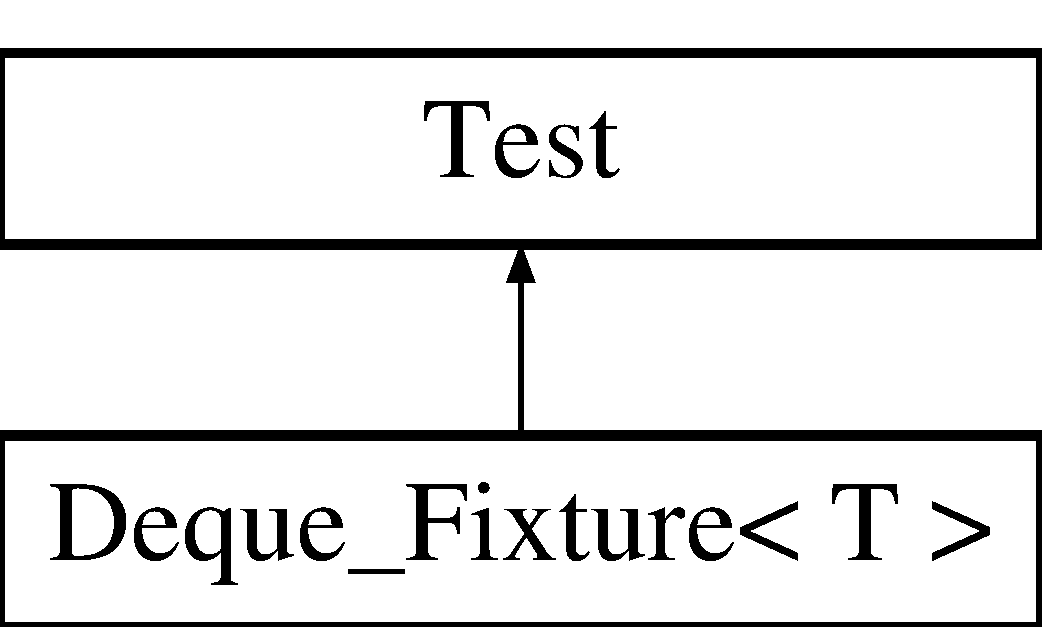
\includegraphics[height=2.000000cm]{structDeque__Fixture}
\end{center}
\end{figure}
\subsection*{Public Types}
\begin{DoxyCompactItemize}
\item 
typedef T \hyperlink{structDeque__Fixture_abca7ea1144ae2545c5d1d516696d6cd1}{deque\-\_\-t}
\item 
typedef deque\-\_\-t\-::value\-\_\-type \hyperlink{structDeque__Fixture_a6f961ca3cd056defc89d8e523807c88e}{value\-\_\-t}
\end{DoxyCompactItemize}


\subsection{Member Typedef Documentation}
\hypertarget{structDeque__Fixture_abca7ea1144ae2545c5d1d516696d6cd1}{\index{Deque\-\_\-\-Fixture@{Deque\-\_\-\-Fixture}!deque\-\_\-t@{deque\-\_\-t}}
\index{deque\-\_\-t@{deque\-\_\-t}!Deque_Fixture@{Deque\-\_\-\-Fixture}}
\subsubsection[{deque\-\_\-t}]{\setlength{\rightskip}{0pt plus 5cm}template$<$typename T $>$ typedef T {\bf Deque\-\_\-\-Fixture}$<$ T $>$\-::{\bf deque\-\_\-t}}}\label{structDeque__Fixture_abca7ea1144ae2545c5d1d516696d6cd1}
\hypertarget{structDeque__Fixture_a6f961ca3cd056defc89d8e523807c88e}{\index{Deque\-\_\-\-Fixture@{Deque\-\_\-\-Fixture}!value\-\_\-t@{value\-\_\-t}}
\index{value\-\_\-t@{value\-\_\-t}!Deque_Fixture@{Deque\-\_\-\-Fixture}}
\subsubsection[{value\-\_\-t}]{\setlength{\rightskip}{0pt plus 5cm}template$<$typename T $>$ typedef deque\-\_\-t\-::value\-\_\-type {\bf Deque\-\_\-\-Fixture}$<$ T $>$\-::{\bf value\-\_\-t}}}\label{structDeque__Fixture_a6f961ca3cd056defc89d8e523807c88e}


The documentation for this struct was generated from the following file\-:\begin{DoxyCompactItemize}
\item 
\hyperlink{TestDeque_8c_09_09}{Test\-Deque.\-c++}\end{DoxyCompactItemize}

\hypertarget{classmy__deque_1_1iterator}{\section{my\-\_\-deque$<$ T, A $>$\-:\-:iterator Class Reference}
\label{classmy__deque_1_1iterator}\index{my\-\_\-deque$<$ T, A $>$\-::iterator@{my\-\_\-deque$<$ T, A $>$\-::iterator}}
}


{\ttfamily \#include $<$Deque.\-h$>$}

\subsection*{Public Types}
\begin{DoxyCompactItemize}
\item 
typedef \\*
std\-::bidirectional\-\_\-iterator\-\_\-tag \hyperlink{classmy__deque_1_1iterator_a0479a0f5fbb1adddafb03cd2c9aaef53}{iterator\-\_\-category}
\item 
typedef \hyperlink{classmy__deque_ae9c156c405acc57623a4601ce755596f}{my\-\_\-deque\-::value\-\_\-type} \hyperlink{classmy__deque_1_1iterator_ac6392e82698893d1802ef0407bd36794}{value\-\_\-type}
\item 
typedef \hyperlink{classmy__deque_ac85676cb2492fbc9bbc6f1a30e9d3c73}{my\-\_\-deque\-::difference\-\_\-type} \hyperlink{classmy__deque_1_1iterator_ac5f62e8566ad92478931c2abd9ac6596}{difference\-\_\-type}
\item 
typedef \hyperlink{classmy__deque_a58e82fc365a3b086367479515e1515be}{my\-\_\-deque\-::pointer} \hyperlink{classmy__deque_1_1iterator_add0e1ed49072422b5aa0ef52303fb86e}{pointer}
\item 
typedef \hyperlink{classmy__deque_a4c34c14f397b7676445b37c87003116b}{my\-\_\-deque\-::reference} \hyperlink{classmy__deque_1_1iterator_ae165ee997a9e18330c593789e9899e57}{reference}
\end{DoxyCompactItemize}
\subsection*{Public Member Functions}
\begin{DoxyCompactItemize}
\item 
\hyperlink{classmy__deque_1_1iterator_a6f8f087ad9d6d0c3f330e9e1461a3bf6}{iterator} (\hyperlink{classmy__deque}{my\-\_\-deque} \&q, \hyperlink{classmy__deque_a61e5e5317fe72a381ce4d45f09544b02}{size\-\_\-type} n)
\item 
\hyperlink{classmy__deque_1_1iterator_ae165ee997a9e18330c593789e9899e57}{reference} \hyperlink{classmy__deque_1_1iterator_a12632f02814bba64ca79f42edc0e1497}{operator$\ast$} () const 
\item 
\hyperlink{classmy__deque_1_1iterator_add0e1ed49072422b5aa0ef52303fb86e}{pointer} \hyperlink{classmy__deque_1_1iterator_a064f5b1faf5a72113083425133de9a41}{operator-\/$>$} () const 
\item 
\hyperlink{classmy__deque_1_1iterator}{iterator} \& \hyperlink{classmy__deque_1_1iterator_ab2a00619614e204eedb184112a56016e}{operator++} ()
\item 
\hyperlink{classmy__deque_1_1iterator}{iterator} \hyperlink{classmy__deque_1_1iterator_a57f6ac4aef7215ca67b6e05eeda29ee4}{operator++} (int)
\item 
\hyperlink{classmy__deque_1_1iterator}{iterator} \& \hyperlink{classmy__deque_1_1iterator_a278cab96c03498e55ba1aa4e05f1538e}{operator-\/-\/} ()
\item 
\hyperlink{classmy__deque_1_1iterator}{iterator} \hyperlink{classmy__deque_1_1iterator_a5bef4b6332aecf7dcda57cee9a1fdc70}{operator-\/-\/} (int)
\item 
\hyperlink{classmy__deque_1_1iterator}{iterator} \& \hyperlink{classmy__deque_1_1iterator_ad17b4f6e8be4d8242ad4572d62beff82}{operator+=} (\hyperlink{classmy__deque_1_1iterator_ac5f62e8566ad92478931c2abd9ac6596}{difference\-\_\-type} d)
\item 
\hyperlink{classmy__deque_1_1iterator}{iterator} \& \hyperlink{classmy__deque_1_1iterator_a13c056d48543734a23a9de09fd652868}{operator-\/=} (\hyperlink{classmy__deque_1_1iterator_ac5f62e8566ad92478931c2abd9ac6596}{difference\-\_\-type} d)
\end{DoxyCompactItemize}
\subsection*{Private Member Functions}
\begin{DoxyCompactItemize}
\item 
bool \hyperlink{classmy__deque_1_1iterator_a4e56b174bbf8c52c58e2f3934be7fc75}{valid} () const 
\end{DoxyCompactItemize}
\subsection*{Private Attributes}
\begin{DoxyCompactItemize}
\item 
\hyperlink{classmy__deque}{my\-\_\-deque} \& \hyperlink{classmy__deque_1_1iterator_ad9afe5fa6123a2b3a07e640b248ec097}{\-\_\-q}
\item 
\hyperlink{classmy__deque_a61e5e5317fe72a381ce4d45f09544b02}{size\-\_\-type} \hyperlink{classmy__deque_1_1iterator_ac5b4cfa68ec2b6cee397e3b4941cdeef}{\-\_\-i}
\end{DoxyCompactItemize}
\subsection*{Friends}
\begin{DoxyCompactItemize}
\item 
bool \hyperlink{classmy__deque_1_1iterator_a27d0df37bd079bf4e62faa0b468b060c}{operator==} (const \hyperlink{classmy__deque_1_1iterator}{iterator} \&lhs, const \hyperlink{classmy__deque_1_1iterator}{iterator} \&rhs)
\item 
bool \hyperlink{classmy__deque_1_1iterator_aad2b3926ed1e2db6f22ca3117766181b}{operator!=} (const \hyperlink{classmy__deque_1_1iterator}{iterator} \&lhs, const \hyperlink{classmy__deque_1_1iterator}{iterator} \&rhs)
\item 
\hyperlink{classmy__deque_1_1iterator}{iterator} \hyperlink{classmy__deque_1_1iterator_aaf128f38c16b5a8284f51a9c69f6fd77}{operator+} (\hyperlink{classmy__deque_1_1iterator}{iterator} lhs, \hyperlink{classmy__deque_1_1iterator_ac5f62e8566ad92478931c2abd9ac6596}{difference\-\_\-type} rhs)
\item 
\hyperlink{classmy__deque_1_1iterator}{iterator} \hyperlink{classmy__deque_1_1iterator_ab8892736ecb2ffe5f6b9ac9b9dbb60c0}{operator-\/} (\hyperlink{classmy__deque_1_1iterator}{iterator} lhs, \hyperlink{classmy__deque_1_1iterator_ac5f62e8566ad92478931c2abd9ac6596}{difference\-\_\-type} rhs)
\end{DoxyCompactItemize}


\subsection{Member Typedef Documentation}
\hypertarget{classmy__deque_1_1iterator_ac5f62e8566ad92478931c2abd9ac6596}{\index{my\-\_\-deque\-::iterator@{my\-\_\-deque\-::iterator}!difference\-\_\-type@{difference\-\_\-type}}
\index{difference\-\_\-type@{difference\-\_\-type}!my_deque::iterator@{my\-\_\-deque\-::iterator}}
\subsubsection[{difference\-\_\-type}]{\setlength{\rightskip}{0pt plus 5cm}template$<$typename T , typename A  = std\-::allocator$<$\-T$>$$>$ typedef {\bf my\-\_\-deque\-::difference\-\_\-type} {\bf my\-\_\-deque}$<$ T, A $>$\-::{\bf iterator\-::difference\-\_\-type}}}\label{classmy__deque_1_1iterator_ac5f62e8566ad92478931c2abd9ac6596}
\hypertarget{classmy__deque_1_1iterator_a0479a0f5fbb1adddafb03cd2c9aaef53}{\index{my\-\_\-deque\-::iterator@{my\-\_\-deque\-::iterator}!iterator\-\_\-category@{iterator\-\_\-category}}
\index{iterator\-\_\-category@{iterator\-\_\-category}!my_deque::iterator@{my\-\_\-deque\-::iterator}}
\subsubsection[{iterator\-\_\-category}]{\setlength{\rightskip}{0pt plus 5cm}template$<$typename T , typename A  = std\-::allocator$<$\-T$>$$>$ typedef std\-::bidirectional\-\_\-iterator\-\_\-tag {\bf my\-\_\-deque}$<$ T, A $>$\-::{\bf iterator\-::iterator\-\_\-category}}}\label{classmy__deque_1_1iterator_a0479a0f5fbb1adddafb03cd2c9aaef53}
\hypertarget{classmy__deque_1_1iterator_add0e1ed49072422b5aa0ef52303fb86e}{\index{my\-\_\-deque\-::iterator@{my\-\_\-deque\-::iterator}!pointer@{pointer}}
\index{pointer@{pointer}!my_deque::iterator@{my\-\_\-deque\-::iterator}}
\subsubsection[{pointer}]{\setlength{\rightskip}{0pt plus 5cm}template$<$typename T , typename A  = std\-::allocator$<$\-T$>$$>$ typedef {\bf my\-\_\-deque\-::pointer} {\bf my\-\_\-deque}$<$ T, A $>$\-::{\bf iterator\-::pointer}}}\label{classmy__deque_1_1iterator_add0e1ed49072422b5aa0ef52303fb86e}
\hypertarget{classmy__deque_1_1iterator_ae165ee997a9e18330c593789e9899e57}{\index{my\-\_\-deque\-::iterator@{my\-\_\-deque\-::iterator}!reference@{reference}}
\index{reference@{reference}!my_deque::iterator@{my\-\_\-deque\-::iterator}}
\subsubsection[{reference}]{\setlength{\rightskip}{0pt plus 5cm}template$<$typename T , typename A  = std\-::allocator$<$\-T$>$$>$ typedef {\bf my\-\_\-deque\-::reference} {\bf my\-\_\-deque}$<$ T, A $>$\-::{\bf iterator\-::reference}}}\label{classmy__deque_1_1iterator_ae165ee997a9e18330c593789e9899e57}
\hypertarget{classmy__deque_1_1iterator_ac6392e82698893d1802ef0407bd36794}{\index{my\-\_\-deque\-::iterator@{my\-\_\-deque\-::iterator}!value\-\_\-type@{value\-\_\-type}}
\index{value\-\_\-type@{value\-\_\-type}!my_deque::iterator@{my\-\_\-deque\-::iterator}}
\subsubsection[{value\-\_\-type}]{\setlength{\rightskip}{0pt plus 5cm}template$<$typename T , typename A  = std\-::allocator$<$\-T$>$$>$ typedef {\bf my\-\_\-deque\-::value\-\_\-type} {\bf my\-\_\-deque}$<$ T, A $>$\-::{\bf iterator\-::value\-\_\-type}}}\label{classmy__deque_1_1iterator_ac6392e82698893d1802ef0407bd36794}


\subsection{Constructor \& Destructor Documentation}
\hypertarget{classmy__deque_1_1iterator_a6f8f087ad9d6d0c3f330e9e1461a3bf6}{\index{my\-\_\-deque\-::iterator@{my\-\_\-deque\-::iterator}!iterator@{iterator}}
\index{iterator@{iterator}!my_deque::iterator@{my\-\_\-deque\-::iterator}}
\subsubsection[{iterator}]{\setlength{\rightskip}{0pt plus 5cm}template$<$typename T , typename A  = std\-::allocator$<$\-T$>$$>$ {\bf my\-\_\-deque}$<$ T, A $>$\-::iterator\-::iterator (
\begin{DoxyParamCaption}
\item[{{\bf my\-\_\-deque} \&}]{q, }
\item[{{\bf size\-\_\-type}}]{n}
\end{DoxyParamCaption}
)\hspace{0.3cm}{\ttfamily [inline]}}}\label{classmy__deque_1_1iterator_a6f8f087ad9d6d0c3f330e9e1461a3bf6}
Construct an iterator for a \hyperlink{classmy__deque}{my\-\_\-deque} 
\begin{DoxyParams}{Parameters}
{\em q} & a \hyperlink{classmy__deque}{my\-\_\-deque} to iterate over \\
\hline
{\em n} & an index into the \hyperlink{classmy__deque}{my\-\_\-deque} \\
\hline
\end{DoxyParams}


\subsection{Member Function Documentation}
\hypertarget{classmy__deque_1_1iterator_a12632f02814bba64ca79f42edc0e1497}{\index{my\-\_\-deque\-::iterator@{my\-\_\-deque\-::iterator}!operator$\ast$@{operator$\ast$}}
\index{operator$\ast$@{operator$\ast$}!my_deque::iterator@{my\-\_\-deque\-::iterator}}
\subsubsection[{operator$\ast$}]{\setlength{\rightskip}{0pt plus 5cm}template$<$typename T , typename A  = std\-::allocator$<$\-T$>$$>$ {\bf reference} {\bf my\-\_\-deque}$<$ T, A $>$\-::iterator\-::operator$\ast$ (
\begin{DoxyParamCaption}
{}
\end{DoxyParamCaption}
) const\hspace{0.3cm}{\ttfamily [inline]}}}\label{classmy__deque_1_1iterator_a12632f02814bba64ca79f42edc0e1497}
Dereference this iterator to get the underlying element \begin{DoxyReturn}{Returns}
a reference to an element of this \hyperlink{classmy__deque}{my\-\_\-deque} 
\end{DoxyReturn}
\hypertarget{classmy__deque_1_1iterator_ab2a00619614e204eedb184112a56016e}{\index{my\-\_\-deque\-::iterator@{my\-\_\-deque\-::iterator}!operator++@{operator++}}
\index{operator++@{operator++}!my_deque::iterator@{my\-\_\-deque\-::iterator}}
\subsubsection[{operator++}]{\setlength{\rightskip}{0pt plus 5cm}template$<$typename T , typename A  = std\-::allocator$<$\-T$>$$>$ {\bf iterator}\& {\bf my\-\_\-deque}$<$ T, A $>$\-::iterator\-::operator++ (
\begin{DoxyParamCaption}
{}
\end{DoxyParamCaption}
)\hspace{0.3cm}{\ttfamily [inline]}}}\label{classmy__deque_1_1iterator_ab2a00619614e204eedb184112a56016e}
Pre increment this iterator \begin{DoxyReturn}{Returns}
this iterator 
\end{DoxyReturn}
\hypertarget{classmy__deque_1_1iterator_a57f6ac4aef7215ca67b6e05eeda29ee4}{\index{my\-\_\-deque\-::iterator@{my\-\_\-deque\-::iterator}!operator++@{operator++}}
\index{operator++@{operator++}!my_deque::iterator@{my\-\_\-deque\-::iterator}}
\subsubsection[{operator++}]{\setlength{\rightskip}{0pt plus 5cm}template$<$typename T , typename A  = std\-::allocator$<$\-T$>$$>$ {\bf iterator} {\bf my\-\_\-deque}$<$ T, A $>$\-::iterator\-::operator++ (
\begin{DoxyParamCaption}
\item[{int}]{}
\end{DoxyParamCaption}
)\hspace{0.3cm}{\ttfamily [inline]}}}\label{classmy__deque_1_1iterator_a57f6ac4aef7215ca67b6e05eeda29ee4}
Post increment this iterator \begin{DoxyReturn}{Returns}
this iterator 
\end{DoxyReturn}
\hypertarget{classmy__deque_1_1iterator_ad17b4f6e8be4d8242ad4572d62beff82}{\index{my\-\_\-deque\-::iterator@{my\-\_\-deque\-::iterator}!operator+=@{operator+=}}
\index{operator+=@{operator+=}!my_deque::iterator@{my\-\_\-deque\-::iterator}}
\subsubsection[{operator+=}]{\setlength{\rightskip}{0pt plus 5cm}template$<$typename T , typename A  = std\-::allocator$<$\-T$>$$>$ {\bf iterator}\& {\bf my\-\_\-deque}$<$ T, A $>$\-::iterator\-::operator+= (
\begin{DoxyParamCaption}
\item[{{\bf difference\-\_\-type}}]{d}
\end{DoxyParamCaption}
)\hspace{0.3cm}{\ttfamily [inline]}}}\label{classmy__deque_1_1iterator_ad17b4f6e8be4d8242ad4572d62beff82}
Add a numerical value to this iterator 
\begin{DoxyParams}{Parameters}
{\em d} & a numerical value \\
\hline
\end{DoxyParams}
\begin{DoxyReturn}{Returns}
this iterator 
\end{DoxyReturn}
\hypertarget{classmy__deque_1_1iterator_a278cab96c03498e55ba1aa4e05f1538e}{\index{my\-\_\-deque\-::iterator@{my\-\_\-deque\-::iterator}!operator-\/-\/@{operator-\/-\/}}
\index{operator-\/-\/@{operator-\/-\/}!my_deque::iterator@{my\-\_\-deque\-::iterator}}
\subsubsection[{operator-\/-\/}]{\setlength{\rightskip}{0pt plus 5cm}template$<$typename T , typename A  = std\-::allocator$<$\-T$>$$>$ {\bf iterator}\& {\bf my\-\_\-deque}$<$ T, A $>$\-::iterator\-::operator-\/-\/ (
\begin{DoxyParamCaption}
{}
\end{DoxyParamCaption}
)\hspace{0.3cm}{\ttfamily [inline]}}}\label{classmy__deque_1_1iterator_a278cab96c03498e55ba1aa4e05f1538e}
Pre decrement this iterator \begin{DoxyReturn}{Returns}
this iterator 
\end{DoxyReturn}
\hypertarget{classmy__deque_1_1iterator_a5bef4b6332aecf7dcda57cee9a1fdc70}{\index{my\-\_\-deque\-::iterator@{my\-\_\-deque\-::iterator}!operator-\/-\/@{operator-\/-\/}}
\index{operator-\/-\/@{operator-\/-\/}!my_deque::iterator@{my\-\_\-deque\-::iterator}}
\subsubsection[{operator-\/-\/}]{\setlength{\rightskip}{0pt plus 5cm}template$<$typename T , typename A  = std\-::allocator$<$\-T$>$$>$ {\bf iterator} {\bf my\-\_\-deque}$<$ T, A $>$\-::iterator\-::operator-\/-\/ (
\begin{DoxyParamCaption}
\item[{int}]{}
\end{DoxyParamCaption}
)\hspace{0.3cm}{\ttfamily [inline]}}}\label{classmy__deque_1_1iterator_a5bef4b6332aecf7dcda57cee9a1fdc70}
Post decrement this iterator \begin{DoxyReturn}{Returns}
this iterator 
\end{DoxyReturn}
\hypertarget{classmy__deque_1_1iterator_a13c056d48543734a23a9de09fd652868}{\index{my\-\_\-deque\-::iterator@{my\-\_\-deque\-::iterator}!operator-\/=@{operator-\/=}}
\index{operator-\/=@{operator-\/=}!my_deque::iterator@{my\-\_\-deque\-::iterator}}
\subsubsection[{operator-\/=}]{\setlength{\rightskip}{0pt plus 5cm}template$<$typename T , typename A  = std\-::allocator$<$\-T$>$$>$ {\bf iterator}\& {\bf my\-\_\-deque}$<$ T, A $>$\-::iterator\-::operator-\/= (
\begin{DoxyParamCaption}
\item[{{\bf difference\-\_\-type}}]{d}
\end{DoxyParamCaption}
)\hspace{0.3cm}{\ttfamily [inline]}}}\label{classmy__deque_1_1iterator_a13c056d48543734a23a9de09fd652868}
Subtract a numerical value from this iterator 
\begin{DoxyParams}{Parameters}
{\em d} & a numerical value \\
\hline
\end{DoxyParams}
\begin{DoxyReturn}{Returns}
this iterator 
\end{DoxyReturn}
\hypertarget{classmy__deque_1_1iterator_a064f5b1faf5a72113083425133de9a41}{\index{my\-\_\-deque\-::iterator@{my\-\_\-deque\-::iterator}!operator-\/$>$@{operator-\/$>$}}
\index{operator-\/$>$@{operator-\/$>$}!my_deque::iterator@{my\-\_\-deque\-::iterator}}
\subsubsection[{operator-\/$>$}]{\setlength{\rightskip}{0pt plus 5cm}template$<$typename T , typename A  = std\-::allocator$<$\-T$>$$>$ {\bf pointer} {\bf my\-\_\-deque}$<$ T, A $>$\-::iterator\-::operator-\/$>$ (
\begin{DoxyParamCaption}
{}
\end{DoxyParamCaption}
) const\hspace{0.3cm}{\ttfamily [inline]}}}\label{classmy__deque_1_1iterator_a064f5b1faf5a72113083425133de9a41}
Get the pointer to the underlying element of this iterator \begin{DoxyReturn}{Returns}
a pointer to an element of this \hyperlink{classmy__deque}{my\-\_\-deque} 
\end{DoxyReturn}
\hypertarget{classmy__deque_1_1iterator_a4e56b174bbf8c52c58e2f3934be7fc75}{\index{my\-\_\-deque\-::iterator@{my\-\_\-deque\-::iterator}!valid@{valid}}
\index{valid@{valid}!my_deque::iterator@{my\-\_\-deque\-::iterator}}
\subsubsection[{valid}]{\setlength{\rightskip}{0pt plus 5cm}template$<$typename T , typename A  = std\-::allocator$<$\-T$>$$>$ bool {\bf my\-\_\-deque}$<$ T, A $>$\-::iterator\-::valid (
\begin{DoxyParamCaption}
{}
\end{DoxyParamCaption}
) const\hspace{0.3cm}{\ttfamily [inline]}, {\ttfamily [private]}}}\label{classmy__deque_1_1iterator_a4e56b174bbf8c52c58e2f3934be7fc75}
Check to make sure an iterator is valid \begin{DoxyReturn}{Returns}
true if the iterator index \-\_\-i is less than or equal to the \hyperlink{classmy__deque}{my\-\_\-deque} size 
\end{DoxyReturn}


\subsection{Friends And Related Function Documentation}
\hypertarget{classmy__deque_1_1iterator_aad2b3926ed1e2db6f22ca3117766181b}{\index{my\-\_\-deque\-::iterator@{my\-\_\-deque\-::iterator}!operator!=@{operator!=}}
\index{operator!=@{operator!=}!my_deque::iterator@{my\-\_\-deque\-::iterator}}
\subsubsection[{operator!=}]{\setlength{\rightskip}{0pt plus 5cm}template$<$typename T , typename A  = std\-::allocator$<$\-T$>$$>$ bool operator!= (
\begin{DoxyParamCaption}
\item[{const {\bf iterator} \&}]{lhs, }
\item[{const {\bf iterator} \&}]{rhs}
\end{DoxyParamCaption}
)\hspace{0.3cm}{\ttfamily [friend]}}}\label{classmy__deque_1_1iterator_aad2b3926ed1e2db6f22ca3117766181b}
Check to see if two iterators are not equivalent 
\begin{DoxyParams}{Parameters}
{\em lhs} & a const iterator reference \\
\hline
{\em rhs} & a const iterator reference \\
\hline
\end{DoxyParams}
\begin{DoxyReturn}{Returns}
true if lhs is not equivalent to rhs 
\end{DoxyReturn}
\hypertarget{classmy__deque_1_1iterator_aaf128f38c16b5a8284f51a9c69f6fd77}{\index{my\-\_\-deque\-::iterator@{my\-\_\-deque\-::iterator}!operator+@{operator+}}
\index{operator+@{operator+}!my_deque::iterator@{my\-\_\-deque\-::iterator}}
\subsubsection[{operator+}]{\setlength{\rightskip}{0pt plus 5cm}template$<$typename T , typename A  = std\-::allocator$<$\-T$>$$>$ {\bf iterator} operator+ (
\begin{DoxyParamCaption}
\item[{{\bf iterator}}]{lhs, }
\item[{{\bf difference\-\_\-type}}]{rhs}
\end{DoxyParamCaption}
)\hspace{0.3cm}{\ttfamily [friend]}}}\label{classmy__deque_1_1iterator_aaf128f38c16b5a8284f51a9c69f6fd77}
Add a value to an iterator 
\begin{DoxyParams}{Parameters}
{\em lhs} & an iterator \\
\hline
{\em rhs} & a number to add to lhs \\
\hline
\end{DoxyParams}
\begin{DoxyReturn}{Returns}
a new iterator 
\end{DoxyReturn}
\hypertarget{classmy__deque_1_1iterator_ab8892736ecb2ffe5f6b9ac9b9dbb60c0}{\index{my\-\_\-deque\-::iterator@{my\-\_\-deque\-::iterator}!operator-\/@{operator-\/}}
\index{operator-\/@{operator-\/}!my_deque::iterator@{my\-\_\-deque\-::iterator}}
\subsubsection[{operator-\/}]{\setlength{\rightskip}{0pt plus 5cm}template$<$typename T , typename A  = std\-::allocator$<$\-T$>$$>$ {\bf iterator} operator-\/ (
\begin{DoxyParamCaption}
\item[{{\bf iterator}}]{lhs, }
\item[{{\bf difference\-\_\-type}}]{rhs}
\end{DoxyParamCaption}
)\hspace{0.3cm}{\ttfamily [friend]}}}\label{classmy__deque_1_1iterator_ab8892736ecb2ffe5f6b9ac9b9dbb60c0}
Subtract a value from an iterator 
\begin{DoxyParams}{Parameters}
{\em lhs} & an iterator \\
\hline
{\em rhs} & a number to subtract from lhs \\
\hline
\end{DoxyParams}
\begin{DoxyReturn}{Returns}
a new iterator 
\end{DoxyReturn}
\hypertarget{classmy__deque_1_1iterator_a27d0df37bd079bf4e62faa0b468b060c}{\index{my\-\_\-deque\-::iterator@{my\-\_\-deque\-::iterator}!operator==@{operator==}}
\index{operator==@{operator==}!my_deque::iterator@{my\-\_\-deque\-::iterator}}
\subsubsection[{operator==}]{\setlength{\rightskip}{0pt plus 5cm}template$<$typename T , typename A  = std\-::allocator$<$\-T$>$$>$ bool operator== (
\begin{DoxyParamCaption}
\item[{const {\bf iterator} \&}]{lhs, }
\item[{const {\bf iterator} \&}]{rhs}
\end{DoxyParamCaption}
)\hspace{0.3cm}{\ttfamily [friend]}}}\label{classmy__deque_1_1iterator_a27d0df37bd079bf4e62faa0b468b060c}
Check to see if two iterators are equivalent 
\begin{DoxyParams}{Parameters}
{\em lhs} & a const iterator reference \\
\hline
{\em rhs} & a const iterator reference \\
\hline
\end{DoxyParams}
\begin{DoxyReturn}{Returns}
true if lhs is equivalent to rhs 
\end{DoxyReturn}


\subsection{Member Data Documentation}
\hypertarget{classmy__deque_1_1iterator_ac5b4cfa68ec2b6cee397e3b4941cdeef}{\index{my\-\_\-deque\-::iterator@{my\-\_\-deque\-::iterator}!\-\_\-i@{\-\_\-i}}
\index{\-\_\-i@{\-\_\-i}!my_deque::iterator@{my\-\_\-deque\-::iterator}}
\subsubsection[{\-\_\-i}]{\setlength{\rightskip}{0pt plus 5cm}template$<$typename T , typename A  = std\-::allocator$<$\-T$>$$>$ {\bf size\-\_\-type} {\bf my\-\_\-deque}$<$ T, A $>$\-::iterator\-::\-\_\-i\hspace{0.3cm}{\ttfamily [private]}}}\label{classmy__deque_1_1iterator_ac5b4cfa68ec2b6cee397e3b4941cdeef}
\hypertarget{classmy__deque_1_1iterator_ad9afe5fa6123a2b3a07e640b248ec097}{\index{my\-\_\-deque\-::iterator@{my\-\_\-deque\-::iterator}!\-\_\-q@{\-\_\-q}}
\index{\-\_\-q@{\-\_\-q}!my_deque::iterator@{my\-\_\-deque\-::iterator}}
\subsubsection[{\-\_\-q}]{\setlength{\rightskip}{0pt plus 5cm}template$<$typename T , typename A  = std\-::allocator$<$\-T$>$$>$ {\bf my\-\_\-deque}\& {\bf my\-\_\-deque}$<$ T, A $>$\-::iterator\-::\-\_\-q\hspace{0.3cm}{\ttfamily [private]}}}\label{classmy__deque_1_1iterator_ad9afe5fa6123a2b3a07e640b248ec097}


The documentation for this class was generated from the following file\-:\begin{DoxyCompactItemize}
\item 
\hyperlink{Deque_8h}{Deque.\-h}\end{DoxyCompactItemize}

\hypertarget{classmy__deque}{\section{my\-\_\-deque$<$ T, A $>$ Class Template Reference}
\label{classmy__deque}\index{my\-\_\-deque$<$ T, A $>$@{my\-\_\-deque$<$ T, A $>$}}
}


{\ttfamily \#include $<$Deque.\-h$>$}

\subsection*{Classes}
\begin{DoxyCompactItemize}
\item 
class \hyperlink{classmy__deque_1_1const__iterator}{const\-\_\-iterator}
\item 
class \hyperlink{classmy__deque_1_1iterator}{iterator}
\end{DoxyCompactItemize}
\subsection*{Public Types}
\begin{DoxyCompactItemize}
\item 
typedef A \hyperlink{classmy__deque_a34236f0fef930decd11dc683f40a38be}{allocator\-\_\-type}
\item 
typedef allocator\-\_\-type\-::value\-\_\-type \hyperlink{classmy__deque_ae9c156c405acc57623a4601ce755596f}{value\-\_\-type}
\item 
typedef allocator\-\_\-type\-::size\-\_\-type \hyperlink{classmy__deque_a61e5e5317fe72a381ce4d45f09544b02}{size\-\_\-type}
\item 
typedef \\*
allocator\-\_\-type\-::difference\-\_\-type \hyperlink{classmy__deque_ac85676cb2492fbc9bbc6f1a30e9d3c73}{difference\-\_\-type}
\item 
typedef allocator\-\_\-type\-::pointer \hyperlink{classmy__deque_a58e82fc365a3b086367479515e1515be}{pointer}
\item 
typedef \\*
allocator\-\_\-type\-::const\-\_\-pointer \hyperlink{classmy__deque_a8fea5edeb2b2cf3dd1246dc3abf9b71b}{const\-\_\-pointer}
\item 
typedef allocator\-\_\-type\-::reference \hyperlink{classmy__deque_a4c34c14f397b7676445b37c87003116b}{reference}
\item 
typedef \\*
allocator\-\_\-type\-::const\-\_\-reference \hyperlink{classmy__deque_ad50d8b378580088cf77fa43f0640e49c}{const\-\_\-reference}
\item 
typedef A\-::template rebind\\*
$<$ \hyperlink{classmy__deque_a58e82fc365a3b086367479515e1515be}{pointer} $>$\-::other \hyperlink{classmy__deque_a1a55c016646bba79086d90d3cccde143}{B}
\end{DoxyCompactItemize}
\subsection*{Public Member Functions}
\begin{DoxyCompactItemize}
\item 
\hyperlink{classmy__deque_ad2ac9d80048c55fcc045d2861c73aa1a}{my\-\_\-deque} (const \hyperlink{classmy__deque_a34236f0fef930decd11dc683f40a38be}{allocator\-\_\-type} \&a=\hyperlink{classmy__deque_a34236f0fef930decd11dc683f40a38be}{allocator\-\_\-type}())
\item 
\hyperlink{classmy__deque_aeaf4c625438497a7cd6a670da6c2c08b}{my\-\_\-deque} (\hyperlink{classmy__deque_a61e5e5317fe72a381ce4d45f09544b02}{size\-\_\-type} s, \hyperlink{classmy__deque_ad50d8b378580088cf77fa43f0640e49c}{const\-\_\-reference} v=\hyperlink{classmy__deque_ae9c156c405acc57623a4601ce755596f}{value\-\_\-type}(), const \hyperlink{classmy__deque_a34236f0fef930decd11dc683f40a38be}{allocator\-\_\-type} \&a=\hyperlink{classmy__deque_a34236f0fef930decd11dc683f40a38be}{allocator\-\_\-type}())
\item 
\hyperlink{classmy__deque_a59015bc46e6096555d631d69dc8fd7e7}{my\-\_\-deque} (const \hyperlink{classmy__deque}{my\-\_\-deque} \&that)
\item 
\hyperlink{classmy__deque_ae22194ee436865a59a7475c339a9c1ca}{$\sim$my\-\_\-deque} ()
\item 
\hyperlink{classmy__deque}{my\-\_\-deque} \& \hyperlink{classmy__deque_aaa103f2058854bb98e500de6305b1564}{operator=} (const \hyperlink{classmy__deque}{my\-\_\-deque} \&rhs)
\item 
\hyperlink{classmy__deque_a4c34c14f397b7676445b37c87003116b}{reference} \hyperlink{classmy__deque_a489b77decf4d424f43092e194d69444f}{operator\mbox{[}$\,$\mbox{]}} (\hyperlink{classmy__deque_a61e5e5317fe72a381ce4d45f09544b02}{size\-\_\-type} index)
\item 
\hyperlink{classmy__deque_ad50d8b378580088cf77fa43f0640e49c}{const\-\_\-reference} \hyperlink{classmy__deque_ad79fcd9e94dfc5566e1cd0ce606cf208}{operator\mbox{[}$\,$\mbox{]}} (\hyperlink{classmy__deque_a61e5e5317fe72a381ce4d45f09544b02}{size\-\_\-type} index) const 
\item 
\hyperlink{classmy__deque_a4c34c14f397b7676445b37c87003116b}{reference} \hyperlink{classmy__deque_a75106748e6ff8735e40560e7335bd500}{at} (\hyperlink{classmy__deque_a61e5e5317fe72a381ce4d45f09544b02}{size\-\_\-type} index)
\item 
\hyperlink{classmy__deque_ad50d8b378580088cf77fa43f0640e49c}{const\-\_\-reference} \hyperlink{classmy__deque_a9642816a10e6a6ee1f8a5367987b8ee8}{at} (\hyperlink{classmy__deque_a61e5e5317fe72a381ce4d45f09544b02}{size\-\_\-type} index) const 
\item 
\hyperlink{classmy__deque_a4c34c14f397b7676445b37c87003116b}{reference} \hyperlink{classmy__deque_a1d9aadb5bedc29da86d4323587cd5e4d}{back} ()
\item 
\hyperlink{classmy__deque_ad50d8b378580088cf77fa43f0640e49c}{const\-\_\-reference} \hyperlink{classmy__deque_ac273f9574a95af619b9f0dcc0d2e89d0}{back} () const 
\item 
\hyperlink{classmy__deque_1_1iterator}{iterator} \hyperlink{classmy__deque_aef8cac69d47cb1c274896b82ba8f453a}{begin} ()
\item 
\hyperlink{classmy__deque_1_1const__iterator}{const\-\_\-iterator} \hyperlink{classmy__deque_a8612539eff4ee446f85ffb30abf91a69}{begin} () const 
\item 
void \hyperlink{classmy__deque_aa29f90c63cde532f5fc169e8e66b514c}{clear} ()
\item 
bool \hyperlink{classmy__deque_a2b4f029c47afbdbf057639c5a6816d6c}{empty} () const 
\item 
\hyperlink{classmy__deque_1_1iterator}{iterator} \hyperlink{classmy__deque_a2576ee71790ebe55ac4200c506540bb5}{end} ()
\item 
\hyperlink{classmy__deque_1_1const__iterator}{const\-\_\-iterator} \hyperlink{classmy__deque_af465c3f8483634e4e656d90f8d0d88fb}{end} () const 
\item 
\hyperlink{classmy__deque_1_1iterator}{iterator} \hyperlink{classmy__deque_a08d9ba017ff4874a682d1cb58dd46cb7}{erase} (\hyperlink{classmy__deque_1_1iterator}{iterator} it)
\item 
\hyperlink{classmy__deque_a4c34c14f397b7676445b37c87003116b}{reference} \hyperlink{classmy__deque_a0eae28af0ffdd813d1f94f57d393fdf8}{front} ()
\item 
\hyperlink{classmy__deque_ad50d8b378580088cf77fa43f0640e49c}{const\-\_\-reference} \hyperlink{classmy__deque_a0f1239043b7339b8237a0c8bc663be6b}{front} () const 
\item 
\hyperlink{classmy__deque_1_1iterator}{iterator} \hyperlink{classmy__deque_ac5f2afdd6d7e93a456e9bbe24a01d1e1}{insert} (\hyperlink{classmy__deque_1_1iterator}{iterator} it, \hyperlink{classmy__deque_ad50d8b378580088cf77fa43f0640e49c}{const\-\_\-reference} v)
\item 
void \hyperlink{classmy__deque_a63cc9691ee90701693e948246311c498}{pop\-\_\-back} ()
\item 
void \hyperlink{classmy__deque_a85c322cdc4f629e44abdcf369fdd3dab}{pop\-\_\-front} ()
\item 
void \hyperlink{classmy__deque_a15867a8b57c321dcc8ebb4cfa785d7ca}{push\-\_\-back} (\hyperlink{classmy__deque_ad50d8b378580088cf77fa43f0640e49c}{const\-\_\-reference} v)
\item 
void \hyperlink{classmy__deque_af8d66a7ed1fd51476ec785228ac76996}{push\-\_\-front} (\hyperlink{classmy__deque_ad50d8b378580088cf77fa43f0640e49c}{const\-\_\-reference} v)
\item 
void \hyperlink{classmy__deque_a80369f549dcd0a2ea9bc086fc97c8e25}{resize} (\hyperlink{classmy__deque_a61e5e5317fe72a381ce4d45f09544b02}{size\-\_\-type} s, \hyperlink{classmy__deque_ad50d8b378580088cf77fa43f0640e49c}{const\-\_\-reference} v=\hyperlink{classmy__deque_ae9c156c405acc57623a4601ce755596f}{value\-\_\-type}())
\item 
\hyperlink{classmy__deque_a61e5e5317fe72a381ce4d45f09544b02}{size\-\_\-type} \hyperlink{classmy__deque_a3100498f22d2dfa480b141f8ef7990ca}{size} () const 
\item 
void \hyperlink{classmy__deque_a22e1c253ac010e4327c87293b6cfbe5c}{swap} (\hyperlink{classmy__deque}{my\-\_\-deque} \&rhs)
\end{DoxyCompactItemize}
\subsection*{Private Member Functions}
\begin{DoxyCompactItemize}
\item 
bool \hyperlink{classmy__deque_ac48856ffa58fe0d4d21852c503d7ff73}{valid} () const 
\item 
\hyperlink{classmy__deque_a61e5e5317fe72a381ce4d45f09544b02}{size\-\_\-type} \hyperlink{classmy__deque_a6402ba96543ef0e121dc72e4429b048f}{capacity} () const 
\item 
\hyperlink{classmy__deque_a61e5e5317fe72a381ce4d45f09544b02}{size\-\_\-type} \hyperlink{classmy__deque_ad27558d4bdbc6d40090690c73964b4dd}{left\-\_\-free} ()
\item 
\hyperlink{classmy__deque_a61e5e5317fe72a381ce4d45f09544b02}{size\-\_\-type} \hyperlink{classmy__deque_a9e192c63c5310c9c07e284c4804d460d}{right\-\_\-free} ()
\item 
void \hyperlink{classmy__deque_a358e9722c0c64546b0deda42cf96d68e}{half\-\_\-alloc} (\hyperlink{classmy__deque_a61e5e5317fe72a381ce4d45f09544b02}{size\-\_\-type} n, \hyperlink{classmy__deque_a58e82fc365a3b086367479515e1515be}{pointer} $\ast$\&b, \hyperlink{classmy__deque_a58e82fc365a3b086367479515e1515be}{pointer} $\ast$\&e)
\item 
void \hyperlink{classmy__deque_af62c0f9a57b864989b740c2bb0038a4e}{full\-\_\-alloc} (\hyperlink{classmy__deque_a61e5e5317fe72a381ce4d45f09544b02}{size\-\_\-type} n, \hyperlink{classmy__deque_a58e82fc365a3b086367479515e1515be}{pointer} $\ast$\&b, \hyperlink{classmy__deque_a58e82fc365a3b086367479515e1515be}{pointer} $\ast$\&e)
\item 
void \hyperlink{classmy__deque_a5189cfd5e74d44f7a5c843204c1852a7}{rrealloc} (\hyperlink{classmy__deque_a61e5e5317fe72a381ce4d45f09544b02}{size\-\_\-type} n)
\item 
void \hyperlink{classmy__deque_a27d5579c72c0045aee1ae78146f5b75a}{lrealloc} (\hyperlink{classmy__deque_a61e5e5317fe72a381ce4d45f09544b02}{size\-\_\-type} n)
\end{DoxyCompactItemize}
\subsection*{Private Attributes}
\begin{DoxyCompactItemize}
\item 
\hyperlink{classmy__deque_a34236f0fef930decd11dc683f40a38be}{allocator\-\_\-type} \hyperlink{classmy__deque_ab2ba2e14114a27b2f91e47dfccabc639}{\-\_\-a}
\item 
\hyperlink{classmy__deque_a1a55c016646bba79086d90d3cccde143}{B} \hyperlink{classmy__deque_a365667310d1858fdfbb4d4e95a98fdf6}{\-\_\-b}
\item 
\hyperlink{classmy__deque_a58e82fc365a3b086367479515e1515be}{pointer} $\ast$ \hyperlink{classmy__deque_a4dcfc8cca4d49800ae5dfec5d5dfec6c}{\-\_\-d}
\item 
\hyperlink{classmy__deque_a58e82fc365a3b086367479515e1515be}{pointer} $\ast$ \hyperlink{classmy__deque_aa2382314564214ae5f83365c22bbf43d}{\-\_\-e}
\item 
\hyperlink{classmy__deque_a61e5e5317fe72a381ce4d45f09544b02}{size\-\_\-type} \hyperlink{classmy__deque_ab2ba6a60c6e86c24a5be656bd7a9dd2b}{\-\_\-o}
\item 
\hyperlink{classmy__deque_a61e5e5317fe72a381ce4d45f09544b02}{size\-\_\-type} \hyperlink{classmy__deque_a11ca00aa25c54192740f188bdf8a3858}{\-\_\-s}
\end{DoxyCompactItemize}
\subsection*{Friends}
\begin{DoxyCompactItemize}
\item 
bool \hyperlink{classmy__deque_aca1e37552707f9d7710a6af82cf1262e}{operator==} (const \hyperlink{classmy__deque}{my\-\_\-deque} \&lhs, const \hyperlink{classmy__deque}{my\-\_\-deque} \&rhs)
\item 
bool \hyperlink{classmy__deque_abd32df1d76a0ab0c1519f65cc4fa1363}{operator$<$} (const \hyperlink{classmy__deque}{my\-\_\-deque} \&lhs, const \hyperlink{classmy__deque}{my\-\_\-deque} \&rhs)
\end{DoxyCompactItemize}


\subsection{Member Typedef Documentation}
\hypertarget{classmy__deque_a34236f0fef930decd11dc683f40a38be}{\index{my\-\_\-deque@{my\-\_\-deque}!allocator\-\_\-type@{allocator\-\_\-type}}
\index{allocator\-\_\-type@{allocator\-\_\-type}!my_deque@{my\-\_\-deque}}
\subsubsection[{allocator\-\_\-type}]{\setlength{\rightskip}{0pt plus 5cm}template$<$typename T , typename A  = std\-::allocator$<$\-T$>$$>$ typedef A {\bf my\-\_\-deque}$<$ T, A $>$\-::{\bf allocator\-\_\-type}}}\label{classmy__deque_a34236f0fef930decd11dc683f40a38be}
\hypertarget{classmy__deque_a1a55c016646bba79086d90d3cccde143}{\index{my\-\_\-deque@{my\-\_\-deque}!B@{B}}
\index{B@{B}!my_deque@{my\-\_\-deque}}
\subsubsection[{B}]{\setlength{\rightskip}{0pt plus 5cm}template$<$typename T , typename A  = std\-::allocator$<$\-T$>$$>$ typedef A\-::template rebind$<${\bf pointer}$>$\-::other {\bf my\-\_\-deque}$<$ T, A $>$\-::{\bf B}}}\label{classmy__deque_a1a55c016646bba79086d90d3cccde143}
\hypertarget{classmy__deque_a8fea5edeb2b2cf3dd1246dc3abf9b71b}{\index{my\-\_\-deque@{my\-\_\-deque}!const\-\_\-pointer@{const\-\_\-pointer}}
\index{const\-\_\-pointer@{const\-\_\-pointer}!my_deque@{my\-\_\-deque}}
\subsubsection[{const\-\_\-pointer}]{\setlength{\rightskip}{0pt plus 5cm}template$<$typename T , typename A  = std\-::allocator$<$\-T$>$$>$ typedef allocator\-\_\-type\-::const\-\_\-pointer {\bf my\-\_\-deque}$<$ T, A $>$\-::{\bf const\-\_\-pointer}}}\label{classmy__deque_a8fea5edeb2b2cf3dd1246dc3abf9b71b}
\hypertarget{classmy__deque_ad50d8b378580088cf77fa43f0640e49c}{\index{my\-\_\-deque@{my\-\_\-deque}!const\-\_\-reference@{const\-\_\-reference}}
\index{const\-\_\-reference@{const\-\_\-reference}!my_deque@{my\-\_\-deque}}
\subsubsection[{const\-\_\-reference}]{\setlength{\rightskip}{0pt plus 5cm}template$<$typename T , typename A  = std\-::allocator$<$\-T$>$$>$ typedef allocator\-\_\-type\-::const\-\_\-reference {\bf my\-\_\-deque}$<$ T, A $>$\-::{\bf const\-\_\-reference}}}\label{classmy__deque_ad50d8b378580088cf77fa43f0640e49c}
\hypertarget{classmy__deque_ac85676cb2492fbc9bbc6f1a30e9d3c73}{\index{my\-\_\-deque@{my\-\_\-deque}!difference\-\_\-type@{difference\-\_\-type}}
\index{difference\-\_\-type@{difference\-\_\-type}!my_deque@{my\-\_\-deque}}
\subsubsection[{difference\-\_\-type}]{\setlength{\rightskip}{0pt plus 5cm}template$<$typename T , typename A  = std\-::allocator$<$\-T$>$$>$ typedef allocator\-\_\-type\-::difference\-\_\-type {\bf my\-\_\-deque}$<$ T, A $>$\-::{\bf difference\-\_\-type}}}\label{classmy__deque_ac85676cb2492fbc9bbc6f1a30e9d3c73}
\hypertarget{classmy__deque_a58e82fc365a3b086367479515e1515be}{\index{my\-\_\-deque@{my\-\_\-deque}!pointer@{pointer}}
\index{pointer@{pointer}!my_deque@{my\-\_\-deque}}
\subsubsection[{pointer}]{\setlength{\rightskip}{0pt plus 5cm}template$<$typename T , typename A  = std\-::allocator$<$\-T$>$$>$ typedef allocator\-\_\-type\-::pointer {\bf my\-\_\-deque}$<$ T, A $>$\-::{\bf pointer}}}\label{classmy__deque_a58e82fc365a3b086367479515e1515be}
\hypertarget{classmy__deque_a4c34c14f397b7676445b37c87003116b}{\index{my\-\_\-deque@{my\-\_\-deque}!reference@{reference}}
\index{reference@{reference}!my_deque@{my\-\_\-deque}}
\subsubsection[{reference}]{\setlength{\rightskip}{0pt plus 5cm}template$<$typename T , typename A  = std\-::allocator$<$\-T$>$$>$ typedef allocator\-\_\-type\-::reference {\bf my\-\_\-deque}$<$ T, A $>$\-::{\bf reference}}}\label{classmy__deque_a4c34c14f397b7676445b37c87003116b}
\hypertarget{classmy__deque_a61e5e5317fe72a381ce4d45f09544b02}{\index{my\-\_\-deque@{my\-\_\-deque}!size\-\_\-type@{size\-\_\-type}}
\index{size\-\_\-type@{size\-\_\-type}!my_deque@{my\-\_\-deque}}
\subsubsection[{size\-\_\-type}]{\setlength{\rightskip}{0pt plus 5cm}template$<$typename T , typename A  = std\-::allocator$<$\-T$>$$>$ typedef allocator\-\_\-type\-::size\-\_\-type {\bf my\-\_\-deque}$<$ T, A $>$\-::{\bf size\-\_\-type}}}\label{classmy__deque_a61e5e5317fe72a381ce4d45f09544b02}
\hypertarget{classmy__deque_ae9c156c405acc57623a4601ce755596f}{\index{my\-\_\-deque@{my\-\_\-deque}!value\-\_\-type@{value\-\_\-type}}
\index{value\-\_\-type@{value\-\_\-type}!my_deque@{my\-\_\-deque}}
\subsubsection[{value\-\_\-type}]{\setlength{\rightskip}{0pt plus 5cm}template$<$typename T , typename A  = std\-::allocator$<$\-T$>$$>$ typedef allocator\-\_\-type\-::value\-\_\-type {\bf my\-\_\-deque}$<$ T, A $>$\-::{\bf value\-\_\-type}}}\label{classmy__deque_ae9c156c405acc57623a4601ce755596f}


\subsection{Constructor \& Destructor Documentation}
\hypertarget{classmy__deque_ad2ac9d80048c55fcc045d2861c73aa1a}{\index{my\-\_\-deque@{my\-\_\-deque}!my\-\_\-deque@{my\-\_\-deque}}
\index{my\-\_\-deque@{my\-\_\-deque}!my_deque@{my\-\_\-deque}}
\subsubsection[{my\-\_\-deque}]{\setlength{\rightskip}{0pt plus 5cm}template$<$typename T , typename A  = std\-::allocator$<$\-T$>$$>$ {\bf my\-\_\-deque}$<$ T, A $>$\-::{\bf my\-\_\-deque} (
\begin{DoxyParamCaption}
\item[{const {\bf allocator\-\_\-type} \&}]{a = {\ttfamily {\bf allocator\-\_\-type}()}}
\end{DoxyParamCaption}
)\hspace{0.3cm}{\ttfamily [inline]}, {\ttfamily [explicit]}}}\label{classmy__deque_ad2ac9d80048c55fcc045d2861c73aa1a}
Default constructor 
\begin{DoxyParams}{Parameters}
{\em a} & the allocator to use for memory management \\
\hline
\end{DoxyParams}
\hypertarget{classmy__deque_aeaf4c625438497a7cd6a670da6c2c08b}{\index{my\-\_\-deque@{my\-\_\-deque}!my\-\_\-deque@{my\-\_\-deque}}
\index{my\-\_\-deque@{my\-\_\-deque}!my_deque@{my\-\_\-deque}}
\subsubsection[{my\-\_\-deque}]{\setlength{\rightskip}{0pt plus 5cm}template$<$typename T , typename A  = std\-::allocator$<$\-T$>$$>$ {\bf my\-\_\-deque}$<$ T, A $>$\-::{\bf my\-\_\-deque} (
\begin{DoxyParamCaption}
\item[{{\bf size\-\_\-type}}]{s, }
\item[{{\bf const\-\_\-reference}}]{v = {\ttfamily {\bf value\-\_\-type}()}, }
\item[{const {\bf allocator\-\_\-type} \&}]{a = {\ttfamily {\bf allocator\-\_\-type}()}}
\end{DoxyParamCaption}
)\hspace{0.3cm}{\ttfamily [inline]}, {\ttfamily [explicit]}}}\label{classmy__deque_aeaf4c625438497a7cd6a670da6c2c08b}
Construct a \hyperlink{classmy__deque}{my\-\_\-deque} with an initial size 
\begin{DoxyParams}{Parameters}
{\em s} & the size of the new \hyperlink{classmy__deque}{my\-\_\-deque} \\
\hline
{\em v} & the fill value to be used \\
\hline
{\em a} & the allocator to use for memory management \\
\hline
\end{DoxyParams}
\hypertarget{classmy__deque_a59015bc46e6096555d631d69dc8fd7e7}{\index{my\-\_\-deque@{my\-\_\-deque}!my\-\_\-deque@{my\-\_\-deque}}
\index{my\-\_\-deque@{my\-\_\-deque}!my_deque@{my\-\_\-deque}}
\subsubsection[{my\-\_\-deque}]{\setlength{\rightskip}{0pt plus 5cm}template$<$typename T , typename A  = std\-::allocator$<$\-T$>$$>$ {\bf my\-\_\-deque}$<$ T, A $>$\-::{\bf my\-\_\-deque} (
\begin{DoxyParamCaption}
\item[{const {\bf my\-\_\-deque}$<$ T, A $>$ \&}]{that}
\end{DoxyParamCaption}
)\hspace{0.3cm}{\ttfamily [inline]}}}\label{classmy__deque_a59015bc46e6096555d631d69dc8fd7e7}
Construct a copy of a \hyperlink{classmy__deque}{my\-\_\-deque} 
\begin{DoxyParams}{Parameters}
{\em that} & the \hyperlink{classmy__deque}{my\-\_\-deque} to copy \\
\hline
\end{DoxyParams}
\hypertarget{classmy__deque_ae22194ee436865a59a7475c339a9c1ca}{\index{my\-\_\-deque@{my\-\_\-deque}!$\sim$my\-\_\-deque@{$\sim$my\-\_\-deque}}
\index{$\sim$my\-\_\-deque@{$\sim$my\-\_\-deque}!my_deque@{my\-\_\-deque}}
\subsubsection[{$\sim$my\-\_\-deque}]{\setlength{\rightskip}{0pt plus 5cm}template$<$typename T , typename A  = std\-::allocator$<$\-T$>$$>$ {\bf my\-\_\-deque}$<$ T, A $>$\-::$\sim${\bf my\-\_\-deque} (
\begin{DoxyParamCaption}
{}
\end{DoxyParamCaption}
)\hspace{0.3cm}{\ttfamily [inline]}}}\label{classmy__deque_ae22194ee436865a59a7475c339a9c1ca}
Destruct this \hyperlink{classmy__deque}{my\-\_\-deque} 

\subsection{Member Function Documentation}
\hypertarget{classmy__deque_a75106748e6ff8735e40560e7335bd500}{\index{my\-\_\-deque@{my\-\_\-deque}!at@{at}}
\index{at@{at}!my_deque@{my\-\_\-deque}}
\subsubsection[{at}]{\setlength{\rightskip}{0pt plus 5cm}template$<$typename T , typename A  = std\-::allocator$<$\-T$>$$>$ {\bf reference} {\bf my\-\_\-deque}$<$ T, A $>$\-::at (
\begin{DoxyParamCaption}
\item[{{\bf size\-\_\-type}}]{index}
\end{DoxyParamCaption}
)\hspace{0.3cm}{\ttfamily [inline]}}}\label{classmy__deque_a75106748e6ff8735e40560e7335bd500}
Index into this \hyperlink{classmy__deque}{my\-\_\-deque} to retrieve an element at a specific location. Throws an out\-\_\-of\-\_\-range exception if index is greater than or equal to this \hyperlink{classmy__deque}{my\-\_\-deque}'s size 
\begin{DoxyParams}{Parameters}
{\em index} & a location within the \hyperlink{classmy__deque}{my\-\_\-deque} \\
\hline
\end{DoxyParams}
\begin{DoxyReturn}{Returns}
a reference to the element at the location index 
\end{DoxyReturn}

\begin{DoxyExceptions}{Exceptions}
{\em out\-\_\-of\-\_\-range} & if index is $>$= this \hyperlink{classmy__deque}{my\-\_\-deque}'s size \\
\hline
\end{DoxyExceptions}
\hypertarget{classmy__deque_a9642816a10e6a6ee1f8a5367987b8ee8}{\index{my\-\_\-deque@{my\-\_\-deque}!at@{at}}
\index{at@{at}!my_deque@{my\-\_\-deque}}
\subsubsection[{at}]{\setlength{\rightskip}{0pt plus 5cm}template$<$typename T , typename A  = std\-::allocator$<$\-T$>$$>$ {\bf const\-\_\-reference} {\bf my\-\_\-deque}$<$ T, A $>$\-::at (
\begin{DoxyParamCaption}
\item[{{\bf size\-\_\-type}}]{index}
\end{DoxyParamCaption}
) const\hspace{0.3cm}{\ttfamily [inline]}}}\label{classmy__deque_a9642816a10e6a6ee1f8a5367987b8ee8}
Index into this constant \hyperlink{classmy__deque}{my\-\_\-deque} to retrieve an element at a specific location. Throws an out\-\_\-of\-\_\-range exception if index is greater than or equal to this \hyperlink{classmy__deque}{my\-\_\-deque}'s size 
\begin{DoxyParams}{Parameters}
{\em index} & a location within the \hyperlink{classmy__deque}{my\-\_\-deque} \\
\hline
\end{DoxyParams}
\begin{DoxyReturn}{Returns}
a constant reference to the element at the location index 
\end{DoxyReturn}

\begin{DoxyExceptions}{Exceptions}
{\em out\-\_\-of\-\_\-range} & if index is $>$= this \hyperlink{classmy__deque}{my\-\_\-deque}'s size \\
\hline
\end{DoxyExceptions}
\hypertarget{classmy__deque_a1d9aadb5bedc29da86d4323587cd5e4d}{\index{my\-\_\-deque@{my\-\_\-deque}!back@{back}}
\index{back@{back}!my_deque@{my\-\_\-deque}}
\subsubsection[{back}]{\setlength{\rightskip}{0pt plus 5cm}template$<$typename T , typename A  = std\-::allocator$<$\-T$>$$>$ {\bf reference} {\bf my\-\_\-deque}$<$ T, A $>$\-::back (
\begin{DoxyParamCaption}
{}
\end{DoxyParamCaption}
)\hspace{0.3cm}{\ttfamily [inline]}}}\label{classmy__deque_a1d9aadb5bedc29da86d4323587cd5e4d}
Get the element at the back of this \hyperlink{classmy__deque}{my\-\_\-deque} \begin{DoxyReturn}{Returns}
a reference to the last element 
\end{DoxyReturn}
\hypertarget{classmy__deque_ac273f9574a95af619b9f0dcc0d2e89d0}{\index{my\-\_\-deque@{my\-\_\-deque}!back@{back}}
\index{back@{back}!my_deque@{my\-\_\-deque}}
\subsubsection[{back}]{\setlength{\rightskip}{0pt plus 5cm}template$<$typename T , typename A  = std\-::allocator$<$\-T$>$$>$ {\bf const\-\_\-reference} {\bf my\-\_\-deque}$<$ T, A $>$\-::back (
\begin{DoxyParamCaption}
{}
\end{DoxyParamCaption}
) const\hspace{0.3cm}{\ttfamily [inline]}}}\label{classmy__deque_ac273f9574a95af619b9f0dcc0d2e89d0}
Get the element at the back of this constant \hyperlink{classmy__deque}{my\-\_\-deque} \begin{DoxyReturn}{Returns}
a constant reference to the last element 
\end{DoxyReturn}
\hypertarget{classmy__deque_aef8cac69d47cb1c274896b82ba8f453a}{\index{my\-\_\-deque@{my\-\_\-deque}!begin@{begin}}
\index{begin@{begin}!my_deque@{my\-\_\-deque}}
\subsubsection[{begin}]{\setlength{\rightskip}{0pt plus 5cm}template$<$typename T , typename A  = std\-::allocator$<$\-T$>$$>$ {\bf iterator} {\bf my\-\_\-deque}$<$ T, A $>$\-::begin (
\begin{DoxyParamCaption}
{}
\end{DoxyParamCaption}
)\hspace{0.3cm}{\ttfamily [inline]}}}\label{classmy__deque_aef8cac69d47cb1c274896b82ba8f453a}
Get an iterator to the beginning of this \hyperlink{classmy__deque}{my\-\_\-deque} \begin{DoxyReturn}{Returns}
an iterator to the beginning 
\end{DoxyReturn}
\hypertarget{classmy__deque_a8612539eff4ee446f85ffb30abf91a69}{\index{my\-\_\-deque@{my\-\_\-deque}!begin@{begin}}
\index{begin@{begin}!my_deque@{my\-\_\-deque}}
\subsubsection[{begin}]{\setlength{\rightskip}{0pt plus 5cm}template$<$typename T , typename A  = std\-::allocator$<$\-T$>$$>$ {\bf const\-\_\-iterator} {\bf my\-\_\-deque}$<$ T, A $>$\-::begin (
\begin{DoxyParamCaption}
{}
\end{DoxyParamCaption}
) const\hspace{0.3cm}{\ttfamily [inline]}}}\label{classmy__deque_a8612539eff4ee446f85ffb30abf91a69}
Get a \hyperlink{classmy__deque_1_1const__iterator}{const\-\_\-iterator} to the beginning of this constant \hyperlink{classmy__deque}{my\-\_\-deque} \begin{DoxyReturn}{Returns}
a \hyperlink{classmy__deque_1_1const__iterator}{const\-\_\-iterator} to the beginning 
\end{DoxyReturn}
\hypertarget{classmy__deque_a6402ba96543ef0e121dc72e4429b048f}{\index{my\-\_\-deque@{my\-\_\-deque}!capacity@{capacity}}
\index{capacity@{capacity}!my_deque@{my\-\_\-deque}}
\subsubsection[{capacity}]{\setlength{\rightskip}{0pt plus 5cm}template$<$typename T , typename A  = std\-::allocator$<$\-T$>$$>$ {\bf size\-\_\-type} {\bf my\-\_\-deque}$<$ T, A $>$\-::capacity (
\begin{DoxyParamCaption}
{}
\end{DoxyParamCaption}
) const\hspace{0.3cm}{\ttfamily [inline]}, {\ttfamily [private]}}}\label{classmy__deque_a6402ba96543ef0e121dc72e4429b048f}
Get the total allocated capacity for this \hyperlink{classmy__deque}{my\-\_\-deque} \begin{DoxyReturn}{Returns}
the total capacity 
\end{DoxyReturn}
\hypertarget{classmy__deque_aa29f90c63cde532f5fc169e8e66b514c}{\index{my\-\_\-deque@{my\-\_\-deque}!clear@{clear}}
\index{clear@{clear}!my_deque@{my\-\_\-deque}}
\subsubsection[{clear}]{\setlength{\rightskip}{0pt plus 5cm}template$<$typename T , typename A  = std\-::allocator$<$\-T$>$$>$ void {\bf my\-\_\-deque}$<$ T, A $>$\-::clear (
\begin{DoxyParamCaption}
{}
\end{DoxyParamCaption}
)\hspace{0.3cm}{\ttfamily [inline]}}}\label{classmy__deque_aa29f90c63cde532f5fc169e8e66b514c}
Remove all elements from this \hyperlink{classmy__deque}{my\-\_\-deque} \hypertarget{classmy__deque_a2b4f029c47afbdbf057639c5a6816d6c}{\index{my\-\_\-deque@{my\-\_\-deque}!empty@{empty}}
\index{empty@{empty}!my_deque@{my\-\_\-deque}}
\subsubsection[{empty}]{\setlength{\rightskip}{0pt plus 5cm}template$<$typename T , typename A  = std\-::allocator$<$\-T$>$$>$ bool {\bf my\-\_\-deque}$<$ T, A $>$\-::empty (
\begin{DoxyParamCaption}
{}
\end{DoxyParamCaption}
) const\hspace{0.3cm}{\ttfamily [inline]}}}\label{classmy__deque_a2b4f029c47afbdbf057639c5a6816d6c}
Check to see if this \hyperlink{classmy__deque}{my\-\_\-deque} is empty \begin{DoxyReturn}{Returns}
true if this \hyperlink{classmy__deque}{my\-\_\-deque} is empty 
\end{DoxyReturn}
\hypertarget{classmy__deque_a2576ee71790ebe55ac4200c506540bb5}{\index{my\-\_\-deque@{my\-\_\-deque}!end@{end}}
\index{end@{end}!my_deque@{my\-\_\-deque}}
\subsubsection[{end}]{\setlength{\rightskip}{0pt plus 5cm}template$<$typename T , typename A  = std\-::allocator$<$\-T$>$$>$ {\bf iterator} {\bf my\-\_\-deque}$<$ T, A $>$\-::end (
\begin{DoxyParamCaption}
{}
\end{DoxyParamCaption}
)\hspace{0.3cm}{\ttfamily [inline]}}}\label{classmy__deque_a2576ee71790ebe55ac4200c506540bb5}
Get an iterator to the end of this \hyperlink{classmy__deque}{my\-\_\-deque} \begin{DoxyReturn}{Returns}
an iterator to the end 
\end{DoxyReturn}
\hypertarget{classmy__deque_af465c3f8483634e4e656d90f8d0d88fb}{\index{my\-\_\-deque@{my\-\_\-deque}!end@{end}}
\index{end@{end}!my_deque@{my\-\_\-deque}}
\subsubsection[{end}]{\setlength{\rightskip}{0pt plus 5cm}template$<$typename T , typename A  = std\-::allocator$<$\-T$>$$>$ {\bf const\-\_\-iterator} {\bf my\-\_\-deque}$<$ T, A $>$\-::end (
\begin{DoxyParamCaption}
{}
\end{DoxyParamCaption}
) const\hspace{0.3cm}{\ttfamily [inline]}}}\label{classmy__deque_af465c3f8483634e4e656d90f8d0d88fb}
Get a \hyperlink{classmy__deque_1_1const__iterator}{const\-\_\-iterator} to the end of this constant \hyperlink{classmy__deque}{my\-\_\-deque} \begin{DoxyReturn}{Returns}
a \hyperlink{classmy__deque_1_1const__iterator}{const\-\_\-iterator} to the end 
\end{DoxyReturn}
\hypertarget{classmy__deque_a08d9ba017ff4874a682d1cb58dd46cb7}{\index{my\-\_\-deque@{my\-\_\-deque}!erase@{erase}}
\index{erase@{erase}!my_deque@{my\-\_\-deque}}
\subsubsection[{erase}]{\setlength{\rightskip}{0pt plus 5cm}template$<$typename T , typename A  = std\-::allocator$<$\-T$>$$>$ {\bf iterator} {\bf my\-\_\-deque}$<$ T, A $>$\-::erase (
\begin{DoxyParamCaption}
\item[{{\bf iterator}}]{it}
\end{DoxyParamCaption}
)\hspace{0.3cm}{\ttfamily [inline]}}}\label{classmy__deque_a08d9ba017ff4874a682d1cb58dd46cb7}
Remove a single element from this \hyperlink{classmy__deque}{my\-\_\-deque} 
\begin{DoxyParams}{Parameters}
{\em it} & an iterator pointing to the element to be removed \\
\hline
\end{DoxyParams}
\begin{DoxyReturn}{Returns}
an itertaor pointing to the element that came immediately after the element that was removed 
\end{DoxyReturn}
\hypertarget{classmy__deque_a0eae28af0ffdd813d1f94f57d393fdf8}{\index{my\-\_\-deque@{my\-\_\-deque}!front@{front}}
\index{front@{front}!my_deque@{my\-\_\-deque}}
\subsubsection[{front}]{\setlength{\rightskip}{0pt plus 5cm}template$<$typename T , typename A  = std\-::allocator$<$\-T$>$$>$ {\bf reference} {\bf my\-\_\-deque}$<$ T, A $>$\-::front (
\begin{DoxyParamCaption}
{}
\end{DoxyParamCaption}
)\hspace{0.3cm}{\ttfamily [inline]}}}\label{classmy__deque_a0eae28af0ffdd813d1f94f57d393fdf8}
Get the element at the front of this \hyperlink{classmy__deque}{my\-\_\-deque} \begin{DoxyReturn}{Returns}
a reference to the first element in this \hyperlink{classmy__deque}{my\-\_\-deque} 
\end{DoxyReturn}
\hypertarget{classmy__deque_a0f1239043b7339b8237a0c8bc663be6b}{\index{my\-\_\-deque@{my\-\_\-deque}!front@{front}}
\index{front@{front}!my_deque@{my\-\_\-deque}}
\subsubsection[{front}]{\setlength{\rightskip}{0pt plus 5cm}template$<$typename T , typename A  = std\-::allocator$<$\-T$>$$>$ {\bf const\-\_\-reference} {\bf my\-\_\-deque}$<$ T, A $>$\-::front (
\begin{DoxyParamCaption}
{}
\end{DoxyParamCaption}
) const\hspace{0.3cm}{\ttfamily [inline]}}}\label{classmy__deque_a0f1239043b7339b8237a0c8bc663be6b}
Get the element at the front of this constant \hyperlink{classmy__deque}{my\-\_\-deque} \begin{DoxyReturn}{Returns}
a constant reference to the first element in this \hyperlink{classmy__deque}{my\-\_\-deque} 
\end{DoxyReturn}
\hypertarget{classmy__deque_af62c0f9a57b864989b740c2bb0038a4e}{\index{my\-\_\-deque@{my\-\_\-deque}!full\-\_\-alloc@{full\-\_\-alloc}}
\index{full\-\_\-alloc@{full\-\_\-alloc}!my_deque@{my\-\_\-deque}}
\subsubsection[{full\-\_\-alloc}]{\setlength{\rightskip}{0pt plus 5cm}template$<$typename T , typename A  = std\-::allocator$<$\-T$>$$>$ void {\bf my\-\_\-deque}$<$ T, A $>$\-::full\-\_\-alloc (
\begin{DoxyParamCaption}
\item[{{\bf size\-\_\-type}}]{n, }
\item[{{\bf pointer} $\ast$\&}]{b, }
\item[{{\bf pointer} $\ast$\&}]{e}
\end{DoxyParamCaption}
)\hspace{0.3cm}{\ttfamily [inline]}, {\ttfamily [private]}}}\label{classmy__deque_af62c0f9a57b864989b740c2bb0038a4e}
Allocate enough space for blocks of size B\-L\-O\-C\-K\-\_\-\-S\-I\-Z\-E in which to fit a specified number of elements without actually allocating the blocks 
\begin{DoxyParams}{Parameters}
{\em n} & the number of elements required to store \\
\hline
{\em b} & a reference to a value\-\_\-type$\ast$$\ast$ to mark the beginning of the blocks \\
\hline
{\em e} & a reference to a value\-\_\-type$\ast$$\ast$ to mark the end of the blocks \\
\hline
\end{DoxyParams}
\hypertarget{classmy__deque_a358e9722c0c64546b0deda42cf96d68e}{\index{my\-\_\-deque@{my\-\_\-deque}!half\-\_\-alloc@{half\-\_\-alloc}}
\index{half\-\_\-alloc@{half\-\_\-alloc}!my_deque@{my\-\_\-deque}}
\subsubsection[{half\-\_\-alloc}]{\setlength{\rightskip}{0pt plus 5cm}template$<$typename T , typename A  = std\-::allocator$<$\-T$>$$>$ void {\bf my\-\_\-deque}$<$ T, A $>$\-::half\-\_\-alloc (
\begin{DoxyParamCaption}
\item[{{\bf size\-\_\-type}}]{n, }
\item[{{\bf pointer} $\ast$\&}]{b, }
\item[{{\bf pointer} $\ast$\&}]{e}
\end{DoxyParamCaption}
)\hspace{0.3cm}{\ttfamily [inline]}, {\ttfamily [private]}}}\label{classmy__deque_a358e9722c0c64546b0deda42cf96d68e}
Allocate enough blocks of size B\-L\-O\-C\-K\-\_\-\-S\-I\-Z\-E in which to fit a specified number of elements 
\begin{DoxyParams}{Parameters}
{\em n} & the number of elements required to store \\
\hline
{\em b} & a reference to a value\-\_\-type$\ast$$\ast$ to mark the beginning of the blocks \\
\hline
{\em e} & a reference to a value\-\_\-type$\ast$$\ast$ to mark the end of the blocks \\
\hline
\end{DoxyParams}
\hypertarget{classmy__deque_ac5f2afdd6d7e93a456e9bbe24a01d1e1}{\index{my\-\_\-deque@{my\-\_\-deque}!insert@{insert}}
\index{insert@{insert}!my_deque@{my\-\_\-deque}}
\subsubsection[{insert}]{\setlength{\rightskip}{0pt plus 5cm}template$<$typename T , typename A  = std\-::allocator$<$\-T$>$$>$ {\bf iterator} {\bf my\-\_\-deque}$<$ T, A $>$\-::insert (
\begin{DoxyParamCaption}
\item[{{\bf iterator}}]{it, }
\item[{{\bf const\-\_\-reference}}]{v}
\end{DoxyParamCaption}
)\hspace{0.3cm}{\ttfamily [inline]}}}\label{classmy__deque_ac5f2afdd6d7e93a456e9bbe24a01d1e1}
Insert an element into this \hyperlink{classmy__deque}{my\-\_\-deque} 
\begin{DoxyParams}{Parameters}
{\em it} & an iterator to the insertion location \\
\hline
{\em v} & a const reference to be inserted \\
\hline
\end{DoxyParams}
\begin{DoxyReturn}{Returns}
an iterator pointing to the newly inserted element 
\end{DoxyReturn}
\hypertarget{classmy__deque_ad27558d4bdbc6d40090690c73964b4dd}{\index{my\-\_\-deque@{my\-\_\-deque}!left\-\_\-free@{left\-\_\-free}}
\index{left\-\_\-free@{left\-\_\-free}!my_deque@{my\-\_\-deque}}
\subsubsection[{left\-\_\-free}]{\setlength{\rightskip}{0pt plus 5cm}template$<$typename T , typename A  = std\-::allocator$<$\-T$>$$>$ {\bf size\-\_\-type} {\bf my\-\_\-deque}$<$ T, A $>$\-::left\-\_\-free (
\begin{DoxyParamCaption}
{}
\end{DoxyParamCaption}
)\hspace{0.3cm}{\ttfamily [inline]}, {\ttfamily [private]}}}\label{classmy__deque_ad27558d4bdbc6d40090690c73964b4dd}
Get the amount of allocated space to the \char`\"{}left\char`\"{} of \hyperlink{classmy__deque}{my\-\_\-deque}, i.\-e. before the first constructed element \begin{DoxyReturn}{Returns}
the capacity before the first element 
\end{DoxyReturn}
\hypertarget{classmy__deque_a27d5579c72c0045aee1ae78146f5b75a}{\index{my\-\_\-deque@{my\-\_\-deque}!lrealloc@{lrealloc}}
\index{lrealloc@{lrealloc}!my_deque@{my\-\_\-deque}}
\subsubsection[{lrealloc}]{\setlength{\rightskip}{0pt plus 5cm}template$<$typename T , typename A  = std\-::allocator$<$\-T$>$$>$ void {\bf my\-\_\-deque}$<$ T, A $>$\-::lrealloc (
\begin{DoxyParamCaption}
\item[{{\bf size\-\_\-type}}]{n}
\end{DoxyParamCaption}
)\hspace{0.3cm}{\ttfamily [inline]}, {\ttfamily [private]}}}\label{classmy__deque_a27d5579c72c0045aee1ae78146f5b75a}
Make more space for new data giving preference to the \char`\"{}left\char`\"{} side of the \hyperlink{classmy__deque}{my\-\_\-deque} 
\begin{DoxyParams}{Parameters}
{\em n} & the number of elements that will have to be accomodated after the reallocation \\
\hline
\end{DoxyParams}
\hypertarget{classmy__deque_aaa103f2058854bb98e500de6305b1564}{\index{my\-\_\-deque@{my\-\_\-deque}!operator=@{operator=}}
\index{operator=@{operator=}!my_deque@{my\-\_\-deque}}
\subsubsection[{operator=}]{\setlength{\rightskip}{0pt plus 5cm}template$<$typename T , typename A  = std\-::allocator$<$\-T$>$$>$ {\bf my\-\_\-deque}\& {\bf my\-\_\-deque}$<$ T, A $>$\-::operator= (
\begin{DoxyParamCaption}
\item[{const {\bf my\-\_\-deque}$<$ T, A $>$ \&}]{rhs}
\end{DoxyParamCaption}
)\hspace{0.3cm}{\ttfamily [inline]}}}\label{classmy__deque_aaa103f2058854bb98e500de6305b1564}
Assign the contents of a \hyperlink{classmy__deque}{my\-\_\-deque} to this \hyperlink{classmy__deque}{my\-\_\-deque} 
\begin{DoxyParams}{Parameters}
{\em rhs} & a \hyperlink{classmy__deque}{my\-\_\-deque} to assign from \\
\hline
\end{DoxyParams}
\begin{DoxyReturn}{Returns}
this \hyperlink{classmy__deque}{my\-\_\-deque} 
\end{DoxyReturn}
\hypertarget{classmy__deque_a489b77decf4d424f43092e194d69444f}{\index{my\-\_\-deque@{my\-\_\-deque}!operator\mbox{[}$\,$\mbox{]}@{operator[]}}
\index{operator\mbox{[}$\,$\mbox{]}@{operator[]}!my_deque@{my\-\_\-deque}}
\subsubsection[{operator[]}]{\setlength{\rightskip}{0pt plus 5cm}template$<$typename T , typename A  = std\-::allocator$<$\-T$>$$>$ {\bf reference} {\bf my\-\_\-deque}$<$ T, A $>$\-::operator\mbox{[}$\,$\mbox{]} (
\begin{DoxyParamCaption}
\item[{{\bf size\-\_\-type}}]{index}
\end{DoxyParamCaption}
)\hspace{0.3cm}{\ttfamily [inline]}}}\label{classmy__deque_a489b77decf4d424f43092e194d69444f}
Index into this \hyperlink{classmy__deque}{my\-\_\-deque} to retrieve an element at a specific location 
\begin{DoxyParams}{Parameters}
{\em index} & a location within the \hyperlink{classmy__deque}{my\-\_\-deque} \\
\hline
\end{DoxyParams}
\begin{DoxyReturn}{Returns}
a reference to the element at the location index 
\end{DoxyReturn}
\hypertarget{classmy__deque_ad79fcd9e94dfc5566e1cd0ce606cf208}{\index{my\-\_\-deque@{my\-\_\-deque}!operator\mbox{[}$\,$\mbox{]}@{operator[]}}
\index{operator\mbox{[}$\,$\mbox{]}@{operator[]}!my_deque@{my\-\_\-deque}}
\subsubsection[{operator[]}]{\setlength{\rightskip}{0pt plus 5cm}template$<$typename T , typename A  = std\-::allocator$<$\-T$>$$>$ {\bf const\-\_\-reference} {\bf my\-\_\-deque}$<$ T, A $>$\-::operator\mbox{[}$\,$\mbox{]} (
\begin{DoxyParamCaption}
\item[{{\bf size\-\_\-type}}]{index}
\end{DoxyParamCaption}
) const\hspace{0.3cm}{\ttfamily [inline]}}}\label{classmy__deque_ad79fcd9e94dfc5566e1cd0ce606cf208}
Index into this constant \hyperlink{classmy__deque}{my\-\_\-deque} to retrieve an element at a specific location 
\begin{DoxyParams}{Parameters}
{\em index} & a location within the \hyperlink{classmy__deque}{my\-\_\-deque} \\
\hline
\end{DoxyParams}
\begin{DoxyReturn}{Returns}
a constant reference to the element at the location index 
\end{DoxyReturn}
\hypertarget{classmy__deque_a63cc9691ee90701693e948246311c498}{\index{my\-\_\-deque@{my\-\_\-deque}!pop\-\_\-back@{pop\-\_\-back}}
\index{pop\-\_\-back@{pop\-\_\-back}!my_deque@{my\-\_\-deque}}
\subsubsection[{pop\-\_\-back}]{\setlength{\rightskip}{0pt plus 5cm}template$<$typename T , typename A  = std\-::allocator$<$\-T$>$$>$ void {\bf my\-\_\-deque}$<$ T, A $>$\-::pop\-\_\-back (
\begin{DoxyParamCaption}
{}
\end{DoxyParamCaption}
)\hspace{0.3cm}{\ttfamily [inline]}}}\label{classmy__deque_a63cc9691ee90701693e948246311c498}
Remove the last element from this \hyperlink{classmy__deque}{my\-\_\-deque} \hypertarget{classmy__deque_a85c322cdc4f629e44abdcf369fdd3dab}{\index{my\-\_\-deque@{my\-\_\-deque}!pop\-\_\-front@{pop\-\_\-front}}
\index{pop\-\_\-front@{pop\-\_\-front}!my_deque@{my\-\_\-deque}}
\subsubsection[{pop\-\_\-front}]{\setlength{\rightskip}{0pt plus 5cm}template$<$typename T , typename A  = std\-::allocator$<$\-T$>$$>$ void {\bf my\-\_\-deque}$<$ T, A $>$\-::pop\-\_\-front (
\begin{DoxyParamCaption}
{}
\end{DoxyParamCaption}
)\hspace{0.3cm}{\ttfamily [inline]}}}\label{classmy__deque_a85c322cdc4f629e44abdcf369fdd3dab}
Remove the first element from this \hyperlink{classmy__deque}{my\-\_\-deque} \hypertarget{classmy__deque_a15867a8b57c321dcc8ebb4cfa785d7ca}{\index{my\-\_\-deque@{my\-\_\-deque}!push\-\_\-back@{push\-\_\-back}}
\index{push\-\_\-back@{push\-\_\-back}!my_deque@{my\-\_\-deque}}
\subsubsection[{push\-\_\-back}]{\setlength{\rightskip}{0pt plus 5cm}template$<$typename T , typename A  = std\-::allocator$<$\-T$>$$>$ void {\bf my\-\_\-deque}$<$ T, A $>$\-::push\-\_\-back (
\begin{DoxyParamCaption}
\item[{{\bf const\-\_\-reference}}]{v}
\end{DoxyParamCaption}
)\hspace{0.3cm}{\ttfamily [inline]}}}\label{classmy__deque_a15867a8b57c321dcc8ebb4cfa785d7ca}
Put a new element at the back of this \hyperlink{classmy__deque}{my\-\_\-deque} 
\begin{DoxyParams}{Parameters}
{\em v} & a const reference to the new element \\
\hline
\end{DoxyParams}
\hypertarget{classmy__deque_af8d66a7ed1fd51476ec785228ac76996}{\index{my\-\_\-deque@{my\-\_\-deque}!push\-\_\-front@{push\-\_\-front}}
\index{push\-\_\-front@{push\-\_\-front}!my_deque@{my\-\_\-deque}}
\subsubsection[{push\-\_\-front}]{\setlength{\rightskip}{0pt plus 5cm}template$<$typename T , typename A  = std\-::allocator$<$\-T$>$$>$ void {\bf my\-\_\-deque}$<$ T, A $>$\-::push\-\_\-front (
\begin{DoxyParamCaption}
\item[{{\bf const\-\_\-reference}}]{v}
\end{DoxyParamCaption}
)\hspace{0.3cm}{\ttfamily [inline]}}}\label{classmy__deque_af8d66a7ed1fd51476ec785228ac76996}
Put a new element at the front of this \hyperlink{classmy__deque}{my\-\_\-deque} 
\begin{DoxyParams}{Parameters}
{\em v} & a const reference to the new element \\
\hline
\end{DoxyParams}
\hypertarget{classmy__deque_a80369f549dcd0a2ea9bc086fc97c8e25}{\index{my\-\_\-deque@{my\-\_\-deque}!resize@{resize}}
\index{resize@{resize}!my_deque@{my\-\_\-deque}}
\subsubsection[{resize}]{\setlength{\rightskip}{0pt plus 5cm}template$<$typename T , typename A  = std\-::allocator$<$\-T$>$$>$ void {\bf my\-\_\-deque}$<$ T, A $>$\-::resize (
\begin{DoxyParamCaption}
\item[{{\bf size\-\_\-type}}]{s, }
\item[{{\bf const\-\_\-reference}}]{v = {\ttfamily {\bf value\-\_\-type}()}}
\end{DoxyParamCaption}
)\hspace{0.3cm}{\ttfamily [inline]}}}\label{classmy__deque_a80369f549dcd0a2ea9bc086fc97c8e25}
Change the size of this \hyperlink{classmy__deque}{my\-\_\-deque} 
\begin{DoxyParams}{Parameters}
{\em s} & the new desired size for \hyperlink{classmy__deque}{my\-\_\-deque} \\
\hline
{\em v} & the value to fill with if the new size if greater than the current size \\
\hline
\end{DoxyParams}
\hypertarget{classmy__deque_a9e192c63c5310c9c07e284c4804d460d}{\index{my\-\_\-deque@{my\-\_\-deque}!right\-\_\-free@{right\-\_\-free}}
\index{right\-\_\-free@{right\-\_\-free}!my_deque@{my\-\_\-deque}}
\subsubsection[{right\-\_\-free}]{\setlength{\rightskip}{0pt plus 5cm}template$<$typename T , typename A  = std\-::allocator$<$\-T$>$$>$ {\bf size\-\_\-type} {\bf my\-\_\-deque}$<$ T, A $>$\-::right\-\_\-free (
\begin{DoxyParamCaption}
{}
\end{DoxyParamCaption}
)\hspace{0.3cm}{\ttfamily [inline]}, {\ttfamily [private]}}}\label{classmy__deque_a9e192c63c5310c9c07e284c4804d460d}
Get the amount of allocated space to the \char`\"{}right\char`\"{} of \hyperlink{classmy__deque}{my\-\_\-deque}, i.\-e. after the last constructed element \begin{DoxyReturn}{Returns}
the capacity after the last element 
\end{DoxyReturn}
\hypertarget{classmy__deque_a5189cfd5e74d44f7a5c843204c1852a7}{\index{my\-\_\-deque@{my\-\_\-deque}!rrealloc@{rrealloc}}
\index{rrealloc@{rrealloc}!my_deque@{my\-\_\-deque}}
\subsubsection[{rrealloc}]{\setlength{\rightskip}{0pt plus 5cm}template$<$typename T , typename A  = std\-::allocator$<$\-T$>$$>$ void {\bf my\-\_\-deque}$<$ T, A $>$\-::rrealloc (
\begin{DoxyParamCaption}
\item[{{\bf size\-\_\-type}}]{n}
\end{DoxyParamCaption}
)\hspace{0.3cm}{\ttfamily [inline]}, {\ttfamily [private]}}}\label{classmy__deque_a5189cfd5e74d44f7a5c843204c1852a7}
Make more space for new data giving preference to the \char`\"{}right\char`\"{} side of the \hyperlink{classmy__deque}{my\-\_\-deque} 
\begin{DoxyParams}{Parameters}
{\em n} & the number of elements that will have to be accomodated after the reallocation \\
\hline
\end{DoxyParams}
\hypertarget{classmy__deque_a3100498f22d2dfa480b141f8ef7990ca}{\index{my\-\_\-deque@{my\-\_\-deque}!size@{size}}
\index{size@{size}!my_deque@{my\-\_\-deque}}
\subsubsection[{size}]{\setlength{\rightskip}{0pt plus 5cm}template$<$typename T , typename A  = std\-::allocator$<$\-T$>$$>$ {\bf size\-\_\-type} {\bf my\-\_\-deque}$<$ T, A $>$\-::size (
\begin{DoxyParamCaption}
{}
\end{DoxyParamCaption}
) const\hspace{0.3cm}{\ttfamily [inline]}}}\label{classmy__deque_a3100498f22d2dfa480b141f8ef7990ca}
Get the size in number of elements of this \hyperlink{classmy__deque}{my\-\_\-deque} \begin{DoxyReturn}{Returns}
the number of elements in this \hyperlink{classmy__deque}{my\-\_\-deque} 
\end{DoxyReturn}
\hypertarget{classmy__deque_a22e1c253ac010e4327c87293b6cfbe5c}{\index{my\-\_\-deque@{my\-\_\-deque}!swap@{swap}}
\index{swap@{swap}!my_deque@{my\-\_\-deque}}
\subsubsection[{swap}]{\setlength{\rightskip}{0pt plus 5cm}template$<$typename T , typename A  = std\-::allocator$<$\-T$>$$>$ void {\bf my\-\_\-deque}$<$ T, A $>$\-::swap (
\begin{DoxyParamCaption}
\item[{{\bf my\-\_\-deque}$<$ T, A $>$ \&}]{rhs}
\end{DoxyParamCaption}
)\hspace{0.3cm}{\ttfamily [inline]}}}\label{classmy__deque_a22e1c253ac010e4327c87293b6cfbe5c}
Swap out the contents of this \hyperlink{classmy__deque}{my\-\_\-deque} with the contents of another \hyperlink{classmy__deque}{my\-\_\-deque} 
\begin{DoxyParams}{Parameters}
{\em rhs} & a \hyperlink{classmy__deque}{my\-\_\-deque} to swap with \\
\hline
\end{DoxyParams}
\hypertarget{classmy__deque_ac48856ffa58fe0d4d21852c503d7ff73}{\index{my\-\_\-deque@{my\-\_\-deque}!valid@{valid}}
\index{valid@{valid}!my_deque@{my\-\_\-deque}}
\subsubsection[{valid}]{\setlength{\rightskip}{0pt plus 5cm}template$<$typename T , typename A  = std\-::allocator$<$\-T$>$$>$ bool {\bf my\-\_\-deque}$<$ T, A $>$\-::valid (
\begin{DoxyParamCaption}
{}
\end{DoxyParamCaption}
) const\hspace{0.3cm}{\ttfamily [inline]}, {\ttfamily [private]}}}\label{classmy__deque_ac48856ffa58fe0d4d21852c503d7ff73}
Check to see if the \hyperlink{classmy__deque}{my\-\_\-deque} is in a valid state \begin{DoxyReturn}{Returns}
true if \hyperlink{classmy__deque}{my\-\_\-deque} is in valid state 
\end{DoxyReturn}


\subsection{Friends And Related Function Documentation}
\hypertarget{classmy__deque_abd32df1d76a0ab0c1519f65cc4fa1363}{\index{my\-\_\-deque@{my\-\_\-deque}!operator$<$@{operator$<$}}
\index{operator$<$@{operator$<$}!my_deque@{my\-\_\-deque}}
\subsubsection[{operator$<$}]{\setlength{\rightskip}{0pt plus 5cm}template$<$typename T , typename A  = std\-::allocator$<$\-T$>$$>$ bool operator$<$ (
\begin{DoxyParamCaption}
\item[{const {\bf my\-\_\-deque}$<$ T, A $>$ \&}]{lhs, }
\item[{const {\bf my\-\_\-deque}$<$ T, A $>$ \&}]{rhs}
\end{DoxyParamCaption}
)\hspace{0.3cm}{\ttfamily [friend]}}}\label{classmy__deque_abd32df1d76a0ab0c1519f65cc4fa1363}
Checks to see if a \hyperlink{classmy__deque}{my\-\_\-deque} is lexicographically less than another 
\begin{DoxyParams}{Parameters}
{\em lhs} & a \hyperlink{classmy__deque}{my\-\_\-deque} \\
\hline
{\em rhs} & a \hyperlink{classmy__deque}{my\-\_\-deque} \\
\hline
\end{DoxyParams}
\begin{DoxyReturn}{Returns}
true if lhs is less than rhs 
\end{DoxyReturn}
\hypertarget{classmy__deque_aca1e37552707f9d7710a6af82cf1262e}{\index{my\-\_\-deque@{my\-\_\-deque}!operator==@{operator==}}
\index{operator==@{operator==}!my_deque@{my\-\_\-deque}}
\subsubsection[{operator==}]{\setlength{\rightskip}{0pt plus 5cm}template$<$typename T , typename A  = std\-::allocator$<$\-T$>$$>$ bool operator== (
\begin{DoxyParamCaption}
\item[{const {\bf my\-\_\-deque}$<$ T, A $>$ \&}]{lhs, }
\item[{const {\bf my\-\_\-deque}$<$ T, A $>$ \&}]{rhs}
\end{DoxyParamCaption}
)\hspace{0.3cm}{\ttfamily [friend]}}}\label{classmy__deque_aca1e37552707f9d7710a6af82cf1262e}
Check to see if two \hyperlink{classmy__deque}{my\-\_\-deque} objects are the same 
\begin{DoxyParams}{Parameters}
{\em lhs} & a \hyperlink{classmy__deque}{my\-\_\-deque} \\
\hline
{\em rhs} & a \hyperlink{classmy__deque}{my\-\_\-deque} \\
\hline
\end{DoxyParams}
\begin{DoxyReturn}{Returns}
true if lhs is less than rhs 
\end{DoxyReturn}


\subsection{Member Data Documentation}
\hypertarget{classmy__deque_ab2ba2e14114a27b2f91e47dfccabc639}{\index{my\-\_\-deque@{my\-\_\-deque}!\-\_\-a@{\-\_\-a}}
\index{\-\_\-a@{\-\_\-a}!my_deque@{my\-\_\-deque}}
\subsubsection[{\-\_\-a}]{\setlength{\rightskip}{0pt plus 5cm}template$<$typename T , typename A  = std\-::allocator$<$\-T$>$$>$ {\bf allocator\-\_\-type} {\bf my\-\_\-deque}$<$ T, A $>$\-::\-\_\-a\hspace{0.3cm}{\ttfamily [private]}}}\label{classmy__deque_ab2ba2e14114a27b2f91e47dfccabc639}
\hypertarget{classmy__deque_a365667310d1858fdfbb4d4e95a98fdf6}{\index{my\-\_\-deque@{my\-\_\-deque}!\-\_\-b@{\-\_\-b}}
\index{\-\_\-b@{\-\_\-b}!my_deque@{my\-\_\-deque}}
\subsubsection[{\-\_\-b}]{\setlength{\rightskip}{0pt plus 5cm}template$<$typename T , typename A  = std\-::allocator$<$\-T$>$$>$ {\bf B} {\bf my\-\_\-deque}$<$ T, A $>$\-::\-\_\-b\hspace{0.3cm}{\ttfamily [private]}}}\label{classmy__deque_a365667310d1858fdfbb4d4e95a98fdf6}
\hypertarget{classmy__deque_a4dcfc8cca4d49800ae5dfec5d5dfec6c}{\index{my\-\_\-deque@{my\-\_\-deque}!\-\_\-d@{\-\_\-d}}
\index{\-\_\-d@{\-\_\-d}!my_deque@{my\-\_\-deque}}
\subsubsection[{\-\_\-d}]{\setlength{\rightskip}{0pt plus 5cm}template$<$typename T , typename A  = std\-::allocator$<$\-T$>$$>$ {\bf pointer}$\ast$ {\bf my\-\_\-deque}$<$ T, A $>$\-::\-\_\-d\hspace{0.3cm}{\ttfamily [private]}}}\label{classmy__deque_a4dcfc8cca4d49800ae5dfec5d5dfec6c}
\hypertarget{classmy__deque_aa2382314564214ae5f83365c22bbf43d}{\index{my\-\_\-deque@{my\-\_\-deque}!\-\_\-e@{\-\_\-e}}
\index{\-\_\-e@{\-\_\-e}!my_deque@{my\-\_\-deque}}
\subsubsection[{\-\_\-e}]{\setlength{\rightskip}{0pt plus 5cm}template$<$typename T , typename A  = std\-::allocator$<$\-T$>$$>$ {\bf pointer}$\ast$ {\bf my\-\_\-deque}$<$ T, A $>$\-::\-\_\-e\hspace{0.3cm}{\ttfamily [private]}}}\label{classmy__deque_aa2382314564214ae5f83365c22bbf43d}
\hypertarget{classmy__deque_ab2ba6a60c6e86c24a5be656bd7a9dd2b}{\index{my\-\_\-deque@{my\-\_\-deque}!\-\_\-o@{\-\_\-o}}
\index{\-\_\-o@{\-\_\-o}!my_deque@{my\-\_\-deque}}
\subsubsection[{\-\_\-o}]{\setlength{\rightskip}{0pt plus 5cm}template$<$typename T , typename A  = std\-::allocator$<$\-T$>$$>$ {\bf size\-\_\-type} {\bf my\-\_\-deque}$<$ T, A $>$\-::\-\_\-o\hspace{0.3cm}{\ttfamily [private]}}}\label{classmy__deque_ab2ba6a60c6e86c24a5be656bd7a9dd2b}
\hypertarget{classmy__deque_a11ca00aa25c54192740f188bdf8a3858}{\index{my\-\_\-deque@{my\-\_\-deque}!\-\_\-s@{\-\_\-s}}
\index{\-\_\-s@{\-\_\-s}!my_deque@{my\-\_\-deque}}
\subsubsection[{\-\_\-s}]{\setlength{\rightskip}{0pt plus 5cm}template$<$typename T , typename A  = std\-::allocator$<$\-T$>$$>$ {\bf size\-\_\-type} {\bf my\-\_\-deque}$<$ T, A $>$\-::\-\_\-s\hspace{0.3cm}{\ttfamily [private]}}}\label{classmy__deque_a11ca00aa25c54192740f188bdf8a3858}


The documentation for this class was generated from the following file\-:\begin{DoxyCompactItemize}
\item 
\hyperlink{Deque_8h}{Deque.\-h}\end{DoxyCompactItemize}

\chapter{File Documentation}
\hypertarget{Deque_8h}{\section{Deque.\-h File Reference}
\label{Deque_8h}\index{Deque.\-h@{Deque.\-h}}
}
{\ttfamily \#include $<$algorithm$>$}\\*
{\ttfamily \#include $<$cassert$>$}\\*
{\ttfamily \#include $<$iterator$>$}\\*
{\ttfamily \#include $<$memory$>$}\\*
{\ttfamily \#include $<$stdexcept$>$}\\*
{\ttfamily \#include $<$utility$>$}\\*
\subsection*{Classes}
\begin{DoxyCompactItemize}
\item 
class \hyperlink{classmy__deque}{my\-\_\-deque$<$ T, A $>$}
\item 
class \hyperlink{classmy__deque_1_1iterator}{my\-\_\-deque$<$ T, A $>$\-::iterator}
\item 
class \hyperlink{classmy__deque_1_1const__iterator}{my\-\_\-deque$<$ T, A $>$\-::const\-\_\-iterator}
\end{DoxyCompactItemize}
\subsection*{Macros}
\begin{DoxyCompactItemize}
\item 
\#define \hyperlink{Deque_8h_ad51ded0bbd705f02f73fc60c0b721ced}{B\-L\-O\-C\-K\-\_\-\-S\-I\-Z\-E}~25
\end{DoxyCompactItemize}
\subsection*{Functions}
\begin{DoxyCompactItemize}
\item 
{\footnotesize template$<$typename A , typename B\-I $>$ }\\B\-I \hyperlink{Deque_8h_ae5ccf961a6e64163beab1ef8f8934fe5}{destroy} (A \&a, B\-I b, B\-I e)
\item 
{\footnotesize template$<$typename A , typename I\-I , typename B\-I $>$ }\\B\-I \hyperlink{Deque_8h_a20f04cc89fe5ab59a939406b502c9677}{uninitialized\-\_\-copy} (A \&a, I\-I b, I\-I e, B\-I x)
\item 
{\footnotesize template$<$typename A , typename B\-I , typename U $>$ }\\B\-I \hyperlink{Deque_8h_a23cb75ee659792e77576e5395452078a}{uninitialized\-\_\-fill} (A \&a, B\-I b, B\-I e, const U \&v)
\end{DoxyCompactItemize}


\subsection{Macro Definition Documentation}
\hypertarget{Deque_8h_ad51ded0bbd705f02f73fc60c0b721ced}{\index{Deque.\-h@{Deque.\-h}!B\-L\-O\-C\-K\-\_\-\-S\-I\-Z\-E@{B\-L\-O\-C\-K\-\_\-\-S\-I\-Z\-E}}
\index{B\-L\-O\-C\-K\-\_\-\-S\-I\-Z\-E@{B\-L\-O\-C\-K\-\_\-\-S\-I\-Z\-E}!Deque.h@{Deque.\-h}}
\subsubsection[{B\-L\-O\-C\-K\-\_\-\-S\-I\-Z\-E}]{\setlength{\rightskip}{0pt plus 5cm}\#define B\-L\-O\-C\-K\-\_\-\-S\-I\-Z\-E~25}}\label{Deque_8h_ad51ded0bbd705f02f73fc60c0b721ced}


\subsection{Function Documentation}
\hypertarget{Deque_8h_ae5ccf961a6e64163beab1ef8f8934fe5}{\index{Deque.\-h@{Deque.\-h}!destroy@{destroy}}
\index{destroy@{destroy}!Deque.h@{Deque.\-h}}
\subsubsection[{destroy}]{\setlength{\rightskip}{0pt plus 5cm}template$<$typename A , typename B\-I $>$ B\-I destroy (
\begin{DoxyParamCaption}
\item[{A \&}]{a, }
\item[{B\-I}]{b, }
\item[{B\-I}]{e}
\end{DoxyParamCaption}
)}}\label{Deque_8h_ae5ccf961a6e64163beab1ef8f8934fe5}
\hypertarget{Deque_8h_a20f04cc89fe5ab59a939406b502c9677}{\index{Deque.\-h@{Deque.\-h}!uninitialized\-\_\-copy@{uninitialized\-\_\-copy}}
\index{uninitialized\-\_\-copy@{uninitialized\-\_\-copy}!Deque.h@{Deque.\-h}}
\subsubsection[{uninitialized\-\_\-copy}]{\setlength{\rightskip}{0pt plus 5cm}template$<$typename A , typename I\-I , typename B\-I $>$ B\-I uninitialized\-\_\-copy (
\begin{DoxyParamCaption}
\item[{A \&}]{a, }
\item[{I\-I}]{b, }
\item[{I\-I}]{e, }
\item[{B\-I}]{x}
\end{DoxyParamCaption}
)}}\label{Deque_8h_a20f04cc89fe5ab59a939406b502c9677}
\hypertarget{Deque_8h_a23cb75ee659792e77576e5395452078a}{\index{Deque.\-h@{Deque.\-h}!uninitialized\-\_\-fill@{uninitialized\-\_\-fill}}
\index{uninitialized\-\_\-fill@{uninitialized\-\_\-fill}!Deque.h@{Deque.\-h}}
\subsubsection[{uninitialized\-\_\-fill}]{\setlength{\rightskip}{0pt plus 5cm}template$<$typename A , typename B\-I , typename U $>$ B\-I uninitialized\-\_\-fill (
\begin{DoxyParamCaption}
\item[{A \&}]{a, }
\item[{B\-I}]{b, }
\item[{B\-I}]{e, }
\item[{const U \&}]{v}
\end{DoxyParamCaption}
)}}\label{Deque_8h_a23cb75ee659792e77576e5395452078a}

\hypertarget{TestDeque_8c_09_09}{\section{Test\-Deque.\-c++ File Reference}
\label{TestDeque_8c_09_09}\index{Test\-Deque.\-c++@{Test\-Deque.\-c++}}
}
{\ttfamily \#include $<$deque$>$}\\*
{\ttfamily \#include $<$stdexcept$>$}\\*
{\ttfamily \#include $<$memory$>$}\\*
{\ttfamily \#include $<$algorithm$>$}\\*
{\ttfamily \#include \char`\"{}gtest/gtest.\-h\char`\"{}}\\*
{\ttfamily \#include \char`\"{}Deque.\-h\char`\"{}}\\*
\subsection*{Classes}
\begin{DoxyCompactItemize}
\item 
struct \hyperlink{structDeque__Fixture}{Deque\-\_\-\-Fixture$<$ T $>$}
\end{DoxyCompactItemize}
\subsection*{Typedefs}
\begin{DoxyCompactItemize}
\item 
typedef Types$<$ deque$<$ int $>$\\*
, \hyperlink{classmy__deque}{my\-\_\-deque}$<$ int $>$ $>$ \hyperlink{TestDeque_8c_09_09_a44a3d805a5bc19d6bc402da26200d63d}{deque\-\_\-types}
\end{DoxyCompactItemize}
\subsection*{Functions}
\begin{DoxyCompactItemize}
\item 
\hyperlink{TestDeque_8c_09_09_a79c5f0d583b012a972111954cd22db81}{T\-Y\-P\-E\-D\-\_\-\-T\-E\-S\-T\-\_\-\-C\-A\-S\-E} (\hyperlink{structDeque__Fixture}{Deque\-\_\-\-Fixture}, \hyperlink{TestDeque_8c_09_09_a44a3d805a5bc19d6bc402da26200d63d}{deque\-\_\-types})
\item 
\hyperlink{TestDeque_8c_09_09_a2729a50d5ca3edae9f1725a4263c7270}{T\-Y\-P\-E\-D\-\_\-\-T\-E\-S\-T} (\hyperlink{structDeque__Fixture}{Deque\-\_\-\-Fixture}, test\-\_\-1)
\item 
\hyperlink{TestDeque_8c_09_09_a632ef8b3e22a152792ad0277db1f44df}{T\-Y\-P\-E\-D\-\_\-\-T\-E\-S\-T} (\hyperlink{structDeque__Fixture}{Deque\-\_\-\-Fixture}, equal\-\_\-equal\-\_\-1)
\item 
\hyperlink{TestDeque_8c_09_09_a10e556eadf8bdb77d10d5f67e12f0c54}{T\-Y\-P\-E\-D\-\_\-\-T\-E\-S\-T} (\hyperlink{structDeque__Fixture}{Deque\-\_\-\-Fixture}, equal\-\_\-equal\-\_\-2)
\item 
\hyperlink{TestDeque_8c_09_09_a2a3ce9885136f491a519d6de0ada2011}{T\-Y\-P\-E\-D\-\_\-\-T\-E\-S\-T} (\hyperlink{structDeque__Fixture}{Deque\-\_\-\-Fixture}, equal\-\_\-equal\-\_\-3)
\item 
\hyperlink{TestDeque_8c_09_09_a51ee15ba041bc8bc0a2965fadfc518cc}{T\-Y\-P\-E\-D\-\_\-\-T\-E\-S\-T} (\hyperlink{structDeque__Fixture}{Deque\-\_\-\-Fixture}, equal\-\_\-equal\-\_\-4)
\item 
\hyperlink{TestDeque_8c_09_09_a14ee5b56292abcd13cbeec88870b7ec9}{T\-Y\-P\-E\-D\-\_\-\-T\-E\-S\-T} (\hyperlink{structDeque__Fixture}{Deque\-\_\-\-Fixture}, less\-\_\-than\-\_\-1)
\item 
\hyperlink{TestDeque_8c_09_09_a1ac908f97803d882d7c2d9eb41ae6d87}{T\-Y\-P\-E\-D\-\_\-\-T\-E\-S\-T} (\hyperlink{structDeque__Fixture}{Deque\-\_\-\-Fixture}, less\-\_\-than\-\_\-2)
\item 
\hyperlink{TestDeque_8c_09_09_a69a341088956db00c64ce60aaa2ddf82}{T\-Y\-P\-E\-D\-\_\-\-T\-E\-S\-T} (\hyperlink{structDeque__Fixture}{Deque\-\_\-\-Fixture}, less\-\_\-than\-\_\-3)
\item 
\hyperlink{TestDeque_8c_09_09_ad120cdf18c48ad09ba36d8a9f5d506a1}{T\-Y\-P\-E\-D\-\_\-\-T\-E\-S\-T} (\hyperlink{structDeque__Fixture}{Deque\-\_\-\-Fixture}, iterator\-\_\-equal\-\_\-equal\-\_\-1)
\item 
\hyperlink{TestDeque_8c_09_09_a59268ae8a73f500d656d717efa27d411}{T\-Y\-P\-E\-D\-\_\-\-T\-E\-S\-T} (\hyperlink{structDeque__Fixture}{Deque\-\_\-\-Fixture}, iterator\-\_\-equal\-\_\-equal\-\_\-2)
\item 
\hyperlink{TestDeque_8c_09_09_abcc8502a85a5a6c92dc4825852c68cc0}{T\-Y\-P\-E\-D\-\_\-\-T\-E\-S\-T} (\hyperlink{structDeque__Fixture}{Deque\-\_\-\-Fixture}, iterator\-\_\-equal\-\_\-equal\-\_\-3)
\item 
\hyperlink{TestDeque_8c_09_09_a3d87b5ec97bb82d54ead0edb293b761f}{T\-Y\-P\-E\-D\-\_\-\-T\-E\-S\-T} (\hyperlink{structDeque__Fixture}{Deque\-\_\-\-Fixture}, iterator\-\_\-not\-\_\-equal\-\_\-1)
\item 
\hyperlink{TestDeque_8c_09_09_a75d83dc8e8f0d35dee69da3de6ac378c}{T\-Y\-P\-E\-D\-\_\-\-T\-E\-S\-T} (\hyperlink{structDeque__Fixture}{Deque\-\_\-\-Fixture}, iterator\-\_\-not\-\_\-equal\-\_\-2)
\item 
\hyperlink{TestDeque_8c_09_09_a298fd05aa3f567c3067ed39935b0d4f3}{T\-Y\-P\-E\-D\-\_\-\-T\-E\-S\-T} (\hyperlink{structDeque__Fixture}{Deque\-\_\-\-Fixture}, iterator\-\_\-not\-\_\-equal\-\_\-3)
\item 
\hyperlink{TestDeque_8c_09_09_a77f7449b7d9e602772a5b24988052afa}{T\-Y\-P\-E\-D\-\_\-\-T\-E\-S\-T} (\hyperlink{structDeque__Fixture}{Deque\-\_\-\-Fixture}, iterator\-\_\-plus\-\_\-1)
\item 
\hyperlink{TestDeque_8c_09_09_a586fe52549c612a1009195fe872ca863}{T\-Y\-P\-E\-D\-\_\-\-T\-E\-S\-T} (\hyperlink{structDeque__Fixture}{Deque\-\_\-\-Fixture}, iterator\-\_\-plus\-\_\-2)
\item 
\hyperlink{TestDeque_8c_09_09_ae50f81c832ecfd5de851c9fb986b08a6}{T\-Y\-P\-E\-D\-\_\-\-T\-E\-S\-T} (\hyperlink{structDeque__Fixture}{Deque\-\_\-\-Fixture}, iterator\-\_\-plus\-\_\-3)
\item 
\hyperlink{TestDeque_8c_09_09_aac6e2e2ac28aafd577f52c981b825f73}{T\-Y\-P\-E\-D\-\_\-\-T\-E\-S\-T} (\hyperlink{structDeque__Fixture}{Deque\-\_\-\-Fixture}, iterator\-\_\-minus\-\_\-1)
\item 
\hyperlink{TestDeque_8c_09_09_afcb72a5e5e3e1346295f700ca4228175}{T\-Y\-P\-E\-D\-\_\-\-T\-E\-S\-T} (\hyperlink{structDeque__Fixture}{Deque\-\_\-\-Fixture}, iterator\-\_\-minus\-\_\-2)
\item 
\hyperlink{TestDeque_8c_09_09_ab0a408307701caf0f9459d604c03d015}{T\-Y\-P\-E\-D\-\_\-\-T\-E\-S\-T} (\hyperlink{structDeque__Fixture}{Deque\-\_\-\-Fixture}, iterator\-\_\-minus\-\_\-3)
\item 
\hyperlink{TestDeque_8c_09_09_ac4568565eead13035f27495dd48fc0e6}{T\-Y\-P\-E\-D\-\_\-\-T\-E\-S\-T} (\hyperlink{structDeque__Fixture}{Deque\-\_\-\-Fixture}, iterator\-\_\-deref\-\_\-1)
\item 
\hyperlink{TestDeque_8c_09_09_ac565f99e1e2258dbcd092fa9359eb07c}{T\-Y\-P\-E\-D\-\_\-\-T\-E\-S\-T} (\hyperlink{structDeque__Fixture}{Deque\-\_\-\-Fixture}, iterator\-\_\-deref\-\_\-2)
\item 
\hyperlink{TestDeque_8c_09_09_a1534e7d90f8191c0b36fcfd70cf20a8c}{T\-Y\-P\-E\-D\-\_\-\-T\-E\-S\-T} (\hyperlink{structDeque__Fixture}{Deque\-\_\-\-Fixture}, iterator\-\_\-deref\-\_\-3)
\item 
\hyperlink{TestDeque_8c_09_09_a694fd163283a639ac0b54768db2947c2}{T\-Y\-P\-E\-D\-\_\-\-T\-E\-S\-T} (\hyperlink{structDeque__Fixture}{Deque\-\_\-\-Fixture}, iterator\-\_\-arrow\-\_\-1)
\item 
\hyperlink{TestDeque_8c_09_09_a9e922ee1c60e550564daac2bb1041968}{T\-Y\-P\-E\-D\-\_\-\-T\-E\-S\-T} (\hyperlink{structDeque__Fixture}{Deque\-\_\-\-Fixture}, iterator\-\_\-arrow\-\_\-2)
\item 
\hyperlink{TestDeque_8c_09_09_a5a77ae18231a274216da19e6446e936f}{T\-Y\-P\-E\-D\-\_\-\-T\-E\-S\-T} (\hyperlink{structDeque__Fixture}{Deque\-\_\-\-Fixture}, iterator\-\_\-arrow\-\_\-3)
\item 
\hyperlink{TestDeque_8c_09_09_aeec4c12cf4c313cc035cc9468ac51f55}{T\-Y\-P\-E\-D\-\_\-\-T\-E\-S\-T} (\hyperlink{structDeque__Fixture}{Deque\-\_\-\-Fixture}, iterator\-\_\-plus\-\_\-plus\-\_\-1)
\item 
\hyperlink{TestDeque_8c_09_09_acaa190c9d0359ee0134d70585259f700}{T\-Y\-P\-E\-D\-\_\-\-T\-E\-S\-T} (\hyperlink{structDeque__Fixture}{Deque\-\_\-\-Fixture}, iterator\-\_\-plus\-\_\-plus\-\_\-2)
\item 
\hyperlink{TestDeque_8c_09_09_a995366baf26d9bef407b3de1a40507e4}{T\-Y\-P\-E\-D\-\_\-\-T\-E\-S\-T} (\hyperlink{structDeque__Fixture}{Deque\-\_\-\-Fixture}, iterator\-\_\-plus\-\_\-plus\-\_\-3)
\item 
\hyperlink{TestDeque_8c_09_09_a751b166a1c1e6c30b3bfd2dd71523a45}{T\-Y\-P\-E\-D\-\_\-\-T\-E\-S\-T} (\hyperlink{structDeque__Fixture}{Deque\-\_\-\-Fixture}, iterator\-\_\-plus\-\_\-plus\-\_\-int\-\_\-1)
\item 
\hyperlink{TestDeque_8c_09_09_a3be1571906679319181ab0765d1afc70}{T\-Y\-P\-E\-D\-\_\-\-T\-E\-S\-T} (\hyperlink{structDeque__Fixture}{Deque\-\_\-\-Fixture}, iterator\-\_\-plus\-\_\-plus\-\_\-int\-\_\-2)
\item 
\hyperlink{TestDeque_8c_09_09_ac6d0d6d0be55dc1c98c8b53d707d6896}{T\-Y\-P\-E\-D\-\_\-\-T\-E\-S\-T} (\hyperlink{structDeque__Fixture}{Deque\-\_\-\-Fixture}, iterator\-\_\-plus\-\_\-plus\-\_\-int\-\_\-3)
\item 
\hyperlink{TestDeque_8c_09_09_af5e2343359834046c99f18856fa81092}{T\-Y\-P\-E\-D\-\_\-\-T\-E\-S\-T} (\hyperlink{structDeque__Fixture}{Deque\-\_\-\-Fixture}, iterator\-\_\-minus\-\_\-minus\-\_\-1)
\item 
\hyperlink{TestDeque_8c_09_09_aab25fdcb1b787920b9bc7f478b1f85f1}{T\-Y\-P\-E\-D\-\_\-\-T\-E\-S\-T} (\hyperlink{structDeque__Fixture}{Deque\-\_\-\-Fixture}, iterator\-\_\-minus\-\_\-minus\-\_\-2)
\item 
\hyperlink{TestDeque_8c_09_09_afa3993c4dfc10816f30f3ee5316dec89}{T\-Y\-P\-E\-D\-\_\-\-T\-E\-S\-T} (\hyperlink{structDeque__Fixture}{Deque\-\_\-\-Fixture}, iterator\-\_\-minus\-\_\-minus\-\_\-3)
\item 
\hyperlink{TestDeque_8c_09_09_a168ddd06a1520ed8a1727d0f30c33ad8}{T\-Y\-P\-E\-D\-\_\-\-T\-E\-S\-T} (\hyperlink{structDeque__Fixture}{Deque\-\_\-\-Fixture}, iterator\-\_\-minus\-\_\-minus\-\_\-int\-\_\-1)
\item 
\hyperlink{TestDeque_8c_09_09_a5cf5aee7091434f8a7cc42c8f3304269}{T\-Y\-P\-E\-D\-\_\-\-T\-E\-S\-T} (\hyperlink{structDeque__Fixture}{Deque\-\_\-\-Fixture}, iterator\-\_\-minus\-\_\-minus\-\_\-int\-\_\-2)
\item 
\hyperlink{TestDeque_8c_09_09_afff47f108baa74c198945b9c0c2f4bd6}{T\-Y\-P\-E\-D\-\_\-\-T\-E\-S\-T} (\hyperlink{structDeque__Fixture}{Deque\-\_\-\-Fixture}, iterator\-\_\-minus\-\_\-minus\-\_\-int\-\_\-3)
\item 
\hyperlink{TestDeque_8c_09_09_a24c32a09dd4c87cc45e3e062f3f2d172}{T\-Y\-P\-E\-D\-\_\-\-T\-E\-S\-T} (\hyperlink{structDeque__Fixture}{Deque\-\_\-\-Fixture}, iterator\-\_\-plus\-\_\-equal\-\_\-1)
\item 
\hyperlink{TestDeque_8c_09_09_a900dd72e65780e0c1a1f82e07ec95db3}{T\-Y\-P\-E\-D\-\_\-\-T\-E\-S\-T} (\hyperlink{structDeque__Fixture}{Deque\-\_\-\-Fixture}, iterator\-\_\-plus\-\_\-equal\-\_\-2)
\item 
\hyperlink{TestDeque_8c_09_09_a2da56c36fe507fe01496f7c5aa5e0d55}{T\-Y\-P\-E\-D\-\_\-\-T\-E\-S\-T} (\hyperlink{structDeque__Fixture}{Deque\-\_\-\-Fixture}, iterator\-\_\-plus\-\_\-equal\-\_\-3)
\item 
\hyperlink{TestDeque_8c_09_09_adc6f355a01a84d3142937aa96ac23cf0}{T\-Y\-P\-E\-D\-\_\-\-T\-E\-S\-T} (\hyperlink{structDeque__Fixture}{Deque\-\_\-\-Fixture}, iterator\-\_\-minus\-\_\-equal\-\_\-1)
\item 
\hyperlink{TestDeque_8c_09_09_adf3bff989dc6dc718ef3ba733ff7834e}{T\-Y\-P\-E\-D\-\_\-\-T\-E\-S\-T} (\hyperlink{structDeque__Fixture}{Deque\-\_\-\-Fixture}, iterator\-\_\-minus\-\_\-equal\-\_\-2)
\item 
\hyperlink{TestDeque_8c_09_09_ac8caeba5596c2674f5ab59fb423c5125}{T\-Y\-P\-E\-D\-\_\-\-T\-E\-S\-T} (\hyperlink{structDeque__Fixture}{Deque\-\_\-\-Fixture}, iterator\-\_\-minus\-\_\-equal\-\_\-3)
\item 
\hyperlink{TestDeque_8c_09_09_a61a3ccd7ad7ac5b2117daad0f3d600ae}{T\-Y\-P\-E\-D\-\_\-\-T\-E\-S\-T} (\hyperlink{structDeque__Fixture}{Deque\-\_\-\-Fixture}, const\-\_\-iterator\-\_\-equal\-\_\-equal\-\_\-1)
\item 
\hyperlink{TestDeque_8c_09_09_a7d32ec8f0d6903a0ff1d29a09a787e9c}{T\-Y\-P\-E\-D\-\_\-\-T\-E\-S\-T} (\hyperlink{structDeque__Fixture}{Deque\-\_\-\-Fixture}, const\-\_\-iterator\-\_\-equal\-\_\-equal\-\_\-2)
\item 
\hyperlink{TestDeque_8c_09_09_ad86c6a0801475eb5a7b179ffa84b39a2}{T\-Y\-P\-E\-D\-\_\-\-T\-E\-S\-T} (\hyperlink{structDeque__Fixture}{Deque\-\_\-\-Fixture}, const\-\_\-iterator\-\_\-equal\-\_\-equal\-\_\-3)
\item 
\hyperlink{TestDeque_8c_09_09_a39402a17542a92f7c1a7917d8d66a7ec}{T\-Y\-P\-E\-D\-\_\-\-T\-E\-S\-T} (\hyperlink{structDeque__Fixture}{Deque\-\_\-\-Fixture}, const\-\_\-iterator\-\_\-not\-\_\-equal\-\_\-1)
\item 
\hyperlink{TestDeque_8c_09_09_a9865e684918d592785a8b6fca6a63060}{T\-Y\-P\-E\-D\-\_\-\-T\-E\-S\-T} (\hyperlink{structDeque__Fixture}{Deque\-\_\-\-Fixture}, const\-\_\-iterator\-\_\-not\-\_\-equal\-\_\-2)
\item 
\hyperlink{TestDeque_8c_09_09_a4f32679b52d4f2a7e436d34cae5e5800}{T\-Y\-P\-E\-D\-\_\-\-T\-E\-S\-T} (\hyperlink{structDeque__Fixture}{Deque\-\_\-\-Fixture}, const\-\_\-iterator\-\_\-not\-\_\-equal\-\_\-3)
\item 
\hyperlink{TestDeque_8c_09_09_a42a9aabfca4a1e46e58c03d56dc15d8f}{T\-Y\-P\-E\-D\-\_\-\-T\-E\-S\-T} (\hyperlink{structDeque__Fixture}{Deque\-\_\-\-Fixture}, const\-\_\-iterator\-\_\-plus\-\_\-1)
\item 
\hyperlink{TestDeque_8c_09_09_a284dd9ae125e6e021583c42fe195da5f}{T\-Y\-P\-E\-D\-\_\-\-T\-E\-S\-T} (\hyperlink{structDeque__Fixture}{Deque\-\_\-\-Fixture}, const\-\_\-iterator\-\_\-plus\-\_\-2)
\item 
\hyperlink{TestDeque_8c_09_09_a10453a7486a562e2e3bf5ae763f022ff}{T\-Y\-P\-E\-D\-\_\-\-T\-E\-S\-T} (\hyperlink{structDeque__Fixture}{Deque\-\_\-\-Fixture}, const\-\_\-iterator\-\_\-plus\-\_\-3)
\item 
\hyperlink{TestDeque_8c_09_09_a1bafd8f5173309d1ba19abe5c877b12d}{T\-Y\-P\-E\-D\-\_\-\-T\-E\-S\-T} (\hyperlink{structDeque__Fixture}{Deque\-\_\-\-Fixture}, const\-\_\-iterator\-\_\-minus\-\_\-1)
\item 
\hyperlink{TestDeque_8c_09_09_a5ef97bba1bfe9ab454df3031f7bc8a4d}{T\-Y\-P\-E\-D\-\_\-\-T\-E\-S\-T} (\hyperlink{structDeque__Fixture}{Deque\-\_\-\-Fixture}, const\-\_\-iterator\-\_\-minus\-\_\-2)
\item 
\hyperlink{TestDeque_8c_09_09_a4ff51589b425bbca0a73ac8e46b8896a}{T\-Y\-P\-E\-D\-\_\-\-T\-E\-S\-T} (\hyperlink{structDeque__Fixture}{Deque\-\_\-\-Fixture}, const\-\_\-iterator\-\_\-minus\-\_\-3)
\item 
\hyperlink{TestDeque_8c_09_09_a0366c77ac8c3fa6e79385d247fbaf36e}{T\-Y\-P\-E\-D\-\_\-\-T\-E\-S\-T} (\hyperlink{structDeque__Fixture}{Deque\-\_\-\-Fixture}, const\-\_\-iterator\-\_\-deref\-\_\-1)
\item 
\hyperlink{TestDeque_8c_09_09_ae751c8b45c6214e8ab58ed5c9dec0f6c}{T\-Y\-P\-E\-D\-\_\-\-T\-E\-S\-T} (\hyperlink{structDeque__Fixture}{Deque\-\_\-\-Fixture}, const\-\_\-iterator\-\_\-deref\-\_\-2)
\item 
\hyperlink{TestDeque_8c_09_09_a3c04ae1e1ebe70efda2bc8bfe5594819}{T\-Y\-P\-E\-D\-\_\-\-T\-E\-S\-T} (\hyperlink{structDeque__Fixture}{Deque\-\_\-\-Fixture}, const\-\_\-iterator\-\_\-deref\-\_\-3)
\item 
\hyperlink{TestDeque_8c_09_09_a8ef35ade3c68ef1fefd197a56bd89a5a}{T\-Y\-P\-E\-D\-\_\-\-T\-E\-S\-T} (\hyperlink{structDeque__Fixture}{Deque\-\_\-\-Fixture}, const\-\_\-iterator\-\_\-arrow\-\_\-1)
\item 
\hyperlink{TestDeque_8c_09_09_ac6d240f4325ccba620d163463facd959}{T\-Y\-P\-E\-D\-\_\-\-T\-E\-S\-T} (\hyperlink{structDeque__Fixture}{Deque\-\_\-\-Fixture}, const\-\_\-iterator\-\_\-arrow\-\_\-2)
\item 
\hyperlink{TestDeque_8c_09_09_a77f941e113d0c06105cc827799220309}{T\-Y\-P\-E\-D\-\_\-\-T\-E\-S\-T} (\hyperlink{structDeque__Fixture}{Deque\-\_\-\-Fixture}, const\-\_\-iterator\-\_\-arrow\-\_\-3)
\item 
\hyperlink{TestDeque_8c_09_09_a9b2807cf74c6dd5106ae758c160bd12a}{T\-Y\-P\-E\-D\-\_\-\-T\-E\-S\-T} (\hyperlink{structDeque__Fixture}{Deque\-\_\-\-Fixture}, const\-\_\-iterator\-\_\-plus\-\_\-plus\-\_\-1)
\item 
\hyperlink{TestDeque_8c_09_09_a1010257879ae24ba2024cfc87b018d60}{T\-Y\-P\-E\-D\-\_\-\-T\-E\-S\-T} (\hyperlink{structDeque__Fixture}{Deque\-\_\-\-Fixture}, const\-\_\-iterator\-\_\-plus\-\_\-plus\-\_\-2)
\item 
\hyperlink{TestDeque_8c_09_09_a4a1d82187c5ebe174ab8a23ef0ad94e0}{T\-Y\-P\-E\-D\-\_\-\-T\-E\-S\-T} (\hyperlink{structDeque__Fixture}{Deque\-\_\-\-Fixture}, const\-\_\-iterator\-\_\-plus\-\_\-plus\-\_\-3)
\item 
\hyperlink{TestDeque_8c_09_09_aaea0e48306a9308dd3b49eb5d57fc7d6}{T\-Y\-P\-E\-D\-\_\-\-T\-E\-S\-T} (\hyperlink{structDeque__Fixture}{Deque\-\_\-\-Fixture}, const\-\_\-iterator\-\_\-plus\-\_\-plus\-\_\-int\-\_\-1)
\item 
\hyperlink{TestDeque_8c_09_09_a80494e82f809687fa19d06375d9b8d1b}{T\-Y\-P\-E\-D\-\_\-\-T\-E\-S\-T} (\hyperlink{structDeque__Fixture}{Deque\-\_\-\-Fixture}, const\-\_\-iterator\-\_\-plus\-\_\-plus\-\_\-int\-\_\-2)
\item 
\hyperlink{TestDeque_8c_09_09_ae7037363d29d1b46a8af9dd79b5c12f8}{T\-Y\-P\-E\-D\-\_\-\-T\-E\-S\-T} (\hyperlink{structDeque__Fixture}{Deque\-\_\-\-Fixture}, const\-\_\-iterator\-\_\-plus\-\_\-plus\-\_\-int\-\_\-3)
\item 
\hyperlink{TestDeque_8c_09_09_a78e566b9e2b6c56012cee1793c41db15}{T\-Y\-P\-E\-D\-\_\-\-T\-E\-S\-T} (\hyperlink{structDeque__Fixture}{Deque\-\_\-\-Fixture}, const\-\_\-iterator\-\_\-minus\-\_\-minus\-\_\-1)
\item 
\hyperlink{TestDeque_8c_09_09_a99b8b23659c201f027a901df5e90bf5b}{T\-Y\-P\-E\-D\-\_\-\-T\-E\-S\-T} (\hyperlink{structDeque__Fixture}{Deque\-\_\-\-Fixture}, const\-\_\-iterator\-\_\-minus\-\_\-minus\-\_\-2)
\item 
\hyperlink{TestDeque_8c_09_09_a1c91be37c1ab8e606d461dc032d4381c}{T\-Y\-P\-E\-D\-\_\-\-T\-E\-S\-T} (\hyperlink{structDeque__Fixture}{Deque\-\_\-\-Fixture}, const\-\_\-iterator\-\_\-minus\-\_\-minus\-\_\-3)
\item 
\hyperlink{TestDeque_8c_09_09_ae4d2b7bb519a89a5f918fdedfd86b911}{T\-Y\-P\-E\-D\-\_\-\-T\-E\-S\-T} (\hyperlink{structDeque__Fixture}{Deque\-\_\-\-Fixture}, const\-\_\-iterator\-\_\-minus\-\_\-minus\-\_\-int\-\_\-1)
\item 
\hyperlink{TestDeque_8c_09_09_a14096073ba382c32887b947e560301bc}{T\-Y\-P\-E\-D\-\_\-\-T\-E\-S\-T} (\hyperlink{structDeque__Fixture}{Deque\-\_\-\-Fixture}, const\-\_\-iterator\-\_\-minus\-\_\-minus\-\_\-int\-\_\-2)
\item 
\hyperlink{TestDeque_8c_09_09_ac38ac7926ca821b6c0a6ebd9d5eeefd0}{T\-Y\-P\-E\-D\-\_\-\-T\-E\-S\-T} (\hyperlink{structDeque__Fixture}{Deque\-\_\-\-Fixture}, const\-\_\-iterator\-\_\-minus\-\_\-minus\-\_\-int\-\_\-3)
\item 
\hyperlink{TestDeque_8c_09_09_a64c4ba1e33b218f7248e0503d2052995}{T\-Y\-P\-E\-D\-\_\-\-T\-E\-S\-T} (\hyperlink{structDeque__Fixture}{Deque\-\_\-\-Fixture}, const\-\_\-iterator\-\_\-plus\-\_\-equal\-\_\-1)
\item 
\hyperlink{TestDeque_8c_09_09_a3e2aa1da2651f015562b199f90a1fb1e}{T\-Y\-P\-E\-D\-\_\-\-T\-E\-S\-T} (\hyperlink{structDeque__Fixture}{Deque\-\_\-\-Fixture}, const\-\_\-iterator\-\_\-plus\-\_\-equal\-\_\-2)
\item 
\hyperlink{TestDeque_8c_09_09_ab43c0fe733ccae927c0c3cea394ddceb}{T\-Y\-P\-E\-D\-\_\-\-T\-E\-S\-T} (\hyperlink{structDeque__Fixture}{Deque\-\_\-\-Fixture}, const\-\_\-iterator\-\_\-plus\-\_\-equal\-\_\-3)
\item 
\hyperlink{TestDeque_8c_09_09_a3b4d1cd94116a45762c46a0f1201e177}{T\-Y\-P\-E\-D\-\_\-\-T\-E\-S\-T} (\hyperlink{structDeque__Fixture}{Deque\-\_\-\-Fixture}, const\-\_\-iterator\-\_\-minus\-\_\-equal\-\_\-1)
\item 
\hyperlink{TestDeque_8c_09_09_a549e2b635cc5236fc4bb149ac6f3c945}{T\-Y\-P\-E\-D\-\_\-\-T\-E\-S\-T} (\hyperlink{structDeque__Fixture}{Deque\-\_\-\-Fixture}, const\-\_\-iterator\-\_\-minus\-\_\-equal\-\_\-2)
\item 
\hyperlink{TestDeque_8c_09_09_a5c820c69c17a5759e12299ea785c6e38}{T\-Y\-P\-E\-D\-\_\-\-T\-E\-S\-T} (\hyperlink{structDeque__Fixture}{Deque\-\_\-\-Fixture}, const\-\_\-iterator\-\_\-minus\-\_\-equal\-\_\-3)
\item 
\hyperlink{TestDeque_8c_09_09_a76cfb205269498fb42931acdea0991c3}{T\-Y\-P\-E\-D\-\_\-\-T\-E\-S\-T} (\hyperlink{structDeque__Fixture}{Deque\-\_\-\-Fixture}, deque\-\_\-constructor\-\_\-1)
\item 
\hyperlink{TestDeque_8c_09_09_aa88933c251c7531d6d4e8f53d04a6ec1}{T\-Y\-P\-E\-D\-\_\-\-T\-E\-S\-T} (\hyperlink{structDeque__Fixture}{Deque\-\_\-\-Fixture}, deque\-\_\-constructor\-\_\-2)
\item 
\hyperlink{TestDeque_8c_09_09_a00f6b839e0c0ae378b5f867ae324638a}{T\-Y\-P\-E\-D\-\_\-\-T\-E\-S\-T} (\hyperlink{structDeque__Fixture}{Deque\-\_\-\-Fixture}, deque\-\_\-constructor\-\_\-size\-\_\-1)
\item 
\hyperlink{TestDeque_8c_09_09_a2fd76a5ad0f950e2c2ed79f4a3fab5c5}{T\-Y\-P\-E\-D\-\_\-\-T\-E\-S\-T} (\hyperlink{structDeque__Fixture}{Deque\-\_\-\-Fixture}, deque\-\_\-constructor\-\_\-size\-\_\-2)
\item 
\hyperlink{TestDeque_8c_09_09_a12284d381ea9e933849a271ce5662f24}{T\-Y\-P\-E\-D\-\_\-\-T\-E\-S\-T} (\hyperlink{structDeque__Fixture}{Deque\-\_\-\-Fixture}, deque\-\_\-constructor\-\_\-size\-\_\-3)
\item 
\hyperlink{TestDeque_8c_09_09_a03ff63e410279c9833a151ae897484be}{T\-Y\-P\-E\-D\-\_\-\-T\-E\-S\-T} (\hyperlink{structDeque__Fixture}{Deque\-\_\-\-Fixture}, deque\-\_\-copy\-\_\-constructor\-\_\-1)
\item 
\hyperlink{TestDeque_8c_09_09_ab193bc01b33de381c421610f8b8710aa}{T\-Y\-P\-E\-D\-\_\-\-T\-E\-S\-T} (\hyperlink{structDeque__Fixture}{Deque\-\_\-\-Fixture}, deque\-\_\-copy\-\_\-constructor\-\_\-2)
\item 
\hyperlink{TestDeque_8c_09_09_a9ab39c2f3e4a8a1151244f4afa3f72fe}{T\-Y\-P\-E\-D\-\_\-\-T\-E\-S\-T} (\hyperlink{structDeque__Fixture}{Deque\-\_\-\-Fixture}, deque\-\_\-copy\-\_\-constructor\-\_\-3)
\item 
\hyperlink{TestDeque_8c_09_09_a7bb8f0e1e3ad70a8b8bab5261fa0ce41}{T\-Y\-P\-E\-D\-\_\-\-T\-E\-S\-T} (\hyperlink{structDeque__Fixture}{Deque\-\_\-\-Fixture}, deque\-\_\-copy\-\_\-constructor\-\_\-4)
\item 
\hyperlink{TestDeque_8c_09_09_a27e3de3b5776dcd91ffb5fbd2fd25eda}{T\-Y\-P\-E\-D\-\_\-\-T\-E\-S\-T} (\hyperlink{structDeque__Fixture}{Deque\-\_\-\-Fixture}, deque\-\_\-copy\-\_\-constructor\-\_\-5)
\item 
\hyperlink{TestDeque_8c_09_09_ad53b991d11311f1d2d680489eae40266}{T\-Y\-P\-E\-D\-\_\-\-T\-E\-S\-T} (\hyperlink{structDeque__Fixture}{Deque\-\_\-\-Fixture}, deque\-\_\-copy\-\_\-constructor\-\_\-6)
\item 
\hyperlink{TestDeque_8c_09_09_aec9b4bc08b9194ac6db444ee67204b7f}{T\-Y\-P\-E\-D\-\_\-\-T\-E\-S\-T} (\hyperlink{structDeque__Fixture}{Deque\-\_\-\-Fixture}, deque\-\_\-copy\-\_\-assignment\-\_\-1)
\item 
\hyperlink{TestDeque_8c_09_09_ac1d06f2052b7a50da4cd1bffb2d99fc6}{T\-Y\-P\-E\-D\-\_\-\-T\-E\-S\-T} (\hyperlink{structDeque__Fixture}{Deque\-\_\-\-Fixture}, deque\-\_\-copy\-\_\-assignment\-\_\-2)
\item 
\hyperlink{TestDeque_8c_09_09_abfe47fc30d17c904047e8bb94e1368df}{T\-Y\-P\-E\-D\-\_\-\-T\-E\-S\-T} (\hyperlink{structDeque__Fixture}{Deque\-\_\-\-Fixture}, deque\-\_\-copy\-\_\-assignment\-\_\-3)
\item 
\hyperlink{TestDeque_8c_09_09_a8aa54fcc0f490f98c2198ba2a8787b17}{T\-Y\-P\-E\-D\-\_\-\-T\-E\-S\-T} (\hyperlink{structDeque__Fixture}{Deque\-\_\-\-Fixture}, deque\-\_\-copy\-\_\-assignment\-\_\-4)
\item 
\hyperlink{TestDeque_8c_09_09_a4d09378c46d9d3b0a96fafc12ef4f391}{T\-Y\-P\-E\-D\-\_\-\-T\-E\-S\-T} (\hyperlink{structDeque__Fixture}{Deque\-\_\-\-Fixture}, deque\-\_\-copy\-\_\-assignment\-\_\-5)
\item 
\hyperlink{TestDeque_8c_09_09_acaf0f13bf9a98b364141f6f5522fec90}{T\-Y\-P\-E\-D\-\_\-\-T\-E\-S\-T} (\hyperlink{structDeque__Fixture}{Deque\-\_\-\-Fixture}, deque\-\_\-copy\-\_\-assignment\-\_\-6)
\item 
\hyperlink{TestDeque_8c_09_09_a25f99a244d6b38026a8c7c3833c35976}{T\-Y\-P\-E\-D\-\_\-\-T\-E\-S\-T} (\hyperlink{structDeque__Fixture}{Deque\-\_\-\-Fixture}, deque\-\_\-index\-\_\-1)
\item 
\hyperlink{TestDeque_8c_09_09_a37b19408f913732ec3441a3b4f3298c9}{T\-Y\-P\-E\-D\-\_\-\-T\-E\-S\-T} (\hyperlink{structDeque__Fixture}{Deque\-\_\-\-Fixture}, deque\-\_\-index\-\_\-2)
\item 
\hyperlink{TestDeque_8c_09_09_a7a9cd30acbc9043ace80349348e8ff1e}{T\-Y\-P\-E\-D\-\_\-\-T\-E\-S\-T} (\hyperlink{structDeque__Fixture}{Deque\-\_\-\-Fixture}, deque\-\_\-index\-\_\-3)
\item 
\hyperlink{TestDeque_8c_09_09_a9c533dd589fc834353048b53831c4b5d}{T\-Y\-P\-E\-D\-\_\-\-T\-E\-S\-T} (\hyperlink{structDeque__Fixture}{Deque\-\_\-\-Fixture}, deque\-\_\-index\-\_\-4)
\item 
\hyperlink{TestDeque_8c_09_09_a9ac51be2c184c7125f8b3ab2807a4da7}{T\-Y\-P\-E\-D\-\_\-\-T\-E\-S\-T} (\hyperlink{structDeque__Fixture}{Deque\-\_\-\-Fixture}, deque\-\_\-const\-\_\-index\-\_\-1)
\item 
\hyperlink{TestDeque_8c_09_09_a20578415bd1661d34e29d476369b3e99}{T\-Y\-P\-E\-D\-\_\-\-T\-E\-S\-T} (\hyperlink{structDeque__Fixture}{Deque\-\_\-\-Fixture}, deque\-\_\-const\-\_\-index\-\_\-2)
\item 
\hyperlink{TestDeque_8c_09_09_a01bb6b9df0acd9ccc5949751c8da1039}{T\-Y\-P\-E\-D\-\_\-\-T\-E\-S\-T} (\hyperlink{structDeque__Fixture}{Deque\-\_\-\-Fixture}, deque\-\_\-const\-\_\-index\-\_\-3)
\item 
\hyperlink{TestDeque_8c_09_09_aaf8840e96595941857961693b4c88729}{T\-Y\-P\-E\-D\-\_\-\-T\-E\-S\-T} (\hyperlink{structDeque__Fixture}{Deque\-\_\-\-Fixture}, deque\-\_\-at\-\_\-1)
\item 
\hyperlink{TestDeque_8c_09_09_ad934b54be475d1d05054b6022d4fd889}{T\-Y\-P\-E\-D\-\_\-\-T\-E\-S\-T} (\hyperlink{structDeque__Fixture}{Deque\-\_\-\-Fixture}, deque\-\_\-at\-\_\-2)
\item 
\hyperlink{TestDeque_8c_09_09_a4c0c731c6e5cc94d3840648199c9f417}{T\-Y\-P\-E\-D\-\_\-\-T\-E\-S\-T} (\hyperlink{structDeque__Fixture}{Deque\-\_\-\-Fixture}, deque\-\_\-at\-\_\-3)
\item 
\hyperlink{TestDeque_8c_09_09_a8cef656e6c044c6560e73dc8556b956c}{T\-Y\-P\-E\-D\-\_\-\-T\-E\-S\-T} (\hyperlink{structDeque__Fixture}{Deque\-\_\-\-Fixture}, deque\-\_\-at\-\_\-4)
\item 
\hyperlink{TestDeque_8c_09_09_a47dcbfbe8f8c3b25fced3ae8f574cd35}{T\-Y\-P\-E\-D\-\_\-\-T\-E\-S\-T} (\hyperlink{structDeque__Fixture}{Deque\-\_\-\-Fixture}, deque\-\_\-const\-\_\-at\-\_\-1)
\item 
\hyperlink{TestDeque_8c_09_09_a9b8424951d8673748872d40581a45ca0}{T\-Y\-P\-E\-D\-\_\-\-T\-E\-S\-T} (\hyperlink{structDeque__Fixture}{Deque\-\_\-\-Fixture}, deque\-\_\-const\-\_\-at\-\_\-2)
\item 
\hyperlink{TestDeque_8c_09_09_aa0c809dbff08e04b6efb2ab69ce39e09}{T\-Y\-P\-E\-D\-\_\-\-T\-E\-S\-T} (\hyperlink{structDeque__Fixture}{Deque\-\_\-\-Fixture}, deque\-\_\-const\-\_\-at\-\_\-3)
\item 
\hyperlink{TestDeque_8c_09_09_ad7b9b87336d4d4ded615adb58d2d43db}{T\-Y\-P\-E\-D\-\_\-\-T\-E\-S\-T} (\hyperlink{structDeque__Fixture}{Deque\-\_\-\-Fixture}, deque\-\_\-const\-\_\-at\-\_\-4)
\item 
\hyperlink{TestDeque_8c_09_09_a8d2b8dfe57752e8fb9ce4cb88a3786ae}{T\-Y\-P\-E\-D\-\_\-\-T\-E\-S\-T} (\hyperlink{structDeque__Fixture}{Deque\-\_\-\-Fixture}, deque\-\_\-back\-\_\-1)
\item 
\hyperlink{TestDeque_8c_09_09_a5acb621ccde11a8aabf537549730b99f}{T\-Y\-P\-E\-D\-\_\-\-T\-E\-S\-T} (\hyperlink{structDeque__Fixture}{Deque\-\_\-\-Fixture}, deque\-\_\-back\-\_\-2)
\item 
\hyperlink{TestDeque_8c_09_09_a518420569da0d84a3ea3ab345933f4d1}{T\-Y\-P\-E\-D\-\_\-\-T\-E\-S\-T} (\hyperlink{structDeque__Fixture}{Deque\-\_\-\-Fixture}, deque\-\_\-back\-\_\-3)
\item 
\hyperlink{TestDeque_8c_09_09_a0f19411b2c86dce458c007d62c71e9e4}{T\-Y\-P\-E\-D\-\_\-\-T\-E\-S\-T} (\hyperlink{structDeque__Fixture}{Deque\-\_\-\-Fixture}, deque\-\_\-const\-\_\-back\-\_\-1)
\item 
\hyperlink{TestDeque_8c_09_09_ac9ae59c3843367e3ea67508cec3dcfe1}{T\-Y\-P\-E\-D\-\_\-\-T\-E\-S\-T} (\hyperlink{structDeque__Fixture}{Deque\-\_\-\-Fixture}, deque\-\_\-const\-\_\-back\-\_\-2)
\item 
\hyperlink{TestDeque_8c_09_09_ae049b265227da40ab7cd64acb8600744}{T\-Y\-P\-E\-D\-\_\-\-T\-E\-S\-T} (\hyperlink{structDeque__Fixture}{Deque\-\_\-\-Fixture}, deque\-\_\-const\-\_\-back\-\_\-3)
\item 
\hyperlink{TestDeque_8c_09_09_acb9274de83e8aeb4cc18f5a56e6ad58a}{T\-Y\-P\-E\-D\-\_\-\-T\-E\-S\-T} (\hyperlink{structDeque__Fixture}{Deque\-\_\-\-Fixture}, deque\-\_\-begin\-\_\-1)
\item 
\hyperlink{TestDeque_8c_09_09_a3f36e3ea4a278e3df0b409757f80a19d}{T\-Y\-P\-E\-D\-\_\-\-T\-E\-S\-T} (\hyperlink{structDeque__Fixture}{Deque\-\_\-\-Fixture}, deque\-\_\-begin\-\_\-2)
\item 
\hyperlink{TestDeque_8c_09_09_a2b7d6b93665bc0c8cbf33b4999ece851}{T\-Y\-P\-E\-D\-\_\-\-T\-E\-S\-T} (\hyperlink{structDeque__Fixture}{Deque\-\_\-\-Fixture}, deque\-\_\-begin\-\_\-3)
\item 
\hyperlink{TestDeque_8c_09_09_ad3568cd1debe5a4e9d39385797888eb0}{T\-Y\-P\-E\-D\-\_\-\-T\-E\-S\-T} (\hyperlink{structDeque__Fixture}{Deque\-\_\-\-Fixture}, deque\-\_\-const\-\_\-begin\-\_\-1)
\item 
\hyperlink{TestDeque_8c_09_09_a9e6df0ff09a75882aeb31c9b4337cce8}{T\-Y\-P\-E\-D\-\_\-\-T\-E\-S\-T} (\hyperlink{structDeque__Fixture}{Deque\-\_\-\-Fixture}, deque\-\_\-const\-\_\-begin\-\_\-2)
\item 
\hyperlink{TestDeque_8c_09_09_a43a18399f5f825cd7c34e68ab972dc06}{T\-Y\-P\-E\-D\-\_\-\-T\-E\-S\-T} (\hyperlink{structDeque__Fixture}{Deque\-\_\-\-Fixture}, deque\-\_\-const\-\_\-begin\-\_\-3)
\item 
\hyperlink{TestDeque_8c_09_09_a38a1f3c19830d035e5eaae813529cb3c}{T\-Y\-P\-E\-D\-\_\-\-T\-E\-S\-T} (\hyperlink{structDeque__Fixture}{Deque\-\_\-\-Fixture}, deque\-\_\-clear\-\_\-1)
\item 
\hyperlink{TestDeque_8c_09_09_a36cca492544990dbf6b7217182b01cd5}{T\-Y\-P\-E\-D\-\_\-\-T\-E\-S\-T} (\hyperlink{structDeque__Fixture}{Deque\-\_\-\-Fixture}, deque\-\_\-clear\-\_\-2)
\item 
\hyperlink{TestDeque_8c_09_09_a7dcd9b60d35aa24540b4d5e74e830d7b}{T\-Y\-P\-E\-D\-\_\-\-T\-E\-S\-T} (\hyperlink{structDeque__Fixture}{Deque\-\_\-\-Fixture}, deque\-\_\-clear\-\_\-3)
\item 
\hyperlink{TestDeque_8c_09_09_a6da0043339c402993f98e43b2d77a999}{T\-Y\-P\-E\-D\-\_\-\-T\-E\-S\-T} (\hyperlink{structDeque__Fixture}{Deque\-\_\-\-Fixture}, deque\-\_\-clear\-\_\-4)
\item 
\hyperlink{TestDeque_8c_09_09_a4bd8decdf655cb961df3c154b5475612}{T\-Y\-P\-E\-D\-\_\-\-T\-E\-S\-T} (\hyperlink{structDeque__Fixture}{Deque\-\_\-\-Fixture}, deque\-\_\-empty\-\_\-1)
\item 
\hyperlink{TestDeque_8c_09_09_a33002cbad1345cea566431f4d360cbe5}{T\-Y\-P\-E\-D\-\_\-\-T\-E\-S\-T} (\hyperlink{structDeque__Fixture}{Deque\-\_\-\-Fixture}, deque\-\_\-empty\-\_\-2)
\item 
\hyperlink{TestDeque_8c_09_09_af47949ff678109be00fff013e9990d0e}{T\-Y\-P\-E\-D\-\_\-\-T\-E\-S\-T} (\hyperlink{structDeque__Fixture}{Deque\-\_\-\-Fixture}, deque\-\_\-empty\-\_\-3)
\item 
\hyperlink{TestDeque_8c_09_09_a36689d5d39d2c022e09c19298b77ecd9}{T\-Y\-P\-E\-D\-\_\-\-T\-E\-S\-T} (\hyperlink{structDeque__Fixture}{Deque\-\_\-\-Fixture}, deque\-\_\-end\-\_\-1)
\item 
\hyperlink{TestDeque_8c_09_09_ab5878e1c71b9c44b52123a0675552087}{T\-Y\-P\-E\-D\-\_\-\-T\-E\-S\-T} (\hyperlink{structDeque__Fixture}{Deque\-\_\-\-Fixture}, deque\-\_\-end\-\_\-2)
\item 
\hyperlink{TestDeque_8c_09_09_ac547609d1477293cf15411f62660f6be}{T\-Y\-P\-E\-D\-\_\-\-T\-E\-S\-T} (\hyperlink{structDeque__Fixture}{Deque\-\_\-\-Fixture}, deque\-\_\-end\-\_\-3)
\item 
\hyperlink{TestDeque_8c_09_09_a67f5163a4145402404dcb900e1089492}{T\-Y\-P\-E\-D\-\_\-\-T\-E\-S\-T} (\hyperlink{structDeque__Fixture}{Deque\-\_\-\-Fixture}, deque\-\_\-const\-\_\-end\-\_\-1)
\item 
\hyperlink{TestDeque_8c_09_09_a368a9eb0e85ef4a46ccb48c7b717e28f}{T\-Y\-P\-E\-D\-\_\-\-T\-E\-S\-T} (\hyperlink{structDeque__Fixture}{Deque\-\_\-\-Fixture}, deque\-\_\-const\-\_\-end\-\_\-2)
\item 
\hyperlink{TestDeque_8c_09_09_aceaeed322a2f95a9f62ac05cdaff3def}{T\-Y\-P\-E\-D\-\_\-\-T\-E\-S\-T} (\hyperlink{structDeque__Fixture}{Deque\-\_\-\-Fixture}, deque\-\_\-const\-\_\-end\-\_\-3)
\item 
\hyperlink{TestDeque_8c_09_09_a92cf1359c90b32bf80f698ae8e293ea6}{T\-Y\-P\-E\-D\-\_\-\-T\-E\-S\-T} (\hyperlink{structDeque__Fixture}{Deque\-\_\-\-Fixture}, deque\-\_\-erase\-\_\-1)
\item 
\hyperlink{TestDeque_8c_09_09_a0150cb5b815b9e34670220b0030b38ad}{T\-Y\-P\-E\-D\-\_\-\-T\-E\-S\-T} (\hyperlink{structDeque__Fixture}{Deque\-\_\-\-Fixture}, deque\-\_\-erase\-\_\-2)
\item 
\hyperlink{TestDeque_8c_09_09_acb5a4bd1e567edc56d343e0a84eb451b}{T\-Y\-P\-E\-D\-\_\-\-T\-E\-S\-T} (\hyperlink{structDeque__Fixture}{Deque\-\_\-\-Fixture}, deque\-\_\-erase\-\_\-3)
\item 
\hyperlink{TestDeque_8c_09_09_ae3e616087c801ba2df9d1c021b375185}{T\-Y\-P\-E\-D\-\_\-\-T\-E\-S\-T} (\hyperlink{structDeque__Fixture}{Deque\-\_\-\-Fixture}, deque\-\_\-erase\-\_\-4)
\item 
\hyperlink{TestDeque_8c_09_09_a8e5093526d51104b4b02e7072585ee95}{T\-Y\-P\-E\-D\-\_\-\-T\-E\-S\-T} (\hyperlink{structDeque__Fixture}{Deque\-\_\-\-Fixture}, deque\-\_\-front\-\_\-1)
\item 
\hyperlink{TestDeque_8c_09_09_ad9bcc8dbb81d6a48bfd9f2cbeeb985ca}{T\-Y\-P\-E\-D\-\_\-\-T\-E\-S\-T} (\hyperlink{structDeque__Fixture}{Deque\-\_\-\-Fixture}, deque\-\_\-front\-\_\-2)
\item 
\hyperlink{TestDeque_8c_09_09_aa25c6363316e0eaeffe24c23b8652b21}{T\-Y\-P\-E\-D\-\_\-\-T\-E\-S\-T} (\hyperlink{structDeque__Fixture}{Deque\-\_\-\-Fixture}, deque\-\_\-front\-\_\-3)
\item 
\hyperlink{TestDeque_8c_09_09_a3a0fcf21a5d7df1a227370173f65c5c4}{T\-Y\-P\-E\-D\-\_\-\-T\-E\-S\-T} (\hyperlink{structDeque__Fixture}{Deque\-\_\-\-Fixture}, deque\-\_\-const\-\_\-front\-\_\-1)
\item 
\hyperlink{TestDeque_8c_09_09_a0a5c01fd911d2bf8f1fd5c3bc6150492}{T\-Y\-P\-E\-D\-\_\-\-T\-E\-S\-T} (\hyperlink{structDeque__Fixture}{Deque\-\_\-\-Fixture}, deque\-\_\-const\-\_\-front\-\_\-2)
\item 
\hyperlink{TestDeque_8c_09_09_a440b10996c4a5c41198ecac83e235364}{T\-Y\-P\-E\-D\-\_\-\-T\-E\-S\-T} (\hyperlink{structDeque__Fixture}{Deque\-\_\-\-Fixture}, deque\-\_\-const\-\_\-front\-\_\-3)
\item 
\hyperlink{TestDeque_8c_09_09_a45cd285ca340e32c08fda47eba23e99e}{T\-Y\-P\-E\-D\-\_\-\-T\-E\-S\-T} (\hyperlink{structDeque__Fixture}{Deque\-\_\-\-Fixture}, deque\-\_\-insert\-\_\-1)
\item 
\hyperlink{TestDeque_8c_09_09_aaab9f66af0b41dbf492c3d57bd2ab162}{T\-Y\-P\-E\-D\-\_\-\-T\-E\-S\-T} (\hyperlink{structDeque__Fixture}{Deque\-\_\-\-Fixture}, deque\-\_\-insert\-\_\-2)
\item 
\hyperlink{TestDeque_8c_09_09_a965141459bd0b7e7b7617efda6edbbcd}{T\-Y\-P\-E\-D\-\_\-\-T\-E\-S\-T} (\hyperlink{structDeque__Fixture}{Deque\-\_\-\-Fixture}, deque\-\_\-insert\-\_\-3)
\item 
\hyperlink{TestDeque_8c_09_09_ab68ed8d8a8e58402ce3a30e83095cc5b}{T\-Y\-P\-E\-D\-\_\-\-T\-E\-S\-T} (\hyperlink{structDeque__Fixture}{Deque\-\_\-\-Fixture}, deque\-\_\-insert\-\_\-4)
\item 
\hyperlink{TestDeque_8c_09_09_aabd7a8dc5d4e8112e46dc7964640e04d}{T\-Y\-P\-E\-D\-\_\-\-T\-E\-S\-T} (\hyperlink{structDeque__Fixture}{Deque\-\_\-\-Fixture}, deque\-\_\-pop\-\_\-back\-\_\-1)
\item 
\hyperlink{TestDeque_8c_09_09_a50cfd0de82695acc9809af70dbfe7b47}{T\-Y\-P\-E\-D\-\_\-\-T\-E\-S\-T} (\hyperlink{structDeque__Fixture}{Deque\-\_\-\-Fixture}, deque\-\_\-pop\-\_\-back\-\_\-2)
\item 
\hyperlink{TestDeque_8c_09_09_a5f89d88995453d162329f1b8085203d2}{T\-Y\-P\-E\-D\-\_\-\-T\-E\-S\-T} (\hyperlink{structDeque__Fixture}{Deque\-\_\-\-Fixture}, deque\-\_\-pop\-\_\-back\-\_\-3)
\item 
\hyperlink{TestDeque_8c_09_09_a5ef2f596648b0229116d836f94abdc15}{T\-Y\-P\-E\-D\-\_\-\-T\-E\-S\-T} (\hyperlink{structDeque__Fixture}{Deque\-\_\-\-Fixture}, deque\-\_\-pop\-\_\-back\-\_\-4)
\item 
\hyperlink{TestDeque_8c_09_09_a4c255ac42d84f7be44b352d9b03c5cce}{T\-Y\-P\-E\-D\-\_\-\-T\-E\-S\-T} (\hyperlink{structDeque__Fixture}{Deque\-\_\-\-Fixture}, deque\-\_\-pop\-\_\-front\-\_\-1)
\item 
\hyperlink{TestDeque_8c_09_09_a4d182d2341ee9910755ca3a51adebdf8}{T\-Y\-P\-E\-D\-\_\-\-T\-E\-S\-T} (\hyperlink{structDeque__Fixture}{Deque\-\_\-\-Fixture}, deque\-\_\-pop\-\_\-front\-\_\-2)
\item 
\hyperlink{TestDeque_8c_09_09_aec72dafbc835f15244c81c49e823b6b2}{T\-Y\-P\-E\-D\-\_\-\-T\-E\-S\-T} (\hyperlink{structDeque__Fixture}{Deque\-\_\-\-Fixture}, deque\-\_\-pop\-\_\-front\-\_\-3)
\item 
\hyperlink{TestDeque_8c_09_09_a89a7bb9d103300bdb90a11c4b16ed857}{T\-Y\-P\-E\-D\-\_\-\-T\-E\-S\-T} (\hyperlink{structDeque__Fixture}{Deque\-\_\-\-Fixture}, deque\-\_\-pop\-\_\-front\-\_\-4)
\item 
\hyperlink{TestDeque_8c_09_09_a14e0cac2b548a0fa8b14c7de8a2590df}{T\-Y\-P\-E\-D\-\_\-\-T\-E\-S\-T} (\hyperlink{structDeque__Fixture}{Deque\-\_\-\-Fixture}, deque\-\_\-push\-\_\-back\-\_\-1)
\item 
\hyperlink{TestDeque_8c_09_09_ad973f69ceba77e273aeed23bcfc79c50}{T\-Y\-P\-E\-D\-\_\-\-T\-E\-S\-T} (\hyperlink{structDeque__Fixture}{Deque\-\_\-\-Fixture}, deque\-\_\-push\-\_\-back\-\_\-2)
\item 
\hyperlink{TestDeque_8c_09_09_ada99677eb94aac3c20bbca1592bea42e}{T\-Y\-P\-E\-D\-\_\-\-T\-E\-S\-T} (\hyperlink{structDeque__Fixture}{Deque\-\_\-\-Fixture}, deque\-\_\-push\-\_\-back\-\_\-3)
\item 
\hyperlink{TestDeque_8c_09_09_a791bcf64d7b3d12e2d490ac35cd366d6}{T\-Y\-P\-E\-D\-\_\-\-T\-E\-S\-T} (\hyperlink{structDeque__Fixture}{Deque\-\_\-\-Fixture}, deque\-\_\-push\-\_\-back\-\_\-4)
\item 
\hyperlink{TestDeque_8c_09_09_ae8090df5cca62a106bdef99d9f5b5af1}{T\-Y\-P\-E\-D\-\_\-\-T\-E\-S\-T} (\hyperlink{structDeque__Fixture}{Deque\-\_\-\-Fixture}, deque\-\_\-push\-\_\-front\-\_\-1)
\item 
\hyperlink{TestDeque_8c_09_09_a16bc088c70bfa66270a1331a9a9b88e2}{T\-Y\-P\-E\-D\-\_\-\-T\-E\-S\-T} (\hyperlink{structDeque__Fixture}{Deque\-\_\-\-Fixture}, deque\-\_\-push\-\_\-front\-\_\-2)
\item 
\hyperlink{TestDeque_8c_09_09_a87d76247019efc9e5b5097eced2710a6}{T\-Y\-P\-E\-D\-\_\-\-T\-E\-S\-T} (\hyperlink{structDeque__Fixture}{Deque\-\_\-\-Fixture}, deque\-\_\-push\-\_\-front\-\_\-3)
\item 
\hyperlink{TestDeque_8c_09_09_aa8f15731c0baed95cc37244d568a5b44}{T\-Y\-P\-E\-D\-\_\-\-T\-E\-S\-T} (\hyperlink{structDeque__Fixture}{Deque\-\_\-\-Fixture}, deque\-\_\-push\-\_\-front\-\_\-4)
\item 
\hyperlink{TestDeque_8c_09_09_a2f9e46ac13f3e2f512b58b907107a4f7}{T\-Y\-P\-E\-D\-\_\-\-T\-E\-S\-T} (\hyperlink{structDeque__Fixture}{Deque\-\_\-\-Fixture}, deque\-\_\-resize\-\_\-1)
\item 
\hyperlink{TestDeque_8c_09_09_ac5d8b189d71752bfcce39c2d5a5c483a}{T\-Y\-P\-E\-D\-\_\-\-T\-E\-S\-T} (\hyperlink{structDeque__Fixture}{Deque\-\_\-\-Fixture}, deque\-\_\-resize\-\_\-2)
\item 
\hyperlink{TestDeque_8c_09_09_a7fe9541c81ee3505e71e49e5bf165f53}{T\-Y\-P\-E\-D\-\_\-\-T\-E\-S\-T} (\hyperlink{structDeque__Fixture}{Deque\-\_\-\-Fixture}, deque\-\_\-resize\-\_\-3)
\item 
\hyperlink{TestDeque_8c_09_09_a8bad25955416d61f42063ad95ce64c84}{T\-Y\-P\-E\-D\-\_\-\-T\-E\-S\-T} (\hyperlink{structDeque__Fixture}{Deque\-\_\-\-Fixture}, deque\-\_\-resize\-\_\-4)
\item 
\hyperlink{TestDeque_8c_09_09_ab7cecc8a1ddc3e1f61595f00d1a41b47}{T\-Y\-P\-E\-D\-\_\-\-T\-E\-S\-T} (\hyperlink{structDeque__Fixture}{Deque\-\_\-\-Fixture}, deque\-\_\-size\-\_\-1)
\item 
\hyperlink{TestDeque_8c_09_09_a1765864b0be647a7acdea1108400bb0d}{T\-Y\-P\-E\-D\-\_\-\-T\-E\-S\-T} (\hyperlink{structDeque__Fixture}{Deque\-\_\-\-Fixture}, deque\-\_\-size\-\_\-2)
\item 
\hyperlink{TestDeque_8c_09_09_a250b377fa03479982e17976df76803bd}{T\-Y\-P\-E\-D\-\_\-\-T\-E\-S\-T} (\hyperlink{structDeque__Fixture}{Deque\-\_\-\-Fixture}, deque\-\_\-size\-\_\-3)
\item 
\hyperlink{TestDeque_8c_09_09_af0b3334a21157757fb001e42e60fee57}{T\-Y\-P\-E\-D\-\_\-\-T\-E\-S\-T} (\hyperlink{structDeque__Fixture}{Deque\-\_\-\-Fixture}, deque\-\_\-swap\-\_\-1)
\item 
\hyperlink{TestDeque_8c_09_09_ad12dd21e173f70f39bfdb540b59d8e1d}{T\-Y\-P\-E\-D\-\_\-\-T\-E\-S\-T} (\hyperlink{structDeque__Fixture}{Deque\-\_\-\-Fixture}, deque\-\_\-swap\-\_\-2)
\item 
\hyperlink{TestDeque_8c_09_09_a87e3649fb1ebba3d08212cd5f34e1654}{T\-Y\-P\-E\-D\-\_\-\-T\-E\-S\-T} (\hyperlink{structDeque__Fixture}{Deque\-\_\-\-Fixture}, deque\-\_\-swap\-\_\-3)
\end{DoxyCompactItemize}


\subsection{Typedef Documentation}
\hypertarget{TestDeque_8c_09_09_a44a3d805a5bc19d6bc402da26200d63d}{\index{Test\-Deque.\-c++@{Test\-Deque.\-c++}!deque\-\_\-types@{deque\-\_\-types}}
\index{deque\-\_\-types@{deque\-\_\-types}!TestDeque.c++@{Test\-Deque.\-c++}}
\subsubsection[{deque\-\_\-types}]{\setlength{\rightskip}{0pt plus 5cm}typedef Types$<$deque$<$int$>$, {\bf my\-\_\-deque}$<$int$>$ $>$ {\bf deque\-\_\-types}}}\label{TestDeque_8c_09_09_a44a3d805a5bc19d6bc402da26200d63d}


\subsection{Function Documentation}
\hypertarget{TestDeque_8c_09_09_a2729a50d5ca3edae9f1725a4263c7270}{\index{Test\-Deque.\-c++@{Test\-Deque.\-c++}!T\-Y\-P\-E\-D\-\_\-\-T\-E\-S\-T@{T\-Y\-P\-E\-D\-\_\-\-T\-E\-S\-T}}
\index{T\-Y\-P\-E\-D\-\_\-\-T\-E\-S\-T@{T\-Y\-P\-E\-D\-\_\-\-T\-E\-S\-T}!TestDeque.c++@{Test\-Deque.\-c++}}
\subsubsection[{T\-Y\-P\-E\-D\-\_\-\-T\-E\-S\-T}]{\setlength{\rightskip}{0pt plus 5cm}T\-Y\-P\-E\-D\-\_\-\-T\-E\-S\-T (
\begin{DoxyParamCaption}
\item[{{\bf Deque\-\_\-\-Fixture}}]{, }
\item[{test\-\_\-1}]{}
\end{DoxyParamCaption}
)}}\label{TestDeque_8c_09_09_a2729a50d5ca3edae9f1725a4263c7270}
\hypertarget{TestDeque_8c_09_09_a632ef8b3e22a152792ad0277db1f44df}{\index{Test\-Deque.\-c++@{Test\-Deque.\-c++}!T\-Y\-P\-E\-D\-\_\-\-T\-E\-S\-T@{T\-Y\-P\-E\-D\-\_\-\-T\-E\-S\-T}}
\index{T\-Y\-P\-E\-D\-\_\-\-T\-E\-S\-T@{T\-Y\-P\-E\-D\-\_\-\-T\-E\-S\-T}!TestDeque.c++@{Test\-Deque.\-c++}}
\subsubsection[{T\-Y\-P\-E\-D\-\_\-\-T\-E\-S\-T}]{\setlength{\rightskip}{0pt plus 5cm}T\-Y\-P\-E\-D\-\_\-\-T\-E\-S\-T (
\begin{DoxyParamCaption}
\item[{{\bf Deque\-\_\-\-Fixture}}]{, }
\item[{equal\-\_\-equal\-\_\-1}]{}
\end{DoxyParamCaption}
)}}\label{TestDeque_8c_09_09_a632ef8b3e22a152792ad0277db1f44df}
\hypertarget{TestDeque_8c_09_09_a10e556eadf8bdb77d10d5f67e12f0c54}{\index{Test\-Deque.\-c++@{Test\-Deque.\-c++}!T\-Y\-P\-E\-D\-\_\-\-T\-E\-S\-T@{T\-Y\-P\-E\-D\-\_\-\-T\-E\-S\-T}}
\index{T\-Y\-P\-E\-D\-\_\-\-T\-E\-S\-T@{T\-Y\-P\-E\-D\-\_\-\-T\-E\-S\-T}!TestDeque.c++@{Test\-Deque.\-c++}}
\subsubsection[{T\-Y\-P\-E\-D\-\_\-\-T\-E\-S\-T}]{\setlength{\rightskip}{0pt plus 5cm}T\-Y\-P\-E\-D\-\_\-\-T\-E\-S\-T (
\begin{DoxyParamCaption}
\item[{{\bf Deque\-\_\-\-Fixture}}]{, }
\item[{equal\-\_\-equal\-\_\-2}]{}
\end{DoxyParamCaption}
)}}\label{TestDeque_8c_09_09_a10e556eadf8bdb77d10d5f67e12f0c54}
\hypertarget{TestDeque_8c_09_09_a2a3ce9885136f491a519d6de0ada2011}{\index{Test\-Deque.\-c++@{Test\-Deque.\-c++}!T\-Y\-P\-E\-D\-\_\-\-T\-E\-S\-T@{T\-Y\-P\-E\-D\-\_\-\-T\-E\-S\-T}}
\index{T\-Y\-P\-E\-D\-\_\-\-T\-E\-S\-T@{T\-Y\-P\-E\-D\-\_\-\-T\-E\-S\-T}!TestDeque.c++@{Test\-Deque.\-c++}}
\subsubsection[{T\-Y\-P\-E\-D\-\_\-\-T\-E\-S\-T}]{\setlength{\rightskip}{0pt plus 5cm}T\-Y\-P\-E\-D\-\_\-\-T\-E\-S\-T (
\begin{DoxyParamCaption}
\item[{{\bf Deque\-\_\-\-Fixture}}]{, }
\item[{equal\-\_\-equal\-\_\-3}]{}
\end{DoxyParamCaption}
)}}\label{TestDeque_8c_09_09_a2a3ce9885136f491a519d6de0ada2011}
\hypertarget{TestDeque_8c_09_09_a51ee15ba041bc8bc0a2965fadfc518cc}{\index{Test\-Deque.\-c++@{Test\-Deque.\-c++}!T\-Y\-P\-E\-D\-\_\-\-T\-E\-S\-T@{T\-Y\-P\-E\-D\-\_\-\-T\-E\-S\-T}}
\index{T\-Y\-P\-E\-D\-\_\-\-T\-E\-S\-T@{T\-Y\-P\-E\-D\-\_\-\-T\-E\-S\-T}!TestDeque.c++@{Test\-Deque.\-c++}}
\subsubsection[{T\-Y\-P\-E\-D\-\_\-\-T\-E\-S\-T}]{\setlength{\rightskip}{0pt plus 5cm}T\-Y\-P\-E\-D\-\_\-\-T\-E\-S\-T (
\begin{DoxyParamCaption}
\item[{{\bf Deque\-\_\-\-Fixture}}]{, }
\item[{equal\-\_\-equal\-\_\-4}]{}
\end{DoxyParamCaption}
)}}\label{TestDeque_8c_09_09_a51ee15ba041bc8bc0a2965fadfc518cc}
\hypertarget{TestDeque_8c_09_09_a14ee5b56292abcd13cbeec88870b7ec9}{\index{Test\-Deque.\-c++@{Test\-Deque.\-c++}!T\-Y\-P\-E\-D\-\_\-\-T\-E\-S\-T@{T\-Y\-P\-E\-D\-\_\-\-T\-E\-S\-T}}
\index{T\-Y\-P\-E\-D\-\_\-\-T\-E\-S\-T@{T\-Y\-P\-E\-D\-\_\-\-T\-E\-S\-T}!TestDeque.c++@{Test\-Deque.\-c++}}
\subsubsection[{T\-Y\-P\-E\-D\-\_\-\-T\-E\-S\-T}]{\setlength{\rightskip}{0pt plus 5cm}T\-Y\-P\-E\-D\-\_\-\-T\-E\-S\-T (
\begin{DoxyParamCaption}
\item[{{\bf Deque\-\_\-\-Fixture}}]{, }
\item[{less\-\_\-than\-\_\-1}]{}
\end{DoxyParamCaption}
)}}\label{TestDeque_8c_09_09_a14ee5b56292abcd13cbeec88870b7ec9}
\hypertarget{TestDeque_8c_09_09_a1ac908f97803d882d7c2d9eb41ae6d87}{\index{Test\-Deque.\-c++@{Test\-Deque.\-c++}!T\-Y\-P\-E\-D\-\_\-\-T\-E\-S\-T@{T\-Y\-P\-E\-D\-\_\-\-T\-E\-S\-T}}
\index{T\-Y\-P\-E\-D\-\_\-\-T\-E\-S\-T@{T\-Y\-P\-E\-D\-\_\-\-T\-E\-S\-T}!TestDeque.c++@{Test\-Deque.\-c++}}
\subsubsection[{T\-Y\-P\-E\-D\-\_\-\-T\-E\-S\-T}]{\setlength{\rightskip}{0pt plus 5cm}T\-Y\-P\-E\-D\-\_\-\-T\-E\-S\-T (
\begin{DoxyParamCaption}
\item[{{\bf Deque\-\_\-\-Fixture}}]{, }
\item[{less\-\_\-than\-\_\-2}]{}
\end{DoxyParamCaption}
)}}\label{TestDeque_8c_09_09_a1ac908f97803d882d7c2d9eb41ae6d87}
\hypertarget{TestDeque_8c_09_09_a69a341088956db00c64ce60aaa2ddf82}{\index{Test\-Deque.\-c++@{Test\-Deque.\-c++}!T\-Y\-P\-E\-D\-\_\-\-T\-E\-S\-T@{T\-Y\-P\-E\-D\-\_\-\-T\-E\-S\-T}}
\index{T\-Y\-P\-E\-D\-\_\-\-T\-E\-S\-T@{T\-Y\-P\-E\-D\-\_\-\-T\-E\-S\-T}!TestDeque.c++@{Test\-Deque.\-c++}}
\subsubsection[{T\-Y\-P\-E\-D\-\_\-\-T\-E\-S\-T}]{\setlength{\rightskip}{0pt plus 5cm}T\-Y\-P\-E\-D\-\_\-\-T\-E\-S\-T (
\begin{DoxyParamCaption}
\item[{{\bf Deque\-\_\-\-Fixture}}]{, }
\item[{less\-\_\-than\-\_\-3}]{}
\end{DoxyParamCaption}
)}}\label{TestDeque_8c_09_09_a69a341088956db00c64ce60aaa2ddf82}
\hypertarget{TestDeque_8c_09_09_ad120cdf18c48ad09ba36d8a9f5d506a1}{\index{Test\-Deque.\-c++@{Test\-Deque.\-c++}!T\-Y\-P\-E\-D\-\_\-\-T\-E\-S\-T@{T\-Y\-P\-E\-D\-\_\-\-T\-E\-S\-T}}
\index{T\-Y\-P\-E\-D\-\_\-\-T\-E\-S\-T@{T\-Y\-P\-E\-D\-\_\-\-T\-E\-S\-T}!TestDeque.c++@{Test\-Deque.\-c++}}
\subsubsection[{T\-Y\-P\-E\-D\-\_\-\-T\-E\-S\-T}]{\setlength{\rightskip}{0pt plus 5cm}T\-Y\-P\-E\-D\-\_\-\-T\-E\-S\-T (
\begin{DoxyParamCaption}
\item[{{\bf Deque\-\_\-\-Fixture}}]{, }
\item[{iterator\-\_\-equal\-\_\-equal\-\_\-1}]{}
\end{DoxyParamCaption}
)}}\label{TestDeque_8c_09_09_ad120cdf18c48ad09ba36d8a9f5d506a1}
\hypertarget{TestDeque_8c_09_09_a59268ae8a73f500d656d717efa27d411}{\index{Test\-Deque.\-c++@{Test\-Deque.\-c++}!T\-Y\-P\-E\-D\-\_\-\-T\-E\-S\-T@{T\-Y\-P\-E\-D\-\_\-\-T\-E\-S\-T}}
\index{T\-Y\-P\-E\-D\-\_\-\-T\-E\-S\-T@{T\-Y\-P\-E\-D\-\_\-\-T\-E\-S\-T}!TestDeque.c++@{Test\-Deque.\-c++}}
\subsubsection[{T\-Y\-P\-E\-D\-\_\-\-T\-E\-S\-T}]{\setlength{\rightskip}{0pt plus 5cm}T\-Y\-P\-E\-D\-\_\-\-T\-E\-S\-T (
\begin{DoxyParamCaption}
\item[{{\bf Deque\-\_\-\-Fixture}}]{, }
\item[{iterator\-\_\-equal\-\_\-equal\-\_\-2}]{}
\end{DoxyParamCaption}
)}}\label{TestDeque_8c_09_09_a59268ae8a73f500d656d717efa27d411}
\hypertarget{TestDeque_8c_09_09_abcc8502a85a5a6c92dc4825852c68cc0}{\index{Test\-Deque.\-c++@{Test\-Deque.\-c++}!T\-Y\-P\-E\-D\-\_\-\-T\-E\-S\-T@{T\-Y\-P\-E\-D\-\_\-\-T\-E\-S\-T}}
\index{T\-Y\-P\-E\-D\-\_\-\-T\-E\-S\-T@{T\-Y\-P\-E\-D\-\_\-\-T\-E\-S\-T}!TestDeque.c++@{Test\-Deque.\-c++}}
\subsubsection[{T\-Y\-P\-E\-D\-\_\-\-T\-E\-S\-T}]{\setlength{\rightskip}{0pt plus 5cm}T\-Y\-P\-E\-D\-\_\-\-T\-E\-S\-T (
\begin{DoxyParamCaption}
\item[{{\bf Deque\-\_\-\-Fixture}}]{, }
\item[{iterator\-\_\-equal\-\_\-equal\-\_\-3}]{}
\end{DoxyParamCaption}
)}}\label{TestDeque_8c_09_09_abcc8502a85a5a6c92dc4825852c68cc0}
\hypertarget{TestDeque_8c_09_09_a3d87b5ec97bb82d54ead0edb293b761f}{\index{Test\-Deque.\-c++@{Test\-Deque.\-c++}!T\-Y\-P\-E\-D\-\_\-\-T\-E\-S\-T@{T\-Y\-P\-E\-D\-\_\-\-T\-E\-S\-T}}
\index{T\-Y\-P\-E\-D\-\_\-\-T\-E\-S\-T@{T\-Y\-P\-E\-D\-\_\-\-T\-E\-S\-T}!TestDeque.c++@{Test\-Deque.\-c++}}
\subsubsection[{T\-Y\-P\-E\-D\-\_\-\-T\-E\-S\-T}]{\setlength{\rightskip}{0pt plus 5cm}T\-Y\-P\-E\-D\-\_\-\-T\-E\-S\-T (
\begin{DoxyParamCaption}
\item[{{\bf Deque\-\_\-\-Fixture}}]{, }
\item[{iterator\-\_\-not\-\_\-equal\-\_\-1}]{}
\end{DoxyParamCaption}
)}}\label{TestDeque_8c_09_09_a3d87b5ec97bb82d54ead0edb293b761f}
\hypertarget{TestDeque_8c_09_09_a75d83dc8e8f0d35dee69da3de6ac378c}{\index{Test\-Deque.\-c++@{Test\-Deque.\-c++}!T\-Y\-P\-E\-D\-\_\-\-T\-E\-S\-T@{T\-Y\-P\-E\-D\-\_\-\-T\-E\-S\-T}}
\index{T\-Y\-P\-E\-D\-\_\-\-T\-E\-S\-T@{T\-Y\-P\-E\-D\-\_\-\-T\-E\-S\-T}!TestDeque.c++@{Test\-Deque.\-c++}}
\subsubsection[{T\-Y\-P\-E\-D\-\_\-\-T\-E\-S\-T}]{\setlength{\rightskip}{0pt plus 5cm}T\-Y\-P\-E\-D\-\_\-\-T\-E\-S\-T (
\begin{DoxyParamCaption}
\item[{{\bf Deque\-\_\-\-Fixture}}]{, }
\item[{iterator\-\_\-not\-\_\-equal\-\_\-2}]{}
\end{DoxyParamCaption}
)}}\label{TestDeque_8c_09_09_a75d83dc8e8f0d35dee69da3de6ac378c}
\hypertarget{TestDeque_8c_09_09_a298fd05aa3f567c3067ed39935b0d4f3}{\index{Test\-Deque.\-c++@{Test\-Deque.\-c++}!T\-Y\-P\-E\-D\-\_\-\-T\-E\-S\-T@{T\-Y\-P\-E\-D\-\_\-\-T\-E\-S\-T}}
\index{T\-Y\-P\-E\-D\-\_\-\-T\-E\-S\-T@{T\-Y\-P\-E\-D\-\_\-\-T\-E\-S\-T}!TestDeque.c++@{Test\-Deque.\-c++}}
\subsubsection[{T\-Y\-P\-E\-D\-\_\-\-T\-E\-S\-T}]{\setlength{\rightskip}{0pt plus 5cm}T\-Y\-P\-E\-D\-\_\-\-T\-E\-S\-T (
\begin{DoxyParamCaption}
\item[{{\bf Deque\-\_\-\-Fixture}}]{, }
\item[{iterator\-\_\-not\-\_\-equal\-\_\-3}]{}
\end{DoxyParamCaption}
)}}\label{TestDeque_8c_09_09_a298fd05aa3f567c3067ed39935b0d4f3}
\hypertarget{TestDeque_8c_09_09_a77f7449b7d9e602772a5b24988052afa}{\index{Test\-Deque.\-c++@{Test\-Deque.\-c++}!T\-Y\-P\-E\-D\-\_\-\-T\-E\-S\-T@{T\-Y\-P\-E\-D\-\_\-\-T\-E\-S\-T}}
\index{T\-Y\-P\-E\-D\-\_\-\-T\-E\-S\-T@{T\-Y\-P\-E\-D\-\_\-\-T\-E\-S\-T}!TestDeque.c++@{Test\-Deque.\-c++}}
\subsubsection[{T\-Y\-P\-E\-D\-\_\-\-T\-E\-S\-T}]{\setlength{\rightskip}{0pt plus 5cm}T\-Y\-P\-E\-D\-\_\-\-T\-E\-S\-T (
\begin{DoxyParamCaption}
\item[{{\bf Deque\-\_\-\-Fixture}}]{, }
\item[{iterator\-\_\-plus\-\_\-1}]{}
\end{DoxyParamCaption}
)}}\label{TestDeque_8c_09_09_a77f7449b7d9e602772a5b24988052afa}
\hypertarget{TestDeque_8c_09_09_a586fe52549c612a1009195fe872ca863}{\index{Test\-Deque.\-c++@{Test\-Deque.\-c++}!T\-Y\-P\-E\-D\-\_\-\-T\-E\-S\-T@{T\-Y\-P\-E\-D\-\_\-\-T\-E\-S\-T}}
\index{T\-Y\-P\-E\-D\-\_\-\-T\-E\-S\-T@{T\-Y\-P\-E\-D\-\_\-\-T\-E\-S\-T}!TestDeque.c++@{Test\-Deque.\-c++}}
\subsubsection[{T\-Y\-P\-E\-D\-\_\-\-T\-E\-S\-T}]{\setlength{\rightskip}{0pt plus 5cm}T\-Y\-P\-E\-D\-\_\-\-T\-E\-S\-T (
\begin{DoxyParamCaption}
\item[{{\bf Deque\-\_\-\-Fixture}}]{, }
\item[{iterator\-\_\-plus\-\_\-2}]{}
\end{DoxyParamCaption}
)}}\label{TestDeque_8c_09_09_a586fe52549c612a1009195fe872ca863}
\hypertarget{TestDeque_8c_09_09_ae50f81c832ecfd5de851c9fb986b08a6}{\index{Test\-Deque.\-c++@{Test\-Deque.\-c++}!T\-Y\-P\-E\-D\-\_\-\-T\-E\-S\-T@{T\-Y\-P\-E\-D\-\_\-\-T\-E\-S\-T}}
\index{T\-Y\-P\-E\-D\-\_\-\-T\-E\-S\-T@{T\-Y\-P\-E\-D\-\_\-\-T\-E\-S\-T}!TestDeque.c++@{Test\-Deque.\-c++}}
\subsubsection[{T\-Y\-P\-E\-D\-\_\-\-T\-E\-S\-T}]{\setlength{\rightskip}{0pt plus 5cm}T\-Y\-P\-E\-D\-\_\-\-T\-E\-S\-T (
\begin{DoxyParamCaption}
\item[{{\bf Deque\-\_\-\-Fixture}}]{, }
\item[{iterator\-\_\-plus\-\_\-3}]{}
\end{DoxyParamCaption}
)}}\label{TestDeque_8c_09_09_ae50f81c832ecfd5de851c9fb986b08a6}
\hypertarget{TestDeque_8c_09_09_aac6e2e2ac28aafd577f52c981b825f73}{\index{Test\-Deque.\-c++@{Test\-Deque.\-c++}!T\-Y\-P\-E\-D\-\_\-\-T\-E\-S\-T@{T\-Y\-P\-E\-D\-\_\-\-T\-E\-S\-T}}
\index{T\-Y\-P\-E\-D\-\_\-\-T\-E\-S\-T@{T\-Y\-P\-E\-D\-\_\-\-T\-E\-S\-T}!TestDeque.c++@{Test\-Deque.\-c++}}
\subsubsection[{T\-Y\-P\-E\-D\-\_\-\-T\-E\-S\-T}]{\setlength{\rightskip}{0pt plus 5cm}T\-Y\-P\-E\-D\-\_\-\-T\-E\-S\-T (
\begin{DoxyParamCaption}
\item[{{\bf Deque\-\_\-\-Fixture}}]{, }
\item[{iterator\-\_\-minus\-\_\-1}]{}
\end{DoxyParamCaption}
)}}\label{TestDeque_8c_09_09_aac6e2e2ac28aafd577f52c981b825f73}
\hypertarget{TestDeque_8c_09_09_afcb72a5e5e3e1346295f700ca4228175}{\index{Test\-Deque.\-c++@{Test\-Deque.\-c++}!T\-Y\-P\-E\-D\-\_\-\-T\-E\-S\-T@{T\-Y\-P\-E\-D\-\_\-\-T\-E\-S\-T}}
\index{T\-Y\-P\-E\-D\-\_\-\-T\-E\-S\-T@{T\-Y\-P\-E\-D\-\_\-\-T\-E\-S\-T}!TestDeque.c++@{Test\-Deque.\-c++}}
\subsubsection[{T\-Y\-P\-E\-D\-\_\-\-T\-E\-S\-T}]{\setlength{\rightskip}{0pt plus 5cm}T\-Y\-P\-E\-D\-\_\-\-T\-E\-S\-T (
\begin{DoxyParamCaption}
\item[{{\bf Deque\-\_\-\-Fixture}}]{, }
\item[{iterator\-\_\-minus\-\_\-2}]{}
\end{DoxyParamCaption}
)}}\label{TestDeque_8c_09_09_afcb72a5e5e3e1346295f700ca4228175}
\hypertarget{TestDeque_8c_09_09_ab0a408307701caf0f9459d604c03d015}{\index{Test\-Deque.\-c++@{Test\-Deque.\-c++}!T\-Y\-P\-E\-D\-\_\-\-T\-E\-S\-T@{T\-Y\-P\-E\-D\-\_\-\-T\-E\-S\-T}}
\index{T\-Y\-P\-E\-D\-\_\-\-T\-E\-S\-T@{T\-Y\-P\-E\-D\-\_\-\-T\-E\-S\-T}!TestDeque.c++@{Test\-Deque.\-c++}}
\subsubsection[{T\-Y\-P\-E\-D\-\_\-\-T\-E\-S\-T}]{\setlength{\rightskip}{0pt plus 5cm}T\-Y\-P\-E\-D\-\_\-\-T\-E\-S\-T (
\begin{DoxyParamCaption}
\item[{{\bf Deque\-\_\-\-Fixture}}]{, }
\item[{iterator\-\_\-minus\-\_\-3}]{}
\end{DoxyParamCaption}
)}}\label{TestDeque_8c_09_09_ab0a408307701caf0f9459d604c03d015}
\hypertarget{TestDeque_8c_09_09_ac4568565eead13035f27495dd48fc0e6}{\index{Test\-Deque.\-c++@{Test\-Deque.\-c++}!T\-Y\-P\-E\-D\-\_\-\-T\-E\-S\-T@{T\-Y\-P\-E\-D\-\_\-\-T\-E\-S\-T}}
\index{T\-Y\-P\-E\-D\-\_\-\-T\-E\-S\-T@{T\-Y\-P\-E\-D\-\_\-\-T\-E\-S\-T}!TestDeque.c++@{Test\-Deque.\-c++}}
\subsubsection[{T\-Y\-P\-E\-D\-\_\-\-T\-E\-S\-T}]{\setlength{\rightskip}{0pt plus 5cm}T\-Y\-P\-E\-D\-\_\-\-T\-E\-S\-T (
\begin{DoxyParamCaption}
\item[{{\bf Deque\-\_\-\-Fixture}}]{, }
\item[{iterator\-\_\-deref\-\_\-1}]{}
\end{DoxyParamCaption}
)}}\label{TestDeque_8c_09_09_ac4568565eead13035f27495dd48fc0e6}
\hypertarget{TestDeque_8c_09_09_ac565f99e1e2258dbcd092fa9359eb07c}{\index{Test\-Deque.\-c++@{Test\-Deque.\-c++}!T\-Y\-P\-E\-D\-\_\-\-T\-E\-S\-T@{T\-Y\-P\-E\-D\-\_\-\-T\-E\-S\-T}}
\index{T\-Y\-P\-E\-D\-\_\-\-T\-E\-S\-T@{T\-Y\-P\-E\-D\-\_\-\-T\-E\-S\-T}!TestDeque.c++@{Test\-Deque.\-c++}}
\subsubsection[{T\-Y\-P\-E\-D\-\_\-\-T\-E\-S\-T}]{\setlength{\rightskip}{0pt plus 5cm}T\-Y\-P\-E\-D\-\_\-\-T\-E\-S\-T (
\begin{DoxyParamCaption}
\item[{{\bf Deque\-\_\-\-Fixture}}]{, }
\item[{iterator\-\_\-deref\-\_\-2}]{}
\end{DoxyParamCaption}
)}}\label{TestDeque_8c_09_09_ac565f99e1e2258dbcd092fa9359eb07c}
\hypertarget{TestDeque_8c_09_09_a1534e7d90f8191c0b36fcfd70cf20a8c}{\index{Test\-Deque.\-c++@{Test\-Deque.\-c++}!T\-Y\-P\-E\-D\-\_\-\-T\-E\-S\-T@{T\-Y\-P\-E\-D\-\_\-\-T\-E\-S\-T}}
\index{T\-Y\-P\-E\-D\-\_\-\-T\-E\-S\-T@{T\-Y\-P\-E\-D\-\_\-\-T\-E\-S\-T}!TestDeque.c++@{Test\-Deque.\-c++}}
\subsubsection[{T\-Y\-P\-E\-D\-\_\-\-T\-E\-S\-T}]{\setlength{\rightskip}{0pt plus 5cm}T\-Y\-P\-E\-D\-\_\-\-T\-E\-S\-T (
\begin{DoxyParamCaption}
\item[{{\bf Deque\-\_\-\-Fixture}}]{, }
\item[{iterator\-\_\-deref\-\_\-3}]{}
\end{DoxyParamCaption}
)}}\label{TestDeque_8c_09_09_a1534e7d90f8191c0b36fcfd70cf20a8c}
\hypertarget{TestDeque_8c_09_09_a694fd163283a639ac0b54768db2947c2}{\index{Test\-Deque.\-c++@{Test\-Deque.\-c++}!T\-Y\-P\-E\-D\-\_\-\-T\-E\-S\-T@{T\-Y\-P\-E\-D\-\_\-\-T\-E\-S\-T}}
\index{T\-Y\-P\-E\-D\-\_\-\-T\-E\-S\-T@{T\-Y\-P\-E\-D\-\_\-\-T\-E\-S\-T}!TestDeque.c++@{Test\-Deque.\-c++}}
\subsubsection[{T\-Y\-P\-E\-D\-\_\-\-T\-E\-S\-T}]{\setlength{\rightskip}{0pt plus 5cm}T\-Y\-P\-E\-D\-\_\-\-T\-E\-S\-T (
\begin{DoxyParamCaption}
\item[{{\bf Deque\-\_\-\-Fixture}}]{, }
\item[{iterator\-\_\-arrow\-\_\-1}]{}
\end{DoxyParamCaption}
)}}\label{TestDeque_8c_09_09_a694fd163283a639ac0b54768db2947c2}
\hypertarget{TestDeque_8c_09_09_a9e922ee1c60e550564daac2bb1041968}{\index{Test\-Deque.\-c++@{Test\-Deque.\-c++}!T\-Y\-P\-E\-D\-\_\-\-T\-E\-S\-T@{T\-Y\-P\-E\-D\-\_\-\-T\-E\-S\-T}}
\index{T\-Y\-P\-E\-D\-\_\-\-T\-E\-S\-T@{T\-Y\-P\-E\-D\-\_\-\-T\-E\-S\-T}!TestDeque.c++@{Test\-Deque.\-c++}}
\subsubsection[{T\-Y\-P\-E\-D\-\_\-\-T\-E\-S\-T}]{\setlength{\rightskip}{0pt plus 5cm}T\-Y\-P\-E\-D\-\_\-\-T\-E\-S\-T (
\begin{DoxyParamCaption}
\item[{{\bf Deque\-\_\-\-Fixture}}]{, }
\item[{iterator\-\_\-arrow\-\_\-2}]{}
\end{DoxyParamCaption}
)}}\label{TestDeque_8c_09_09_a9e922ee1c60e550564daac2bb1041968}
\hypertarget{TestDeque_8c_09_09_a5a77ae18231a274216da19e6446e936f}{\index{Test\-Deque.\-c++@{Test\-Deque.\-c++}!T\-Y\-P\-E\-D\-\_\-\-T\-E\-S\-T@{T\-Y\-P\-E\-D\-\_\-\-T\-E\-S\-T}}
\index{T\-Y\-P\-E\-D\-\_\-\-T\-E\-S\-T@{T\-Y\-P\-E\-D\-\_\-\-T\-E\-S\-T}!TestDeque.c++@{Test\-Deque.\-c++}}
\subsubsection[{T\-Y\-P\-E\-D\-\_\-\-T\-E\-S\-T}]{\setlength{\rightskip}{0pt plus 5cm}T\-Y\-P\-E\-D\-\_\-\-T\-E\-S\-T (
\begin{DoxyParamCaption}
\item[{{\bf Deque\-\_\-\-Fixture}}]{, }
\item[{iterator\-\_\-arrow\-\_\-3}]{}
\end{DoxyParamCaption}
)}}\label{TestDeque_8c_09_09_a5a77ae18231a274216da19e6446e936f}
\hypertarget{TestDeque_8c_09_09_aeec4c12cf4c313cc035cc9468ac51f55}{\index{Test\-Deque.\-c++@{Test\-Deque.\-c++}!T\-Y\-P\-E\-D\-\_\-\-T\-E\-S\-T@{T\-Y\-P\-E\-D\-\_\-\-T\-E\-S\-T}}
\index{T\-Y\-P\-E\-D\-\_\-\-T\-E\-S\-T@{T\-Y\-P\-E\-D\-\_\-\-T\-E\-S\-T}!TestDeque.c++@{Test\-Deque.\-c++}}
\subsubsection[{T\-Y\-P\-E\-D\-\_\-\-T\-E\-S\-T}]{\setlength{\rightskip}{0pt plus 5cm}T\-Y\-P\-E\-D\-\_\-\-T\-E\-S\-T (
\begin{DoxyParamCaption}
\item[{{\bf Deque\-\_\-\-Fixture}}]{, }
\item[{iterator\-\_\-plus\-\_\-plus\-\_\-1}]{}
\end{DoxyParamCaption}
)}}\label{TestDeque_8c_09_09_aeec4c12cf4c313cc035cc9468ac51f55}
\hypertarget{TestDeque_8c_09_09_acaa190c9d0359ee0134d70585259f700}{\index{Test\-Deque.\-c++@{Test\-Deque.\-c++}!T\-Y\-P\-E\-D\-\_\-\-T\-E\-S\-T@{T\-Y\-P\-E\-D\-\_\-\-T\-E\-S\-T}}
\index{T\-Y\-P\-E\-D\-\_\-\-T\-E\-S\-T@{T\-Y\-P\-E\-D\-\_\-\-T\-E\-S\-T}!TestDeque.c++@{Test\-Deque.\-c++}}
\subsubsection[{T\-Y\-P\-E\-D\-\_\-\-T\-E\-S\-T}]{\setlength{\rightskip}{0pt plus 5cm}T\-Y\-P\-E\-D\-\_\-\-T\-E\-S\-T (
\begin{DoxyParamCaption}
\item[{{\bf Deque\-\_\-\-Fixture}}]{, }
\item[{iterator\-\_\-plus\-\_\-plus\-\_\-2}]{}
\end{DoxyParamCaption}
)}}\label{TestDeque_8c_09_09_acaa190c9d0359ee0134d70585259f700}
\hypertarget{TestDeque_8c_09_09_a995366baf26d9bef407b3de1a40507e4}{\index{Test\-Deque.\-c++@{Test\-Deque.\-c++}!T\-Y\-P\-E\-D\-\_\-\-T\-E\-S\-T@{T\-Y\-P\-E\-D\-\_\-\-T\-E\-S\-T}}
\index{T\-Y\-P\-E\-D\-\_\-\-T\-E\-S\-T@{T\-Y\-P\-E\-D\-\_\-\-T\-E\-S\-T}!TestDeque.c++@{Test\-Deque.\-c++}}
\subsubsection[{T\-Y\-P\-E\-D\-\_\-\-T\-E\-S\-T}]{\setlength{\rightskip}{0pt plus 5cm}T\-Y\-P\-E\-D\-\_\-\-T\-E\-S\-T (
\begin{DoxyParamCaption}
\item[{{\bf Deque\-\_\-\-Fixture}}]{, }
\item[{iterator\-\_\-plus\-\_\-plus\-\_\-3}]{}
\end{DoxyParamCaption}
)}}\label{TestDeque_8c_09_09_a995366baf26d9bef407b3de1a40507e4}
\hypertarget{TestDeque_8c_09_09_a751b166a1c1e6c30b3bfd2dd71523a45}{\index{Test\-Deque.\-c++@{Test\-Deque.\-c++}!T\-Y\-P\-E\-D\-\_\-\-T\-E\-S\-T@{T\-Y\-P\-E\-D\-\_\-\-T\-E\-S\-T}}
\index{T\-Y\-P\-E\-D\-\_\-\-T\-E\-S\-T@{T\-Y\-P\-E\-D\-\_\-\-T\-E\-S\-T}!TestDeque.c++@{Test\-Deque.\-c++}}
\subsubsection[{T\-Y\-P\-E\-D\-\_\-\-T\-E\-S\-T}]{\setlength{\rightskip}{0pt plus 5cm}T\-Y\-P\-E\-D\-\_\-\-T\-E\-S\-T (
\begin{DoxyParamCaption}
\item[{{\bf Deque\-\_\-\-Fixture}}]{, }
\item[{iterator\-\_\-plus\-\_\-plus\-\_\-int\-\_\-1}]{}
\end{DoxyParamCaption}
)}}\label{TestDeque_8c_09_09_a751b166a1c1e6c30b3bfd2dd71523a45}
\hypertarget{TestDeque_8c_09_09_a3be1571906679319181ab0765d1afc70}{\index{Test\-Deque.\-c++@{Test\-Deque.\-c++}!T\-Y\-P\-E\-D\-\_\-\-T\-E\-S\-T@{T\-Y\-P\-E\-D\-\_\-\-T\-E\-S\-T}}
\index{T\-Y\-P\-E\-D\-\_\-\-T\-E\-S\-T@{T\-Y\-P\-E\-D\-\_\-\-T\-E\-S\-T}!TestDeque.c++@{Test\-Deque.\-c++}}
\subsubsection[{T\-Y\-P\-E\-D\-\_\-\-T\-E\-S\-T}]{\setlength{\rightskip}{0pt plus 5cm}T\-Y\-P\-E\-D\-\_\-\-T\-E\-S\-T (
\begin{DoxyParamCaption}
\item[{{\bf Deque\-\_\-\-Fixture}}]{, }
\item[{iterator\-\_\-plus\-\_\-plus\-\_\-int\-\_\-2}]{}
\end{DoxyParamCaption}
)}}\label{TestDeque_8c_09_09_a3be1571906679319181ab0765d1afc70}
\hypertarget{TestDeque_8c_09_09_ac6d0d6d0be55dc1c98c8b53d707d6896}{\index{Test\-Deque.\-c++@{Test\-Deque.\-c++}!T\-Y\-P\-E\-D\-\_\-\-T\-E\-S\-T@{T\-Y\-P\-E\-D\-\_\-\-T\-E\-S\-T}}
\index{T\-Y\-P\-E\-D\-\_\-\-T\-E\-S\-T@{T\-Y\-P\-E\-D\-\_\-\-T\-E\-S\-T}!TestDeque.c++@{Test\-Deque.\-c++}}
\subsubsection[{T\-Y\-P\-E\-D\-\_\-\-T\-E\-S\-T}]{\setlength{\rightskip}{0pt plus 5cm}T\-Y\-P\-E\-D\-\_\-\-T\-E\-S\-T (
\begin{DoxyParamCaption}
\item[{{\bf Deque\-\_\-\-Fixture}}]{, }
\item[{iterator\-\_\-plus\-\_\-plus\-\_\-int\-\_\-3}]{}
\end{DoxyParamCaption}
)}}\label{TestDeque_8c_09_09_ac6d0d6d0be55dc1c98c8b53d707d6896}
\hypertarget{TestDeque_8c_09_09_af5e2343359834046c99f18856fa81092}{\index{Test\-Deque.\-c++@{Test\-Deque.\-c++}!T\-Y\-P\-E\-D\-\_\-\-T\-E\-S\-T@{T\-Y\-P\-E\-D\-\_\-\-T\-E\-S\-T}}
\index{T\-Y\-P\-E\-D\-\_\-\-T\-E\-S\-T@{T\-Y\-P\-E\-D\-\_\-\-T\-E\-S\-T}!TestDeque.c++@{Test\-Deque.\-c++}}
\subsubsection[{T\-Y\-P\-E\-D\-\_\-\-T\-E\-S\-T}]{\setlength{\rightskip}{0pt plus 5cm}T\-Y\-P\-E\-D\-\_\-\-T\-E\-S\-T (
\begin{DoxyParamCaption}
\item[{{\bf Deque\-\_\-\-Fixture}}]{, }
\item[{iterator\-\_\-minus\-\_\-minus\-\_\-1}]{}
\end{DoxyParamCaption}
)}}\label{TestDeque_8c_09_09_af5e2343359834046c99f18856fa81092}
\hypertarget{TestDeque_8c_09_09_aab25fdcb1b787920b9bc7f478b1f85f1}{\index{Test\-Deque.\-c++@{Test\-Deque.\-c++}!T\-Y\-P\-E\-D\-\_\-\-T\-E\-S\-T@{T\-Y\-P\-E\-D\-\_\-\-T\-E\-S\-T}}
\index{T\-Y\-P\-E\-D\-\_\-\-T\-E\-S\-T@{T\-Y\-P\-E\-D\-\_\-\-T\-E\-S\-T}!TestDeque.c++@{Test\-Deque.\-c++}}
\subsubsection[{T\-Y\-P\-E\-D\-\_\-\-T\-E\-S\-T}]{\setlength{\rightskip}{0pt plus 5cm}T\-Y\-P\-E\-D\-\_\-\-T\-E\-S\-T (
\begin{DoxyParamCaption}
\item[{{\bf Deque\-\_\-\-Fixture}}]{, }
\item[{iterator\-\_\-minus\-\_\-minus\-\_\-2}]{}
\end{DoxyParamCaption}
)}}\label{TestDeque_8c_09_09_aab25fdcb1b787920b9bc7f478b1f85f1}
\hypertarget{TestDeque_8c_09_09_afa3993c4dfc10816f30f3ee5316dec89}{\index{Test\-Deque.\-c++@{Test\-Deque.\-c++}!T\-Y\-P\-E\-D\-\_\-\-T\-E\-S\-T@{T\-Y\-P\-E\-D\-\_\-\-T\-E\-S\-T}}
\index{T\-Y\-P\-E\-D\-\_\-\-T\-E\-S\-T@{T\-Y\-P\-E\-D\-\_\-\-T\-E\-S\-T}!TestDeque.c++@{Test\-Deque.\-c++}}
\subsubsection[{T\-Y\-P\-E\-D\-\_\-\-T\-E\-S\-T}]{\setlength{\rightskip}{0pt plus 5cm}T\-Y\-P\-E\-D\-\_\-\-T\-E\-S\-T (
\begin{DoxyParamCaption}
\item[{{\bf Deque\-\_\-\-Fixture}}]{, }
\item[{iterator\-\_\-minus\-\_\-minus\-\_\-3}]{}
\end{DoxyParamCaption}
)}}\label{TestDeque_8c_09_09_afa3993c4dfc10816f30f3ee5316dec89}
\hypertarget{TestDeque_8c_09_09_a168ddd06a1520ed8a1727d0f30c33ad8}{\index{Test\-Deque.\-c++@{Test\-Deque.\-c++}!T\-Y\-P\-E\-D\-\_\-\-T\-E\-S\-T@{T\-Y\-P\-E\-D\-\_\-\-T\-E\-S\-T}}
\index{T\-Y\-P\-E\-D\-\_\-\-T\-E\-S\-T@{T\-Y\-P\-E\-D\-\_\-\-T\-E\-S\-T}!TestDeque.c++@{Test\-Deque.\-c++}}
\subsubsection[{T\-Y\-P\-E\-D\-\_\-\-T\-E\-S\-T}]{\setlength{\rightskip}{0pt plus 5cm}T\-Y\-P\-E\-D\-\_\-\-T\-E\-S\-T (
\begin{DoxyParamCaption}
\item[{{\bf Deque\-\_\-\-Fixture}}]{, }
\item[{iterator\-\_\-minus\-\_\-minus\-\_\-int\-\_\-1}]{}
\end{DoxyParamCaption}
)}}\label{TestDeque_8c_09_09_a168ddd06a1520ed8a1727d0f30c33ad8}
\hypertarget{TestDeque_8c_09_09_a5cf5aee7091434f8a7cc42c8f3304269}{\index{Test\-Deque.\-c++@{Test\-Deque.\-c++}!T\-Y\-P\-E\-D\-\_\-\-T\-E\-S\-T@{T\-Y\-P\-E\-D\-\_\-\-T\-E\-S\-T}}
\index{T\-Y\-P\-E\-D\-\_\-\-T\-E\-S\-T@{T\-Y\-P\-E\-D\-\_\-\-T\-E\-S\-T}!TestDeque.c++@{Test\-Deque.\-c++}}
\subsubsection[{T\-Y\-P\-E\-D\-\_\-\-T\-E\-S\-T}]{\setlength{\rightskip}{0pt plus 5cm}T\-Y\-P\-E\-D\-\_\-\-T\-E\-S\-T (
\begin{DoxyParamCaption}
\item[{{\bf Deque\-\_\-\-Fixture}}]{, }
\item[{iterator\-\_\-minus\-\_\-minus\-\_\-int\-\_\-2}]{}
\end{DoxyParamCaption}
)}}\label{TestDeque_8c_09_09_a5cf5aee7091434f8a7cc42c8f3304269}
\hypertarget{TestDeque_8c_09_09_afff47f108baa74c198945b9c0c2f4bd6}{\index{Test\-Deque.\-c++@{Test\-Deque.\-c++}!T\-Y\-P\-E\-D\-\_\-\-T\-E\-S\-T@{T\-Y\-P\-E\-D\-\_\-\-T\-E\-S\-T}}
\index{T\-Y\-P\-E\-D\-\_\-\-T\-E\-S\-T@{T\-Y\-P\-E\-D\-\_\-\-T\-E\-S\-T}!TestDeque.c++@{Test\-Deque.\-c++}}
\subsubsection[{T\-Y\-P\-E\-D\-\_\-\-T\-E\-S\-T}]{\setlength{\rightskip}{0pt plus 5cm}T\-Y\-P\-E\-D\-\_\-\-T\-E\-S\-T (
\begin{DoxyParamCaption}
\item[{{\bf Deque\-\_\-\-Fixture}}]{, }
\item[{iterator\-\_\-minus\-\_\-minus\-\_\-int\-\_\-3}]{}
\end{DoxyParamCaption}
)}}\label{TestDeque_8c_09_09_afff47f108baa74c198945b9c0c2f4bd6}
\hypertarget{TestDeque_8c_09_09_a24c32a09dd4c87cc45e3e062f3f2d172}{\index{Test\-Deque.\-c++@{Test\-Deque.\-c++}!T\-Y\-P\-E\-D\-\_\-\-T\-E\-S\-T@{T\-Y\-P\-E\-D\-\_\-\-T\-E\-S\-T}}
\index{T\-Y\-P\-E\-D\-\_\-\-T\-E\-S\-T@{T\-Y\-P\-E\-D\-\_\-\-T\-E\-S\-T}!TestDeque.c++@{Test\-Deque.\-c++}}
\subsubsection[{T\-Y\-P\-E\-D\-\_\-\-T\-E\-S\-T}]{\setlength{\rightskip}{0pt plus 5cm}T\-Y\-P\-E\-D\-\_\-\-T\-E\-S\-T (
\begin{DoxyParamCaption}
\item[{{\bf Deque\-\_\-\-Fixture}}]{, }
\item[{iterator\-\_\-plus\-\_\-equal\-\_\-1}]{}
\end{DoxyParamCaption}
)}}\label{TestDeque_8c_09_09_a24c32a09dd4c87cc45e3e062f3f2d172}
\hypertarget{TestDeque_8c_09_09_a900dd72e65780e0c1a1f82e07ec95db3}{\index{Test\-Deque.\-c++@{Test\-Deque.\-c++}!T\-Y\-P\-E\-D\-\_\-\-T\-E\-S\-T@{T\-Y\-P\-E\-D\-\_\-\-T\-E\-S\-T}}
\index{T\-Y\-P\-E\-D\-\_\-\-T\-E\-S\-T@{T\-Y\-P\-E\-D\-\_\-\-T\-E\-S\-T}!TestDeque.c++@{Test\-Deque.\-c++}}
\subsubsection[{T\-Y\-P\-E\-D\-\_\-\-T\-E\-S\-T}]{\setlength{\rightskip}{0pt plus 5cm}T\-Y\-P\-E\-D\-\_\-\-T\-E\-S\-T (
\begin{DoxyParamCaption}
\item[{{\bf Deque\-\_\-\-Fixture}}]{, }
\item[{iterator\-\_\-plus\-\_\-equal\-\_\-2}]{}
\end{DoxyParamCaption}
)}}\label{TestDeque_8c_09_09_a900dd72e65780e0c1a1f82e07ec95db3}
\hypertarget{TestDeque_8c_09_09_a2da56c36fe507fe01496f7c5aa5e0d55}{\index{Test\-Deque.\-c++@{Test\-Deque.\-c++}!T\-Y\-P\-E\-D\-\_\-\-T\-E\-S\-T@{T\-Y\-P\-E\-D\-\_\-\-T\-E\-S\-T}}
\index{T\-Y\-P\-E\-D\-\_\-\-T\-E\-S\-T@{T\-Y\-P\-E\-D\-\_\-\-T\-E\-S\-T}!TestDeque.c++@{Test\-Deque.\-c++}}
\subsubsection[{T\-Y\-P\-E\-D\-\_\-\-T\-E\-S\-T}]{\setlength{\rightskip}{0pt plus 5cm}T\-Y\-P\-E\-D\-\_\-\-T\-E\-S\-T (
\begin{DoxyParamCaption}
\item[{{\bf Deque\-\_\-\-Fixture}}]{, }
\item[{iterator\-\_\-plus\-\_\-equal\-\_\-3}]{}
\end{DoxyParamCaption}
)}}\label{TestDeque_8c_09_09_a2da56c36fe507fe01496f7c5aa5e0d55}
\hypertarget{TestDeque_8c_09_09_adc6f355a01a84d3142937aa96ac23cf0}{\index{Test\-Deque.\-c++@{Test\-Deque.\-c++}!T\-Y\-P\-E\-D\-\_\-\-T\-E\-S\-T@{T\-Y\-P\-E\-D\-\_\-\-T\-E\-S\-T}}
\index{T\-Y\-P\-E\-D\-\_\-\-T\-E\-S\-T@{T\-Y\-P\-E\-D\-\_\-\-T\-E\-S\-T}!TestDeque.c++@{Test\-Deque.\-c++}}
\subsubsection[{T\-Y\-P\-E\-D\-\_\-\-T\-E\-S\-T}]{\setlength{\rightskip}{0pt plus 5cm}T\-Y\-P\-E\-D\-\_\-\-T\-E\-S\-T (
\begin{DoxyParamCaption}
\item[{{\bf Deque\-\_\-\-Fixture}}]{, }
\item[{iterator\-\_\-minus\-\_\-equal\-\_\-1}]{}
\end{DoxyParamCaption}
)}}\label{TestDeque_8c_09_09_adc6f355a01a84d3142937aa96ac23cf0}
\hypertarget{TestDeque_8c_09_09_adf3bff989dc6dc718ef3ba733ff7834e}{\index{Test\-Deque.\-c++@{Test\-Deque.\-c++}!T\-Y\-P\-E\-D\-\_\-\-T\-E\-S\-T@{T\-Y\-P\-E\-D\-\_\-\-T\-E\-S\-T}}
\index{T\-Y\-P\-E\-D\-\_\-\-T\-E\-S\-T@{T\-Y\-P\-E\-D\-\_\-\-T\-E\-S\-T}!TestDeque.c++@{Test\-Deque.\-c++}}
\subsubsection[{T\-Y\-P\-E\-D\-\_\-\-T\-E\-S\-T}]{\setlength{\rightskip}{0pt plus 5cm}T\-Y\-P\-E\-D\-\_\-\-T\-E\-S\-T (
\begin{DoxyParamCaption}
\item[{{\bf Deque\-\_\-\-Fixture}}]{, }
\item[{iterator\-\_\-minus\-\_\-equal\-\_\-2}]{}
\end{DoxyParamCaption}
)}}\label{TestDeque_8c_09_09_adf3bff989dc6dc718ef3ba733ff7834e}
\hypertarget{TestDeque_8c_09_09_ac8caeba5596c2674f5ab59fb423c5125}{\index{Test\-Deque.\-c++@{Test\-Deque.\-c++}!T\-Y\-P\-E\-D\-\_\-\-T\-E\-S\-T@{T\-Y\-P\-E\-D\-\_\-\-T\-E\-S\-T}}
\index{T\-Y\-P\-E\-D\-\_\-\-T\-E\-S\-T@{T\-Y\-P\-E\-D\-\_\-\-T\-E\-S\-T}!TestDeque.c++@{Test\-Deque.\-c++}}
\subsubsection[{T\-Y\-P\-E\-D\-\_\-\-T\-E\-S\-T}]{\setlength{\rightskip}{0pt plus 5cm}T\-Y\-P\-E\-D\-\_\-\-T\-E\-S\-T (
\begin{DoxyParamCaption}
\item[{{\bf Deque\-\_\-\-Fixture}}]{, }
\item[{iterator\-\_\-minus\-\_\-equal\-\_\-3}]{}
\end{DoxyParamCaption}
)}}\label{TestDeque_8c_09_09_ac8caeba5596c2674f5ab59fb423c5125}
\hypertarget{TestDeque_8c_09_09_a61a3ccd7ad7ac5b2117daad0f3d600ae}{\index{Test\-Deque.\-c++@{Test\-Deque.\-c++}!T\-Y\-P\-E\-D\-\_\-\-T\-E\-S\-T@{T\-Y\-P\-E\-D\-\_\-\-T\-E\-S\-T}}
\index{T\-Y\-P\-E\-D\-\_\-\-T\-E\-S\-T@{T\-Y\-P\-E\-D\-\_\-\-T\-E\-S\-T}!TestDeque.c++@{Test\-Deque.\-c++}}
\subsubsection[{T\-Y\-P\-E\-D\-\_\-\-T\-E\-S\-T}]{\setlength{\rightskip}{0pt plus 5cm}T\-Y\-P\-E\-D\-\_\-\-T\-E\-S\-T (
\begin{DoxyParamCaption}
\item[{{\bf Deque\-\_\-\-Fixture}}]{, }
\item[{const\-\_\-iterator\-\_\-equal\-\_\-equal\-\_\-1}]{}
\end{DoxyParamCaption}
)}}\label{TestDeque_8c_09_09_a61a3ccd7ad7ac5b2117daad0f3d600ae}
\hypertarget{TestDeque_8c_09_09_a7d32ec8f0d6903a0ff1d29a09a787e9c}{\index{Test\-Deque.\-c++@{Test\-Deque.\-c++}!T\-Y\-P\-E\-D\-\_\-\-T\-E\-S\-T@{T\-Y\-P\-E\-D\-\_\-\-T\-E\-S\-T}}
\index{T\-Y\-P\-E\-D\-\_\-\-T\-E\-S\-T@{T\-Y\-P\-E\-D\-\_\-\-T\-E\-S\-T}!TestDeque.c++@{Test\-Deque.\-c++}}
\subsubsection[{T\-Y\-P\-E\-D\-\_\-\-T\-E\-S\-T}]{\setlength{\rightskip}{0pt plus 5cm}T\-Y\-P\-E\-D\-\_\-\-T\-E\-S\-T (
\begin{DoxyParamCaption}
\item[{{\bf Deque\-\_\-\-Fixture}}]{, }
\item[{const\-\_\-iterator\-\_\-equal\-\_\-equal\-\_\-2}]{}
\end{DoxyParamCaption}
)}}\label{TestDeque_8c_09_09_a7d32ec8f0d6903a0ff1d29a09a787e9c}
\hypertarget{TestDeque_8c_09_09_ad86c6a0801475eb5a7b179ffa84b39a2}{\index{Test\-Deque.\-c++@{Test\-Deque.\-c++}!T\-Y\-P\-E\-D\-\_\-\-T\-E\-S\-T@{T\-Y\-P\-E\-D\-\_\-\-T\-E\-S\-T}}
\index{T\-Y\-P\-E\-D\-\_\-\-T\-E\-S\-T@{T\-Y\-P\-E\-D\-\_\-\-T\-E\-S\-T}!TestDeque.c++@{Test\-Deque.\-c++}}
\subsubsection[{T\-Y\-P\-E\-D\-\_\-\-T\-E\-S\-T}]{\setlength{\rightskip}{0pt plus 5cm}T\-Y\-P\-E\-D\-\_\-\-T\-E\-S\-T (
\begin{DoxyParamCaption}
\item[{{\bf Deque\-\_\-\-Fixture}}]{, }
\item[{const\-\_\-iterator\-\_\-equal\-\_\-equal\-\_\-3}]{}
\end{DoxyParamCaption}
)}}\label{TestDeque_8c_09_09_ad86c6a0801475eb5a7b179ffa84b39a2}
\hypertarget{TestDeque_8c_09_09_a39402a17542a92f7c1a7917d8d66a7ec}{\index{Test\-Deque.\-c++@{Test\-Deque.\-c++}!T\-Y\-P\-E\-D\-\_\-\-T\-E\-S\-T@{T\-Y\-P\-E\-D\-\_\-\-T\-E\-S\-T}}
\index{T\-Y\-P\-E\-D\-\_\-\-T\-E\-S\-T@{T\-Y\-P\-E\-D\-\_\-\-T\-E\-S\-T}!TestDeque.c++@{Test\-Deque.\-c++}}
\subsubsection[{T\-Y\-P\-E\-D\-\_\-\-T\-E\-S\-T}]{\setlength{\rightskip}{0pt plus 5cm}T\-Y\-P\-E\-D\-\_\-\-T\-E\-S\-T (
\begin{DoxyParamCaption}
\item[{{\bf Deque\-\_\-\-Fixture}}]{, }
\item[{const\-\_\-iterator\-\_\-not\-\_\-equal\-\_\-1}]{}
\end{DoxyParamCaption}
)}}\label{TestDeque_8c_09_09_a39402a17542a92f7c1a7917d8d66a7ec}
\hypertarget{TestDeque_8c_09_09_a9865e684918d592785a8b6fca6a63060}{\index{Test\-Deque.\-c++@{Test\-Deque.\-c++}!T\-Y\-P\-E\-D\-\_\-\-T\-E\-S\-T@{T\-Y\-P\-E\-D\-\_\-\-T\-E\-S\-T}}
\index{T\-Y\-P\-E\-D\-\_\-\-T\-E\-S\-T@{T\-Y\-P\-E\-D\-\_\-\-T\-E\-S\-T}!TestDeque.c++@{Test\-Deque.\-c++}}
\subsubsection[{T\-Y\-P\-E\-D\-\_\-\-T\-E\-S\-T}]{\setlength{\rightskip}{0pt plus 5cm}T\-Y\-P\-E\-D\-\_\-\-T\-E\-S\-T (
\begin{DoxyParamCaption}
\item[{{\bf Deque\-\_\-\-Fixture}}]{, }
\item[{const\-\_\-iterator\-\_\-not\-\_\-equal\-\_\-2}]{}
\end{DoxyParamCaption}
)}}\label{TestDeque_8c_09_09_a9865e684918d592785a8b6fca6a63060}
\hypertarget{TestDeque_8c_09_09_a4f32679b52d4f2a7e436d34cae5e5800}{\index{Test\-Deque.\-c++@{Test\-Deque.\-c++}!T\-Y\-P\-E\-D\-\_\-\-T\-E\-S\-T@{T\-Y\-P\-E\-D\-\_\-\-T\-E\-S\-T}}
\index{T\-Y\-P\-E\-D\-\_\-\-T\-E\-S\-T@{T\-Y\-P\-E\-D\-\_\-\-T\-E\-S\-T}!TestDeque.c++@{Test\-Deque.\-c++}}
\subsubsection[{T\-Y\-P\-E\-D\-\_\-\-T\-E\-S\-T}]{\setlength{\rightskip}{0pt plus 5cm}T\-Y\-P\-E\-D\-\_\-\-T\-E\-S\-T (
\begin{DoxyParamCaption}
\item[{{\bf Deque\-\_\-\-Fixture}}]{, }
\item[{const\-\_\-iterator\-\_\-not\-\_\-equal\-\_\-3}]{}
\end{DoxyParamCaption}
)}}\label{TestDeque_8c_09_09_a4f32679b52d4f2a7e436d34cae5e5800}
\hypertarget{TestDeque_8c_09_09_a42a9aabfca4a1e46e58c03d56dc15d8f}{\index{Test\-Deque.\-c++@{Test\-Deque.\-c++}!T\-Y\-P\-E\-D\-\_\-\-T\-E\-S\-T@{T\-Y\-P\-E\-D\-\_\-\-T\-E\-S\-T}}
\index{T\-Y\-P\-E\-D\-\_\-\-T\-E\-S\-T@{T\-Y\-P\-E\-D\-\_\-\-T\-E\-S\-T}!TestDeque.c++@{Test\-Deque.\-c++}}
\subsubsection[{T\-Y\-P\-E\-D\-\_\-\-T\-E\-S\-T}]{\setlength{\rightskip}{0pt plus 5cm}T\-Y\-P\-E\-D\-\_\-\-T\-E\-S\-T (
\begin{DoxyParamCaption}
\item[{{\bf Deque\-\_\-\-Fixture}}]{, }
\item[{const\-\_\-iterator\-\_\-plus\-\_\-1}]{}
\end{DoxyParamCaption}
)}}\label{TestDeque_8c_09_09_a42a9aabfca4a1e46e58c03d56dc15d8f}
\hypertarget{TestDeque_8c_09_09_a284dd9ae125e6e021583c42fe195da5f}{\index{Test\-Deque.\-c++@{Test\-Deque.\-c++}!T\-Y\-P\-E\-D\-\_\-\-T\-E\-S\-T@{T\-Y\-P\-E\-D\-\_\-\-T\-E\-S\-T}}
\index{T\-Y\-P\-E\-D\-\_\-\-T\-E\-S\-T@{T\-Y\-P\-E\-D\-\_\-\-T\-E\-S\-T}!TestDeque.c++@{Test\-Deque.\-c++}}
\subsubsection[{T\-Y\-P\-E\-D\-\_\-\-T\-E\-S\-T}]{\setlength{\rightskip}{0pt plus 5cm}T\-Y\-P\-E\-D\-\_\-\-T\-E\-S\-T (
\begin{DoxyParamCaption}
\item[{{\bf Deque\-\_\-\-Fixture}}]{, }
\item[{const\-\_\-iterator\-\_\-plus\-\_\-2}]{}
\end{DoxyParamCaption}
)}}\label{TestDeque_8c_09_09_a284dd9ae125e6e021583c42fe195da5f}
\hypertarget{TestDeque_8c_09_09_a10453a7486a562e2e3bf5ae763f022ff}{\index{Test\-Deque.\-c++@{Test\-Deque.\-c++}!T\-Y\-P\-E\-D\-\_\-\-T\-E\-S\-T@{T\-Y\-P\-E\-D\-\_\-\-T\-E\-S\-T}}
\index{T\-Y\-P\-E\-D\-\_\-\-T\-E\-S\-T@{T\-Y\-P\-E\-D\-\_\-\-T\-E\-S\-T}!TestDeque.c++@{Test\-Deque.\-c++}}
\subsubsection[{T\-Y\-P\-E\-D\-\_\-\-T\-E\-S\-T}]{\setlength{\rightskip}{0pt plus 5cm}T\-Y\-P\-E\-D\-\_\-\-T\-E\-S\-T (
\begin{DoxyParamCaption}
\item[{{\bf Deque\-\_\-\-Fixture}}]{, }
\item[{const\-\_\-iterator\-\_\-plus\-\_\-3}]{}
\end{DoxyParamCaption}
)}}\label{TestDeque_8c_09_09_a10453a7486a562e2e3bf5ae763f022ff}
\hypertarget{TestDeque_8c_09_09_a1bafd8f5173309d1ba19abe5c877b12d}{\index{Test\-Deque.\-c++@{Test\-Deque.\-c++}!T\-Y\-P\-E\-D\-\_\-\-T\-E\-S\-T@{T\-Y\-P\-E\-D\-\_\-\-T\-E\-S\-T}}
\index{T\-Y\-P\-E\-D\-\_\-\-T\-E\-S\-T@{T\-Y\-P\-E\-D\-\_\-\-T\-E\-S\-T}!TestDeque.c++@{Test\-Deque.\-c++}}
\subsubsection[{T\-Y\-P\-E\-D\-\_\-\-T\-E\-S\-T}]{\setlength{\rightskip}{0pt plus 5cm}T\-Y\-P\-E\-D\-\_\-\-T\-E\-S\-T (
\begin{DoxyParamCaption}
\item[{{\bf Deque\-\_\-\-Fixture}}]{, }
\item[{const\-\_\-iterator\-\_\-minus\-\_\-1}]{}
\end{DoxyParamCaption}
)}}\label{TestDeque_8c_09_09_a1bafd8f5173309d1ba19abe5c877b12d}
\hypertarget{TestDeque_8c_09_09_a5ef97bba1bfe9ab454df3031f7bc8a4d}{\index{Test\-Deque.\-c++@{Test\-Deque.\-c++}!T\-Y\-P\-E\-D\-\_\-\-T\-E\-S\-T@{T\-Y\-P\-E\-D\-\_\-\-T\-E\-S\-T}}
\index{T\-Y\-P\-E\-D\-\_\-\-T\-E\-S\-T@{T\-Y\-P\-E\-D\-\_\-\-T\-E\-S\-T}!TestDeque.c++@{Test\-Deque.\-c++}}
\subsubsection[{T\-Y\-P\-E\-D\-\_\-\-T\-E\-S\-T}]{\setlength{\rightskip}{0pt plus 5cm}T\-Y\-P\-E\-D\-\_\-\-T\-E\-S\-T (
\begin{DoxyParamCaption}
\item[{{\bf Deque\-\_\-\-Fixture}}]{, }
\item[{const\-\_\-iterator\-\_\-minus\-\_\-2}]{}
\end{DoxyParamCaption}
)}}\label{TestDeque_8c_09_09_a5ef97bba1bfe9ab454df3031f7bc8a4d}
\hypertarget{TestDeque_8c_09_09_a4ff51589b425bbca0a73ac8e46b8896a}{\index{Test\-Deque.\-c++@{Test\-Deque.\-c++}!T\-Y\-P\-E\-D\-\_\-\-T\-E\-S\-T@{T\-Y\-P\-E\-D\-\_\-\-T\-E\-S\-T}}
\index{T\-Y\-P\-E\-D\-\_\-\-T\-E\-S\-T@{T\-Y\-P\-E\-D\-\_\-\-T\-E\-S\-T}!TestDeque.c++@{Test\-Deque.\-c++}}
\subsubsection[{T\-Y\-P\-E\-D\-\_\-\-T\-E\-S\-T}]{\setlength{\rightskip}{0pt plus 5cm}T\-Y\-P\-E\-D\-\_\-\-T\-E\-S\-T (
\begin{DoxyParamCaption}
\item[{{\bf Deque\-\_\-\-Fixture}}]{, }
\item[{const\-\_\-iterator\-\_\-minus\-\_\-3}]{}
\end{DoxyParamCaption}
)}}\label{TestDeque_8c_09_09_a4ff51589b425bbca0a73ac8e46b8896a}
\hypertarget{TestDeque_8c_09_09_a0366c77ac8c3fa6e79385d247fbaf36e}{\index{Test\-Deque.\-c++@{Test\-Deque.\-c++}!T\-Y\-P\-E\-D\-\_\-\-T\-E\-S\-T@{T\-Y\-P\-E\-D\-\_\-\-T\-E\-S\-T}}
\index{T\-Y\-P\-E\-D\-\_\-\-T\-E\-S\-T@{T\-Y\-P\-E\-D\-\_\-\-T\-E\-S\-T}!TestDeque.c++@{Test\-Deque.\-c++}}
\subsubsection[{T\-Y\-P\-E\-D\-\_\-\-T\-E\-S\-T}]{\setlength{\rightskip}{0pt plus 5cm}T\-Y\-P\-E\-D\-\_\-\-T\-E\-S\-T (
\begin{DoxyParamCaption}
\item[{{\bf Deque\-\_\-\-Fixture}}]{, }
\item[{const\-\_\-iterator\-\_\-deref\-\_\-1}]{}
\end{DoxyParamCaption}
)}}\label{TestDeque_8c_09_09_a0366c77ac8c3fa6e79385d247fbaf36e}
\hypertarget{TestDeque_8c_09_09_ae751c8b45c6214e8ab58ed5c9dec0f6c}{\index{Test\-Deque.\-c++@{Test\-Deque.\-c++}!T\-Y\-P\-E\-D\-\_\-\-T\-E\-S\-T@{T\-Y\-P\-E\-D\-\_\-\-T\-E\-S\-T}}
\index{T\-Y\-P\-E\-D\-\_\-\-T\-E\-S\-T@{T\-Y\-P\-E\-D\-\_\-\-T\-E\-S\-T}!TestDeque.c++@{Test\-Deque.\-c++}}
\subsubsection[{T\-Y\-P\-E\-D\-\_\-\-T\-E\-S\-T}]{\setlength{\rightskip}{0pt plus 5cm}T\-Y\-P\-E\-D\-\_\-\-T\-E\-S\-T (
\begin{DoxyParamCaption}
\item[{{\bf Deque\-\_\-\-Fixture}}]{, }
\item[{const\-\_\-iterator\-\_\-deref\-\_\-2}]{}
\end{DoxyParamCaption}
)}}\label{TestDeque_8c_09_09_ae751c8b45c6214e8ab58ed5c9dec0f6c}
\hypertarget{TestDeque_8c_09_09_a3c04ae1e1ebe70efda2bc8bfe5594819}{\index{Test\-Deque.\-c++@{Test\-Deque.\-c++}!T\-Y\-P\-E\-D\-\_\-\-T\-E\-S\-T@{T\-Y\-P\-E\-D\-\_\-\-T\-E\-S\-T}}
\index{T\-Y\-P\-E\-D\-\_\-\-T\-E\-S\-T@{T\-Y\-P\-E\-D\-\_\-\-T\-E\-S\-T}!TestDeque.c++@{Test\-Deque.\-c++}}
\subsubsection[{T\-Y\-P\-E\-D\-\_\-\-T\-E\-S\-T}]{\setlength{\rightskip}{0pt plus 5cm}T\-Y\-P\-E\-D\-\_\-\-T\-E\-S\-T (
\begin{DoxyParamCaption}
\item[{{\bf Deque\-\_\-\-Fixture}}]{, }
\item[{const\-\_\-iterator\-\_\-deref\-\_\-3}]{}
\end{DoxyParamCaption}
)}}\label{TestDeque_8c_09_09_a3c04ae1e1ebe70efda2bc8bfe5594819}
\hypertarget{TestDeque_8c_09_09_a8ef35ade3c68ef1fefd197a56bd89a5a}{\index{Test\-Deque.\-c++@{Test\-Deque.\-c++}!T\-Y\-P\-E\-D\-\_\-\-T\-E\-S\-T@{T\-Y\-P\-E\-D\-\_\-\-T\-E\-S\-T}}
\index{T\-Y\-P\-E\-D\-\_\-\-T\-E\-S\-T@{T\-Y\-P\-E\-D\-\_\-\-T\-E\-S\-T}!TestDeque.c++@{Test\-Deque.\-c++}}
\subsubsection[{T\-Y\-P\-E\-D\-\_\-\-T\-E\-S\-T}]{\setlength{\rightskip}{0pt plus 5cm}T\-Y\-P\-E\-D\-\_\-\-T\-E\-S\-T (
\begin{DoxyParamCaption}
\item[{{\bf Deque\-\_\-\-Fixture}}]{, }
\item[{const\-\_\-iterator\-\_\-arrow\-\_\-1}]{}
\end{DoxyParamCaption}
)}}\label{TestDeque_8c_09_09_a8ef35ade3c68ef1fefd197a56bd89a5a}
\hypertarget{TestDeque_8c_09_09_ac6d240f4325ccba620d163463facd959}{\index{Test\-Deque.\-c++@{Test\-Deque.\-c++}!T\-Y\-P\-E\-D\-\_\-\-T\-E\-S\-T@{T\-Y\-P\-E\-D\-\_\-\-T\-E\-S\-T}}
\index{T\-Y\-P\-E\-D\-\_\-\-T\-E\-S\-T@{T\-Y\-P\-E\-D\-\_\-\-T\-E\-S\-T}!TestDeque.c++@{Test\-Deque.\-c++}}
\subsubsection[{T\-Y\-P\-E\-D\-\_\-\-T\-E\-S\-T}]{\setlength{\rightskip}{0pt plus 5cm}T\-Y\-P\-E\-D\-\_\-\-T\-E\-S\-T (
\begin{DoxyParamCaption}
\item[{{\bf Deque\-\_\-\-Fixture}}]{, }
\item[{const\-\_\-iterator\-\_\-arrow\-\_\-2}]{}
\end{DoxyParamCaption}
)}}\label{TestDeque_8c_09_09_ac6d240f4325ccba620d163463facd959}
\hypertarget{TestDeque_8c_09_09_a77f941e113d0c06105cc827799220309}{\index{Test\-Deque.\-c++@{Test\-Deque.\-c++}!T\-Y\-P\-E\-D\-\_\-\-T\-E\-S\-T@{T\-Y\-P\-E\-D\-\_\-\-T\-E\-S\-T}}
\index{T\-Y\-P\-E\-D\-\_\-\-T\-E\-S\-T@{T\-Y\-P\-E\-D\-\_\-\-T\-E\-S\-T}!TestDeque.c++@{Test\-Deque.\-c++}}
\subsubsection[{T\-Y\-P\-E\-D\-\_\-\-T\-E\-S\-T}]{\setlength{\rightskip}{0pt plus 5cm}T\-Y\-P\-E\-D\-\_\-\-T\-E\-S\-T (
\begin{DoxyParamCaption}
\item[{{\bf Deque\-\_\-\-Fixture}}]{, }
\item[{const\-\_\-iterator\-\_\-arrow\-\_\-3}]{}
\end{DoxyParamCaption}
)}}\label{TestDeque_8c_09_09_a77f941e113d0c06105cc827799220309}
\hypertarget{TestDeque_8c_09_09_a9b2807cf74c6dd5106ae758c160bd12a}{\index{Test\-Deque.\-c++@{Test\-Deque.\-c++}!T\-Y\-P\-E\-D\-\_\-\-T\-E\-S\-T@{T\-Y\-P\-E\-D\-\_\-\-T\-E\-S\-T}}
\index{T\-Y\-P\-E\-D\-\_\-\-T\-E\-S\-T@{T\-Y\-P\-E\-D\-\_\-\-T\-E\-S\-T}!TestDeque.c++@{Test\-Deque.\-c++}}
\subsubsection[{T\-Y\-P\-E\-D\-\_\-\-T\-E\-S\-T}]{\setlength{\rightskip}{0pt plus 5cm}T\-Y\-P\-E\-D\-\_\-\-T\-E\-S\-T (
\begin{DoxyParamCaption}
\item[{{\bf Deque\-\_\-\-Fixture}}]{, }
\item[{const\-\_\-iterator\-\_\-plus\-\_\-plus\-\_\-1}]{}
\end{DoxyParamCaption}
)}}\label{TestDeque_8c_09_09_a9b2807cf74c6dd5106ae758c160bd12a}
\hypertarget{TestDeque_8c_09_09_a1010257879ae24ba2024cfc87b018d60}{\index{Test\-Deque.\-c++@{Test\-Deque.\-c++}!T\-Y\-P\-E\-D\-\_\-\-T\-E\-S\-T@{T\-Y\-P\-E\-D\-\_\-\-T\-E\-S\-T}}
\index{T\-Y\-P\-E\-D\-\_\-\-T\-E\-S\-T@{T\-Y\-P\-E\-D\-\_\-\-T\-E\-S\-T}!TestDeque.c++@{Test\-Deque.\-c++}}
\subsubsection[{T\-Y\-P\-E\-D\-\_\-\-T\-E\-S\-T}]{\setlength{\rightskip}{0pt plus 5cm}T\-Y\-P\-E\-D\-\_\-\-T\-E\-S\-T (
\begin{DoxyParamCaption}
\item[{{\bf Deque\-\_\-\-Fixture}}]{, }
\item[{const\-\_\-iterator\-\_\-plus\-\_\-plus\-\_\-2}]{}
\end{DoxyParamCaption}
)}}\label{TestDeque_8c_09_09_a1010257879ae24ba2024cfc87b018d60}
\hypertarget{TestDeque_8c_09_09_a4a1d82187c5ebe174ab8a23ef0ad94e0}{\index{Test\-Deque.\-c++@{Test\-Deque.\-c++}!T\-Y\-P\-E\-D\-\_\-\-T\-E\-S\-T@{T\-Y\-P\-E\-D\-\_\-\-T\-E\-S\-T}}
\index{T\-Y\-P\-E\-D\-\_\-\-T\-E\-S\-T@{T\-Y\-P\-E\-D\-\_\-\-T\-E\-S\-T}!TestDeque.c++@{Test\-Deque.\-c++}}
\subsubsection[{T\-Y\-P\-E\-D\-\_\-\-T\-E\-S\-T}]{\setlength{\rightskip}{0pt plus 5cm}T\-Y\-P\-E\-D\-\_\-\-T\-E\-S\-T (
\begin{DoxyParamCaption}
\item[{{\bf Deque\-\_\-\-Fixture}}]{, }
\item[{const\-\_\-iterator\-\_\-plus\-\_\-plus\-\_\-3}]{}
\end{DoxyParamCaption}
)}}\label{TestDeque_8c_09_09_a4a1d82187c5ebe174ab8a23ef0ad94e0}
\hypertarget{TestDeque_8c_09_09_aaea0e48306a9308dd3b49eb5d57fc7d6}{\index{Test\-Deque.\-c++@{Test\-Deque.\-c++}!T\-Y\-P\-E\-D\-\_\-\-T\-E\-S\-T@{T\-Y\-P\-E\-D\-\_\-\-T\-E\-S\-T}}
\index{T\-Y\-P\-E\-D\-\_\-\-T\-E\-S\-T@{T\-Y\-P\-E\-D\-\_\-\-T\-E\-S\-T}!TestDeque.c++@{Test\-Deque.\-c++}}
\subsubsection[{T\-Y\-P\-E\-D\-\_\-\-T\-E\-S\-T}]{\setlength{\rightskip}{0pt plus 5cm}T\-Y\-P\-E\-D\-\_\-\-T\-E\-S\-T (
\begin{DoxyParamCaption}
\item[{{\bf Deque\-\_\-\-Fixture}}]{, }
\item[{const\-\_\-iterator\-\_\-plus\-\_\-plus\-\_\-int\-\_\-1}]{}
\end{DoxyParamCaption}
)}}\label{TestDeque_8c_09_09_aaea0e48306a9308dd3b49eb5d57fc7d6}
\hypertarget{TestDeque_8c_09_09_a80494e82f809687fa19d06375d9b8d1b}{\index{Test\-Deque.\-c++@{Test\-Deque.\-c++}!T\-Y\-P\-E\-D\-\_\-\-T\-E\-S\-T@{T\-Y\-P\-E\-D\-\_\-\-T\-E\-S\-T}}
\index{T\-Y\-P\-E\-D\-\_\-\-T\-E\-S\-T@{T\-Y\-P\-E\-D\-\_\-\-T\-E\-S\-T}!TestDeque.c++@{Test\-Deque.\-c++}}
\subsubsection[{T\-Y\-P\-E\-D\-\_\-\-T\-E\-S\-T}]{\setlength{\rightskip}{0pt plus 5cm}T\-Y\-P\-E\-D\-\_\-\-T\-E\-S\-T (
\begin{DoxyParamCaption}
\item[{{\bf Deque\-\_\-\-Fixture}}]{, }
\item[{const\-\_\-iterator\-\_\-plus\-\_\-plus\-\_\-int\-\_\-2}]{}
\end{DoxyParamCaption}
)}}\label{TestDeque_8c_09_09_a80494e82f809687fa19d06375d9b8d1b}
\hypertarget{TestDeque_8c_09_09_ae7037363d29d1b46a8af9dd79b5c12f8}{\index{Test\-Deque.\-c++@{Test\-Deque.\-c++}!T\-Y\-P\-E\-D\-\_\-\-T\-E\-S\-T@{T\-Y\-P\-E\-D\-\_\-\-T\-E\-S\-T}}
\index{T\-Y\-P\-E\-D\-\_\-\-T\-E\-S\-T@{T\-Y\-P\-E\-D\-\_\-\-T\-E\-S\-T}!TestDeque.c++@{Test\-Deque.\-c++}}
\subsubsection[{T\-Y\-P\-E\-D\-\_\-\-T\-E\-S\-T}]{\setlength{\rightskip}{0pt plus 5cm}T\-Y\-P\-E\-D\-\_\-\-T\-E\-S\-T (
\begin{DoxyParamCaption}
\item[{{\bf Deque\-\_\-\-Fixture}}]{, }
\item[{const\-\_\-iterator\-\_\-plus\-\_\-plus\-\_\-int\-\_\-3}]{}
\end{DoxyParamCaption}
)}}\label{TestDeque_8c_09_09_ae7037363d29d1b46a8af9dd79b5c12f8}
\hypertarget{TestDeque_8c_09_09_a78e566b9e2b6c56012cee1793c41db15}{\index{Test\-Deque.\-c++@{Test\-Deque.\-c++}!T\-Y\-P\-E\-D\-\_\-\-T\-E\-S\-T@{T\-Y\-P\-E\-D\-\_\-\-T\-E\-S\-T}}
\index{T\-Y\-P\-E\-D\-\_\-\-T\-E\-S\-T@{T\-Y\-P\-E\-D\-\_\-\-T\-E\-S\-T}!TestDeque.c++@{Test\-Deque.\-c++}}
\subsubsection[{T\-Y\-P\-E\-D\-\_\-\-T\-E\-S\-T}]{\setlength{\rightskip}{0pt plus 5cm}T\-Y\-P\-E\-D\-\_\-\-T\-E\-S\-T (
\begin{DoxyParamCaption}
\item[{{\bf Deque\-\_\-\-Fixture}}]{, }
\item[{const\-\_\-iterator\-\_\-minus\-\_\-minus\-\_\-1}]{}
\end{DoxyParamCaption}
)}}\label{TestDeque_8c_09_09_a78e566b9e2b6c56012cee1793c41db15}
\hypertarget{TestDeque_8c_09_09_a99b8b23659c201f027a901df5e90bf5b}{\index{Test\-Deque.\-c++@{Test\-Deque.\-c++}!T\-Y\-P\-E\-D\-\_\-\-T\-E\-S\-T@{T\-Y\-P\-E\-D\-\_\-\-T\-E\-S\-T}}
\index{T\-Y\-P\-E\-D\-\_\-\-T\-E\-S\-T@{T\-Y\-P\-E\-D\-\_\-\-T\-E\-S\-T}!TestDeque.c++@{Test\-Deque.\-c++}}
\subsubsection[{T\-Y\-P\-E\-D\-\_\-\-T\-E\-S\-T}]{\setlength{\rightskip}{0pt plus 5cm}T\-Y\-P\-E\-D\-\_\-\-T\-E\-S\-T (
\begin{DoxyParamCaption}
\item[{{\bf Deque\-\_\-\-Fixture}}]{, }
\item[{const\-\_\-iterator\-\_\-minus\-\_\-minus\-\_\-2}]{}
\end{DoxyParamCaption}
)}}\label{TestDeque_8c_09_09_a99b8b23659c201f027a901df5e90bf5b}
\hypertarget{TestDeque_8c_09_09_a1c91be37c1ab8e606d461dc032d4381c}{\index{Test\-Deque.\-c++@{Test\-Deque.\-c++}!T\-Y\-P\-E\-D\-\_\-\-T\-E\-S\-T@{T\-Y\-P\-E\-D\-\_\-\-T\-E\-S\-T}}
\index{T\-Y\-P\-E\-D\-\_\-\-T\-E\-S\-T@{T\-Y\-P\-E\-D\-\_\-\-T\-E\-S\-T}!TestDeque.c++@{Test\-Deque.\-c++}}
\subsubsection[{T\-Y\-P\-E\-D\-\_\-\-T\-E\-S\-T}]{\setlength{\rightskip}{0pt plus 5cm}T\-Y\-P\-E\-D\-\_\-\-T\-E\-S\-T (
\begin{DoxyParamCaption}
\item[{{\bf Deque\-\_\-\-Fixture}}]{, }
\item[{const\-\_\-iterator\-\_\-minus\-\_\-minus\-\_\-3}]{}
\end{DoxyParamCaption}
)}}\label{TestDeque_8c_09_09_a1c91be37c1ab8e606d461dc032d4381c}
\hypertarget{TestDeque_8c_09_09_ae4d2b7bb519a89a5f918fdedfd86b911}{\index{Test\-Deque.\-c++@{Test\-Deque.\-c++}!T\-Y\-P\-E\-D\-\_\-\-T\-E\-S\-T@{T\-Y\-P\-E\-D\-\_\-\-T\-E\-S\-T}}
\index{T\-Y\-P\-E\-D\-\_\-\-T\-E\-S\-T@{T\-Y\-P\-E\-D\-\_\-\-T\-E\-S\-T}!TestDeque.c++@{Test\-Deque.\-c++}}
\subsubsection[{T\-Y\-P\-E\-D\-\_\-\-T\-E\-S\-T}]{\setlength{\rightskip}{0pt plus 5cm}T\-Y\-P\-E\-D\-\_\-\-T\-E\-S\-T (
\begin{DoxyParamCaption}
\item[{{\bf Deque\-\_\-\-Fixture}}]{, }
\item[{const\-\_\-iterator\-\_\-minus\-\_\-minus\-\_\-int\-\_\-1}]{}
\end{DoxyParamCaption}
)}}\label{TestDeque_8c_09_09_ae4d2b7bb519a89a5f918fdedfd86b911}
\hypertarget{TestDeque_8c_09_09_a14096073ba382c32887b947e560301bc}{\index{Test\-Deque.\-c++@{Test\-Deque.\-c++}!T\-Y\-P\-E\-D\-\_\-\-T\-E\-S\-T@{T\-Y\-P\-E\-D\-\_\-\-T\-E\-S\-T}}
\index{T\-Y\-P\-E\-D\-\_\-\-T\-E\-S\-T@{T\-Y\-P\-E\-D\-\_\-\-T\-E\-S\-T}!TestDeque.c++@{Test\-Deque.\-c++}}
\subsubsection[{T\-Y\-P\-E\-D\-\_\-\-T\-E\-S\-T}]{\setlength{\rightskip}{0pt plus 5cm}T\-Y\-P\-E\-D\-\_\-\-T\-E\-S\-T (
\begin{DoxyParamCaption}
\item[{{\bf Deque\-\_\-\-Fixture}}]{, }
\item[{const\-\_\-iterator\-\_\-minus\-\_\-minus\-\_\-int\-\_\-2}]{}
\end{DoxyParamCaption}
)}}\label{TestDeque_8c_09_09_a14096073ba382c32887b947e560301bc}
\hypertarget{TestDeque_8c_09_09_ac38ac7926ca821b6c0a6ebd9d5eeefd0}{\index{Test\-Deque.\-c++@{Test\-Deque.\-c++}!T\-Y\-P\-E\-D\-\_\-\-T\-E\-S\-T@{T\-Y\-P\-E\-D\-\_\-\-T\-E\-S\-T}}
\index{T\-Y\-P\-E\-D\-\_\-\-T\-E\-S\-T@{T\-Y\-P\-E\-D\-\_\-\-T\-E\-S\-T}!TestDeque.c++@{Test\-Deque.\-c++}}
\subsubsection[{T\-Y\-P\-E\-D\-\_\-\-T\-E\-S\-T}]{\setlength{\rightskip}{0pt plus 5cm}T\-Y\-P\-E\-D\-\_\-\-T\-E\-S\-T (
\begin{DoxyParamCaption}
\item[{{\bf Deque\-\_\-\-Fixture}}]{, }
\item[{const\-\_\-iterator\-\_\-minus\-\_\-minus\-\_\-int\-\_\-3}]{}
\end{DoxyParamCaption}
)}}\label{TestDeque_8c_09_09_ac38ac7926ca821b6c0a6ebd9d5eeefd0}
\hypertarget{TestDeque_8c_09_09_a64c4ba1e33b218f7248e0503d2052995}{\index{Test\-Deque.\-c++@{Test\-Deque.\-c++}!T\-Y\-P\-E\-D\-\_\-\-T\-E\-S\-T@{T\-Y\-P\-E\-D\-\_\-\-T\-E\-S\-T}}
\index{T\-Y\-P\-E\-D\-\_\-\-T\-E\-S\-T@{T\-Y\-P\-E\-D\-\_\-\-T\-E\-S\-T}!TestDeque.c++@{Test\-Deque.\-c++}}
\subsubsection[{T\-Y\-P\-E\-D\-\_\-\-T\-E\-S\-T}]{\setlength{\rightskip}{0pt plus 5cm}T\-Y\-P\-E\-D\-\_\-\-T\-E\-S\-T (
\begin{DoxyParamCaption}
\item[{{\bf Deque\-\_\-\-Fixture}}]{, }
\item[{const\-\_\-iterator\-\_\-plus\-\_\-equal\-\_\-1}]{}
\end{DoxyParamCaption}
)}}\label{TestDeque_8c_09_09_a64c4ba1e33b218f7248e0503d2052995}
\hypertarget{TestDeque_8c_09_09_a3e2aa1da2651f015562b199f90a1fb1e}{\index{Test\-Deque.\-c++@{Test\-Deque.\-c++}!T\-Y\-P\-E\-D\-\_\-\-T\-E\-S\-T@{T\-Y\-P\-E\-D\-\_\-\-T\-E\-S\-T}}
\index{T\-Y\-P\-E\-D\-\_\-\-T\-E\-S\-T@{T\-Y\-P\-E\-D\-\_\-\-T\-E\-S\-T}!TestDeque.c++@{Test\-Deque.\-c++}}
\subsubsection[{T\-Y\-P\-E\-D\-\_\-\-T\-E\-S\-T}]{\setlength{\rightskip}{0pt plus 5cm}T\-Y\-P\-E\-D\-\_\-\-T\-E\-S\-T (
\begin{DoxyParamCaption}
\item[{{\bf Deque\-\_\-\-Fixture}}]{, }
\item[{const\-\_\-iterator\-\_\-plus\-\_\-equal\-\_\-2}]{}
\end{DoxyParamCaption}
)}}\label{TestDeque_8c_09_09_a3e2aa1da2651f015562b199f90a1fb1e}
\hypertarget{TestDeque_8c_09_09_ab43c0fe733ccae927c0c3cea394ddceb}{\index{Test\-Deque.\-c++@{Test\-Deque.\-c++}!T\-Y\-P\-E\-D\-\_\-\-T\-E\-S\-T@{T\-Y\-P\-E\-D\-\_\-\-T\-E\-S\-T}}
\index{T\-Y\-P\-E\-D\-\_\-\-T\-E\-S\-T@{T\-Y\-P\-E\-D\-\_\-\-T\-E\-S\-T}!TestDeque.c++@{Test\-Deque.\-c++}}
\subsubsection[{T\-Y\-P\-E\-D\-\_\-\-T\-E\-S\-T}]{\setlength{\rightskip}{0pt plus 5cm}T\-Y\-P\-E\-D\-\_\-\-T\-E\-S\-T (
\begin{DoxyParamCaption}
\item[{{\bf Deque\-\_\-\-Fixture}}]{, }
\item[{const\-\_\-iterator\-\_\-plus\-\_\-equal\-\_\-3}]{}
\end{DoxyParamCaption}
)}}\label{TestDeque_8c_09_09_ab43c0fe733ccae927c0c3cea394ddceb}
\hypertarget{TestDeque_8c_09_09_a3b4d1cd94116a45762c46a0f1201e177}{\index{Test\-Deque.\-c++@{Test\-Deque.\-c++}!T\-Y\-P\-E\-D\-\_\-\-T\-E\-S\-T@{T\-Y\-P\-E\-D\-\_\-\-T\-E\-S\-T}}
\index{T\-Y\-P\-E\-D\-\_\-\-T\-E\-S\-T@{T\-Y\-P\-E\-D\-\_\-\-T\-E\-S\-T}!TestDeque.c++@{Test\-Deque.\-c++}}
\subsubsection[{T\-Y\-P\-E\-D\-\_\-\-T\-E\-S\-T}]{\setlength{\rightskip}{0pt plus 5cm}T\-Y\-P\-E\-D\-\_\-\-T\-E\-S\-T (
\begin{DoxyParamCaption}
\item[{{\bf Deque\-\_\-\-Fixture}}]{, }
\item[{const\-\_\-iterator\-\_\-minus\-\_\-equal\-\_\-1}]{}
\end{DoxyParamCaption}
)}}\label{TestDeque_8c_09_09_a3b4d1cd94116a45762c46a0f1201e177}
\hypertarget{TestDeque_8c_09_09_a549e2b635cc5236fc4bb149ac6f3c945}{\index{Test\-Deque.\-c++@{Test\-Deque.\-c++}!T\-Y\-P\-E\-D\-\_\-\-T\-E\-S\-T@{T\-Y\-P\-E\-D\-\_\-\-T\-E\-S\-T}}
\index{T\-Y\-P\-E\-D\-\_\-\-T\-E\-S\-T@{T\-Y\-P\-E\-D\-\_\-\-T\-E\-S\-T}!TestDeque.c++@{Test\-Deque.\-c++}}
\subsubsection[{T\-Y\-P\-E\-D\-\_\-\-T\-E\-S\-T}]{\setlength{\rightskip}{0pt plus 5cm}T\-Y\-P\-E\-D\-\_\-\-T\-E\-S\-T (
\begin{DoxyParamCaption}
\item[{{\bf Deque\-\_\-\-Fixture}}]{, }
\item[{const\-\_\-iterator\-\_\-minus\-\_\-equal\-\_\-2}]{}
\end{DoxyParamCaption}
)}}\label{TestDeque_8c_09_09_a549e2b635cc5236fc4bb149ac6f3c945}
\hypertarget{TestDeque_8c_09_09_a5c820c69c17a5759e12299ea785c6e38}{\index{Test\-Deque.\-c++@{Test\-Deque.\-c++}!T\-Y\-P\-E\-D\-\_\-\-T\-E\-S\-T@{T\-Y\-P\-E\-D\-\_\-\-T\-E\-S\-T}}
\index{T\-Y\-P\-E\-D\-\_\-\-T\-E\-S\-T@{T\-Y\-P\-E\-D\-\_\-\-T\-E\-S\-T}!TestDeque.c++@{Test\-Deque.\-c++}}
\subsubsection[{T\-Y\-P\-E\-D\-\_\-\-T\-E\-S\-T}]{\setlength{\rightskip}{0pt plus 5cm}T\-Y\-P\-E\-D\-\_\-\-T\-E\-S\-T (
\begin{DoxyParamCaption}
\item[{{\bf Deque\-\_\-\-Fixture}}]{, }
\item[{const\-\_\-iterator\-\_\-minus\-\_\-equal\-\_\-3}]{}
\end{DoxyParamCaption}
)}}\label{TestDeque_8c_09_09_a5c820c69c17a5759e12299ea785c6e38}
\hypertarget{TestDeque_8c_09_09_a76cfb205269498fb42931acdea0991c3}{\index{Test\-Deque.\-c++@{Test\-Deque.\-c++}!T\-Y\-P\-E\-D\-\_\-\-T\-E\-S\-T@{T\-Y\-P\-E\-D\-\_\-\-T\-E\-S\-T}}
\index{T\-Y\-P\-E\-D\-\_\-\-T\-E\-S\-T@{T\-Y\-P\-E\-D\-\_\-\-T\-E\-S\-T}!TestDeque.c++@{Test\-Deque.\-c++}}
\subsubsection[{T\-Y\-P\-E\-D\-\_\-\-T\-E\-S\-T}]{\setlength{\rightskip}{0pt plus 5cm}T\-Y\-P\-E\-D\-\_\-\-T\-E\-S\-T (
\begin{DoxyParamCaption}
\item[{{\bf Deque\-\_\-\-Fixture}}]{, }
\item[{deque\-\_\-constructor\-\_\-1}]{}
\end{DoxyParamCaption}
)}}\label{TestDeque_8c_09_09_a76cfb205269498fb42931acdea0991c3}
\hypertarget{TestDeque_8c_09_09_aa88933c251c7531d6d4e8f53d04a6ec1}{\index{Test\-Deque.\-c++@{Test\-Deque.\-c++}!T\-Y\-P\-E\-D\-\_\-\-T\-E\-S\-T@{T\-Y\-P\-E\-D\-\_\-\-T\-E\-S\-T}}
\index{T\-Y\-P\-E\-D\-\_\-\-T\-E\-S\-T@{T\-Y\-P\-E\-D\-\_\-\-T\-E\-S\-T}!TestDeque.c++@{Test\-Deque.\-c++}}
\subsubsection[{T\-Y\-P\-E\-D\-\_\-\-T\-E\-S\-T}]{\setlength{\rightskip}{0pt plus 5cm}T\-Y\-P\-E\-D\-\_\-\-T\-E\-S\-T (
\begin{DoxyParamCaption}
\item[{{\bf Deque\-\_\-\-Fixture}}]{, }
\item[{deque\-\_\-constructor\-\_\-2}]{}
\end{DoxyParamCaption}
)}}\label{TestDeque_8c_09_09_aa88933c251c7531d6d4e8f53d04a6ec1}
\hypertarget{TestDeque_8c_09_09_a00f6b839e0c0ae378b5f867ae324638a}{\index{Test\-Deque.\-c++@{Test\-Deque.\-c++}!T\-Y\-P\-E\-D\-\_\-\-T\-E\-S\-T@{T\-Y\-P\-E\-D\-\_\-\-T\-E\-S\-T}}
\index{T\-Y\-P\-E\-D\-\_\-\-T\-E\-S\-T@{T\-Y\-P\-E\-D\-\_\-\-T\-E\-S\-T}!TestDeque.c++@{Test\-Deque.\-c++}}
\subsubsection[{T\-Y\-P\-E\-D\-\_\-\-T\-E\-S\-T}]{\setlength{\rightskip}{0pt plus 5cm}T\-Y\-P\-E\-D\-\_\-\-T\-E\-S\-T (
\begin{DoxyParamCaption}
\item[{{\bf Deque\-\_\-\-Fixture}}]{, }
\item[{deque\-\_\-constructor\-\_\-size\-\_\-1}]{}
\end{DoxyParamCaption}
)}}\label{TestDeque_8c_09_09_a00f6b839e0c0ae378b5f867ae324638a}
\hypertarget{TestDeque_8c_09_09_a2fd76a5ad0f950e2c2ed79f4a3fab5c5}{\index{Test\-Deque.\-c++@{Test\-Deque.\-c++}!T\-Y\-P\-E\-D\-\_\-\-T\-E\-S\-T@{T\-Y\-P\-E\-D\-\_\-\-T\-E\-S\-T}}
\index{T\-Y\-P\-E\-D\-\_\-\-T\-E\-S\-T@{T\-Y\-P\-E\-D\-\_\-\-T\-E\-S\-T}!TestDeque.c++@{Test\-Deque.\-c++}}
\subsubsection[{T\-Y\-P\-E\-D\-\_\-\-T\-E\-S\-T}]{\setlength{\rightskip}{0pt plus 5cm}T\-Y\-P\-E\-D\-\_\-\-T\-E\-S\-T (
\begin{DoxyParamCaption}
\item[{{\bf Deque\-\_\-\-Fixture}}]{, }
\item[{deque\-\_\-constructor\-\_\-size\-\_\-2}]{}
\end{DoxyParamCaption}
)}}\label{TestDeque_8c_09_09_a2fd76a5ad0f950e2c2ed79f4a3fab5c5}
\hypertarget{TestDeque_8c_09_09_a12284d381ea9e933849a271ce5662f24}{\index{Test\-Deque.\-c++@{Test\-Deque.\-c++}!T\-Y\-P\-E\-D\-\_\-\-T\-E\-S\-T@{T\-Y\-P\-E\-D\-\_\-\-T\-E\-S\-T}}
\index{T\-Y\-P\-E\-D\-\_\-\-T\-E\-S\-T@{T\-Y\-P\-E\-D\-\_\-\-T\-E\-S\-T}!TestDeque.c++@{Test\-Deque.\-c++}}
\subsubsection[{T\-Y\-P\-E\-D\-\_\-\-T\-E\-S\-T}]{\setlength{\rightskip}{0pt plus 5cm}T\-Y\-P\-E\-D\-\_\-\-T\-E\-S\-T (
\begin{DoxyParamCaption}
\item[{{\bf Deque\-\_\-\-Fixture}}]{, }
\item[{deque\-\_\-constructor\-\_\-size\-\_\-3}]{}
\end{DoxyParamCaption}
)}}\label{TestDeque_8c_09_09_a12284d381ea9e933849a271ce5662f24}
\hypertarget{TestDeque_8c_09_09_a03ff63e410279c9833a151ae897484be}{\index{Test\-Deque.\-c++@{Test\-Deque.\-c++}!T\-Y\-P\-E\-D\-\_\-\-T\-E\-S\-T@{T\-Y\-P\-E\-D\-\_\-\-T\-E\-S\-T}}
\index{T\-Y\-P\-E\-D\-\_\-\-T\-E\-S\-T@{T\-Y\-P\-E\-D\-\_\-\-T\-E\-S\-T}!TestDeque.c++@{Test\-Deque.\-c++}}
\subsubsection[{T\-Y\-P\-E\-D\-\_\-\-T\-E\-S\-T}]{\setlength{\rightskip}{0pt plus 5cm}T\-Y\-P\-E\-D\-\_\-\-T\-E\-S\-T (
\begin{DoxyParamCaption}
\item[{{\bf Deque\-\_\-\-Fixture}}]{, }
\item[{deque\-\_\-copy\-\_\-constructor\-\_\-1}]{}
\end{DoxyParamCaption}
)}}\label{TestDeque_8c_09_09_a03ff63e410279c9833a151ae897484be}
\hypertarget{TestDeque_8c_09_09_ab193bc01b33de381c421610f8b8710aa}{\index{Test\-Deque.\-c++@{Test\-Deque.\-c++}!T\-Y\-P\-E\-D\-\_\-\-T\-E\-S\-T@{T\-Y\-P\-E\-D\-\_\-\-T\-E\-S\-T}}
\index{T\-Y\-P\-E\-D\-\_\-\-T\-E\-S\-T@{T\-Y\-P\-E\-D\-\_\-\-T\-E\-S\-T}!TestDeque.c++@{Test\-Deque.\-c++}}
\subsubsection[{T\-Y\-P\-E\-D\-\_\-\-T\-E\-S\-T}]{\setlength{\rightskip}{0pt plus 5cm}T\-Y\-P\-E\-D\-\_\-\-T\-E\-S\-T (
\begin{DoxyParamCaption}
\item[{{\bf Deque\-\_\-\-Fixture}}]{, }
\item[{deque\-\_\-copy\-\_\-constructor\-\_\-2}]{}
\end{DoxyParamCaption}
)}}\label{TestDeque_8c_09_09_ab193bc01b33de381c421610f8b8710aa}
\hypertarget{TestDeque_8c_09_09_a9ab39c2f3e4a8a1151244f4afa3f72fe}{\index{Test\-Deque.\-c++@{Test\-Deque.\-c++}!T\-Y\-P\-E\-D\-\_\-\-T\-E\-S\-T@{T\-Y\-P\-E\-D\-\_\-\-T\-E\-S\-T}}
\index{T\-Y\-P\-E\-D\-\_\-\-T\-E\-S\-T@{T\-Y\-P\-E\-D\-\_\-\-T\-E\-S\-T}!TestDeque.c++@{Test\-Deque.\-c++}}
\subsubsection[{T\-Y\-P\-E\-D\-\_\-\-T\-E\-S\-T}]{\setlength{\rightskip}{0pt plus 5cm}T\-Y\-P\-E\-D\-\_\-\-T\-E\-S\-T (
\begin{DoxyParamCaption}
\item[{{\bf Deque\-\_\-\-Fixture}}]{, }
\item[{deque\-\_\-copy\-\_\-constructor\-\_\-3}]{}
\end{DoxyParamCaption}
)}}\label{TestDeque_8c_09_09_a9ab39c2f3e4a8a1151244f4afa3f72fe}
\hypertarget{TestDeque_8c_09_09_a7bb8f0e1e3ad70a8b8bab5261fa0ce41}{\index{Test\-Deque.\-c++@{Test\-Deque.\-c++}!T\-Y\-P\-E\-D\-\_\-\-T\-E\-S\-T@{T\-Y\-P\-E\-D\-\_\-\-T\-E\-S\-T}}
\index{T\-Y\-P\-E\-D\-\_\-\-T\-E\-S\-T@{T\-Y\-P\-E\-D\-\_\-\-T\-E\-S\-T}!TestDeque.c++@{Test\-Deque.\-c++}}
\subsubsection[{T\-Y\-P\-E\-D\-\_\-\-T\-E\-S\-T}]{\setlength{\rightskip}{0pt plus 5cm}T\-Y\-P\-E\-D\-\_\-\-T\-E\-S\-T (
\begin{DoxyParamCaption}
\item[{{\bf Deque\-\_\-\-Fixture}}]{, }
\item[{deque\-\_\-copy\-\_\-constructor\-\_\-4}]{}
\end{DoxyParamCaption}
)}}\label{TestDeque_8c_09_09_a7bb8f0e1e3ad70a8b8bab5261fa0ce41}
\hypertarget{TestDeque_8c_09_09_a27e3de3b5776dcd91ffb5fbd2fd25eda}{\index{Test\-Deque.\-c++@{Test\-Deque.\-c++}!T\-Y\-P\-E\-D\-\_\-\-T\-E\-S\-T@{T\-Y\-P\-E\-D\-\_\-\-T\-E\-S\-T}}
\index{T\-Y\-P\-E\-D\-\_\-\-T\-E\-S\-T@{T\-Y\-P\-E\-D\-\_\-\-T\-E\-S\-T}!TestDeque.c++@{Test\-Deque.\-c++}}
\subsubsection[{T\-Y\-P\-E\-D\-\_\-\-T\-E\-S\-T}]{\setlength{\rightskip}{0pt plus 5cm}T\-Y\-P\-E\-D\-\_\-\-T\-E\-S\-T (
\begin{DoxyParamCaption}
\item[{{\bf Deque\-\_\-\-Fixture}}]{, }
\item[{deque\-\_\-copy\-\_\-constructor\-\_\-5}]{}
\end{DoxyParamCaption}
)}}\label{TestDeque_8c_09_09_a27e3de3b5776dcd91ffb5fbd2fd25eda}
\hypertarget{TestDeque_8c_09_09_ad53b991d11311f1d2d680489eae40266}{\index{Test\-Deque.\-c++@{Test\-Deque.\-c++}!T\-Y\-P\-E\-D\-\_\-\-T\-E\-S\-T@{T\-Y\-P\-E\-D\-\_\-\-T\-E\-S\-T}}
\index{T\-Y\-P\-E\-D\-\_\-\-T\-E\-S\-T@{T\-Y\-P\-E\-D\-\_\-\-T\-E\-S\-T}!TestDeque.c++@{Test\-Deque.\-c++}}
\subsubsection[{T\-Y\-P\-E\-D\-\_\-\-T\-E\-S\-T}]{\setlength{\rightskip}{0pt plus 5cm}T\-Y\-P\-E\-D\-\_\-\-T\-E\-S\-T (
\begin{DoxyParamCaption}
\item[{{\bf Deque\-\_\-\-Fixture}}]{, }
\item[{deque\-\_\-copy\-\_\-constructor\-\_\-6}]{}
\end{DoxyParamCaption}
)}}\label{TestDeque_8c_09_09_ad53b991d11311f1d2d680489eae40266}
\hypertarget{TestDeque_8c_09_09_aec9b4bc08b9194ac6db444ee67204b7f}{\index{Test\-Deque.\-c++@{Test\-Deque.\-c++}!T\-Y\-P\-E\-D\-\_\-\-T\-E\-S\-T@{T\-Y\-P\-E\-D\-\_\-\-T\-E\-S\-T}}
\index{T\-Y\-P\-E\-D\-\_\-\-T\-E\-S\-T@{T\-Y\-P\-E\-D\-\_\-\-T\-E\-S\-T}!TestDeque.c++@{Test\-Deque.\-c++}}
\subsubsection[{T\-Y\-P\-E\-D\-\_\-\-T\-E\-S\-T}]{\setlength{\rightskip}{0pt plus 5cm}T\-Y\-P\-E\-D\-\_\-\-T\-E\-S\-T (
\begin{DoxyParamCaption}
\item[{{\bf Deque\-\_\-\-Fixture}}]{, }
\item[{deque\-\_\-copy\-\_\-assignment\-\_\-1}]{}
\end{DoxyParamCaption}
)}}\label{TestDeque_8c_09_09_aec9b4bc08b9194ac6db444ee67204b7f}
\hypertarget{TestDeque_8c_09_09_ac1d06f2052b7a50da4cd1bffb2d99fc6}{\index{Test\-Deque.\-c++@{Test\-Deque.\-c++}!T\-Y\-P\-E\-D\-\_\-\-T\-E\-S\-T@{T\-Y\-P\-E\-D\-\_\-\-T\-E\-S\-T}}
\index{T\-Y\-P\-E\-D\-\_\-\-T\-E\-S\-T@{T\-Y\-P\-E\-D\-\_\-\-T\-E\-S\-T}!TestDeque.c++@{Test\-Deque.\-c++}}
\subsubsection[{T\-Y\-P\-E\-D\-\_\-\-T\-E\-S\-T}]{\setlength{\rightskip}{0pt plus 5cm}T\-Y\-P\-E\-D\-\_\-\-T\-E\-S\-T (
\begin{DoxyParamCaption}
\item[{{\bf Deque\-\_\-\-Fixture}}]{, }
\item[{deque\-\_\-copy\-\_\-assignment\-\_\-2}]{}
\end{DoxyParamCaption}
)}}\label{TestDeque_8c_09_09_ac1d06f2052b7a50da4cd1bffb2d99fc6}
\hypertarget{TestDeque_8c_09_09_abfe47fc30d17c904047e8bb94e1368df}{\index{Test\-Deque.\-c++@{Test\-Deque.\-c++}!T\-Y\-P\-E\-D\-\_\-\-T\-E\-S\-T@{T\-Y\-P\-E\-D\-\_\-\-T\-E\-S\-T}}
\index{T\-Y\-P\-E\-D\-\_\-\-T\-E\-S\-T@{T\-Y\-P\-E\-D\-\_\-\-T\-E\-S\-T}!TestDeque.c++@{Test\-Deque.\-c++}}
\subsubsection[{T\-Y\-P\-E\-D\-\_\-\-T\-E\-S\-T}]{\setlength{\rightskip}{0pt plus 5cm}T\-Y\-P\-E\-D\-\_\-\-T\-E\-S\-T (
\begin{DoxyParamCaption}
\item[{{\bf Deque\-\_\-\-Fixture}}]{, }
\item[{deque\-\_\-copy\-\_\-assignment\-\_\-3}]{}
\end{DoxyParamCaption}
)}}\label{TestDeque_8c_09_09_abfe47fc30d17c904047e8bb94e1368df}
\hypertarget{TestDeque_8c_09_09_a8aa54fcc0f490f98c2198ba2a8787b17}{\index{Test\-Deque.\-c++@{Test\-Deque.\-c++}!T\-Y\-P\-E\-D\-\_\-\-T\-E\-S\-T@{T\-Y\-P\-E\-D\-\_\-\-T\-E\-S\-T}}
\index{T\-Y\-P\-E\-D\-\_\-\-T\-E\-S\-T@{T\-Y\-P\-E\-D\-\_\-\-T\-E\-S\-T}!TestDeque.c++@{Test\-Deque.\-c++}}
\subsubsection[{T\-Y\-P\-E\-D\-\_\-\-T\-E\-S\-T}]{\setlength{\rightskip}{0pt plus 5cm}T\-Y\-P\-E\-D\-\_\-\-T\-E\-S\-T (
\begin{DoxyParamCaption}
\item[{{\bf Deque\-\_\-\-Fixture}}]{, }
\item[{deque\-\_\-copy\-\_\-assignment\-\_\-4}]{}
\end{DoxyParamCaption}
)}}\label{TestDeque_8c_09_09_a8aa54fcc0f490f98c2198ba2a8787b17}
\hypertarget{TestDeque_8c_09_09_a4d09378c46d9d3b0a96fafc12ef4f391}{\index{Test\-Deque.\-c++@{Test\-Deque.\-c++}!T\-Y\-P\-E\-D\-\_\-\-T\-E\-S\-T@{T\-Y\-P\-E\-D\-\_\-\-T\-E\-S\-T}}
\index{T\-Y\-P\-E\-D\-\_\-\-T\-E\-S\-T@{T\-Y\-P\-E\-D\-\_\-\-T\-E\-S\-T}!TestDeque.c++@{Test\-Deque.\-c++}}
\subsubsection[{T\-Y\-P\-E\-D\-\_\-\-T\-E\-S\-T}]{\setlength{\rightskip}{0pt plus 5cm}T\-Y\-P\-E\-D\-\_\-\-T\-E\-S\-T (
\begin{DoxyParamCaption}
\item[{{\bf Deque\-\_\-\-Fixture}}]{, }
\item[{deque\-\_\-copy\-\_\-assignment\-\_\-5}]{}
\end{DoxyParamCaption}
)}}\label{TestDeque_8c_09_09_a4d09378c46d9d3b0a96fafc12ef4f391}
\hypertarget{TestDeque_8c_09_09_acaf0f13bf9a98b364141f6f5522fec90}{\index{Test\-Deque.\-c++@{Test\-Deque.\-c++}!T\-Y\-P\-E\-D\-\_\-\-T\-E\-S\-T@{T\-Y\-P\-E\-D\-\_\-\-T\-E\-S\-T}}
\index{T\-Y\-P\-E\-D\-\_\-\-T\-E\-S\-T@{T\-Y\-P\-E\-D\-\_\-\-T\-E\-S\-T}!TestDeque.c++@{Test\-Deque.\-c++}}
\subsubsection[{T\-Y\-P\-E\-D\-\_\-\-T\-E\-S\-T}]{\setlength{\rightskip}{0pt plus 5cm}T\-Y\-P\-E\-D\-\_\-\-T\-E\-S\-T (
\begin{DoxyParamCaption}
\item[{{\bf Deque\-\_\-\-Fixture}}]{, }
\item[{deque\-\_\-copy\-\_\-assignment\-\_\-6}]{}
\end{DoxyParamCaption}
)}}\label{TestDeque_8c_09_09_acaf0f13bf9a98b364141f6f5522fec90}
\hypertarget{TestDeque_8c_09_09_a25f99a244d6b38026a8c7c3833c35976}{\index{Test\-Deque.\-c++@{Test\-Deque.\-c++}!T\-Y\-P\-E\-D\-\_\-\-T\-E\-S\-T@{T\-Y\-P\-E\-D\-\_\-\-T\-E\-S\-T}}
\index{T\-Y\-P\-E\-D\-\_\-\-T\-E\-S\-T@{T\-Y\-P\-E\-D\-\_\-\-T\-E\-S\-T}!TestDeque.c++@{Test\-Deque.\-c++}}
\subsubsection[{T\-Y\-P\-E\-D\-\_\-\-T\-E\-S\-T}]{\setlength{\rightskip}{0pt plus 5cm}T\-Y\-P\-E\-D\-\_\-\-T\-E\-S\-T (
\begin{DoxyParamCaption}
\item[{{\bf Deque\-\_\-\-Fixture}}]{, }
\item[{deque\-\_\-index\-\_\-1}]{}
\end{DoxyParamCaption}
)}}\label{TestDeque_8c_09_09_a25f99a244d6b38026a8c7c3833c35976}
\hypertarget{TestDeque_8c_09_09_a37b19408f913732ec3441a3b4f3298c9}{\index{Test\-Deque.\-c++@{Test\-Deque.\-c++}!T\-Y\-P\-E\-D\-\_\-\-T\-E\-S\-T@{T\-Y\-P\-E\-D\-\_\-\-T\-E\-S\-T}}
\index{T\-Y\-P\-E\-D\-\_\-\-T\-E\-S\-T@{T\-Y\-P\-E\-D\-\_\-\-T\-E\-S\-T}!TestDeque.c++@{Test\-Deque.\-c++}}
\subsubsection[{T\-Y\-P\-E\-D\-\_\-\-T\-E\-S\-T}]{\setlength{\rightskip}{0pt plus 5cm}T\-Y\-P\-E\-D\-\_\-\-T\-E\-S\-T (
\begin{DoxyParamCaption}
\item[{{\bf Deque\-\_\-\-Fixture}}]{, }
\item[{deque\-\_\-index\-\_\-2}]{}
\end{DoxyParamCaption}
)}}\label{TestDeque_8c_09_09_a37b19408f913732ec3441a3b4f3298c9}
\hypertarget{TestDeque_8c_09_09_a7a9cd30acbc9043ace80349348e8ff1e}{\index{Test\-Deque.\-c++@{Test\-Deque.\-c++}!T\-Y\-P\-E\-D\-\_\-\-T\-E\-S\-T@{T\-Y\-P\-E\-D\-\_\-\-T\-E\-S\-T}}
\index{T\-Y\-P\-E\-D\-\_\-\-T\-E\-S\-T@{T\-Y\-P\-E\-D\-\_\-\-T\-E\-S\-T}!TestDeque.c++@{Test\-Deque.\-c++}}
\subsubsection[{T\-Y\-P\-E\-D\-\_\-\-T\-E\-S\-T}]{\setlength{\rightskip}{0pt plus 5cm}T\-Y\-P\-E\-D\-\_\-\-T\-E\-S\-T (
\begin{DoxyParamCaption}
\item[{{\bf Deque\-\_\-\-Fixture}}]{, }
\item[{deque\-\_\-index\-\_\-3}]{}
\end{DoxyParamCaption}
)}}\label{TestDeque_8c_09_09_a7a9cd30acbc9043ace80349348e8ff1e}
\hypertarget{TestDeque_8c_09_09_a9c533dd589fc834353048b53831c4b5d}{\index{Test\-Deque.\-c++@{Test\-Deque.\-c++}!T\-Y\-P\-E\-D\-\_\-\-T\-E\-S\-T@{T\-Y\-P\-E\-D\-\_\-\-T\-E\-S\-T}}
\index{T\-Y\-P\-E\-D\-\_\-\-T\-E\-S\-T@{T\-Y\-P\-E\-D\-\_\-\-T\-E\-S\-T}!TestDeque.c++@{Test\-Deque.\-c++}}
\subsubsection[{T\-Y\-P\-E\-D\-\_\-\-T\-E\-S\-T}]{\setlength{\rightskip}{0pt plus 5cm}T\-Y\-P\-E\-D\-\_\-\-T\-E\-S\-T (
\begin{DoxyParamCaption}
\item[{{\bf Deque\-\_\-\-Fixture}}]{, }
\item[{deque\-\_\-index\-\_\-4}]{}
\end{DoxyParamCaption}
)}}\label{TestDeque_8c_09_09_a9c533dd589fc834353048b53831c4b5d}
\hypertarget{TestDeque_8c_09_09_a9ac51be2c184c7125f8b3ab2807a4da7}{\index{Test\-Deque.\-c++@{Test\-Deque.\-c++}!T\-Y\-P\-E\-D\-\_\-\-T\-E\-S\-T@{T\-Y\-P\-E\-D\-\_\-\-T\-E\-S\-T}}
\index{T\-Y\-P\-E\-D\-\_\-\-T\-E\-S\-T@{T\-Y\-P\-E\-D\-\_\-\-T\-E\-S\-T}!TestDeque.c++@{Test\-Deque.\-c++}}
\subsubsection[{T\-Y\-P\-E\-D\-\_\-\-T\-E\-S\-T}]{\setlength{\rightskip}{0pt plus 5cm}T\-Y\-P\-E\-D\-\_\-\-T\-E\-S\-T (
\begin{DoxyParamCaption}
\item[{{\bf Deque\-\_\-\-Fixture}}]{, }
\item[{deque\-\_\-const\-\_\-index\-\_\-1}]{}
\end{DoxyParamCaption}
)}}\label{TestDeque_8c_09_09_a9ac51be2c184c7125f8b3ab2807a4da7}
\hypertarget{TestDeque_8c_09_09_a20578415bd1661d34e29d476369b3e99}{\index{Test\-Deque.\-c++@{Test\-Deque.\-c++}!T\-Y\-P\-E\-D\-\_\-\-T\-E\-S\-T@{T\-Y\-P\-E\-D\-\_\-\-T\-E\-S\-T}}
\index{T\-Y\-P\-E\-D\-\_\-\-T\-E\-S\-T@{T\-Y\-P\-E\-D\-\_\-\-T\-E\-S\-T}!TestDeque.c++@{Test\-Deque.\-c++}}
\subsubsection[{T\-Y\-P\-E\-D\-\_\-\-T\-E\-S\-T}]{\setlength{\rightskip}{0pt plus 5cm}T\-Y\-P\-E\-D\-\_\-\-T\-E\-S\-T (
\begin{DoxyParamCaption}
\item[{{\bf Deque\-\_\-\-Fixture}}]{, }
\item[{deque\-\_\-const\-\_\-index\-\_\-2}]{}
\end{DoxyParamCaption}
)}}\label{TestDeque_8c_09_09_a20578415bd1661d34e29d476369b3e99}
\hypertarget{TestDeque_8c_09_09_a01bb6b9df0acd9ccc5949751c8da1039}{\index{Test\-Deque.\-c++@{Test\-Deque.\-c++}!T\-Y\-P\-E\-D\-\_\-\-T\-E\-S\-T@{T\-Y\-P\-E\-D\-\_\-\-T\-E\-S\-T}}
\index{T\-Y\-P\-E\-D\-\_\-\-T\-E\-S\-T@{T\-Y\-P\-E\-D\-\_\-\-T\-E\-S\-T}!TestDeque.c++@{Test\-Deque.\-c++}}
\subsubsection[{T\-Y\-P\-E\-D\-\_\-\-T\-E\-S\-T}]{\setlength{\rightskip}{0pt plus 5cm}T\-Y\-P\-E\-D\-\_\-\-T\-E\-S\-T (
\begin{DoxyParamCaption}
\item[{{\bf Deque\-\_\-\-Fixture}}]{, }
\item[{deque\-\_\-const\-\_\-index\-\_\-3}]{}
\end{DoxyParamCaption}
)}}\label{TestDeque_8c_09_09_a01bb6b9df0acd9ccc5949751c8da1039}
\hypertarget{TestDeque_8c_09_09_aaf8840e96595941857961693b4c88729}{\index{Test\-Deque.\-c++@{Test\-Deque.\-c++}!T\-Y\-P\-E\-D\-\_\-\-T\-E\-S\-T@{T\-Y\-P\-E\-D\-\_\-\-T\-E\-S\-T}}
\index{T\-Y\-P\-E\-D\-\_\-\-T\-E\-S\-T@{T\-Y\-P\-E\-D\-\_\-\-T\-E\-S\-T}!TestDeque.c++@{Test\-Deque.\-c++}}
\subsubsection[{T\-Y\-P\-E\-D\-\_\-\-T\-E\-S\-T}]{\setlength{\rightskip}{0pt plus 5cm}T\-Y\-P\-E\-D\-\_\-\-T\-E\-S\-T (
\begin{DoxyParamCaption}
\item[{{\bf Deque\-\_\-\-Fixture}}]{, }
\item[{deque\-\_\-at\-\_\-1}]{}
\end{DoxyParamCaption}
)}}\label{TestDeque_8c_09_09_aaf8840e96595941857961693b4c88729}
\hypertarget{TestDeque_8c_09_09_ad934b54be475d1d05054b6022d4fd889}{\index{Test\-Deque.\-c++@{Test\-Deque.\-c++}!T\-Y\-P\-E\-D\-\_\-\-T\-E\-S\-T@{T\-Y\-P\-E\-D\-\_\-\-T\-E\-S\-T}}
\index{T\-Y\-P\-E\-D\-\_\-\-T\-E\-S\-T@{T\-Y\-P\-E\-D\-\_\-\-T\-E\-S\-T}!TestDeque.c++@{Test\-Deque.\-c++}}
\subsubsection[{T\-Y\-P\-E\-D\-\_\-\-T\-E\-S\-T}]{\setlength{\rightskip}{0pt plus 5cm}T\-Y\-P\-E\-D\-\_\-\-T\-E\-S\-T (
\begin{DoxyParamCaption}
\item[{{\bf Deque\-\_\-\-Fixture}}]{, }
\item[{deque\-\_\-at\-\_\-2}]{}
\end{DoxyParamCaption}
)}}\label{TestDeque_8c_09_09_ad934b54be475d1d05054b6022d4fd889}
\hypertarget{TestDeque_8c_09_09_a4c0c731c6e5cc94d3840648199c9f417}{\index{Test\-Deque.\-c++@{Test\-Deque.\-c++}!T\-Y\-P\-E\-D\-\_\-\-T\-E\-S\-T@{T\-Y\-P\-E\-D\-\_\-\-T\-E\-S\-T}}
\index{T\-Y\-P\-E\-D\-\_\-\-T\-E\-S\-T@{T\-Y\-P\-E\-D\-\_\-\-T\-E\-S\-T}!TestDeque.c++@{Test\-Deque.\-c++}}
\subsubsection[{T\-Y\-P\-E\-D\-\_\-\-T\-E\-S\-T}]{\setlength{\rightskip}{0pt plus 5cm}T\-Y\-P\-E\-D\-\_\-\-T\-E\-S\-T (
\begin{DoxyParamCaption}
\item[{{\bf Deque\-\_\-\-Fixture}}]{, }
\item[{deque\-\_\-at\-\_\-3}]{}
\end{DoxyParamCaption}
)}}\label{TestDeque_8c_09_09_a4c0c731c6e5cc94d3840648199c9f417}
\hypertarget{TestDeque_8c_09_09_a8cef656e6c044c6560e73dc8556b956c}{\index{Test\-Deque.\-c++@{Test\-Deque.\-c++}!T\-Y\-P\-E\-D\-\_\-\-T\-E\-S\-T@{T\-Y\-P\-E\-D\-\_\-\-T\-E\-S\-T}}
\index{T\-Y\-P\-E\-D\-\_\-\-T\-E\-S\-T@{T\-Y\-P\-E\-D\-\_\-\-T\-E\-S\-T}!TestDeque.c++@{Test\-Deque.\-c++}}
\subsubsection[{T\-Y\-P\-E\-D\-\_\-\-T\-E\-S\-T}]{\setlength{\rightskip}{0pt plus 5cm}T\-Y\-P\-E\-D\-\_\-\-T\-E\-S\-T (
\begin{DoxyParamCaption}
\item[{{\bf Deque\-\_\-\-Fixture}}]{, }
\item[{deque\-\_\-at\-\_\-4}]{}
\end{DoxyParamCaption}
)}}\label{TestDeque_8c_09_09_a8cef656e6c044c6560e73dc8556b956c}
\hypertarget{TestDeque_8c_09_09_a47dcbfbe8f8c3b25fced3ae8f574cd35}{\index{Test\-Deque.\-c++@{Test\-Deque.\-c++}!T\-Y\-P\-E\-D\-\_\-\-T\-E\-S\-T@{T\-Y\-P\-E\-D\-\_\-\-T\-E\-S\-T}}
\index{T\-Y\-P\-E\-D\-\_\-\-T\-E\-S\-T@{T\-Y\-P\-E\-D\-\_\-\-T\-E\-S\-T}!TestDeque.c++@{Test\-Deque.\-c++}}
\subsubsection[{T\-Y\-P\-E\-D\-\_\-\-T\-E\-S\-T}]{\setlength{\rightskip}{0pt plus 5cm}T\-Y\-P\-E\-D\-\_\-\-T\-E\-S\-T (
\begin{DoxyParamCaption}
\item[{{\bf Deque\-\_\-\-Fixture}}]{, }
\item[{deque\-\_\-const\-\_\-at\-\_\-1}]{}
\end{DoxyParamCaption}
)}}\label{TestDeque_8c_09_09_a47dcbfbe8f8c3b25fced3ae8f574cd35}
\hypertarget{TestDeque_8c_09_09_a9b8424951d8673748872d40581a45ca0}{\index{Test\-Deque.\-c++@{Test\-Deque.\-c++}!T\-Y\-P\-E\-D\-\_\-\-T\-E\-S\-T@{T\-Y\-P\-E\-D\-\_\-\-T\-E\-S\-T}}
\index{T\-Y\-P\-E\-D\-\_\-\-T\-E\-S\-T@{T\-Y\-P\-E\-D\-\_\-\-T\-E\-S\-T}!TestDeque.c++@{Test\-Deque.\-c++}}
\subsubsection[{T\-Y\-P\-E\-D\-\_\-\-T\-E\-S\-T}]{\setlength{\rightskip}{0pt plus 5cm}T\-Y\-P\-E\-D\-\_\-\-T\-E\-S\-T (
\begin{DoxyParamCaption}
\item[{{\bf Deque\-\_\-\-Fixture}}]{, }
\item[{deque\-\_\-const\-\_\-at\-\_\-2}]{}
\end{DoxyParamCaption}
)}}\label{TestDeque_8c_09_09_a9b8424951d8673748872d40581a45ca0}
\hypertarget{TestDeque_8c_09_09_aa0c809dbff08e04b6efb2ab69ce39e09}{\index{Test\-Deque.\-c++@{Test\-Deque.\-c++}!T\-Y\-P\-E\-D\-\_\-\-T\-E\-S\-T@{T\-Y\-P\-E\-D\-\_\-\-T\-E\-S\-T}}
\index{T\-Y\-P\-E\-D\-\_\-\-T\-E\-S\-T@{T\-Y\-P\-E\-D\-\_\-\-T\-E\-S\-T}!TestDeque.c++@{Test\-Deque.\-c++}}
\subsubsection[{T\-Y\-P\-E\-D\-\_\-\-T\-E\-S\-T}]{\setlength{\rightskip}{0pt plus 5cm}T\-Y\-P\-E\-D\-\_\-\-T\-E\-S\-T (
\begin{DoxyParamCaption}
\item[{{\bf Deque\-\_\-\-Fixture}}]{, }
\item[{deque\-\_\-const\-\_\-at\-\_\-3}]{}
\end{DoxyParamCaption}
)}}\label{TestDeque_8c_09_09_aa0c809dbff08e04b6efb2ab69ce39e09}
\hypertarget{TestDeque_8c_09_09_ad7b9b87336d4d4ded615adb58d2d43db}{\index{Test\-Deque.\-c++@{Test\-Deque.\-c++}!T\-Y\-P\-E\-D\-\_\-\-T\-E\-S\-T@{T\-Y\-P\-E\-D\-\_\-\-T\-E\-S\-T}}
\index{T\-Y\-P\-E\-D\-\_\-\-T\-E\-S\-T@{T\-Y\-P\-E\-D\-\_\-\-T\-E\-S\-T}!TestDeque.c++@{Test\-Deque.\-c++}}
\subsubsection[{T\-Y\-P\-E\-D\-\_\-\-T\-E\-S\-T}]{\setlength{\rightskip}{0pt plus 5cm}T\-Y\-P\-E\-D\-\_\-\-T\-E\-S\-T (
\begin{DoxyParamCaption}
\item[{{\bf Deque\-\_\-\-Fixture}}]{, }
\item[{deque\-\_\-const\-\_\-at\-\_\-4}]{}
\end{DoxyParamCaption}
)}}\label{TestDeque_8c_09_09_ad7b9b87336d4d4ded615adb58d2d43db}
\hypertarget{TestDeque_8c_09_09_a8d2b8dfe57752e8fb9ce4cb88a3786ae}{\index{Test\-Deque.\-c++@{Test\-Deque.\-c++}!T\-Y\-P\-E\-D\-\_\-\-T\-E\-S\-T@{T\-Y\-P\-E\-D\-\_\-\-T\-E\-S\-T}}
\index{T\-Y\-P\-E\-D\-\_\-\-T\-E\-S\-T@{T\-Y\-P\-E\-D\-\_\-\-T\-E\-S\-T}!TestDeque.c++@{Test\-Deque.\-c++}}
\subsubsection[{T\-Y\-P\-E\-D\-\_\-\-T\-E\-S\-T}]{\setlength{\rightskip}{0pt plus 5cm}T\-Y\-P\-E\-D\-\_\-\-T\-E\-S\-T (
\begin{DoxyParamCaption}
\item[{{\bf Deque\-\_\-\-Fixture}}]{, }
\item[{deque\-\_\-back\-\_\-1}]{}
\end{DoxyParamCaption}
)}}\label{TestDeque_8c_09_09_a8d2b8dfe57752e8fb9ce4cb88a3786ae}
\hypertarget{TestDeque_8c_09_09_a5acb621ccde11a8aabf537549730b99f}{\index{Test\-Deque.\-c++@{Test\-Deque.\-c++}!T\-Y\-P\-E\-D\-\_\-\-T\-E\-S\-T@{T\-Y\-P\-E\-D\-\_\-\-T\-E\-S\-T}}
\index{T\-Y\-P\-E\-D\-\_\-\-T\-E\-S\-T@{T\-Y\-P\-E\-D\-\_\-\-T\-E\-S\-T}!TestDeque.c++@{Test\-Deque.\-c++}}
\subsubsection[{T\-Y\-P\-E\-D\-\_\-\-T\-E\-S\-T}]{\setlength{\rightskip}{0pt plus 5cm}T\-Y\-P\-E\-D\-\_\-\-T\-E\-S\-T (
\begin{DoxyParamCaption}
\item[{{\bf Deque\-\_\-\-Fixture}}]{, }
\item[{deque\-\_\-back\-\_\-2}]{}
\end{DoxyParamCaption}
)}}\label{TestDeque_8c_09_09_a5acb621ccde11a8aabf537549730b99f}
\hypertarget{TestDeque_8c_09_09_a518420569da0d84a3ea3ab345933f4d1}{\index{Test\-Deque.\-c++@{Test\-Deque.\-c++}!T\-Y\-P\-E\-D\-\_\-\-T\-E\-S\-T@{T\-Y\-P\-E\-D\-\_\-\-T\-E\-S\-T}}
\index{T\-Y\-P\-E\-D\-\_\-\-T\-E\-S\-T@{T\-Y\-P\-E\-D\-\_\-\-T\-E\-S\-T}!TestDeque.c++@{Test\-Deque.\-c++}}
\subsubsection[{T\-Y\-P\-E\-D\-\_\-\-T\-E\-S\-T}]{\setlength{\rightskip}{0pt plus 5cm}T\-Y\-P\-E\-D\-\_\-\-T\-E\-S\-T (
\begin{DoxyParamCaption}
\item[{{\bf Deque\-\_\-\-Fixture}}]{, }
\item[{deque\-\_\-back\-\_\-3}]{}
\end{DoxyParamCaption}
)}}\label{TestDeque_8c_09_09_a518420569da0d84a3ea3ab345933f4d1}
\hypertarget{TestDeque_8c_09_09_a0f19411b2c86dce458c007d62c71e9e4}{\index{Test\-Deque.\-c++@{Test\-Deque.\-c++}!T\-Y\-P\-E\-D\-\_\-\-T\-E\-S\-T@{T\-Y\-P\-E\-D\-\_\-\-T\-E\-S\-T}}
\index{T\-Y\-P\-E\-D\-\_\-\-T\-E\-S\-T@{T\-Y\-P\-E\-D\-\_\-\-T\-E\-S\-T}!TestDeque.c++@{Test\-Deque.\-c++}}
\subsubsection[{T\-Y\-P\-E\-D\-\_\-\-T\-E\-S\-T}]{\setlength{\rightskip}{0pt plus 5cm}T\-Y\-P\-E\-D\-\_\-\-T\-E\-S\-T (
\begin{DoxyParamCaption}
\item[{{\bf Deque\-\_\-\-Fixture}}]{, }
\item[{deque\-\_\-const\-\_\-back\-\_\-1}]{}
\end{DoxyParamCaption}
)}}\label{TestDeque_8c_09_09_a0f19411b2c86dce458c007d62c71e9e4}
\hypertarget{TestDeque_8c_09_09_ac9ae59c3843367e3ea67508cec3dcfe1}{\index{Test\-Deque.\-c++@{Test\-Deque.\-c++}!T\-Y\-P\-E\-D\-\_\-\-T\-E\-S\-T@{T\-Y\-P\-E\-D\-\_\-\-T\-E\-S\-T}}
\index{T\-Y\-P\-E\-D\-\_\-\-T\-E\-S\-T@{T\-Y\-P\-E\-D\-\_\-\-T\-E\-S\-T}!TestDeque.c++@{Test\-Deque.\-c++}}
\subsubsection[{T\-Y\-P\-E\-D\-\_\-\-T\-E\-S\-T}]{\setlength{\rightskip}{0pt plus 5cm}T\-Y\-P\-E\-D\-\_\-\-T\-E\-S\-T (
\begin{DoxyParamCaption}
\item[{{\bf Deque\-\_\-\-Fixture}}]{, }
\item[{deque\-\_\-const\-\_\-back\-\_\-2}]{}
\end{DoxyParamCaption}
)}}\label{TestDeque_8c_09_09_ac9ae59c3843367e3ea67508cec3dcfe1}
\hypertarget{TestDeque_8c_09_09_ae049b265227da40ab7cd64acb8600744}{\index{Test\-Deque.\-c++@{Test\-Deque.\-c++}!T\-Y\-P\-E\-D\-\_\-\-T\-E\-S\-T@{T\-Y\-P\-E\-D\-\_\-\-T\-E\-S\-T}}
\index{T\-Y\-P\-E\-D\-\_\-\-T\-E\-S\-T@{T\-Y\-P\-E\-D\-\_\-\-T\-E\-S\-T}!TestDeque.c++@{Test\-Deque.\-c++}}
\subsubsection[{T\-Y\-P\-E\-D\-\_\-\-T\-E\-S\-T}]{\setlength{\rightskip}{0pt plus 5cm}T\-Y\-P\-E\-D\-\_\-\-T\-E\-S\-T (
\begin{DoxyParamCaption}
\item[{{\bf Deque\-\_\-\-Fixture}}]{, }
\item[{deque\-\_\-const\-\_\-back\-\_\-3}]{}
\end{DoxyParamCaption}
)}}\label{TestDeque_8c_09_09_ae049b265227da40ab7cd64acb8600744}
\hypertarget{TestDeque_8c_09_09_acb9274de83e8aeb4cc18f5a56e6ad58a}{\index{Test\-Deque.\-c++@{Test\-Deque.\-c++}!T\-Y\-P\-E\-D\-\_\-\-T\-E\-S\-T@{T\-Y\-P\-E\-D\-\_\-\-T\-E\-S\-T}}
\index{T\-Y\-P\-E\-D\-\_\-\-T\-E\-S\-T@{T\-Y\-P\-E\-D\-\_\-\-T\-E\-S\-T}!TestDeque.c++@{Test\-Deque.\-c++}}
\subsubsection[{T\-Y\-P\-E\-D\-\_\-\-T\-E\-S\-T}]{\setlength{\rightskip}{0pt plus 5cm}T\-Y\-P\-E\-D\-\_\-\-T\-E\-S\-T (
\begin{DoxyParamCaption}
\item[{{\bf Deque\-\_\-\-Fixture}}]{, }
\item[{deque\-\_\-begin\-\_\-1}]{}
\end{DoxyParamCaption}
)}}\label{TestDeque_8c_09_09_acb9274de83e8aeb4cc18f5a56e6ad58a}
\hypertarget{TestDeque_8c_09_09_a3f36e3ea4a278e3df0b409757f80a19d}{\index{Test\-Deque.\-c++@{Test\-Deque.\-c++}!T\-Y\-P\-E\-D\-\_\-\-T\-E\-S\-T@{T\-Y\-P\-E\-D\-\_\-\-T\-E\-S\-T}}
\index{T\-Y\-P\-E\-D\-\_\-\-T\-E\-S\-T@{T\-Y\-P\-E\-D\-\_\-\-T\-E\-S\-T}!TestDeque.c++@{Test\-Deque.\-c++}}
\subsubsection[{T\-Y\-P\-E\-D\-\_\-\-T\-E\-S\-T}]{\setlength{\rightskip}{0pt plus 5cm}T\-Y\-P\-E\-D\-\_\-\-T\-E\-S\-T (
\begin{DoxyParamCaption}
\item[{{\bf Deque\-\_\-\-Fixture}}]{, }
\item[{deque\-\_\-begin\-\_\-2}]{}
\end{DoxyParamCaption}
)}}\label{TestDeque_8c_09_09_a3f36e3ea4a278e3df0b409757f80a19d}
\hypertarget{TestDeque_8c_09_09_a2b7d6b93665bc0c8cbf33b4999ece851}{\index{Test\-Deque.\-c++@{Test\-Deque.\-c++}!T\-Y\-P\-E\-D\-\_\-\-T\-E\-S\-T@{T\-Y\-P\-E\-D\-\_\-\-T\-E\-S\-T}}
\index{T\-Y\-P\-E\-D\-\_\-\-T\-E\-S\-T@{T\-Y\-P\-E\-D\-\_\-\-T\-E\-S\-T}!TestDeque.c++@{Test\-Deque.\-c++}}
\subsubsection[{T\-Y\-P\-E\-D\-\_\-\-T\-E\-S\-T}]{\setlength{\rightskip}{0pt plus 5cm}T\-Y\-P\-E\-D\-\_\-\-T\-E\-S\-T (
\begin{DoxyParamCaption}
\item[{{\bf Deque\-\_\-\-Fixture}}]{, }
\item[{deque\-\_\-begin\-\_\-3}]{}
\end{DoxyParamCaption}
)}}\label{TestDeque_8c_09_09_a2b7d6b93665bc0c8cbf33b4999ece851}
\hypertarget{TestDeque_8c_09_09_ad3568cd1debe5a4e9d39385797888eb0}{\index{Test\-Deque.\-c++@{Test\-Deque.\-c++}!T\-Y\-P\-E\-D\-\_\-\-T\-E\-S\-T@{T\-Y\-P\-E\-D\-\_\-\-T\-E\-S\-T}}
\index{T\-Y\-P\-E\-D\-\_\-\-T\-E\-S\-T@{T\-Y\-P\-E\-D\-\_\-\-T\-E\-S\-T}!TestDeque.c++@{Test\-Deque.\-c++}}
\subsubsection[{T\-Y\-P\-E\-D\-\_\-\-T\-E\-S\-T}]{\setlength{\rightskip}{0pt plus 5cm}T\-Y\-P\-E\-D\-\_\-\-T\-E\-S\-T (
\begin{DoxyParamCaption}
\item[{{\bf Deque\-\_\-\-Fixture}}]{, }
\item[{deque\-\_\-const\-\_\-begin\-\_\-1}]{}
\end{DoxyParamCaption}
)}}\label{TestDeque_8c_09_09_ad3568cd1debe5a4e9d39385797888eb0}
\hypertarget{TestDeque_8c_09_09_a9e6df0ff09a75882aeb31c9b4337cce8}{\index{Test\-Deque.\-c++@{Test\-Deque.\-c++}!T\-Y\-P\-E\-D\-\_\-\-T\-E\-S\-T@{T\-Y\-P\-E\-D\-\_\-\-T\-E\-S\-T}}
\index{T\-Y\-P\-E\-D\-\_\-\-T\-E\-S\-T@{T\-Y\-P\-E\-D\-\_\-\-T\-E\-S\-T}!TestDeque.c++@{Test\-Deque.\-c++}}
\subsubsection[{T\-Y\-P\-E\-D\-\_\-\-T\-E\-S\-T}]{\setlength{\rightskip}{0pt plus 5cm}T\-Y\-P\-E\-D\-\_\-\-T\-E\-S\-T (
\begin{DoxyParamCaption}
\item[{{\bf Deque\-\_\-\-Fixture}}]{, }
\item[{deque\-\_\-const\-\_\-begin\-\_\-2}]{}
\end{DoxyParamCaption}
)}}\label{TestDeque_8c_09_09_a9e6df0ff09a75882aeb31c9b4337cce8}
\hypertarget{TestDeque_8c_09_09_a43a18399f5f825cd7c34e68ab972dc06}{\index{Test\-Deque.\-c++@{Test\-Deque.\-c++}!T\-Y\-P\-E\-D\-\_\-\-T\-E\-S\-T@{T\-Y\-P\-E\-D\-\_\-\-T\-E\-S\-T}}
\index{T\-Y\-P\-E\-D\-\_\-\-T\-E\-S\-T@{T\-Y\-P\-E\-D\-\_\-\-T\-E\-S\-T}!TestDeque.c++@{Test\-Deque.\-c++}}
\subsubsection[{T\-Y\-P\-E\-D\-\_\-\-T\-E\-S\-T}]{\setlength{\rightskip}{0pt plus 5cm}T\-Y\-P\-E\-D\-\_\-\-T\-E\-S\-T (
\begin{DoxyParamCaption}
\item[{{\bf Deque\-\_\-\-Fixture}}]{, }
\item[{deque\-\_\-const\-\_\-begin\-\_\-3}]{}
\end{DoxyParamCaption}
)}}\label{TestDeque_8c_09_09_a43a18399f5f825cd7c34e68ab972dc06}
\hypertarget{TestDeque_8c_09_09_a38a1f3c19830d035e5eaae813529cb3c}{\index{Test\-Deque.\-c++@{Test\-Deque.\-c++}!T\-Y\-P\-E\-D\-\_\-\-T\-E\-S\-T@{T\-Y\-P\-E\-D\-\_\-\-T\-E\-S\-T}}
\index{T\-Y\-P\-E\-D\-\_\-\-T\-E\-S\-T@{T\-Y\-P\-E\-D\-\_\-\-T\-E\-S\-T}!TestDeque.c++@{Test\-Deque.\-c++}}
\subsubsection[{T\-Y\-P\-E\-D\-\_\-\-T\-E\-S\-T}]{\setlength{\rightskip}{0pt plus 5cm}T\-Y\-P\-E\-D\-\_\-\-T\-E\-S\-T (
\begin{DoxyParamCaption}
\item[{{\bf Deque\-\_\-\-Fixture}}]{, }
\item[{deque\-\_\-clear\-\_\-1}]{}
\end{DoxyParamCaption}
)}}\label{TestDeque_8c_09_09_a38a1f3c19830d035e5eaae813529cb3c}
\hypertarget{TestDeque_8c_09_09_a36cca492544990dbf6b7217182b01cd5}{\index{Test\-Deque.\-c++@{Test\-Deque.\-c++}!T\-Y\-P\-E\-D\-\_\-\-T\-E\-S\-T@{T\-Y\-P\-E\-D\-\_\-\-T\-E\-S\-T}}
\index{T\-Y\-P\-E\-D\-\_\-\-T\-E\-S\-T@{T\-Y\-P\-E\-D\-\_\-\-T\-E\-S\-T}!TestDeque.c++@{Test\-Deque.\-c++}}
\subsubsection[{T\-Y\-P\-E\-D\-\_\-\-T\-E\-S\-T}]{\setlength{\rightskip}{0pt plus 5cm}T\-Y\-P\-E\-D\-\_\-\-T\-E\-S\-T (
\begin{DoxyParamCaption}
\item[{{\bf Deque\-\_\-\-Fixture}}]{, }
\item[{deque\-\_\-clear\-\_\-2}]{}
\end{DoxyParamCaption}
)}}\label{TestDeque_8c_09_09_a36cca492544990dbf6b7217182b01cd5}
\hypertarget{TestDeque_8c_09_09_a7dcd9b60d35aa24540b4d5e74e830d7b}{\index{Test\-Deque.\-c++@{Test\-Deque.\-c++}!T\-Y\-P\-E\-D\-\_\-\-T\-E\-S\-T@{T\-Y\-P\-E\-D\-\_\-\-T\-E\-S\-T}}
\index{T\-Y\-P\-E\-D\-\_\-\-T\-E\-S\-T@{T\-Y\-P\-E\-D\-\_\-\-T\-E\-S\-T}!TestDeque.c++@{Test\-Deque.\-c++}}
\subsubsection[{T\-Y\-P\-E\-D\-\_\-\-T\-E\-S\-T}]{\setlength{\rightskip}{0pt plus 5cm}T\-Y\-P\-E\-D\-\_\-\-T\-E\-S\-T (
\begin{DoxyParamCaption}
\item[{{\bf Deque\-\_\-\-Fixture}}]{, }
\item[{deque\-\_\-clear\-\_\-3}]{}
\end{DoxyParamCaption}
)}}\label{TestDeque_8c_09_09_a7dcd9b60d35aa24540b4d5e74e830d7b}
\hypertarget{TestDeque_8c_09_09_a6da0043339c402993f98e43b2d77a999}{\index{Test\-Deque.\-c++@{Test\-Deque.\-c++}!T\-Y\-P\-E\-D\-\_\-\-T\-E\-S\-T@{T\-Y\-P\-E\-D\-\_\-\-T\-E\-S\-T}}
\index{T\-Y\-P\-E\-D\-\_\-\-T\-E\-S\-T@{T\-Y\-P\-E\-D\-\_\-\-T\-E\-S\-T}!TestDeque.c++@{Test\-Deque.\-c++}}
\subsubsection[{T\-Y\-P\-E\-D\-\_\-\-T\-E\-S\-T}]{\setlength{\rightskip}{0pt plus 5cm}T\-Y\-P\-E\-D\-\_\-\-T\-E\-S\-T (
\begin{DoxyParamCaption}
\item[{{\bf Deque\-\_\-\-Fixture}}]{, }
\item[{deque\-\_\-clear\-\_\-4}]{}
\end{DoxyParamCaption}
)}}\label{TestDeque_8c_09_09_a6da0043339c402993f98e43b2d77a999}
\hypertarget{TestDeque_8c_09_09_a4bd8decdf655cb961df3c154b5475612}{\index{Test\-Deque.\-c++@{Test\-Deque.\-c++}!T\-Y\-P\-E\-D\-\_\-\-T\-E\-S\-T@{T\-Y\-P\-E\-D\-\_\-\-T\-E\-S\-T}}
\index{T\-Y\-P\-E\-D\-\_\-\-T\-E\-S\-T@{T\-Y\-P\-E\-D\-\_\-\-T\-E\-S\-T}!TestDeque.c++@{Test\-Deque.\-c++}}
\subsubsection[{T\-Y\-P\-E\-D\-\_\-\-T\-E\-S\-T}]{\setlength{\rightskip}{0pt plus 5cm}T\-Y\-P\-E\-D\-\_\-\-T\-E\-S\-T (
\begin{DoxyParamCaption}
\item[{{\bf Deque\-\_\-\-Fixture}}]{, }
\item[{deque\-\_\-empty\-\_\-1}]{}
\end{DoxyParamCaption}
)}}\label{TestDeque_8c_09_09_a4bd8decdf655cb961df3c154b5475612}
\hypertarget{TestDeque_8c_09_09_a33002cbad1345cea566431f4d360cbe5}{\index{Test\-Deque.\-c++@{Test\-Deque.\-c++}!T\-Y\-P\-E\-D\-\_\-\-T\-E\-S\-T@{T\-Y\-P\-E\-D\-\_\-\-T\-E\-S\-T}}
\index{T\-Y\-P\-E\-D\-\_\-\-T\-E\-S\-T@{T\-Y\-P\-E\-D\-\_\-\-T\-E\-S\-T}!TestDeque.c++@{Test\-Deque.\-c++}}
\subsubsection[{T\-Y\-P\-E\-D\-\_\-\-T\-E\-S\-T}]{\setlength{\rightskip}{0pt plus 5cm}T\-Y\-P\-E\-D\-\_\-\-T\-E\-S\-T (
\begin{DoxyParamCaption}
\item[{{\bf Deque\-\_\-\-Fixture}}]{, }
\item[{deque\-\_\-empty\-\_\-2}]{}
\end{DoxyParamCaption}
)}}\label{TestDeque_8c_09_09_a33002cbad1345cea566431f4d360cbe5}
\hypertarget{TestDeque_8c_09_09_af47949ff678109be00fff013e9990d0e}{\index{Test\-Deque.\-c++@{Test\-Deque.\-c++}!T\-Y\-P\-E\-D\-\_\-\-T\-E\-S\-T@{T\-Y\-P\-E\-D\-\_\-\-T\-E\-S\-T}}
\index{T\-Y\-P\-E\-D\-\_\-\-T\-E\-S\-T@{T\-Y\-P\-E\-D\-\_\-\-T\-E\-S\-T}!TestDeque.c++@{Test\-Deque.\-c++}}
\subsubsection[{T\-Y\-P\-E\-D\-\_\-\-T\-E\-S\-T}]{\setlength{\rightskip}{0pt plus 5cm}T\-Y\-P\-E\-D\-\_\-\-T\-E\-S\-T (
\begin{DoxyParamCaption}
\item[{{\bf Deque\-\_\-\-Fixture}}]{, }
\item[{deque\-\_\-empty\-\_\-3}]{}
\end{DoxyParamCaption}
)}}\label{TestDeque_8c_09_09_af47949ff678109be00fff013e9990d0e}
\hypertarget{TestDeque_8c_09_09_a36689d5d39d2c022e09c19298b77ecd9}{\index{Test\-Deque.\-c++@{Test\-Deque.\-c++}!T\-Y\-P\-E\-D\-\_\-\-T\-E\-S\-T@{T\-Y\-P\-E\-D\-\_\-\-T\-E\-S\-T}}
\index{T\-Y\-P\-E\-D\-\_\-\-T\-E\-S\-T@{T\-Y\-P\-E\-D\-\_\-\-T\-E\-S\-T}!TestDeque.c++@{Test\-Deque.\-c++}}
\subsubsection[{T\-Y\-P\-E\-D\-\_\-\-T\-E\-S\-T}]{\setlength{\rightskip}{0pt plus 5cm}T\-Y\-P\-E\-D\-\_\-\-T\-E\-S\-T (
\begin{DoxyParamCaption}
\item[{{\bf Deque\-\_\-\-Fixture}}]{, }
\item[{deque\-\_\-end\-\_\-1}]{}
\end{DoxyParamCaption}
)}}\label{TestDeque_8c_09_09_a36689d5d39d2c022e09c19298b77ecd9}
\hypertarget{TestDeque_8c_09_09_ab5878e1c71b9c44b52123a0675552087}{\index{Test\-Deque.\-c++@{Test\-Deque.\-c++}!T\-Y\-P\-E\-D\-\_\-\-T\-E\-S\-T@{T\-Y\-P\-E\-D\-\_\-\-T\-E\-S\-T}}
\index{T\-Y\-P\-E\-D\-\_\-\-T\-E\-S\-T@{T\-Y\-P\-E\-D\-\_\-\-T\-E\-S\-T}!TestDeque.c++@{Test\-Deque.\-c++}}
\subsubsection[{T\-Y\-P\-E\-D\-\_\-\-T\-E\-S\-T}]{\setlength{\rightskip}{0pt plus 5cm}T\-Y\-P\-E\-D\-\_\-\-T\-E\-S\-T (
\begin{DoxyParamCaption}
\item[{{\bf Deque\-\_\-\-Fixture}}]{, }
\item[{deque\-\_\-end\-\_\-2}]{}
\end{DoxyParamCaption}
)}}\label{TestDeque_8c_09_09_ab5878e1c71b9c44b52123a0675552087}
\hypertarget{TestDeque_8c_09_09_ac547609d1477293cf15411f62660f6be}{\index{Test\-Deque.\-c++@{Test\-Deque.\-c++}!T\-Y\-P\-E\-D\-\_\-\-T\-E\-S\-T@{T\-Y\-P\-E\-D\-\_\-\-T\-E\-S\-T}}
\index{T\-Y\-P\-E\-D\-\_\-\-T\-E\-S\-T@{T\-Y\-P\-E\-D\-\_\-\-T\-E\-S\-T}!TestDeque.c++@{Test\-Deque.\-c++}}
\subsubsection[{T\-Y\-P\-E\-D\-\_\-\-T\-E\-S\-T}]{\setlength{\rightskip}{0pt plus 5cm}T\-Y\-P\-E\-D\-\_\-\-T\-E\-S\-T (
\begin{DoxyParamCaption}
\item[{{\bf Deque\-\_\-\-Fixture}}]{, }
\item[{deque\-\_\-end\-\_\-3}]{}
\end{DoxyParamCaption}
)}}\label{TestDeque_8c_09_09_ac547609d1477293cf15411f62660f6be}
\hypertarget{TestDeque_8c_09_09_a67f5163a4145402404dcb900e1089492}{\index{Test\-Deque.\-c++@{Test\-Deque.\-c++}!T\-Y\-P\-E\-D\-\_\-\-T\-E\-S\-T@{T\-Y\-P\-E\-D\-\_\-\-T\-E\-S\-T}}
\index{T\-Y\-P\-E\-D\-\_\-\-T\-E\-S\-T@{T\-Y\-P\-E\-D\-\_\-\-T\-E\-S\-T}!TestDeque.c++@{Test\-Deque.\-c++}}
\subsubsection[{T\-Y\-P\-E\-D\-\_\-\-T\-E\-S\-T}]{\setlength{\rightskip}{0pt plus 5cm}T\-Y\-P\-E\-D\-\_\-\-T\-E\-S\-T (
\begin{DoxyParamCaption}
\item[{{\bf Deque\-\_\-\-Fixture}}]{, }
\item[{deque\-\_\-const\-\_\-end\-\_\-1}]{}
\end{DoxyParamCaption}
)}}\label{TestDeque_8c_09_09_a67f5163a4145402404dcb900e1089492}
\hypertarget{TestDeque_8c_09_09_a368a9eb0e85ef4a46ccb48c7b717e28f}{\index{Test\-Deque.\-c++@{Test\-Deque.\-c++}!T\-Y\-P\-E\-D\-\_\-\-T\-E\-S\-T@{T\-Y\-P\-E\-D\-\_\-\-T\-E\-S\-T}}
\index{T\-Y\-P\-E\-D\-\_\-\-T\-E\-S\-T@{T\-Y\-P\-E\-D\-\_\-\-T\-E\-S\-T}!TestDeque.c++@{Test\-Deque.\-c++}}
\subsubsection[{T\-Y\-P\-E\-D\-\_\-\-T\-E\-S\-T}]{\setlength{\rightskip}{0pt plus 5cm}T\-Y\-P\-E\-D\-\_\-\-T\-E\-S\-T (
\begin{DoxyParamCaption}
\item[{{\bf Deque\-\_\-\-Fixture}}]{, }
\item[{deque\-\_\-const\-\_\-end\-\_\-2}]{}
\end{DoxyParamCaption}
)}}\label{TestDeque_8c_09_09_a368a9eb0e85ef4a46ccb48c7b717e28f}
\hypertarget{TestDeque_8c_09_09_aceaeed322a2f95a9f62ac05cdaff3def}{\index{Test\-Deque.\-c++@{Test\-Deque.\-c++}!T\-Y\-P\-E\-D\-\_\-\-T\-E\-S\-T@{T\-Y\-P\-E\-D\-\_\-\-T\-E\-S\-T}}
\index{T\-Y\-P\-E\-D\-\_\-\-T\-E\-S\-T@{T\-Y\-P\-E\-D\-\_\-\-T\-E\-S\-T}!TestDeque.c++@{Test\-Deque.\-c++}}
\subsubsection[{T\-Y\-P\-E\-D\-\_\-\-T\-E\-S\-T}]{\setlength{\rightskip}{0pt plus 5cm}T\-Y\-P\-E\-D\-\_\-\-T\-E\-S\-T (
\begin{DoxyParamCaption}
\item[{{\bf Deque\-\_\-\-Fixture}}]{, }
\item[{deque\-\_\-const\-\_\-end\-\_\-3}]{}
\end{DoxyParamCaption}
)}}\label{TestDeque_8c_09_09_aceaeed322a2f95a9f62ac05cdaff3def}
\hypertarget{TestDeque_8c_09_09_a92cf1359c90b32bf80f698ae8e293ea6}{\index{Test\-Deque.\-c++@{Test\-Deque.\-c++}!T\-Y\-P\-E\-D\-\_\-\-T\-E\-S\-T@{T\-Y\-P\-E\-D\-\_\-\-T\-E\-S\-T}}
\index{T\-Y\-P\-E\-D\-\_\-\-T\-E\-S\-T@{T\-Y\-P\-E\-D\-\_\-\-T\-E\-S\-T}!TestDeque.c++@{Test\-Deque.\-c++}}
\subsubsection[{T\-Y\-P\-E\-D\-\_\-\-T\-E\-S\-T}]{\setlength{\rightskip}{0pt plus 5cm}T\-Y\-P\-E\-D\-\_\-\-T\-E\-S\-T (
\begin{DoxyParamCaption}
\item[{{\bf Deque\-\_\-\-Fixture}}]{, }
\item[{deque\-\_\-erase\-\_\-1}]{}
\end{DoxyParamCaption}
)}}\label{TestDeque_8c_09_09_a92cf1359c90b32bf80f698ae8e293ea6}
\hypertarget{TestDeque_8c_09_09_a0150cb5b815b9e34670220b0030b38ad}{\index{Test\-Deque.\-c++@{Test\-Deque.\-c++}!T\-Y\-P\-E\-D\-\_\-\-T\-E\-S\-T@{T\-Y\-P\-E\-D\-\_\-\-T\-E\-S\-T}}
\index{T\-Y\-P\-E\-D\-\_\-\-T\-E\-S\-T@{T\-Y\-P\-E\-D\-\_\-\-T\-E\-S\-T}!TestDeque.c++@{Test\-Deque.\-c++}}
\subsubsection[{T\-Y\-P\-E\-D\-\_\-\-T\-E\-S\-T}]{\setlength{\rightskip}{0pt plus 5cm}T\-Y\-P\-E\-D\-\_\-\-T\-E\-S\-T (
\begin{DoxyParamCaption}
\item[{{\bf Deque\-\_\-\-Fixture}}]{, }
\item[{deque\-\_\-erase\-\_\-2}]{}
\end{DoxyParamCaption}
)}}\label{TestDeque_8c_09_09_a0150cb5b815b9e34670220b0030b38ad}
\hypertarget{TestDeque_8c_09_09_acb5a4bd1e567edc56d343e0a84eb451b}{\index{Test\-Deque.\-c++@{Test\-Deque.\-c++}!T\-Y\-P\-E\-D\-\_\-\-T\-E\-S\-T@{T\-Y\-P\-E\-D\-\_\-\-T\-E\-S\-T}}
\index{T\-Y\-P\-E\-D\-\_\-\-T\-E\-S\-T@{T\-Y\-P\-E\-D\-\_\-\-T\-E\-S\-T}!TestDeque.c++@{Test\-Deque.\-c++}}
\subsubsection[{T\-Y\-P\-E\-D\-\_\-\-T\-E\-S\-T}]{\setlength{\rightskip}{0pt plus 5cm}T\-Y\-P\-E\-D\-\_\-\-T\-E\-S\-T (
\begin{DoxyParamCaption}
\item[{{\bf Deque\-\_\-\-Fixture}}]{, }
\item[{deque\-\_\-erase\-\_\-3}]{}
\end{DoxyParamCaption}
)}}\label{TestDeque_8c_09_09_acb5a4bd1e567edc56d343e0a84eb451b}
\hypertarget{TestDeque_8c_09_09_ae3e616087c801ba2df9d1c021b375185}{\index{Test\-Deque.\-c++@{Test\-Deque.\-c++}!T\-Y\-P\-E\-D\-\_\-\-T\-E\-S\-T@{T\-Y\-P\-E\-D\-\_\-\-T\-E\-S\-T}}
\index{T\-Y\-P\-E\-D\-\_\-\-T\-E\-S\-T@{T\-Y\-P\-E\-D\-\_\-\-T\-E\-S\-T}!TestDeque.c++@{Test\-Deque.\-c++}}
\subsubsection[{T\-Y\-P\-E\-D\-\_\-\-T\-E\-S\-T}]{\setlength{\rightskip}{0pt plus 5cm}T\-Y\-P\-E\-D\-\_\-\-T\-E\-S\-T (
\begin{DoxyParamCaption}
\item[{{\bf Deque\-\_\-\-Fixture}}]{, }
\item[{deque\-\_\-erase\-\_\-4}]{}
\end{DoxyParamCaption}
)}}\label{TestDeque_8c_09_09_ae3e616087c801ba2df9d1c021b375185}
\hypertarget{TestDeque_8c_09_09_a8e5093526d51104b4b02e7072585ee95}{\index{Test\-Deque.\-c++@{Test\-Deque.\-c++}!T\-Y\-P\-E\-D\-\_\-\-T\-E\-S\-T@{T\-Y\-P\-E\-D\-\_\-\-T\-E\-S\-T}}
\index{T\-Y\-P\-E\-D\-\_\-\-T\-E\-S\-T@{T\-Y\-P\-E\-D\-\_\-\-T\-E\-S\-T}!TestDeque.c++@{Test\-Deque.\-c++}}
\subsubsection[{T\-Y\-P\-E\-D\-\_\-\-T\-E\-S\-T}]{\setlength{\rightskip}{0pt plus 5cm}T\-Y\-P\-E\-D\-\_\-\-T\-E\-S\-T (
\begin{DoxyParamCaption}
\item[{{\bf Deque\-\_\-\-Fixture}}]{, }
\item[{deque\-\_\-front\-\_\-1}]{}
\end{DoxyParamCaption}
)}}\label{TestDeque_8c_09_09_a8e5093526d51104b4b02e7072585ee95}
\hypertarget{TestDeque_8c_09_09_ad9bcc8dbb81d6a48bfd9f2cbeeb985ca}{\index{Test\-Deque.\-c++@{Test\-Deque.\-c++}!T\-Y\-P\-E\-D\-\_\-\-T\-E\-S\-T@{T\-Y\-P\-E\-D\-\_\-\-T\-E\-S\-T}}
\index{T\-Y\-P\-E\-D\-\_\-\-T\-E\-S\-T@{T\-Y\-P\-E\-D\-\_\-\-T\-E\-S\-T}!TestDeque.c++@{Test\-Deque.\-c++}}
\subsubsection[{T\-Y\-P\-E\-D\-\_\-\-T\-E\-S\-T}]{\setlength{\rightskip}{0pt plus 5cm}T\-Y\-P\-E\-D\-\_\-\-T\-E\-S\-T (
\begin{DoxyParamCaption}
\item[{{\bf Deque\-\_\-\-Fixture}}]{, }
\item[{deque\-\_\-front\-\_\-2}]{}
\end{DoxyParamCaption}
)}}\label{TestDeque_8c_09_09_ad9bcc8dbb81d6a48bfd9f2cbeeb985ca}
\hypertarget{TestDeque_8c_09_09_aa25c6363316e0eaeffe24c23b8652b21}{\index{Test\-Deque.\-c++@{Test\-Deque.\-c++}!T\-Y\-P\-E\-D\-\_\-\-T\-E\-S\-T@{T\-Y\-P\-E\-D\-\_\-\-T\-E\-S\-T}}
\index{T\-Y\-P\-E\-D\-\_\-\-T\-E\-S\-T@{T\-Y\-P\-E\-D\-\_\-\-T\-E\-S\-T}!TestDeque.c++@{Test\-Deque.\-c++}}
\subsubsection[{T\-Y\-P\-E\-D\-\_\-\-T\-E\-S\-T}]{\setlength{\rightskip}{0pt plus 5cm}T\-Y\-P\-E\-D\-\_\-\-T\-E\-S\-T (
\begin{DoxyParamCaption}
\item[{{\bf Deque\-\_\-\-Fixture}}]{, }
\item[{deque\-\_\-front\-\_\-3}]{}
\end{DoxyParamCaption}
)}}\label{TestDeque_8c_09_09_aa25c6363316e0eaeffe24c23b8652b21}
\hypertarget{TestDeque_8c_09_09_a3a0fcf21a5d7df1a227370173f65c5c4}{\index{Test\-Deque.\-c++@{Test\-Deque.\-c++}!T\-Y\-P\-E\-D\-\_\-\-T\-E\-S\-T@{T\-Y\-P\-E\-D\-\_\-\-T\-E\-S\-T}}
\index{T\-Y\-P\-E\-D\-\_\-\-T\-E\-S\-T@{T\-Y\-P\-E\-D\-\_\-\-T\-E\-S\-T}!TestDeque.c++@{Test\-Deque.\-c++}}
\subsubsection[{T\-Y\-P\-E\-D\-\_\-\-T\-E\-S\-T}]{\setlength{\rightskip}{0pt plus 5cm}T\-Y\-P\-E\-D\-\_\-\-T\-E\-S\-T (
\begin{DoxyParamCaption}
\item[{{\bf Deque\-\_\-\-Fixture}}]{, }
\item[{deque\-\_\-const\-\_\-front\-\_\-1}]{}
\end{DoxyParamCaption}
)}}\label{TestDeque_8c_09_09_a3a0fcf21a5d7df1a227370173f65c5c4}
\hypertarget{TestDeque_8c_09_09_a0a5c01fd911d2bf8f1fd5c3bc6150492}{\index{Test\-Deque.\-c++@{Test\-Deque.\-c++}!T\-Y\-P\-E\-D\-\_\-\-T\-E\-S\-T@{T\-Y\-P\-E\-D\-\_\-\-T\-E\-S\-T}}
\index{T\-Y\-P\-E\-D\-\_\-\-T\-E\-S\-T@{T\-Y\-P\-E\-D\-\_\-\-T\-E\-S\-T}!TestDeque.c++@{Test\-Deque.\-c++}}
\subsubsection[{T\-Y\-P\-E\-D\-\_\-\-T\-E\-S\-T}]{\setlength{\rightskip}{0pt plus 5cm}T\-Y\-P\-E\-D\-\_\-\-T\-E\-S\-T (
\begin{DoxyParamCaption}
\item[{{\bf Deque\-\_\-\-Fixture}}]{, }
\item[{deque\-\_\-const\-\_\-front\-\_\-2}]{}
\end{DoxyParamCaption}
)}}\label{TestDeque_8c_09_09_a0a5c01fd911d2bf8f1fd5c3bc6150492}
\hypertarget{TestDeque_8c_09_09_a440b10996c4a5c41198ecac83e235364}{\index{Test\-Deque.\-c++@{Test\-Deque.\-c++}!T\-Y\-P\-E\-D\-\_\-\-T\-E\-S\-T@{T\-Y\-P\-E\-D\-\_\-\-T\-E\-S\-T}}
\index{T\-Y\-P\-E\-D\-\_\-\-T\-E\-S\-T@{T\-Y\-P\-E\-D\-\_\-\-T\-E\-S\-T}!TestDeque.c++@{Test\-Deque.\-c++}}
\subsubsection[{T\-Y\-P\-E\-D\-\_\-\-T\-E\-S\-T}]{\setlength{\rightskip}{0pt plus 5cm}T\-Y\-P\-E\-D\-\_\-\-T\-E\-S\-T (
\begin{DoxyParamCaption}
\item[{{\bf Deque\-\_\-\-Fixture}}]{, }
\item[{deque\-\_\-const\-\_\-front\-\_\-3}]{}
\end{DoxyParamCaption}
)}}\label{TestDeque_8c_09_09_a440b10996c4a5c41198ecac83e235364}
\hypertarget{TestDeque_8c_09_09_a45cd285ca340e32c08fda47eba23e99e}{\index{Test\-Deque.\-c++@{Test\-Deque.\-c++}!T\-Y\-P\-E\-D\-\_\-\-T\-E\-S\-T@{T\-Y\-P\-E\-D\-\_\-\-T\-E\-S\-T}}
\index{T\-Y\-P\-E\-D\-\_\-\-T\-E\-S\-T@{T\-Y\-P\-E\-D\-\_\-\-T\-E\-S\-T}!TestDeque.c++@{Test\-Deque.\-c++}}
\subsubsection[{T\-Y\-P\-E\-D\-\_\-\-T\-E\-S\-T}]{\setlength{\rightskip}{0pt plus 5cm}T\-Y\-P\-E\-D\-\_\-\-T\-E\-S\-T (
\begin{DoxyParamCaption}
\item[{{\bf Deque\-\_\-\-Fixture}}]{, }
\item[{deque\-\_\-insert\-\_\-1}]{}
\end{DoxyParamCaption}
)}}\label{TestDeque_8c_09_09_a45cd285ca340e32c08fda47eba23e99e}
\hypertarget{TestDeque_8c_09_09_aaab9f66af0b41dbf492c3d57bd2ab162}{\index{Test\-Deque.\-c++@{Test\-Deque.\-c++}!T\-Y\-P\-E\-D\-\_\-\-T\-E\-S\-T@{T\-Y\-P\-E\-D\-\_\-\-T\-E\-S\-T}}
\index{T\-Y\-P\-E\-D\-\_\-\-T\-E\-S\-T@{T\-Y\-P\-E\-D\-\_\-\-T\-E\-S\-T}!TestDeque.c++@{Test\-Deque.\-c++}}
\subsubsection[{T\-Y\-P\-E\-D\-\_\-\-T\-E\-S\-T}]{\setlength{\rightskip}{0pt plus 5cm}T\-Y\-P\-E\-D\-\_\-\-T\-E\-S\-T (
\begin{DoxyParamCaption}
\item[{{\bf Deque\-\_\-\-Fixture}}]{, }
\item[{deque\-\_\-insert\-\_\-2}]{}
\end{DoxyParamCaption}
)}}\label{TestDeque_8c_09_09_aaab9f66af0b41dbf492c3d57bd2ab162}
\hypertarget{TestDeque_8c_09_09_a965141459bd0b7e7b7617efda6edbbcd}{\index{Test\-Deque.\-c++@{Test\-Deque.\-c++}!T\-Y\-P\-E\-D\-\_\-\-T\-E\-S\-T@{T\-Y\-P\-E\-D\-\_\-\-T\-E\-S\-T}}
\index{T\-Y\-P\-E\-D\-\_\-\-T\-E\-S\-T@{T\-Y\-P\-E\-D\-\_\-\-T\-E\-S\-T}!TestDeque.c++@{Test\-Deque.\-c++}}
\subsubsection[{T\-Y\-P\-E\-D\-\_\-\-T\-E\-S\-T}]{\setlength{\rightskip}{0pt plus 5cm}T\-Y\-P\-E\-D\-\_\-\-T\-E\-S\-T (
\begin{DoxyParamCaption}
\item[{{\bf Deque\-\_\-\-Fixture}}]{, }
\item[{deque\-\_\-insert\-\_\-3}]{}
\end{DoxyParamCaption}
)}}\label{TestDeque_8c_09_09_a965141459bd0b7e7b7617efda6edbbcd}
\hypertarget{TestDeque_8c_09_09_ab68ed8d8a8e58402ce3a30e83095cc5b}{\index{Test\-Deque.\-c++@{Test\-Deque.\-c++}!T\-Y\-P\-E\-D\-\_\-\-T\-E\-S\-T@{T\-Y\-P\-E\-D\-\_\-\-T\-E\-S\-T}}
\index{T\-Y\-P\-E\-D\-\_\-\-T\-E\-S\-T@{T\-Y\-P\-E\-D\-\_\-\-T\-E\-S\-T}!TestDeque.c++@{Test\-Deque.\-c++}}
\subsubsection[{T\-Y\-P\-E\-D\-\_\-\-T\-E\-S\-T}]{\setlength{\rightskip}{0pt plus 5cm}T\-Y\-P\-E\-D\-\_\-\-T\-E\-S\-T (
\begin{DoxyParamCaption}
\item[{{\bf Deque\-\_\-\-Fixture}}]{, }
\item[{deque\-\_\-insert\-\_\-4}]{}
\end{DoxyParamCaption}
)}}\label{TestDeque_8c_09_09_ab68ed8d8a8e58402ce3a30e83095cc5b}
\hypertarget{TestDeque_8c_09_09_aabd7a8dc5d4e8112e46dc7964640e04d}{\index{Test\-Deque.\-c++@{Test\-Deque.\-c++}!T\-Y\-P\-E\-D\-\_\-\-T\-E\-S\-T@{T\-Y\-P\-E\-D\-\_\-\-T\-E\-S\-T}}
\index{T\-Y\-P\-E\-D\-\_\-\-T\-E\-S\-T@{T\-Y\-P\-E\-D\-\_\-\-T\-E\-S\-T}!TestDeque.c++@{Test\-Deque.\-c++}}
\subsubsection[{T\-Y\-P\-E\-D\-\_\-\-T\-E\-S\-T}]{\setlength{\rightskip}{0pt plus 5cm}T\-Y\-P\-E\-D\-\_\-\-T\-E\-S\-T (
\begin{DoxyParamCaption}
\item[{{\bf Deque\-\_\-\-Fixture}}]{, }
\item[{deque\-\_\-pop\-\_\-back\-\_\-1}]{}
\end{DoxyParamCaption}
)}}\label{TestDeque_8c_09_09_aabd7a8dc5d4e8112e46dc7964640e04d}
\hypertarget{TestDeque_8c_09_09_a50cfd0de82695acc9809af70dbfe7b47}{\index{Test\-Deque.\-c++@{Test\-Deque.\-c++}!T\-Y\-P\-E\-D\-\_\-\-T\-E\-S\-T@{T\-Y\-P\-E\-D\-\_\-\-T\-E\-S\-T}}
\index{T\-Y\-P\-E\-D\-\_\-\-T\-E\-S\-T@{T\-Y\-P\-E\-D\-\_\-\-T\-E\-S\-T}!TestDeque.c++@{Test\-Deque.\-c++}}
\subsubsection[{T\-Y\-P\-E\-D\-\_\-\-T\-E\-S\-T}]{\setlength{\rightskip}{0pt plus 5cm}T\-Y\-P\-E\-D\-\_\-\-T\-E\-S\-T (
\begin{DoxyParamCaption}
\item[{{\bf Deque\-\_\-\-Fixture}}]{, }
\item[{deque\-\_\-pop\-\_\-back\-\_\-2}]{}
\end{DoxyParamCaption}
)}}\label{TestDeque_8c_09_09_a50cfd0de82695acc9809af70dbfe7b47}
\hypertarget{TestDeque_8c_09_09_a5f89d88995453d162329f1b8085203d2}{\index{Test\-Deque.\-c++@{Test\-Deque.\-c++}!T\-Y\-P\-E\-D\-\_\-\-T\-E\-S\-T@{T\-Y\-P\-E\-D\-\_\-\-T\-E\-S\-T}}
\index{T\-Y\-P\-E\-D\-\_\-\-T\-E\-S\-T@{T\-Y\-P\-E\-D\-\_\-\-T\-E\-S\-T}!TestDeque.c++@{Test\-Deque.\-c++}}
\subsubsection[{T\-Y\-P\-E\-D\-\_\-\-T\-E\-S\-T}]{\setlength{\rightskip}{0pt plus 5cm}T\-Y\-P\-E\-D\-\_\-\-T\-E\-S\-T (
\begin{DoxyParamCaption}
\item[{{\bf Deque\-\_\-\-Fixture}}]{, }
\item[{deque\-\_\-pop\-\_\-back\-\_\-3}]{}
\end{DoxyParamCaption}
)}}\label{TestDeque_8c_09_09_a5f89d88995453d162329f1b8085203d2}
\hypertarget{TestDeque_8c_09_09_a5ef2f596648b0229116d836f94abdc15}{\index{Test\-Deque.\-c++@{Test\-Deque.\-c++}!T\-Y\-P\-E\-D\-\_\-\-T\-E\-S\-T@{T\-Y\-P\-E\-D\-\_\-\-T\-E\-S\-T}}
\index{T\-Y\-P\-E\-D\-\_\-\-T\-E\-S\-T@{T\-Y\-P\-E\-D\-\_\-\-T\-E\-S\-T}!TestDeque.c++@{Test\-Deque.\-c++}}
\subsubsection[{T\-Y\-P\-E\-D\-\_\-\-T\-E\-S\-T}]{\setlength{\rightskip}{0pt plus 5cm}T\-Y\-P\-E\-D\-\_\-\-T\-E\-S\-T (
\begin{DoxyParamCaption}
\item[{{\bf Deque\-\_\-\-Fixture}}]{, }
\item[{deque\-\_\-pop\-\_\-back\-\_\-4}]{}
\end{DoxyParamCaption}
)}}\label{TestDeque_8c_09_09_a5ef2f596648b0229116d836f94abdc15}
\hypertarget{TestDeque_8c_09_09_a4c255ac42d84f7be44b352d9b03c5cce}{\index{Test\-Deque.\-c++@{Test\-Deque.\-c++}!T\-Y\-P\-E\-D\-\_\-\-T\-E\-S\-T@{T\-Y\-P\-E\-D\-\_\-\-T\-E\-S\-T}}
\index{T\-Y\-P\-E\-D\-\_\-\-T\-E\-S\-T@{T\-Y\-P\-E\-D\-\_\-\-T\-E\-S\-T}!TestDeque.c++@{Test\-Deque.\-c++}}
\subsubsection[{T\-Y\-P\-E\-D\-\_\-\-T\-E\-S\-T}]{\setlength{\rightskip}{0pt plus 5cm}T\-Y\-P\-E\-D\-\_\-\-T\-E\-S\-T (
\begin{DoxyParamCaption}
\item[{{\bf Deque\-\_\-\-Fixture}}]{, }
\item[{deque\-\_\-pop\-\_\-front\-\_\-1}]{}
\end{DoxyParamCaption}
)}}\label{TestDeque_8c_09_09_a4c255ac42d84f7be44b352d9b03c5cce}
\hypertarget{TestDeque_8c_09_09_a4d182d2341ee9910755ca3a51adebdf8}{\index{Test\-Deque.\-c++@{Test\-Deque.\-c++}!T\-Y\-P\-E\-D\-\_\-\-T\-E\-S\-T@{T\-Y\-P\-E\-D\-\_\-\-T\-E\-S\-T}}
\index{T\-Y\-P\-E\-D\-\_\-\-T\-E\-S\-T@{T\-Y\-P\-E\-D\-\_\-\-T\-E\-S\-T}!TestDeque.c++@{Test\-Deque.\-c++}}
\subsubsection[{T\-Y\-P\-E\-D\-\_\-\-T\-E\-S\-T}]{\setlength{\rightskip}{0pt plus 5cm}T\-Y\-P\-E\-D\-\_\-\-T\-E\-S\-T (
\begin{DoxyParamCaption}
\item[{{\bf Deque\-\_\-\-Fixture}}]{, }
\item[{deque\-\_\-pop\-\_\-front\-\_\-2}]{}
\end{DoxyParamCaption}
)}}\label{TestDeque_8c_09_09_a4d182d2341ee9910755ca3a51adebdf8}
\hypertarget{TestDeque_8c_09_09_aec72dafbc835f15244c81c49e823b6b2}{\index{Test\-Deque.\-c++@{Test\-Deque.\-c++}!T\-Y\-P\-E\-D\-\_\-\-T\-E\-S\-T@{T\-Y\-P\-E\-D\-\_\-\-T\-E\-S\-T}}
\index{T\-Y\-P\-E\-D\-\_\-\-T\-E\-S\-T@{T\-Y\-P\-E\-D\-\_\-\-T\-E\-S\-T}!TestDeque.c++@{Test\-Deque.\-c++}}
\subsubsection[{T\-Y\-P\-E\-D\-\_\-\-T\-E\-S\-T}]{\setlength{\rightskip}{0pt plus 5cm}T\-Y\-P\-E\-D\-\_\-\-T\-E\-S\-T (
\begin{DoxyParamCaption}
\item[{{\bf Deque\-\_\-\-Fixture}}]{, }
\item[{deque\-\_\-pop\-\_\-front\-\_\-3}]{}
\end{DoxyParamCaption}
)}}\label{TestDeque_8c_09_09_aec72dafbc835f15244c81c49e823b6b2}
\hypertarget{TestDeque_8c_09_09_a89a7bb9d103300bdb90a11c4b16ed857}{\index{Test\-Deque.\-c++@{Test\-Deque.\-c++}!T\-Y\-P\-E\-D\-\_\-\-T\-E\-S\-T@{T\-Y\-P\-E\-D\-\_\-\-T\-E\-S\-T}}
\index{T\-Y\-P\-E\-D\-\_\-\-T\-E\-S\-T@{T\-Y\-P\-E\-D\-\_\-\-T\-E\-S\-T}!TestDeque.c++@{Test\-Deque.\-c++}}
\subsubsection[{T\-Y\-P\-E\-D\-\_\-\-T\-E\-S\-T}]{\setlength{\rightskip}{0pt plus 5cm}T\-Y\-P\-E\-D\-\_\-\-T\-E\-S\-T (
\begin{DoxyParamCaption}
\item[{{\bf Deque\-\_\-\-Fixture}}]{, }
\item[{deque\-\_\-pop\-\_\-front\-\_\-4}]{}
\end{DoxyParamCaption}
)}}\label{TestDeque_8c_09_09_a89a7bb9d103300bdb90a11c4b16ed857}
\hypertarget{TestDeque_8c_09_09_a14e0cac2b548a0fa8b14c7de8a2590df}{\index{Test\-Deque.\-c++@{Test\-Deque.\-c++}!T\-Y\-P\-E\-D\-\_\-\-T\-E\-S\-T@{T\-Y\-P\-E\-D\-\_\-\-T\-E\-S\-T}}
\index{T\-Y\-P\-E\-D\-\_\-\-T\-E\-S\-T@{T\-Y\-P\-E\-D\-\_\-\-T\-E\-S\-T}!TestDeque.c++@{Test\-Deque.\-c++}}
\subsubsection[{T\-Y\-P\-E\-D\-\_\-\-T\-E\-S\-T}]{\setlength{\rightskip}{0pt plus 5cm}T\-Y\-P\-E\-D\-\_\-\-T\-E\-S\-T (
\begin{DoxyParamCaption}
\item[{{\bf Deque\-\_\-\-Fixture}}]{, }
\item[{deque\-\_\-push\-\_\-back\-\_\-1}]{}
\end{DoxyParamCaption}
)}}\label{TestDeque_8c_09_09_a14e0cac2b548a0fa8b14c7de8a2590df}
\hypertarget{TestDeque_8c_09_09_ad973f69ceba77e273aeed23bcfc79c50}{\index{Test\-Deque.\-c++@{Test\-Deque.\-c++}!T\-Y\-P\-E\-D\-\_\-\-T\-E\-S\-T@{T\-Y\-P\-E\-D\-\_\-\-T\-E\-S\-T}}
\index{T\-Y\-P\-E\-D\-\_\-\-T\-E\-S\-T@{T\-Y\-P\-E\-D\-\_\-\-T\-E\-S\-T}!TestDeque.c++@{Test\-Deque.\-c++}}
\subsubsection[{T\-Y\-P\-E\-D\-\_\-\-T\-E\-S\-T}]{\setlength{\rightskip}{0pt plus 5cm}T\-Y\-P\-E\-D\-\_\-\-T\-E\-S\-T (
\begin{DoxyParamCaption}
\item[{{\bf Deque\-\_\-\-Fixture}}]{, }
\item[{deque\-\_\-push\-\_\-back\-\_\-2}]{}
\end{DoxyParamCaption}
)}}\label{TestDeque_8c_09_09_ad973f69ceba77e273aeed23bcfc79c50}
\hypertarget{TestDeque_8c_09_09_ada99677eb94aac3c20bbca1592bea42e}{\index{Test\-Deque.\-c++@{Test\-Deque.\-c++}!T\-Y\-P\-E\-D\-\_\-\-T\-E\-S\-T@{T\-Y\-P\-E\-D\-\_\-\-T\-E\-S\-T}}
\index{T\-Y\-P\-E\-D\-\_\-\-T\-E\-S\-T@{T\-Y\-P\-E\-D\-\_\-\-T\-E\-S\-T}!TestDeque.c++@{Test\-Deque.\-c++}}
\subsubsection[{T\-Y\-P\-E\-D\-\_\-\-T\-E\-S\-T}]{\setlength{\rightskip}{0pt plus 5cm}T\-Y\-P\-E\-D\-\_\-\-T\-E\-S\-T (
\begin{DoxyParamCaption}
\item[{{\bf Deque\-\_\-\-Fixture}}]{, }
\item[{deque\-\_\-push\-\_\-back\-\_\-3}]{}
\end{DoxyParamCaption}
)}}\label{TestDeque_8c_09_09_ada99677eb94aac3c20bbca1592bea42e}
\hypertarget{TestDeque_8c_09_09_a791bcf64d7b3d12e2d490ac35cd366d6}{\index{Test\-Deque.\-c++@{Test\-Deque.\-c++}!T\-Y\-P\-E\-D\-\_\-\-T\-E\-S\-T@{T\-Y\-P\-E\-D\-\_\-\-T\-E\-S\-T}}
\index{T\-Y\-P\-E\-D\-\_\-\-T\-E\-S\-T@{T\-Y\-P\-E\-D\-\_\-\-T\-E\-S\-T}!TestDeque.c++@{Test\-Deque.\-c++}}
\subsubsection[{T\-Y\-P\-E\-D\-\_\-\-T\-E\-S\-T}]{\setlength{\rightskip}{0pt plus 5cm}T\-Y\-P\-E\-D\-\_\-\-T\-E\-S\-T (
\begin{DoxyParamCaption}
\item[{{\bf Deque\-\_\-\-Fixture}}]{, }
\item[{deque\-\_\-push\-\_\-back\-\_\-4}]{}
\end{DoxyParamCaption}
)}}\label{TestDeque_8c_09_09_a791bcf64d7b3d12e2d490ac35cd366d6}
\hypertarget{TestDeque_8c_09_09_ae8090df5cca62a106bdef99d9f5b5af1}{\index{Test\-Deque.\-c++@{Test\-Deque.\-c++}!T\-Y\-P\-E\-D\-\_\-\-T\-E\-S\-T@{T\-Y\-P\-E\-D\-\_\-\-T\-E\-S\-T}}
\index{T\-Y\-P\-E\-D\-\_\-\-T\-E\-S\-T@{T\-Y\-P\-E\-D\-\_\-\-T\-E\-S\-T}!TestDeque.c++@{Test\-Deque.\-c++}}
\subsubsection[{T\-Y\-P\-E\-D\-\_\-\-T\-E\-S\-T}]{\setlength{\rightskip}{0pt plus 5cm}T\-Y\-P\-E\-D\-\_\-\-T\-E\-S\-T (
\begin{DoxyParamCaption}
\item[{{\bf Deque\-\_\-\-Fixture}}]{, }
\item[{deque\-\_\-push\-\_\-front\-\_\-1}]{}
\end{DoxyParamCaption}
)}}\label{TestDeque_8c_09_09_ae8090df5cca62a106bdef99d9f5b5af1}
\hypertarget{TestDeque_8c_09_09_a16bc088c70bfa66270a1331a9a9b88e2}{\index{Test\-Deque.\-c++@{Test\-Deque.\-c++}!T\-Y\-P\-E\-D\-\_\-\-T\-E\-S\-T@{T\-Y\-P\-E\-D\-\_\-\-T\-E\-S\-T}}
\index{T\-Y\-P\-E\-D\-\_\-\-T\-E\-S\-T@{T\-Y\-P\-E\-D\-\_\-\-T\-E\-S\-T}!TestDeque.c++@{Test\-Deque.\-c++}}
\subsubsection[{T\-Y\-P\-E\-D\-\_\-\-T\-E\-S\-T}]{\setlength{\rightskip}{0pt plus 5cm}T\-Y\-P\-E\-D\-\_\-\-T\-E\-S\-T (
\begin{DoxyParamCaption}
\item[{{\bf Deque\-\_\-\-Fixture}}]{, }
\item[{deque\-\_\-push\-\_\-front\-\_\-2}]{}
\end{DoxyParamCaption}
)}}\label{TestDeque_8c_09_09_a16bc088c70bfa66270a1331a9a9b88e2}
\hypertarget{TestDeque_8c_09_09_a87d76247019efc9e5b5097eced2710a6}{\index{Test\-Deque.\-c++@{Test\-Deque.\-c++}!T\-Y\-P\-E\-D\-\_\-\-T\-E\-S\-T@{T\-Y\-P\-E\-D\-\_\-\-T\-E\-S\-T}}
\index{T\-Y\-P\-E\-D\-\_\-\-T\-E\-S\-T@{T\-Y\-P\-E\-D\-\_\-\-T\-E\-S\-T}!TestDeque.c++@{Test\-Deque.\-c++}}
\subsubsection[{T\-Y\-P\-E\-D\-\_\-\-T\-E\-S\-T}]{\setlength{\rightskip}{0pt plus 5cm}T\-Y\-P\-E\-D\-\_\-\-T\-E\-S\-T (
\begin{DoxyParamCaption}
\item[{{\bf Deque\-\_\-\-Fixture}}]{, }
\item[{deque\-\_\-push\-\_\-front\-\_\-3}]{}
\end{DoxyParamCaption}
)}}\label{TestDeque_8c_09_09_a87d76247019efc9e5b5097eced2710a6}
\hypertarget{TestDeque_8c_09_09_aa8f15731c0baed95cc37244d568a5b44}{\index{Test\-Deque.\-c++@{Test\-Deque.\-c++}!T\-Y\-P\-E\-D\-\_\-\-T\-E\-S\-T@{T\-Y\-P\-E\-D\-\_\-\-T\-E\-S\-T}}
\index{T\-Y\-P\-E\-D\-\_\-\-T\-E\-S\-T@{T\-Y\-P\-E\-D\-\_\-\-T\-E\-S\-T}!TestDeque.c++@{Test\-Deque.\-c++}}
\subsubsection[{T\-Y\-P\-E\-D\-\_\-\-T\-E\-S\-T}]{\setlength{\rightskip}{0pt plus 5cm}T\-Y\-P\-E\-D\-\_\-\-T\-E\-S\-T (
\begin{DoxyParamCaption}
\item[{{\bf Deque\-\_\-\-Fixture}}]{, }
\item[{deque\-\_\-push\-\_\-front\-\_\-4}]{}
\end{DoxyParamCaption}
)}}\label{TestDeque_8c_09_09_aa8f15731c0baed95cc37244d568a5b44}
\hypertarget{TestDeque_8c_09_09_a2f9e46ac13f3e2f512b58b907107a4f7}{\index{Test\-Deque.\-c++@{Test\-Deque.\-c++}!T\-Y\-P\-E\-D\-\_\-\-T\-E\-S\-T@{T\-Y\-P\-E\-D\-\_\-\-T\-E\-S\-T}}
\index{T\-Y\-P\-E\-D\-\_\-\-T\-E\-S\-T@{T\-Y\-P\-E\-D\-\_\-\-T\-E\-S\-T}!TestDeque.c++@{Test\-Deque.\-c++}}
\subsubsection[{T\-Y\-P\-E\-D\-\_\-\-T\-E\-S\-T}]{\setlength{\rightskip}{0pt plus 5cm}T\-Y\-P\-E\-D\-\_\-\-T\-E\-S\-T (
\begin{DoxyParamCaption}
\item[{{\bf Deque\-\_\-\-Fixture}}]{, }
\item[{deque\-\_\-resize\-\_\-1}]{}
\end{DoxyParamCaption}
)}}\label{TestDeque_8c_09_09_a2f9e46ac13f3e2f512b58b907107a4f7}
\hypertarget{TestDeque_8c_09_09_ac5d8b189d71752bfcce39c2d5a5c483a}{\index{Test\-Deque.\-c++@{Test\-Deque.\-c++}!T\-Y\-P\-E\-D\-\_\-\-T\-E\-S\-T@{T\-Y\-P\-E\-D\-\_\-\-T\-E\-S\-T}}
\index{T\-Y\-P\-E\-D\-\_\-\-T\-E\-S\-T@{T\-Y\-P\-E\-D\-\_\-\-T\-E\-S\-T}!TestDeque.c++@{Test\-Deque.\-c++}}
\subsubsection[{T\-Y\-P\-E\-D\-\_\-\-T\-E\-S\-T}]{\setlength{\rightskip}{0pt plus 5cm}T\-Y\-P\-E\-D\-\_\-\-T\-E\-S\-T (
\begin{DoxyParamCaption}
\item[{{\bf Deque\-\_\-\-Fixture}}]{, }
\item[{deque\-\_\-resize\-\_\-2}]{}
\end{DoxyParamCaption}
)}}\label{TestDeque_8c_09_09_ac5d8b189d71752bfcce39c2d5a5c483a}
\hypertarget{TestDeque_8c_09_09_a7fe9541c81ee3505e71e49e5bf165f53}{\index{Test\-Deque.\-c++@{Test\-Deque.\-c++}!T\-Y\-P\-E\-D\-\_\-\-T\-E\-S\-T@{T\-Y\-P\-E\-D\-\_\-\-T\-E\-S\-T}}
\index{T\-Y\-P\-E\-D\-\_\-\-T\-E\-S\-T@{T\-Y\-P\-E\-D\-\_\-\-T\-E\-S\-T}!TestDeque.c++@{Test\-Deque.\-c++}}
\subsubsection[{T\-Y\-P\-E\-D\-\_\-\-T\-E\-S\-T}]{\setlength{\rightskip}{0pt plus 5cm}T\-Y\-P\-E\-D\-\_\-\-T\-E\-S\-T (
\begin{DoxyParamCaption}
\item[{{\bf Deque\-\_\-\-Fixture}}]{, }
\item[{deque\-\_\-resize\-\_\-3}]{}
\end{DoxyParamCaption}
)}}\label{TestDeque_8c_09_09_a7fe9541c81ee3505e71e49e5bf165f53}
\hypertarget{TestDeque_8c_09_09_a8bad25955416d61f42063ad95ce64c84}{\index{Test\-Deque.\-c++@{Test\-Deque.\-c++}!T\-Y\-P\-E\-D\-\_\-\-T\-E\-S\-T@{T\-Y\-P\-E\-D\-\_\-\-T\-E\-S\-T}}
\index{T\-Y\-P\-E\-D\-\_\-\-T\-E\-S\-T@{T\-Y\-P\-E\-D\-\_\-\-T\-E\-S\-T}!TestDeque.c++@{Test\-Deque.\-c++}}
\subsubsection[{T\-Y\-P\-E\-D\-\_\-\-T\-E\-S\-T}]{\setlength{\rightskip}{0pt plus 5cm}T\-Y\-P\-E\-D\-\_\-\-T\-E\-S\-T (
\begin{DoxyParamCaption}
\item[{{\bf Deque\-\_\-\-Fixture}}]{, }
\item[{deque\-\_\-resize\-\_\-4}]{}
\end{DoxyParamCaption}
)}}\label{TestDeque_8c_09_09_a8bad25955416d61f42063ad95ce64c84}
\hypertarget{TestDeque_8c_09_09_ab7cecc8a1ddc3e1f61595f00d1a41b47}{\index{Test\-Deque.\-c++@{Test\-Deque.\-c++}!T\-Y\-P\-E\-D\-\_\-\-T\-E\-S\-T@{T\-Y\-P\-E\-D\-\_\-\-T\-E\-S\-T}}
\index{T\-Y\-P\-E\-D\-\_\-\-T\-E\-S\-T@{T\-Y\-P\-E\-D\-\_\-\-T\-E\-S\-T}!TestDeque.c++@{Test\-Deque.\-c++}}
\subsubsection[{T\-Y\-P\-E\-D\-\_\-\-T\-E\-S\-T}]{\setlength{\rightskip}{0pt plus 5cm}T\-Y\-P\-E\-D\-\_\-\-T\-E\-S\-T (
\begin{DoxyParamCaption}
\item[{{\bf Deque\-\_\-\-Fixture}}]{, }
\item[{deque\-\_\-size\-\_\-1}]{}
\end{DoxyParamCaption}
)}}\label{TestDeque_8c_09_09_ab7cecc8a1ddc3e1f61595f00d1a41b47}
\hypertarget{TestDeque_8c_09_09_a1765864b0be647a7acdea1108400bb0d}{\index{Test\-Deque.\-c++@{Test\-Deque.\-c++}!T\-Y\-P\-E\-D\-\_\-\-T\-E\-S\-T@{T\-Y\-P\-E\-D\-\_\-\-T\-E\-S\-T}}
\index{T\-Y\-P\-E\-D\-\_\-\-T\-E\-S\-T@{T\-Y\-P\-E\-D\-\_\-\-T\-E\-S\-T}!TestDeque.c++@{Test\-Deque.\-c++}}
\subsubsection[{T\-Y\-P\-E\-D\-\_\-\-T\-E\-S\-T}]{\setlength{\rightskip}{0pt plus 5cm}T\-Y\-P\-E\-D\-\_\-\-T\-E\-S\-T (
\begin{DoxyParamCaption}
\item[{{\bf Deque\-\_\-\-Fixture}}]{, }
\item[{deque\-\_\-size\-\_\-2}]{}
\end{DoxyParamCaption}
)}}\label{TestDeque_8c_09_09_a1765864b0be647a7acdea1108400bb0d}
\hypertarget{TestDeque_8c_09_09_a250b377fa03479982e17976df76803bd}{\index{Test\-Deque.\-c++@{Test\-Deque.\-c++}!T\-Y\-P\-E\-D\-\_\-\-T\-E\-S\-T@{T\-Y\-P\-E\-D\-\_\-\-T\-E\-S\-T}}
\index{T\-Y\-P\-E\-D\-\_\-\-T\-E\-S\-T@{T\-Y\-P\-E\-D\-\_\-\-T\-E\-S\-T}!TestDeque.c++@{Test\-Deque.\-c++}}
\subsubsection[{T\-Y\-P\-E\-D\-\_\-\-T\-E\-S\-T}]{\setlength{\rightskip}{0pt plus 5cm}T\-Y\-P\-E\-D\-\_\-\-T\-E\-S\-T (
\begin{DoxyParamCaption}
\item[{{\bf Deque\-\_\-\-Fixture}}]{, }
\item[{deque\-\_\-size\-\_\-3}]{}
\end{DoxyParamCaption}
)}}\label{TestDeque_8c_09_09_a250b377fa03479982e17976df76803bd}
\hypertarget{TestDeque_8c_09_09_af0b3334a21157757fb001e42e60fee57}{\index{Test\-Deque.\-c++@{Test\-Deque.\-c++}!T\-Y\-P\-E\-D\-\_\-\-T\-E\-S\-T@{T\-Y\-P\-E\-D\-\_\-\-T\-E\-S\-T}}
\index{T\-Y\-P\-E\-D\-\_\-\-T\-E\-S\-T@{T\-Y\-P\-E\-D\-\_\-\-T\-E\-S\-T}!TestDeque.c++@{Test\-Deque.\-c++}}
\subsubsection[{T\-Y\-P\-E\-D\-\_\-\-T\-E\-S\-T}]{\setlength{\rightskip}{0pt plus 5cm}T\-Y\-P\-E\-D\-\_\-\-T\-E\-S\-T (
\begin{DoxyParamCaption}
\item[{{\bf Deque\-\_\-\-Fixture}}]{, }
\item[{deque\-\_\-swap\-\_\-1}]{}
\end{DoxyParamCaption}
)}}\label{TestDeque_8c_09_09_af0b3334a21157757fb001e42e60fee57}
\hypertarget{TestDeque_8c_09_09_ad12dd21e173f70f39bfdb540b59d8e1d}{\index{Test\-Deque.\-c++@{Test\-Deque.\-c++}!T\-Y\-P\-E\-D\-\_\-\-T\-E\-S\-T@{T\-Y\-P\-E\-D\-\_\-\-T\-E\-S\-T}}
\index{T\-Y\-P\-E\-D\-\_\-\-T\-E\-S\-T@{T\-Y\-P\-E\-D\-\_\-\-T\-E\-S\-T}!TestDeque.c++@{Test\-Deque.\-c++}}
\subsubsection[{T\-Y\-P\-E\-D\-\_\-\-T\-E\-S\-T}]{\setlength{\rightskip}{0pt plus 5cm}T\-Y\-P\-E\-D\-\_\-\-T\-E\-S\-T (
\begin{DoxyParamCaption}
\item[{{\bf Deque\-\_\-\-Fixture}}]{, }
\item[{deque\-\_\-swap\-\_\-2}]{}
\end{DoxyParamCaption}
)}}\label{TestDeque_8c_09_09_ad12dd21e173f70f39bfdb540b59d8e1d}
\hypertarget{TestDeque_8c_09_09_a87e3649fb1ebba3d08212cd5f34e1654}{\index{Test\-Deque.\-c++@{Test\-Deque.\-c++}!T\-Y\-P\-E\-D\-\_\-\-T\-E\-S\-T@{T\-Y\-P\-E\-D\-\_\-\-T\-E\-S\-T}}
\index{T\-Y\-P\-E\-D\-\_\-\-T\-E\-S\-T@{T\-Y\-P\-E\-D\-\_\-\-T\-E\-S\-T}!TestDeque.c++@{Test\-Deque.\-c++}}
\subsubsection[{T\-Y\-P\-E\-D\-\_\-\-T\-E\-S\-T}]{\setlength{\rightskip}{0pt plus 5cm}T\-Y\-P\-E\-D\-\_\-\-T\-E\-S\-T (
\begin{DoxyParamCaption}
\item[{{\bf Deque\-\_\-\-Fixture}}]{, }
\item[{deque\-\_\-swap\-\_\-3}]{}
\end{DoxyParamCaption}
)}}\label{TestDeque_8c_09_09_a87e3649fb1ebba3d08212cd5f34e1654}
\hypertarget{TestDeque_8c_09_09_a79c5f0d583b012a972111954cd22db81}{\index{Test\-Deque.\-c++@{Test\-Deque.\-c++}!T\-Y\-P\-E\-D\-\_\-\-T\-E\-S\-T\-\_\-\-C\-A\-S\-E@{T\-Y\-P\-E\-D\-\_\-\-T\-E\-S\-T\-\_\-\-C\-A\-S\-E}}
\index{T\-Y\-P\-E\-D\-\_\-\-T\-E\-S\-T\-\_\-\-C\-A\-S\-E@{T\-Y\-P\-E\-D\-\_\-\-T\-E\-S\-T\-\_\-\-C\-A\-S\-E}!TestDeque.c++@{Test\-Deque.\-c++}}
\subsubsection[{T\-Y\-P\-E\-D\-\_\-\-T\-E\-S\-T\-\_\-\-C\-A\-S\-E}]{\setlength{\rightskip}{0pt plus 5cm}T\-Y\-P\-E\-D\-\_\-\-T\-E\-S\-T\-\_\-\-C\-A\-S\-E (
\begin{DoxyParamCaption}
\item[{{\bf Deque\-\_\-\-Fixture}}]{, }
\item[{{\bf deque\-\_\-types}}]{}
\end{DoxyParamCaption}
)}}\label{TestDeque_8c_09_09_a79c5f0d583b012a972111954cd22db81}

%--- End generated contents ---

% Index
\newpage
\phantomsection
\addcontentsline{toc}{chapter}{Index}
\printindex

\end{document}
